% Options for packages loaded elsewhere
\PassOptionsToPackage{unicode}{hyperref}
\PassOptionsToPackage{hyphens}{url}
\PassOptionsToPackage{dvipsnames,svgnames,x11names}{xcolor}
%
\documentclass[
  12pt,
]{krantz}
\usepackage{amsmath,amssymb}
\usepackage{lmodern}
\usepackage{iftex}
\ifPDFTeX
  \usepackage[T1]{fontenc}
  \usepackage[utf8]{inputenc}
  \usepackage{textcomp} % provide euro and other symbols
\else % if luatex or xetex
  \usepackage{unicode-math}
  \defaultfontfeatures{Scale=MatchLowercase}
  \defaultfontfeatures[\rmfamily]{Ligatures=TeX,Scale=1}
\fi
% Use upquote if available, for straight quotes in verbatim environments
\IfFileExists{upquote.sty}{\usepackage{upquote}}{}
\IfFileExists{microtype.sty}{% use microtype if available
  \usepackage[]{microtype}
  \UseMicrotypeSet[protrusion]{basicmath} % disable protrusion for tt fonts
}{}
\makeatletter
\@ifundefined{KOMAClassName}{% if non-KOMA class
  \IfFileExists{parskip.sty}{%
    \usepackage{parskip}
  }{% else
    \setlength{\parindent}{0pt}
    \setlength{\parskip}{6pt plus 2pt minus 1pt}}
}{% if KOMA class
  \KOMAoptions{parskip=half}}
\makeatother
\usepackage{xcolor}
\usepackage{color}
\usepackage{fancyvrb}
\newcommand{\VerbBar}{|}
\newcommand{\VERB}{\Verb[commandchars=\\\{\}]}
\DefineVerbatimEnvironment{Highlighting}{Verbatim}{commandchars=\\\{\}}
% Add ',fontsize=\small' for more characters per line
\usepackage{framed}
\definecolor{shadecolor}{RGB}{248,248,248}
\newenvironment{Shaded}{\begin{snugshade}}{\end{snugshade}}
\newcommand{\AlertTok}[1]{\textcolor[rgb]{0.94,0.16,0.16}{#1}}
\newcommand{\AnnotationTok}[1]{\textcolor[rgb]{0.56,0.35,0.01}{\textbf{\textit{#1}}}}
\newcommand{\AttributeTok}[1]{\textcolor[rgb]{0.77,0.63,0.00}{#1}}
\newcommand{\BaseNTok}[1]{\textcolor[rgb]{0.00,0.00,0.81}{#1}}
\newcommand{\BuiltInTok}[1]{#1}
\newcommand{\CharTok}[1]{\textcolor[rgb]{0.31,0.60,0.02}{#1}}
\newcommand{\CommentTok}[1]{\textcolor[rgb]{0.56,0.35,0.01}{\textit{#1}}}
\newcommand{\CommentVarTok}[1]{\textcolor[rgb]{0.56,0.35,0.01}{\textbf{\textit{#1}}}}
\newcommand{\ConstantTok}[1]{\textcolor[rgb]{0.00,0.00,0.00}{#1}}
\newcommand{\ControlFlowTok}[1]{\textcolor[rgb]{0.13,0.29,0.53}{\textbf{#1}}}
\newcommand{\DataTypeTok}[1]{\textcolor[rgb]{0.13,0.29,0.53}{#1}}
\newcommand{\DecValTok}[1]{\textcolor[rgb]{0.00,0.00,0.81}{#1}}
\newcommand{\DocumentationTok}[1]{\textcolor[rgb]{0.56,0.35,0.01}{\textbf{\textit{#1}}}}
\newcommand{\ErrorTok}[1]{\textcolor[rgb]{0.64,0.00,0.00}{\textbf{#1}}}
\newcommand{\ExtensionTok}[1]{#1}
\newcommand{\FloatTok}[1]{\textcolor[rgb]{0.00,0.00,0.81}{#1}}
\newcommand{\FunctionTok}[1]{\textcolor[rgb]{0.00,0.00,0.00}{#1}}
\newcommand{\ImportTok}[1]{#1}
\newcommand{\InformationTok}[1]{\textcolor[rgb]{0.56,0.35,0.01}{\textbf{\textit{#1}}}}
\newcommand{\KeywordTok}[1]{\textcolor[rgb]{0.13,0.29,0.53}{\textbf{#1}}}
\newcommand{\NormalTok}[1]{#1}
\newcommand{\OperatorTok}[1]{\textcolor[rgb]{0.81,0.36,0.00}{\textbf{#1}}}
\newcommand{\OtherTok}[1]{\textcolor[rgb]{0.56,0.35,0.01}{#1}}
\newcommand{\PreprocessorTok}[1]{\textcolor[rgb]{0.56,0.35,0.01}{\textit{#1}}}
\newcommand{\RegionMarkerTok}[1]{#1}
\newcommand{\SpecialCharTok}[1]{\textcolor[rgb]{0.00,0.00,0.00}{#1}}
\newcommand{\SpecialStringTok}[1]{\textcolor[rgb]{0.31,0.60,0.02}{#1}}
\newcommand{\StringTok}[1]{\textcolor[rgb]{0.31,0.60,0.02}{#1}}
\newcommand{\VariableTok}[1]{\textcolor[rgb]{0.00,0.00,0.00}{#1}}
\newcommand{\VerbatimStringTok}[1]{\textcolor[rgb]{0.31,0.60,0.02}{#1}}
\newcommand{\WarningTok}[1]{\textcolor[rgb]{0.56,0.35,0.01}{\textbf{\textit{#1}}}}
\usepackage{longtable,booktabs,array}
\usepackage{calc} % for calculating minipage widths
% Correct order of tables after \paragraph or \subparagraph
\usepackage{etoolbox}
\makeatletter
\patchcmd\longtable{\par}{\if@noskipsec\mbox{}\fi\par}{}{}
\makeatother
% Allow footnotes in longtable head/foot
\IfFileExists{footnotehyper.sty}{\usepackage{footnotehyper}}{\usepackage{footnote}}
\makesavenoteenv{longtable}
\usepackage{graphicx}
\makeatletter
\def\maxwidth{\ifdim\Gin@nat@width>\linewidth\linewidth\else\Gin@nat@width\fi}
\def\maxheight{\ifdim\Gin@nat@height>\textheight\textheight\else\Gin@nat@height\fi}
\makeatother
% Scale images if necessary, so that they will not overflow the page
% margins by default, and it is still possible to overwrite the defaults
% using explicit options in \includegraphics[width, height, ...]{}
\setkeys{Gin}{width=\maxwidth,height=\maxheight,keepaspectratio}
% Set default figure placement to htbp
\makeatletter
\def\fps@figure{htbp}
\makeatother
\setlength{\emergencystretch}{3em} % prevent overfull lines
\providecommand{\tightlist}{%
  \setlength{\itemsep}{0pt}\setlength{\parskip}{0pt}}
\setcounter{secnumdepth}{5}
\usepackage{hyperref}
\usepackage{booktabs}
\usepackage{longtable}
\usepackage[bf,singlelinecheck=off]{caption}

\usepackage{Alegreya}
\usepackage[scale=.7]{sourcecodepro}

\usepackage{framed,color}
\definecolor{shadecolor}{RGB}{248,248,248}

\renewcommand{\textfraction}{0.05}
\renewcommand{\topfraction}{0.8}
\renewcommand{\bottomfraction}{0.8}
\renewcommand{\floatpagefraction}{0.75}

\renewenvironment{quote}{\begin{VF}}{\end{VF}}
\let\oldhref\href
\renewcommand{\href}[2]{#2\footnote{\url{#1}}}

\ifxetex
  \usepackage{letltxmacro}
  \setlength{\XeTeXLinkMargin}{1pt}
  \LetLtxMacro\SavedIncludeGraphics\includegraphics
  \def\includegraphics#1#{% #1 catches optional stuff (star/opt. arg.)
    \IncludeGraphicsAux{#1}%
  }%
  \newcommand*{\IncludeGraphicsAux}[2]{%
    \XeTeXLinkBox{%
      \SavedIncludeGraphics#1{#2}%
    }%
  }%
\fi

\makeatletter
\newenvironment{kframe}{%
\medskip{}
\setlength{\fboxsep}{.8em}
 \def\at@end@of@kframe{}%
 \ifinner\ifhmode%
  \def\at@end@of@kframe{\end{minipage}}%
  \begin{minipage}{\columnwidth}%
 \fi\fi%
 \def\FrameCommand##1{\hskip\@totalleftmargin \hskip-\fboxsep
 \colorbox{shadecolor}{##1}\hskip-\fboxsep
     % There is no \\@totalrightmargin, so:
     \hskip-\linewidth \hskip-\@totalleftmargin \hskip\columnwidth}%
 \MakeFramed {\advance\hsize-\width
   \@totalleftmargin\z@ \linewidth\hsize
   \@setminipage}}%
 {\par\unskip\endMakeFramed%
 \at@end@of@kframe}
\makeatother

\makeatletter
\@ifundefined{Shaded}{
}{\renewenvironment{Shaded}{\begin{kframe}}{\end{kframe}}}
\makeatother

\newenvironment{rmdblock}[1]
  {
  \begin{itemize}
  \renewcommand{\labelitemi}{
    \raisebox{-.7\height}[0pt][0pt]{
      {\setkeys{Gin}{width=3em,keepaspectratio}\includegraphics{images/#1}}
    }
  }
  \setlength{\fboxsep}{1em}
  \begin{kframe}
  \item
  }
  {
  \end{kframe}
  \end{itemize}
  }
\newenvironment{rmdnote}
  {\begin{rmdblock}{note}}
  {\end{rmdblock}}
\newenvironment{rmdcaution}
  {\begin{rmdblock}{caution}}
  {\end{rmdblock}}
\newenvironment{rmdimportant}
  {\begin{rmdblock}{important}}
  {\end{rmdblock}}
\newenvironment{rmdtip}
  {\begin{rmdblock}{tip}}
  {\end{rmdblock}}
\newenvironment{rmdwarning}
  {\begin{rmdblock}{warning}}
  {\end{rmdblock}}

\usepackage{makeidx}
\makeindex

\urlstyle{tt}

\usepackage{amsthm}
\makeatletter
\def\thm@space@setup{%
  \thm@preskip=8pt plus 2pt minus 4pt
  \thm@postskip=\thm@preskip
}
\makeatother

\frontmatter
\usepackage{tikz}
\usepackage{pgfplots}
\usepackage{blkarray}
\usepackage{booktabs}
\usepackage{longtable}
\usepackage{array}
\usepackage{multirow}
\usepackage{wrapfig}
\usepackage{float}
\usepackage{colortbl}
\usepackage{pdflscape}
\usepackage{tabu}
\usepackage{threeparttable}
\usepackage{threeparttablex}
\usepackage[normalem]{ulem}
\usepackage{makecell}
\usepackage{xcolor}
\ifLuaTeX
  \usepackage{selnolig}  % disable illegal ligatures
\fi
\usepackage[]{natbib}
\bibliographystyle{plainnat}
\IfFileExists{bookmark.sty}{\usepackage{bookmark}}{\usepackage{hyperref}}
\IfFileExists{xurl.sty}{\usepackage{xurl}}{} % add URL line breaks if available
\urlstyle{same} % disable monospaced font for URLs
\hypersetup{
  pdftitle={Bayesian Analysis of Capture-Recapture Data with Hidden Markov Models},
  pdfauthor={Olivier Gimenez},
  colorlinks=true,
  linkcolor={Maroon},
  filecolor={Maroon},
  citecolor={Blue},
  urlcolor={Blue},
  pdfcreator={LaTeX via pandoc}}

\title{Bayesian Analysis of Capture-Recapture Data with Hidden Markov Models}
\usepackage{etoolbox}
\makeatletter
\providecommand{\subtitle}[1]{% add subtitle to \maketitle
  \apptocmd{\@title}{\par {\large #1 \par}}{}{}
}
\makeatother
\subtitle{Theory and Case Studies in R}
\author{Olivier Gimenez}
\date{2023-04-26}

\begin{document}
\maketitle

%\cleardoublepage\newpage\thispagestyle{empty}\null
%\cleardoublepage\newpage\thispagestyle{empty}\null
%\cleardoublepage\newpage
\thispagestyle{empty}

\setlength{\abovedisplayskip}{-5pt}
\setlength{\abovedisplayshortskip}{-5pt}

{
\hypersetup{linkcolor=}
\setcounter{tocdepth}{2}
\tableofcontents
}
\listoffigures
\listoftables
\hypertarget{welcome}{%
\chapter*{Welcome}\label{welcome}}


Welcome to the online version of the book \emph{Bayesian Analysis of Capture-Recapture Data with Hidden Markov Models -- Theory and Case Studies in R}.

The HMM framework has gained much attention in the ecological literature over the last decade, and has been suggested as a general modelling framework for the demography of plant and animal populations. In particular, HMMs are increasingly used to analyse capture-recapture data and estimate key population parameters (e.g., survival, dispersal, recruitment or abundance) with applications in all fields of ecology.

In parallel, Bayesian statistics is well established and fast growing in ecology and related disciplines, because it resonates with scientific reasoning and allows accommodating uncertainty smoothly. The popularity of Bayesian statistics also comes from the availability of free pieces of software (WinBUGS, OpenBUGS, JAGS, Stan, NIMBLE) that allow practitioners to code their own analyses.

This book offers a Bayesian treatment of HMMs applied to capture-recapture data. You will learn to use the R package NIMBLE which is seen by many as the future of Bayesian statistical ecology to deal with complex models and/or big data. An important part of the book consists in case studies presented in a tutorial style to abide by the ``learning by doing'' philosophy.

I'm currently writing this book, and I welcome any feedback. You may raise an issue \href{https://github.com/oliviergimenez/banana-book/issues}{here}, amend directly the R Markdown file that generated the page you're reading by clicking on the `Edit this page' icon in the right panel, or \href{mailto:olivier.gimenez@cefe.cnrs.fr}{email me}. Many thanks!

Olivier Gimenez, Montpellier, France\\
Last updated: April 26, 2023

\hypertarget{license}{%
\section*{License}\label{license}}


The online version of this book is licensed under the \href{http://creativecommons.org/licenses/by-nc-nd/4.0/}{Creative Commons Attribution-NonCommercial-NoDerivatives 4.0 International License}.

The code is public domain, licensed under \href{https://creativecommons.org/publicdomain/zero/1.0/}{Creative Commons CC0 1.0 Universal (CC0 1.0)}.

\hypertarget{preface}{%
\chapter*{Preface}\label{preface}}


\hypertarget{why-this-book}{%
\section*{Why this book?}\label{why-this-book}}


\textbf{To be completed.} Why and what of capture-recapture data and models, with fields of application.\footnote{Watch out nice Johnny Ball's video \url{https://www.youtube.com/watch?v=tyX79mPm2xY}.} Brief history of capture-recapture, with switch to state-space/hidden Markov model (HMM) formulation. Flexibility of HMM to decompose complex problems in smaller pieces that are easier to understand, model and analyse. From satellite guidance to conservation of endangered species. Why Bayes? Also three of my fav research topics -- capture-recapture, HMM and Bayes statistics -- let's enjoy this great cocktail together.

\hypertarget{who-should-read-this-book}{%
\section*{Who should read this book?}\label{who-should-read-this-book}}


This book is aimed at beginners who're comfortable using R and write basic code (including loops), as well as connoisseurs of capture-recapture who'd like to tap into the power of the Bayesian side of statistics. For both audiences, thinking in the HMM framework will help you in confidently building models and make the most of your capture-recapture data.

\hypertarget{what-will-you-learn}{%
\section*{What will you learn?}\label{what-will-you-learn}}


The book is divided into five parts. The first part is aimed at getting you up-to-speed with Bayesian statistics, NIMBLE, and hidden Markov models. The second part will teach you all about capture-recapture models for open populations, with reproducible R code to ease the learning process. In the third part, we will focus on issues in inferring states (dealing with uncertainty in assignment, modelling waiting time distribution). The fourth part provides real-world case studies from the scientific literature that you can reproduce using material covered in previous chapters. These problems can either i) be used to cement and deepen your understanding of methods and models, ii) be adapted for your own purpose, or iii) serve as teaching projects. The fifth and last chapter closes the book with take-home messages and recommendations, a list of frequently asked questions and references cited in the book. \textbf{Likely to be amended after feedbacks.}

\hypertarget{what-wont-you-learn}{%
\section*{What won't you learn?}\label{what-wont-you-learn}}


There is hardly any maths in this book. The equations I use are either simple enough to be understood without a background in maths, or can be skipped without prejudice. I do not cover Bayesian statistics or even hidden Markov models fully, I provide just what you need to work with capture-recapture data. If you are interested in knowing more about these topics, hopefully the section Suggested reading at the end of each chapter will put you in the right direction. There are also a number of important topics specific to capture-recapture that I do not cover, including closed-population capture-recapture models \citep{WilliamsEtAl2002}, and spatial capture-recapture models \citep{RoyleEtAl2013book}. These models can be treated as HMMs, but for now the usual formulation is just fine. \textbf{There will be spatial considerations in the Covariates chapter w/ splines and CAR. I'm not sure yet about SCR models (R. Glennie's Biometrics paper on HMMs and open pop SCR will not be easy to Bayes transform and implement in NIMBLE).}

\hypertarget{prerequisites}{%
\section*{Prerequisites}\label{prerequisites}}


This book uses primarily the R package NIMBLE, so you need to install at least R and NIMBLE. A bunch of other R packages are used. You can install them all at once by running:

\begin{Shaded}
\begin{Highlighting}[]
\FunctionTok{install.packages}\NormalTok{(}\FunctionTok{c}\NormalTok{(}
  \StringTok{"magick"}\NormalTok{, }\StringTok{"MCMCvis"}\NormalTok{, }\StringTok{"nimble"}\NormalTok{, }\StringTok{"pdftools"}\NormalTok{, }
  \StringTok{"tidyverse"}\NormalTok{, }\StringTok{"wesanderson"} 
\NormalTok{))}
\end{Highlighting}
\end{Shaded}

\hypertarget{acknowledgements}{%
\section*{Acknowledgements}\label{acknowledgements}}


\textbf{To be completed.}

\hypertarget{how-this-book-was-written}{%
\section*{How this book was written}\label{how-this-book-was-written}}


I am writing this book in \href{http://www.rstudio.com/ide/}{RStudio} using \href{http://bookdown.org/}{bookdown}. The \href{https://oliviergimenez.github.io/banana-book}{book website} is hosted with \href{https://pages.github.com/}{GitHub Pages}, and automatically updated after every push by \href{https://github.com/features/actions}{Github Actions}. The source is available from \href{https://github.com/oliviergimenez/banana-book}{GitHub}.

The version of the book you're reading was built with R version 4.2.3 (2023-03-15) and the following packages:

\begin{longtable}[]{@{}lll@{}}
\toprule()
package & version & source \\
\midrule()
\endhead
magick & 2.7.4 & CRAN (R 4.2.0) \\
MCMCvis & 0.15.5 & CRAN (R 4.2.0) \\
nimble & 0.13.1 & CRAN (R 4.2.0) \\
pdftools & 3.3.3 & CRAN (R 4.2.0) \\
tidyverse & 2.0.0 & CRAN (R 4.2.0) \\
wesanderson & 0.3.6 & CRAN (R 4.2.0) \\
\bottomrule()
\end{longtable}

\hypertarget{about-the-author}{%
\chapter*{About the author}\label{about-the-author}}


My name is Olivier Gimenez (\url{https://oliviergimenez.github.io/}). I am a senior (euphemism for not so young anymore) scientist at the National Centre for Scientific Research (CNRS) in the beautiful city of Montpellier, France.

I struggled studying maths, obtained a PhD in applied statistics a long time ago in a galaxy of wine and cheese. I was awarded my habilitation (\url{https://en.wikipedia.org/wiki/Habilitation}) in ecology and evolution so that I could stop pretending to understand what my colleagues were talking about. More recently I embarked in sociology studies because hey, why not.

Lost somewhere at the interface of animal ecology, statistical modeling and social sciences, my so-called expertise lies in population dynamics and species distribution modeling to address questions in ecology and conservation biology about the impact of human activities and the management of large carnivores. I would be nothing without the students and colleagues who are kind enough to bear with me.

You may find me on Twitter (\url{https://twitter.com/oaggimenez}), GitHub (\url{https://github.com/oliviergimenez}), or get in touch \href{mailto:olivier.gimenez@cefe.cnrs.fr}{by email}.

\mainmatter

\hypertarget{part-i.-foundations}{%
\part{I. Foundations}\label{part-i.-foundations}}

\hypertarget{introduction}{%
\chapter*{Introduction}\label{introduction}}


\hypertarget{crashcourse}{%
\chapter{Bayesian statistics \& MCMC}\label{crashcourse}}

\hypertarget{introduction-1}{%
\section{Introduction}\label{introduction-1}}

In this first chapter, you will learn what the Bayesian theory is, and how you may use it with a simple example. You will also see how to implement simulation algorithms to implement the Bayesian method for more complex analyses. This is not an exhaustive treatment of Bayesian statistics, but you should get what you need to navigate through the rest of the book.

\hypertarget{bayes-theorem}{%
\section{Bayes' theorem}\label{bayes-theorem}}

Let's not wait any longer and jump into it. Bayesian statistics relies on the Bayes' theorem (or law, or rule, whatever you prefer) named after Reverend Thomas Bayes (Figure \ref{fig:revbayes}). This theorem was published in 1763 two years after Bayes' death thanks to his friend's efforts Richard Price, and was independently discovered by Pierre-Simon Laplace \citep{mcgrayne2011}.

\begin{figure}

{\centering 
\includegraphics[width=1\linewidth]{images/amazing-thomas-bayes-illustration} 

}

\caption{Cartoon of Thomas Bayes with Bayes' theorem in background. Source: [James Kulich](https://www.elmhurst.edu/blog/thomas-bayes/)}\label{fig:revbayes}
\end{figure}

As we will see in a minute, Bayes' theorem is all about conditional probabilities, which are somehow tricky to understand. Conditional probability of outcome or event A given event B, which we denote \(\Pr(A \mid B)\), is the probability that A occurs, revised by considering the additional information that event B has occurred.\footnote{For example, a friend of yours rolls a fair dice and asks you the probability that the outcome was a six (event A). Your answer is 1/6 because each side of the dice is equally likely to come up. Now imagine that you're told the number rolled was even (event B) before you answer your friend's question. Because there are only three even numbers, one of which is six, you may revise your answer for the probability that a six was rolled from 1/6 to \(\Pr(A \mid B) = 1/3\).} The order in which A and B appear is important, make sure you do not confuse \(\Pr(A \mid B)\) and \(\Pr(B \mid A)\).

Bayes' theorem (Figure \ref{fig:bayestheorem}) gives you \(\Pr(A \mid B)\) using marginal probabilities \(\Pr(A)\) and \(\Pr(B)\) and \(\Pr(B \mid A)\):
\[\Pr(A \mid B) = \displaystyle{\frac{ \Pr(B \mid A) \; \Pr(A)}{\Pr(B)}}.\]
Originally, Bayes' theorem was seen as a way to infer an unkown cause A of a particular effect B, knowing the probability of effect B given cause A. Think for example of a situation where a medical diagnosis is needed, with A an unkown disease and B symptoms, the doctor knows P(symptoms\textbar disease) and wants to derive P(disease\textbar symptoms). This way of reversing \(\Pr(B \mid A)\) into \(\Pr(A \mid B)\) explains why Bayesian thinking used to be referred to as `inverse probability'.

\textbackslash begin\{figure\}

\{\centering 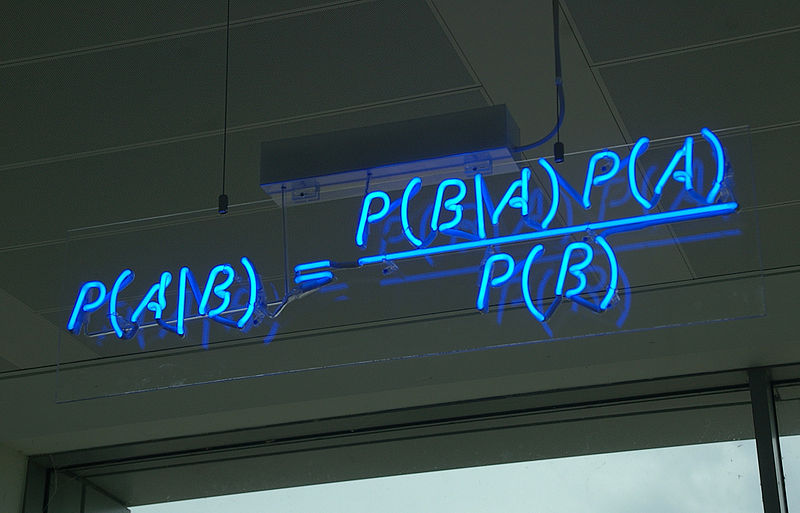
\includegraphics[width=11.11in]{images/bayes_neon}

\}

\textbackslash caption\{Bayes' theorem spelt out in blue neon. Source: \href{https://en.wikipedia.org/wiki/Bayes\%27_theorem}{Wikipedia}\}\label{fig:bayestheorem}
\textbackslash end\{figure\}

I don't know about you, but I need to think twice for not messing the letters around. I find it easier to remember Bayes' theorem written like this\footnote{When teaching Bayes' theorem, I am very much inspired by Tristan Mahr's slides from his introduction to Bayesian regression \url{https://www.tjmahr.com/bayes-intro-lecture-slides-2017/}}:

\[ \Pr(\text{hypothesis} \mid \text{data}) = \frac{ \Pr(\text{data} \mid \text{hypothesis}) \; \Pr(\text{hypothesis})}{\Pr(\text{data})} \]
\begin{rmdnote}
The \emph{hypothesis} is a working assumption about which you want to learn using \emph{data}. In capture--recapture analyses, the hypothesis might be a parameter like detection probability, or regression parameters in a relationship between survival probability and a covariate. Bayes' theorem tells us how to obtain the probability of a hypothesis given the data we have.
\end{rmdnote}

This is great because think about it, this is exactly what the scientific method is! We'd like to know how plausible some hypothesis is based on some data we collected, and possibly compare several hypotheses among them. In that respect, the Bayesian reasoning matches the scientific reasoning, which probably explains why the Bayesian framework is so natural for doing and understanding statistics.

You might ask then, why is Bayesian statistics not the default in statistics? Clearly, because of futile wars between male statisticians (including Ronald Fisher, Jerzy Neyman and Egon Sharpe Pearson among others), little progress was made for over two centuries. Also, until recently, there were practical problems to implement Bayes' theorem. Recent advances in computational power coupled with the development of new algorithms have led to a great increase in the application of Bayesian methods within the last three decades.

\hypertarget{what-is-the-bayesian-approach}{%
\section{What is the Bayesian approach?}\label{what-is-the-bayesian-approach}}

Typical statistical problems involve estimating a parameter (or several parameters) \(\theta\) with available data. To do so, you might be more used to the frequentist rather than the Bayesian method. The frequentist approach, and in particular maximum likelihood estimation (MLE), assumes that the parameters are fixed, and have unknown values to be estimated. Therefore classical estimates are generally point estimates of the parameters of interest. In contrast, the Bayesian approach assumes that the parameters are not fixed, and have some unknown distribution\footnote{A probability distribution is a mathematical expression that gives the probability for a random variable to take particular values. A probability distribution may be either discrete (e.g., the Bernoulli, Binomial or Poisson distribution) or continuous (e.g., the Gaussian distribution also known as the normal distribution)}.

The Bayesian approach is based upon the idea that you, as an experimenter, begin with some prior beliefs about the system. Then you collect data and update your prior beliefs on the basis of observations. These observations might arise from field work, lab work or from expertise of your esteemed colleagues. This updating process is based upon Bayes' theorem. Loosely, let's say \(A = \theta\) and \(B = \text{data}\), then Bayes' theorem gives you a way to estimate parameter \(\theta\) given the data you have:

\[{\color{red}{\Pr(\theta \mid \text{data})}} = \frac{\color{blue}{\Pr(\text{data} \mid \theta)} \times \color{green}{\Pr(\theta)}}{\color{orange}{\Pr(\text{data})}}.\]
Let's spend some time going through each quantity in this formula.

On the left-hand side is the \(\color{red}{\text{posterior distribution}}\). It represents what you know after having seen the data. This is the basis for inference and clearly what you're after, a distribution, possibly multivariate if you have more than one parameter.

On the right-hand side, there is the \(\color{blue}{\text{likelihood}}\). This quantity is the same as in the MLE approach. Yes, the Bayesian and frequentist approaches have the same likelihood at their core, which mostly explains why results often do not differ much. The likelihood captures the information you have in your data, given a model parameterized with \(\theta\).

Then we have the \(\color{green}{\text{prior distribution}}\). This quantity represents what you know before seeing the data. This is the source of much discussion about the Bayesian approach. It may be vague if you don't know anything about \(\theta\). Usually however, you never start from scratch, and you'd like your prior to reflect the information you have\footnote{Shall I include a section on sensitivity analyses in this chapter or later in the book? Cross-reference section in Survival chapter where prior elicitation is covered.}.

Last, we have \(\color{orange}{\Pr(\text{data})}\) which is sometimes called the average likelihood because it is obtained by integrating the likelihood with respect to the prior \(\color{orange}{\Pr(\text{data}) = \int{L(\text{data} \mid \theta)\Pr(\theta) d\theta}}\) so that the posterior is standardized, that is it integrates to one for the posterior to be a distribution. The average likelihood is an integral with dimension the number of parameters \(\theta\) you need to estimate. This quantity is difficult, if not impossible, to calculate in general. This is one of the reasons why the Bayesian method wasn't used until recently, and why we need algorithms to estimate posterior distributions as I illustrate in the next section.

\hypertarget{numerical-approx}{%
\section{Approximating posteriors via numerical integration}\label{numerical-approx}}

Let's take an example to illustrate Bayes' theorem. Say we capture, mark and release \(n = 57\) animals at the beginning of a winter, out of which we recapture \(y = 19\) animals alive\footnote{We used a similar example in \citet{king_bayesian_2009}}. We'd like to estimate winter survival \(\theta\).

\begin{Shaded}
\begin{Highlighting}[]
\NormalTok{y }\OtherTok{\textless{}{-}} \DecValTok{19} \CommentTok{\# nb of success}
\NormalTok{n }\OtherTok{\textless{}{-}} \DecValTok{57} \CommentTok{\# nb of attempts}
\end{Highlighting}
\end{Shaded}

We build our model first. Assuming all animals are independent of each other and have the same survival probability, then \(y\) the number of alive animals at the end of the winter is a binomial distribution\footnote{I follow \citet{mcelreathbook} and use labels on the right to help remember what each line is about.} with \(n\) trials and \(\theta\) the probability of success:

\begin{align*}
y &\sim \text{Binomial}(n, \theta) &\text{[likelihood]}
\end{align*}

This likelihood can be visualised in \texttt{R}:

\begin{Shaded}
\begin{Highlighting}[]
\NormalTok{grid }\OtherTok{\textless{}{-}} \FunctionTok{seq}\NormalTok{(}\DecValTok{0}\NormalTok{, }\DecValTok{1}\NormalTok{, }\FloatTok{0.01}\NormalTok{) }\CommentTok{\# grid of values for survival}
\NormalTok{likelihood }\OtherTok{\textless{}{-}} \FunctionTok{dbinom}\NormalTok{(y, n, grid) }\CommentTok{\# compute binomial likelihood}
\NormalTok{df }\OtherTok{\textless{}{-}} \FunctionTok{data.frame}\NormalTok{(}\AttributeTok{survival =}\NormalTok{ grid, }\AttributeTok{likelihood =}\NormalTok{ likelihood) }
\NormalTok{df }\SpecialCharTok{\%\textgreater{}\%}
  \FunctionTok{ggplot}\NormalTok{() }\SpecialCharTok{+} 
  \FunctionTok{aes}\NormalTok{(}\AttributeTok{x =}\NormalTok{ survival, }\AttributeTok{y =}\NormalTok{ likelihood) }\SpecialCharTok{+} 
  \FunctionTok{geom\_line}\NormalTok{(}\AttributeTok{size =} \FloatTok{1.5}\NormalTok{)}
\end{Highlighting}
\end{Shaded}

\begin{figure}
\centering
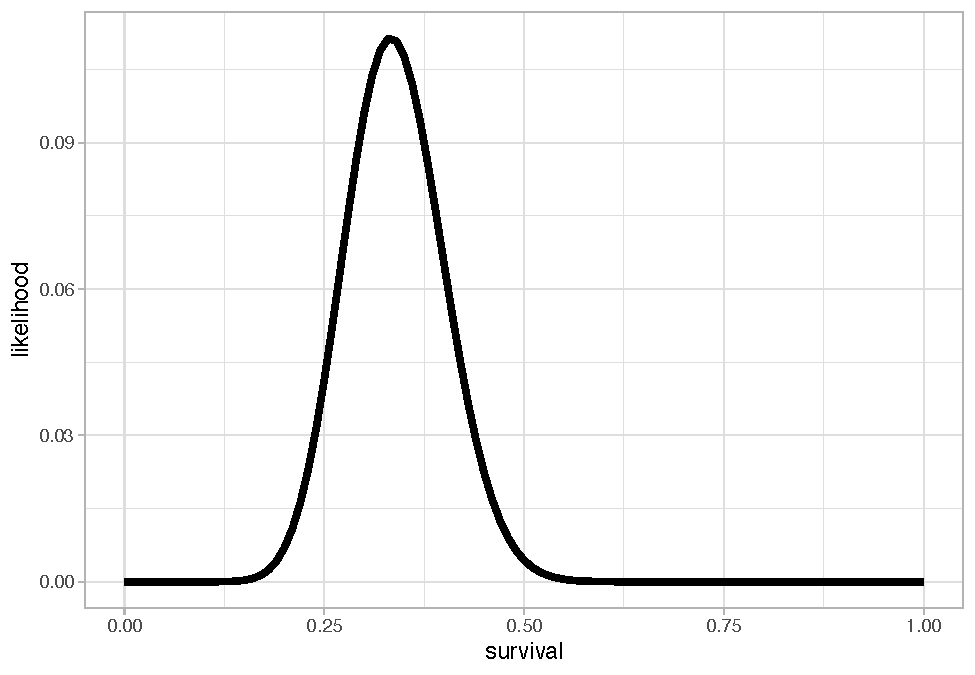
\includegraphics{banana-book_files/figure-latex/binlik-1.pdf}
\caption{\label{fig:binlik}Binomial likelihood with \(n = 57\) released animals and \(y = 19\) survivors after winter. The value of survival (on the x-axis) that corresponds to the maximum of the likelihood function (on the y-axis) is the MLE, or the proportion of success in this example, close to 0.33.}
\end{figure}

Besides the likelihood, priors are another component of the model in the Bayesian approach. For a parameter that is a probability, the one thing we know is that the prior should be a continuous random variable that lies between 0 and 1. To reflect that, we often go for the uniform distribution \(U(0,1)\) to imply \emph{vague} priors. Here vague means that survival has, before we see the data, the same probability of falling between 0.1 and 0.2 and between 0.8 and 0.9, for example.

\begin{align*}
\theta &\sim \text{Uniform}(0, 1) &\text{[prior for }\theta \text{]}
\end{align*}

Now we apply Bayes' theorem. We write a \texttt{R} function that computes the product of the likelihood times the prior, or the numerator in Bayes' theorem: \(\Pr(\text{data} \mid \theta) \times \Pr(\theta)\)

\begin{Shaded}
\begin{Highlighting}[]
\NormalTok{numerator }\OtherTok{\textless{}{-}} \ControlFlowTok{function}\NormalTok{(theta) }\FunctionTok{dbinom}\NormalTok{(y, n, theta) }\SpecialCharTok{*} \FunctionTok{dunif}\NormalTok{(theta, }\DecValTok{0}\NormalTok{, }\DecValTok{1}\NormalTok{)}
\end{Highlighting}
\end{Shaded}

We write another function that calculates the denominator, the average likelihood: \(\Pr(\text{data}) = \int{L(\theta \mid \text{data}) \Pr(\theta) d\theta}\)

\begin{Shaded}
\begin{Highlighting}[]
\NormalTok{denominator }\OtherTok{\textless{}{-}} \FunctionTok{integrate}\NormalTok{(numerator,}\DecValTok{0}\NormalTok{,}\DecValTok{1}\NormalTok{)}\SpecialCharTok{$}\NormalTok{value}
\end{Highlighting}
\end{Shaded}

We use the \texttt{R} function \texttt{integrate} to calculate the integral in the denominator, which implements quadrature techniques to divide in little squares the area underneath the curve delimited by the function to integrate (here the numerator), and count them.

Then we get a numerical approximation of the posterior in Figure \ref{fig:numapprox} by applying Bayes' theorem.

\begin{Shaded}
\begin{Highlighting}[]
\NormalTok{grid }\OtherTok{\textless{}{-}} \FunctionTok{seq}\NormalTok{(}\DecValTok{0}\NormalTok{, }\DecValTok{1}\NormalTok{, }\FloatTok{0.01}\NormalTok{) }\CommentTok{\# grid of values for theta}
\NormalTok{numerical\_posterior }\OtherTok{\textless{}{-}} \FunctionTok{data.frame}\NormalTok{(}\AttributeTok{survival =}\NormalTok{ grid, }
                                  \AttributeTok{posterior =} \FunctionTok{numerator}\NormalTok{(grid)}\SpecialCharTok{/}\NormalTok{denominator) }\CommentTok{\# Bayes\textquotesingle{} theorem}
\NormalTok{numerical\_posterior }\SpecialCharTok{\%\textgreater{}\%}
  \FunctionTok{ggplot}\NormalTok{() }\SpecialCharTok{+}
  \FunctionTok{aes}\NormalTok{(}\AttributeTok{x =}\NormalTok{ survival, }\AttributeTok{y =}\NormalTok{ posterior) }\SpecialCharTok{+} 
  \FunctionTok{geom\_line}\NormalTok{(}\AttributeTok{size =} \FloatTok{1.5}\NormalTok{)}
\end{Highlighting}
\end{Shaded}

\begin{figure}
\centering
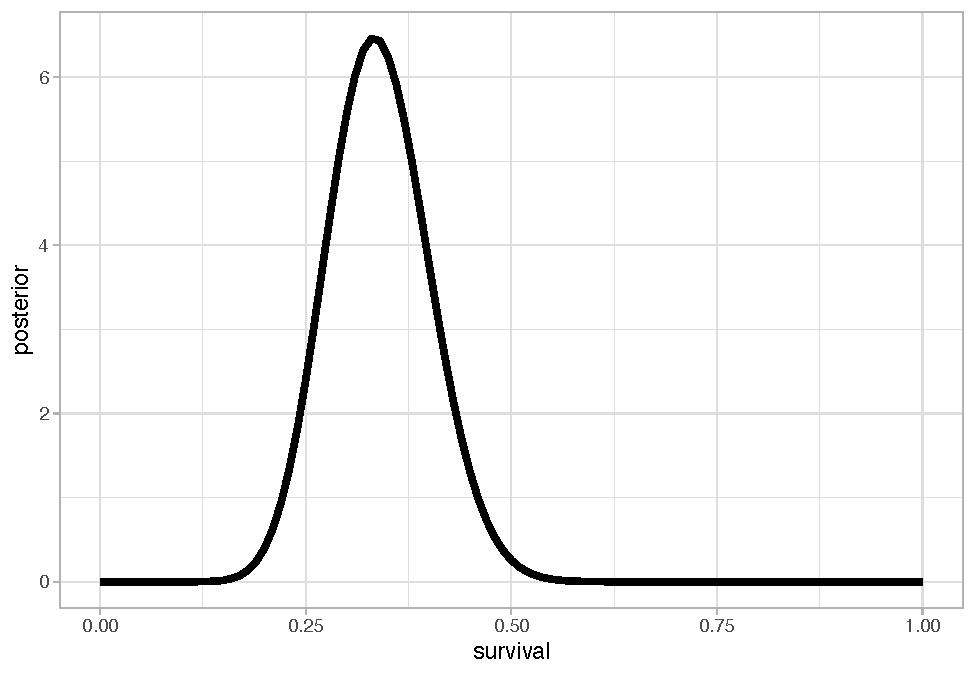
\includegraphics{banana-book_files/figure-latex/numapprox-1.pdf}
\caption{\label{fig:numapprox}Winter survival posterior distribution obtained by numerical integration.}
\end{figure}

How good is our numerical approximation of survival posterior distribution? Ideally, we would want to compare the approximation to the true posterior distribution. Although a closed-form expression for the posterior distribution is in general intractable, when you combine a binomial likelihood together with a beta distribution as a prior, then the posterior distribution is also a beta distribution, which makes it amenable to all sorts of exact calculations\footnote{We say that the beta distribution is the conjugate prior distribution for the binomial distribution.}. The beta distribution is continuous between 0 and 1, and extends the uniform distribution to situations where not all outcomes are equally likely. It has two parameters \(a\) and \(b\) that control its shape (Figure \ref{fig:betadistribution}).



\begin{figure}
\centering
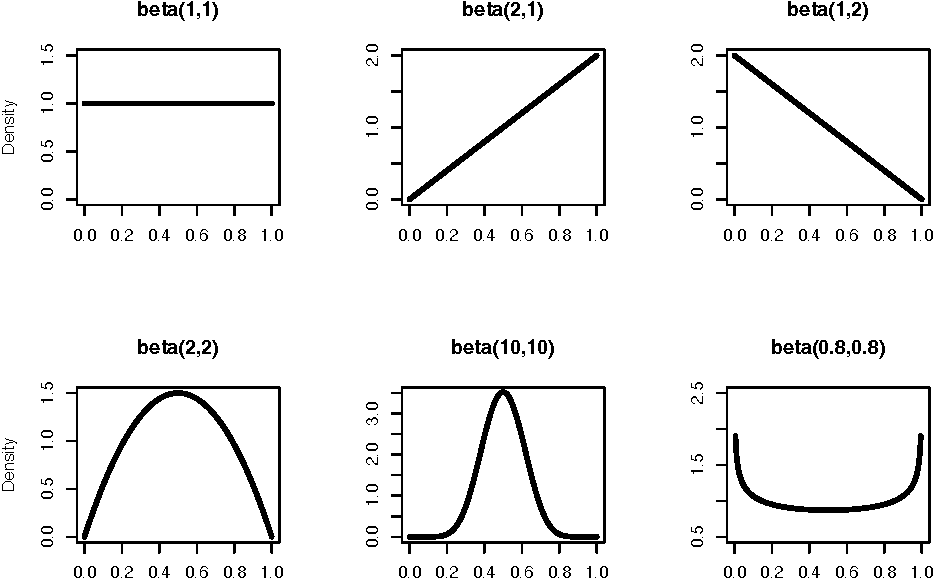
\includegraphics{banana-book_files/figure-latex/betadistribution-1.pdf}
\caption{\label{fig:betadistribution}The distribution beta(\(a\),\(b\)) for different values of \(a\) and \(b\). Note that for \(a = b = 1\), we get the uniform distribution between 0 and 1 in the top left panel. When \(a\) and \(b\) are equal, the distribution is symmetric, and the bigger \(a\) and \(b\), the more peaked the distribution or the smaller the variance.}
\end{figure}

If the likelihood of the data \(y\) is binomial with \(n\) trials and probability of success \(\theta\), and the prior is a beta distribution with parameters \(a\) and \(b\), then the posterior is a beta distribution with parameters \(a + y\) and \(b + n - y\)\footnote{\textbf{provide a sketch of the proof}}. In our example, we have \(n = 57\) trials and \(y = 19\) animals that survived and a uniform prior between 0 and 1 or a beta distribution with parameters \(a = b = 1\), therefore survival has a beta posterior distribution with parameters 20 and 39. In Figure \ref{fig:compar}, we superimpose the exact posterior and the numerical approximation. Clearly, the two distributions are indistinguishable, suggesting that the numerical approximation is more than fine.
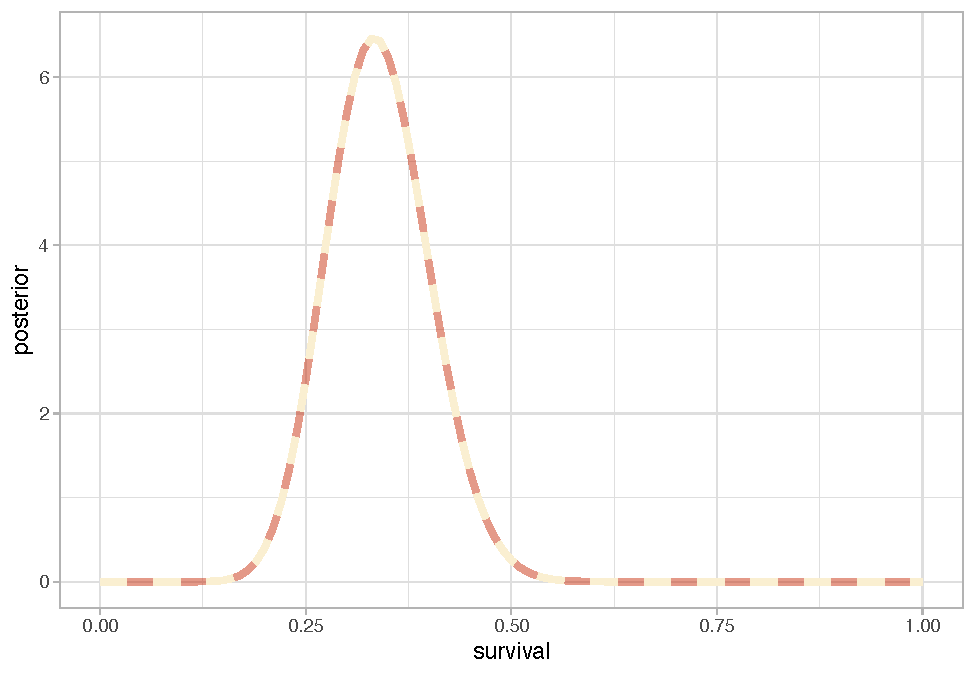
\includegraphics{banana-book_files/figure-latex/compar-1.pdf}

In our example, we have a single parameter to estimate, winter survival. This means dealing with a one-dimensional integral in the denominator which is pretty easy with quadrature techniques and the \texttt{R} function \texttt{integrate()}. Now what if we had multiple parameters? For example, imagine you'd like to fit a capture-recapture model with detection probability \(p\) and regression parameters \(\alpha\) and \(\beta\) for the intercept and slope of a relationship between survival probability and a covariate, then Bayes' theorem gives you the posterior distribution of all three parameters together:

\[ \Pr(\alpha, \beta, p \mid \text{data}) = \frac{ \Pr(\text{data} \mid \alpha, \beta, p) \times \Pr(\alpha, \beta, p)}{\iiint \, \Pr(\text{data} \mid \alpha, \beta, p) \Pr(\alpha, \beta, p) d\alpha d\beta dp} \]
There are two computational challenges with this formula. First, do we really wish to calculate a three-dimensional integral? The answer is no, one-dimensional and two-dimensional integrals are so much further we can go with standard methods. Second, we're more interested in a posterior distribution for each parameter separately than the joint posterior distribution. The so-called marginal distribution of \(p\) for example is obtained by integrating over all the other parameters -- a two-dimensional integral in this example. Now imagine with tens or hundreds of parameters to estimate, these integrals become highly multi-dimensional and simply intractable. In the next section, I introduce powerful simulation methods to circumvent this issue.

\hypertarget{markov-chain-monte-carlo-mcmc}{%
\section{Markov chain Monte Carlo (MCMC)}\label{markov-chain-monte-carlo-mcmc}}

In the early 1990s, statisticians rediscovered work from the 1950's in physics. In a famous paper that would lay the fundations of modern Bayesian statistics (Figure \ref{fig:mcmcpaper}), the authors use simulations to approximate posterior distributions with some precision by drawing large samples. This is a neat trick to avoid explicit calculation of the multi-dimensional integrals we struggle with when using Bayes' theorem.

\begin{figure}

{\centering 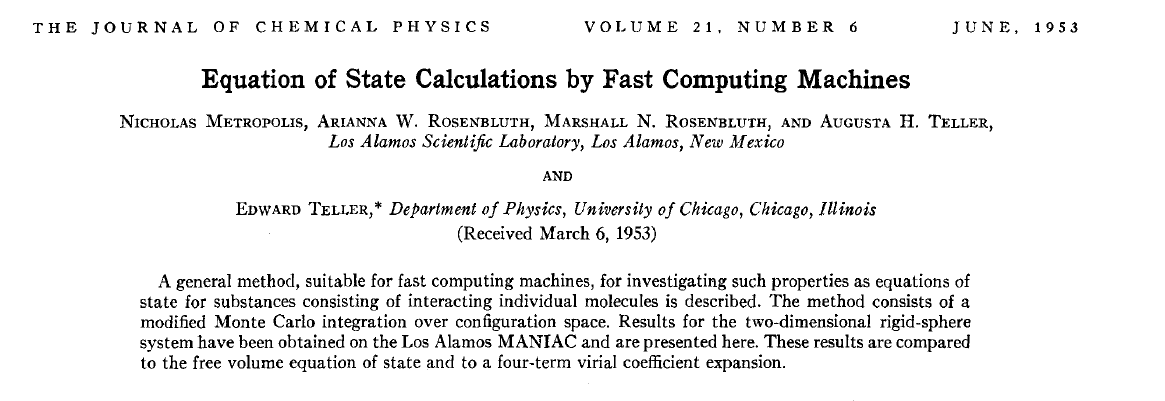
\includegraphics[width=16.18in]{images/metropolis} 

}

\caption{MCMC article cover. Source: [The Journal of Chemical Physics](https://aip.scitation.org/doi/10.1063/1.1699114)}\label{fig:mcmcpaper}
\end{figure}

These simulation algorithms are called Markov chain Monte Carlo (MCMC), and they definitely gave a boost to Bayesian statistics. There are two parts in MCMC, Markov chain and Monte Carlo, let's try and make sense of these terms.

\hypertarget{monte-carlo-integration}{%
\subsection{Monte Carlo integration}\label{monte-carlo-integration}}

What does Monte Carlo stand for? Monte Carlo integration is a simulation technique to calculate integrals of any function \(f\) of random variable \(X\) with distribution \(\Pr(X)\) say \(\int f(X) \Pr(X)dX\). You draw values \(X_1,\ldots,X_k\) from \(\Pr(X)\) the distribution of \(X\), apply function \(f\) to these values, then calculate the mean of these new values \(\displaystyle{\frac{1}{k}}\sum_{i=1}^k{f(X_i)}\) to approximate the integral. How is Monte Carlo integration used in a Bayesian context? The posterior distribution contains all the information we need about the parameter to be estimated. When dealing with many parameters however, you may want to summarise posterior results by calculating numerical summaries. The simplest numerical summary is the mean of the posterior distribution, \(E(\theta) = \int \theta \Pr(\theta|\text{data})\), where \(X\) is \(\theta\) now and \(f\) is the identity function. Posterior mean can be calculated with Monte Carlo integration:

\begin{Shaded}
\begin{Highlighting}[]
\NormalTok{sample\_from\_posterior }\OtherTok{\textless{}{-}} \FunctionTok{rbeta}\NormalTok{(}\DecValTok{1000}\NormalTok{, }\DecValTok{20}\NormalTok{, }\DecValTok{39}\NormalTok{) }\CommentTok{\# draw 1000 values from posterior survival beta(20,39)}
\FunctionTok{mean}\NormalTok{(sample\_from\_posterior) }\CommentTok{\# compute mean with Monte Carlo integration}
\DocumentationTok{\#\# [1] 0.3419}
\end{Highlighting}
\end{Shaded}

You may check that the mean we have just calculated matches closely the expectation of a beta distribution\footnote{If \(X\) is a random variable with distribution \(\text{beta}(a, b)\), then \(E(X) = \displaystyle{\frac{a}{a + b}}\)}:

\begin{Shaded}
\begin{Highlighting}[]
\DecValTok{20}\SpecialCharTok{/}\NormalTok{(}\DecValTok{20}\SpecialCharTok{+}\DecValTok{39}\NormalTok{) }\CommentTok{\# expectation of beta(20,39)}
\DocumentationTok{\#\# [1] 0.339}
\end{Highlighting}
\end{Shaded}

Another useful numerical summary is the credible interval within which our parameter falls with some probability, usually 0.95 hence a 95\(\%\) credible interval. Finding the bounds of a credible interval requires calculating quantiles, which in turn involves integrals and the use of Monte Carlo integration. A 95\(\%\) credible interval for winter survival can be obtained in \texttt{R} with:

\begin{Shaded}
\begin{Highlighting}[]
\FunctionTok{quantile}\NormalTok{(sample\_from\_posterior, }\AttributeTok{probs =} \FunctionTok{c}\NormalTok{(}\FloatTok{2.5}\SpecialCharTok{/}\DecValTok{100}\NormalTok{, }\FloatTok{97.5}\SpecialCharTok{/}\DecValTok{100}\NormalTok{))}
\DocumentationTok{\#\#   2.5\%  97.5\% }
\DocumentationTok{\#\# 0.2256 0.4684}
\end{Highlighting}
\end{Shaded}

\hypertarget{markovmodelmcmc}{%
\subsection{Markov chains}\label{markovmodelmcmc}}

What is a Markov chain? A Markov chain is a random sequence of numbers, in which each number depends only on the previous number. An example is the weather in my home town in Southern France, Montpellier, in which a sunny day is most likely to be followed by another sunny day, say with probability 0.8, and a rainy day is rarely followed by another rainy day, say with probability 0.1. The dynamic of this Markov chain is captured by the transition matrix \(\mathbf{\Gamma}\):
\[
\begin{matrix}
& \\
\mathbf{\Gamma} = 
    \left ( \vphantom{ \begin{matrix} 12 \\ 12 \end{matrix} } \right .
\end{matrix}
\hspace{-1.2em}
\begin{matrix}
    \text{sunny tomorrow} & \text{rainy tomorrow} \\ 
0.8 & 0.2 \\ 
0.9 & 0.1 \\ 
\end{matrix}
\hspace{-0.2em}
\begin{matrix}
& \\
\left . \vphantom{ \begin{matrix} 12 \\ 12 \\ 12 \end{matrix} } \right )
    \begin{matrix}
    \text{sunny today} \\ \text{rainy today}
    \end{matrix}
\end{matrix}
\]
In rows the weather today, and in columns the weather tomorrow. The cells give the probability of a sunny or rainy day tomorrow, given the day is sunny or rainy today. Under certain conditions\footnote{The Markov chain is irreducible and aperiodic.}, a Markov chain will converge to a unique stationary distribution. In our weather example, let's run the Markov chain for 20 steps:

\begin{Shaded}
\begin{Highlighting}[]
\NormalTok{weather }\OtherTok{\textless{}{-}} \FunctionTok{matrix}\NormalTok{(}\FunctionTok{c}\NormalTok{(}\FloatTok{0.8}\NormalTok{, }\FloatTok{0.2}\NormalTok{, }\FloatTok{0.9}\NormalTok{, }\FloatTok{0.1}\NormalTok{), }\AttributeTok{nrow =} \DecValTok{2}\NormalTok{, }\AttributeTok{byrow =}\NormalTok{ T) }\CommentTok{\# transition matrix}
\NormalTok{steps }\OtherTok{\textless{}{-}} \DecValTok{20}
\ControlFlowTok{for}\NormalTok{ (i }\ControlFlowTok{in} \DecValTok{1}\SpecialCharTok{:}\NormalTok{steps)\{}
\NormalTok{  weather }\OtherTok{\textless{}{-}}\NormalTok{ weather }\SpecialCharTok{\%*\%}\NormalTok{ weather }\CommentTok{\# matrix multiplication}
\NormalTok{\}}
\FunctionTok{round}\NormalTok{(weather, }\DecValTok{2}\NormalTok{) }\CommentTok{\# matrix product after 20 steps}
\DocumentationTok{\#\#      [,1] [,2]}
\DocumentationTok{\#\# [1,] 0.82 0.18}
\DocumentationTok{\#\# [2,] 0.82 0.18}
\end{Highlighting}
\end{Shaded}

Each row of the transition matrix converges to the same distribution \((0.82, 0.18)\) as the number of steps increases. Convergence happens no matter which state you start in, and you always have probability 0.82 of the day being sunny and 0.18 of the day being rainy.

Back to MCMC, the core idea is that you can build a Markov chain with a given stationary distribution set to be the desired posterior distribution.

\begin{rmdnote}
Putting Monte Carlo and Markov chains together, MCMC allows us to generate a sample of values (Markov chain) whose distribution converges to the posterior distribution, and we can use this sample of values to calculate any posterior summaries (Monte Carlo), such as posterior means and credible intervals.
\end{rmdnote}

\hypertarget{metropolis-algorithm}{%
\subsection{Metropolis algorithm}\label{metropolis-algorithm}}

There are several ways of constructing Markov chains for Bayesian inference\footnote{You might have heard about the Metropolis-Hastings or the Gibbs sampler. Have a look to \url{https://github.com/chi-feng/mcmc-demo} for an interactive gallery of MCMC algorithms.}. Here I illustrate the Metropolis algorithm and how to implement it in practice\footnote{This presentation is largely inspired by \citet{alberthu2019}}.

Let's go back to our example on animal survival estimation. We illustrate sampling from survival posterior distribution. We write functions for likelihood, prior and posterior.

\begin{Shaded}
\begin{Highlighting}[]
\CommentTok{\# 19 animals recaptured alive out of 57 captured, marked and released}
\NormalTok{survived }\OtherTok{\textless{}{-}} \DecValTok{19}
\NormalTok{released }\OtherTok{\textless{}{-}} \DecValTok{57}

\CommentTok{\# binomial log{-}likelihood function}
\NormalTok{loglikelihood }\OtherTok{\textless{}{-}} \ControlFlowTok{function}\NormalTok{(x, p)\{}
  \FunctionTok{dbinom}\NormalTok{(}\AttributeTok{x =}\NormalTok{ x, }\AttributeTok{size =}\NormalTok{ released, }\AttributeTok{prob =}\NormalTok{ p, }\AttributeTok{log =} \ConstantTok{TRUE}\NormalTok{)}
\NormalTok{\}}

\CommentTok{\# uniform prior density}
\NormalTok{logprior }\OtherTok{\textless{}{-}} \ControlFlowTok{function}\NormalTok{(p)\{}
  \FunctionTok{dunif}\NormalTok{(}\AttributeTok{x =}\NormalTok{ p, }\AttributeTok{min =} \DecValTok{0}\NormalTok{, }\AttributeTok{max =} \DecValTok{1}\NormalTok{, }\AttributeTok{log =} \ConstantTok{TRUE}\NormalTok{)}
\NormalTok{\}}

\CommentTok{\# posterior density function (log scale)}
\NormalTok{posterior }\OtherTok{\textless{}{-}} \ControlFlowTok{function}\NormalTok{(x, p)\{}
  \FunctionTok{loglikelihood}\NormalTok{(x, p) }\SpecialCharTok{+} \FunctionTok{logprior}\NormalTok{(p) }\CommentTok{\# {-} log(Pr(data))}
\NormalTok{\}}
\end{Highlighting}
\end{Shaded}

The Metropolis algorithm works as follows:

\begin{enumerate}
\def\labelenumi{\arabic{enumi}.}
\item
  We pick a value of the parameter to be estimated. This is where we start our Markov chain -- this is a \emph{starting} value.
\item
  To decide where to go next, we propose to move away from the current value of the parameter -- this is a \emph{candidate} value. To do so, we add to the current value some random value from e.g.~a normal distribution with some variance -- this is a \emph{proposal} distribution. The Metropolis algorithm is a particular case of the Metropolis-Hastings algorithm with symmetric proposals.
\item
  We compute the ratio of the probabilities at the candidate and current locations \(R=\displaystyle{\frac{{\Pr(\text{candidate}|\text{data})}}{{\Pr(\text{current}|\text{data})}}}\). This is where the magic of MCMC happens, in that \(\Pr(\text{data})\), the denominator in the Bayes' theorem, appears in both the numerator and the denominator in \(R\) therefore cancels out and does not need to be calculated.
\end{enumerate}

\begin{enumerate}
\def\labelenumi{\arabic{enumi}.}
\setcounter{enumi}{3}
\item
  If the posterior at the candidate location \(\Pr(\text{candidate}|\text{data})\) is higher than at the current location \(\Pr(\text{current}|\text{data})\), in other words when the candidate value is more plausible than the current value, we definitely accept the candidate value. If not, then we accept the candidate value with probability \(R\) and reject with probability \(1-R\). For example, if the candidate value is ten times less plausible than the current value, then we accept with probability 0.1 and reject with probability 0.9. How does it work in practice? We use a continuous spinner that lands somewhere between 0 and 1 -- call the random spin \(X\). If \(X\) is smaller than \(R\), we move to the candidate location, otherwise we remain at the current location. We do not want to accept or reject too often. In practice, the Metropolis algorithm should have an acceptance probability between 0.2 and 0.4, which can be achieved by \emph{tuning} the variance of the normal proposal distribution.
\item
  We repeat 2-4 a number of times -- or \emph{steps}.
\end{enumerate}

Enough of the theory, let's implement the Metropolis algorithm in \texttt{R}. Let's start by setting the scene.

\begin{Shaded}
\begin{Highlighting}[]
\NormalTok{steps }\OtherTok{\textless{}{-}} \DecValTok{100} \CommentTok{\# number of steps}
\NormalTok{theta.post }\OtherTok{\textless{}{-}} \FunctionTok{rep}\NormalTok{(}\ConstantTok{NA}\NormalTok{, steps) }\CommentTok{\# vector to store samples}
\NormalTok{accept }\OtherTok{\textless{}{-}} \FunctionTok{rep}\NormalTok{(}\ConstantTok{NA}\NormalTok{, steps) }\CommentTok{\# keep track of accept/reject}
\FunctionTok{set.seed}\NormalTok{(}\DecValTok{1234}\NormalTok{) }\CommentTok{\# for reproducibility}
\end{Highlighting}
\end{Shaded}

Now follow the 5 steps we've just described. First, we pick a starting value, and store it (step 1).

\begin{Shaded}
\begin{Highlighting}[]
\NormalTok{inits }\OtherTok{\textless{}{-}} \FloatTok{0.5}
\NormalTok{theta.post[}\DecValTok{1}\NormalTok{] }\OtherTok{\textless{}{-}}\NormalTok{ inits}
\NormalTok{accept[}\DecValTok{1}\NormalTok{] }\OtherTok{\textless{}{-}} \DecValTok{1}
\end{Highlighting}
\end{Shaded}

Then, we need a function to propose a candidate value. We add a value taken from a normal distribution with mean zero and standard deviation we call \emph{away}. We work on the logit scale to make sure the candidate value for survival lies between 0 and 1.

\begin{Shaded}
\begin{Highlighting}[]
\NormalTok{move }\OtherTok{\textless{}{-}} \ControlFlowTok{function}\NormalTok{(x, }\AttributeTok{away =} \DecValTok{1}\NormalTok{)\{ }\CommentTok{\# by default, standard deviation of the proposal distribution is 1}
\NormalTok{  logitx }\OtherTok{\textless{}{-}} \FunctionTok{log}\NormalTok{(x }\SpecialCharTok{/}\NormalTok{ (}\DecValTok{1} \SpecialCharTok{{-}}\NormalTok{ x)) }\CommentTok{\# apply logit transform ({-}infinity,+infinity)}
\NormalTok{  logit\_candidate }\OtherTok{\textless{}{-}}\NormalTok{ logitx }\SpecialCharTok{+} \FunctionTok{rnorm}\NormalTok{(}\DecValTok{1}\NormalTok{, }\DecValTok{0}\NormalTok{, away) }\CommentTok{\# add a value taken from N(0,sd=away) to current value}
\NormalTok{  candidate }\OtherTok{\textless{}{-}} \FunctionTok{plogis}\NormalTok{(logit\_candidate) }\CommentTok{\# back{-}transform (0,1)}
  \FunctionTok{return}\NormalTok{(candidate)}
\NormalTok{\}}
\end{Highlighting}
\end{Shaded}

Now we're ready for steps 2, 3 and 4. We write a loop to take care of step 5. We start at initial value 0.5 and run the algorithm for 100 steps or iterations.

\begin{Shaded}
\begin{Highlighting}[]
\ControlFlowTok{for}\NormalTok{ (t }\ControlFlowTok{in} \DecValTok{2}\SpecialCharTok{:}\NormalTok{steps)\{ }\CommentTok{\# repeat steps 2{-}4 (step 5)}
  
  \CommentTok{\# propose candidate value for survival (step 2)}
\NormalTok{  theta\_star }\OtherTok{\textless{}{-}} \FunctionTok{move}\NormalTok{(theta.post[t}\DecValTok{{-}1}\NormalTok{])}
  
  \CommentTok{\# calculate ratio R (step 3)}
\NormalTok{  pstar }\OtherTok{\textless{}{-}} \FunctionTok{posterior}\NormalTok{(survived, }\AttributeTok{p =}\NormalTok{ theta\_star)  }
\NormalTok{  pprev }\OtherTok{\textless{}{-}} \FunctionTok{posterior}\NormalTok{(survived, }\AttributeTok{p =}\NormalTok{ theta.post[t}\DecValTok{{-}1}\NormalTok{])}
\NormalTok{  logR }\OtherTok{\textless{}{-}}\NormalTok{ pstar }\SpecialCharTok{{-}}\NormalTok{ pprev }\CommentTok{\# likelihood and prior are on the log scale}
\NormalTok{  R }\OtherTok{\textless{}{-}} \FunctionTok{exp}\NormalTok{(logR)}
  
  \CommentTok{\# accept candidate value or keep current value (step 4)}
\NormalTok{  X }\OtherTok{\textless{}{-}} \FunctionTok{runif}\NormalTok{(}\DecValTok{1}\NormalTok{, }\DecValTok{0}\NormalTok{, }\DecValTok{1}\NormalTok{) }\CommentTok{\# spin continuous spinner}
  \ControlFlowTok{if}\NormalTok{ (X }\SpecialCharTok{\textless{}}\NormalTok{ R)\{}
\NormalTok{    theta.post[t] }\OtherTok{\textless{}{-}}\NormalTok{ theta\_star }\CommentTok{\# accept candidate value}
\NormalTok{    accept[t] }\OtherTok{\textless{}{-}} \DecValTok{1} \CommentTok{\# accept}
\NormalTok{  \}}
  \ControlFlowTok{else}\NormalTok{\{}
\NormalTok{    theta.post[t] }\OtherTok{\textless{}{-}}\NormalTok{ theta.post[t}\DecValTok{{-}1}\NormalTok{] }\CommentTok{\# keep current value}
\NormalTok{    accept[t] }\OtherTok{\textless{}{-}} \DecValTok{0} \CommentTok{\# reject}
\NormalTok{  \}}
\NormalTok{\}}
\end{Highlighting}
\end{Shaded}

We get the following values.

\begin{Shaded}
\begin{Highlighting}[]
\FunctionTok{head}\NormalTok{(theta.post) }\CommentTok{\# first values}
\DocumentationTok{\#\# [1] 0.5000 0.2302 0.2906 0.2906 0.2980 0.2980}
\FunctionTok{tail}\NormalTok{(theta.post) }\CommentTok{\# last values}
\DocumentationTok{\#\# [1] 0.2622 0.2622 0.2622 0.3727 0.3232 0.3862}
\end{Highlighting}
\end{Shaded}

Visually, you may look at the chain in Figure \ref{fig:chain} called a trace plot.

\begin{figure}

{\centering 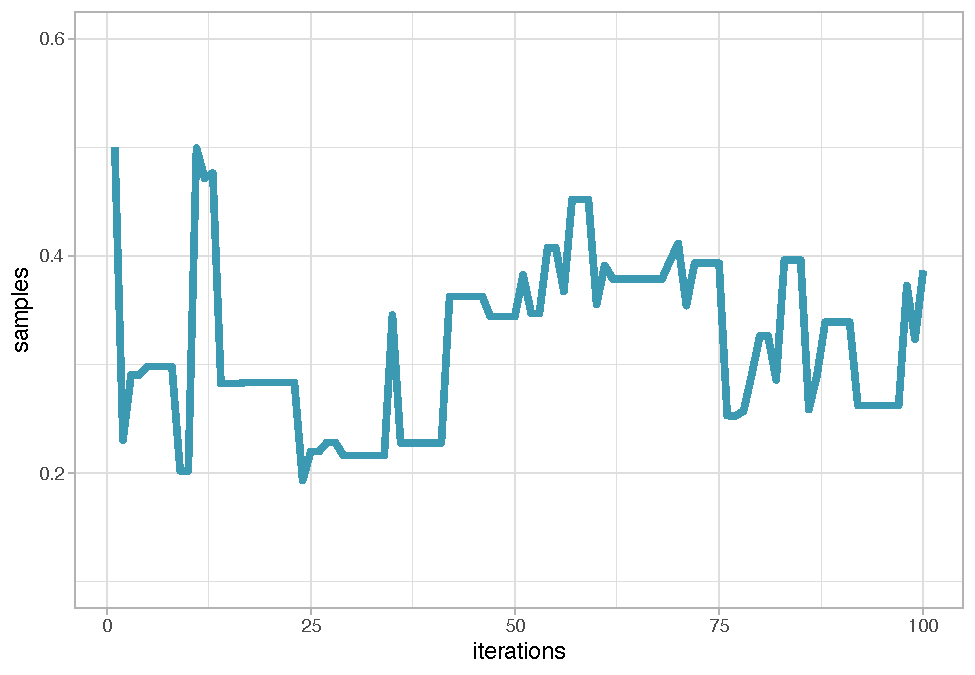
\includegraphics{banana-book_files/figure-latex/chain-1} 

}

\caption{Visualisation of a Markov chain starting at value 0.5, with steps or iterations on the x-axis, and samples on the y-axis. This graphical representation is called a trace plot.}\label{fig:chain}
\end{figure}

The acceptance probability is the average number of times we accepted a candidated value, which is 0.44 and almost satisfying.

Can we run another chain and start at initial value 0.2 this time? Yes, just go through the same algorithm again, and visualise the results in Figure \ref{fig:twochains}.

\begin{figure}

{\centering 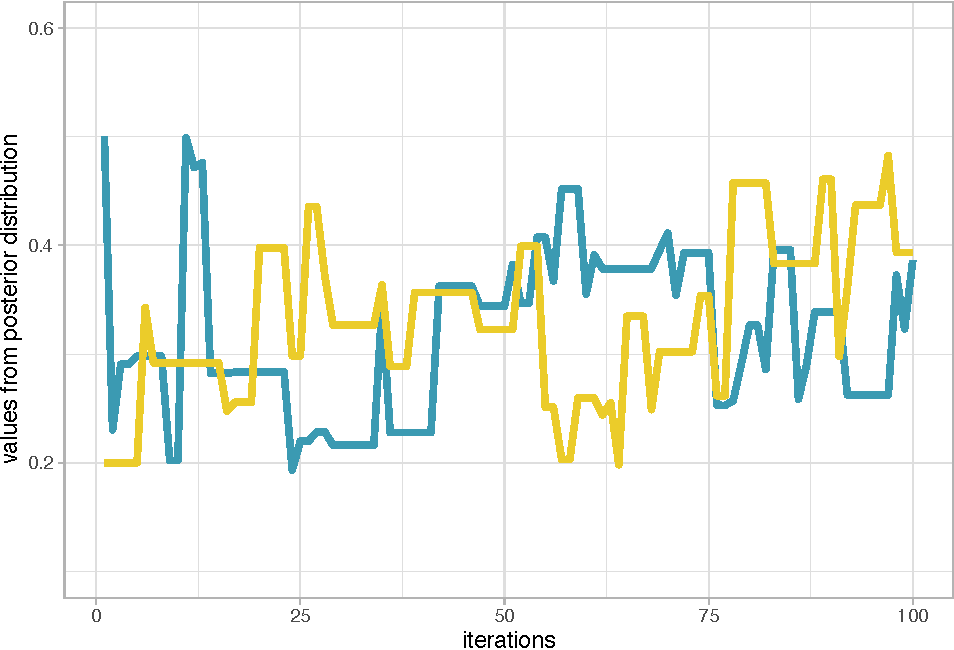
\includegraphics{banana-book_files/figure-latex/twochains-1} 

}

\caption{Trace plot of survival for two chains starting at 0.2 (yellow) and 0.5 (blue) run for 100 steps.}\label{fig:twochains}
\end{figure}

Notice that we do not get the exact same results because the algorithm is stochastic. The question is to know whether we have reached the stationary distribution. Let's increase the number of steps and run a chain with 5000 iterations as in Figure \ref{fig:longchain}.

\begin{figure}

{\centering 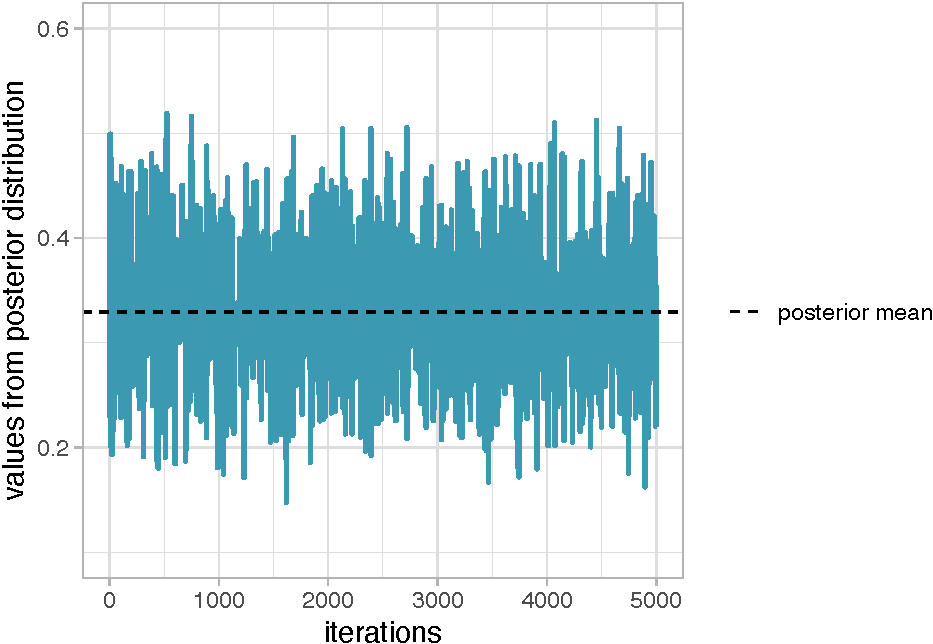
\includegraphics{banana-book_files/figure-latex/longchain-1} 

}

\caption{Trace plot of survival for a chain starting at 0.5 and 1000 steps.}\label{fig:longchain}
\end{figure}

This is what we're after, a trace plot that looks like a beautiful lawn, see Section \ref{convergence-diag}. I find it informative to look at the animated version of Figure \ref{fig:longchain}, it helps understanding the stochastic behavior of the algorithm, and also to realise how the chains converge to their stationary distribution, see Figure \ref{fig:animlongchain}.

\begin{figure}

{\centering \includegraphics[width=1\linewidth]{images/traceplotMCMC} 

}

\caption{Animated trace plot of survival with three chains starting at 0.2, 0.5 and 0.7 run for 1000 steps.}\label{fig:animlongchain}
\end{figure}

Once the stationary distribution is reached, you may regard the realisations of the Markov chain as a sample from the posterior distribution, and obtain numerical summaries. In the next section, we consider several important implementation issues.

\hypertarget{convergence-diag}{%
\section{Assessing convergence}\label{convergence-diag}}

\begin{rmdnote}
When implementing MCMC, we need to determine how long it takes for our Markov chain to converge to the target distribution, and the number of iterations we need after achieving convergence to get reasonable Monte Carlo estimates of numerical summaries (posterior means and credible intervals).
\end{rmdnote}

\hypertarget{burn-in}{%
\subsection{Burn-in}\label{burn-in}}

In practice, we discard observations from the start of the Markov chain and just use observations from the chain once it has converged. The initial observations that we discard are usually referred to as the \emph{burn-in}.

The simplest method to determine the length of the burn-in period is to look at trace plots. Going back to our example, we see from the trace plot in Figure \ref{fig:burnin} that we need at least 100 iterations to achieve convergence toward an average survival around 0.3. It is always better to be conservative when specifying the length of the burn-in period, and in this example, we would use 250 or even 500 iterations as a burn-in. The length of the burn-in period can be determined by performing preliminary MCMC short runs.

\begin{figure}
\centering
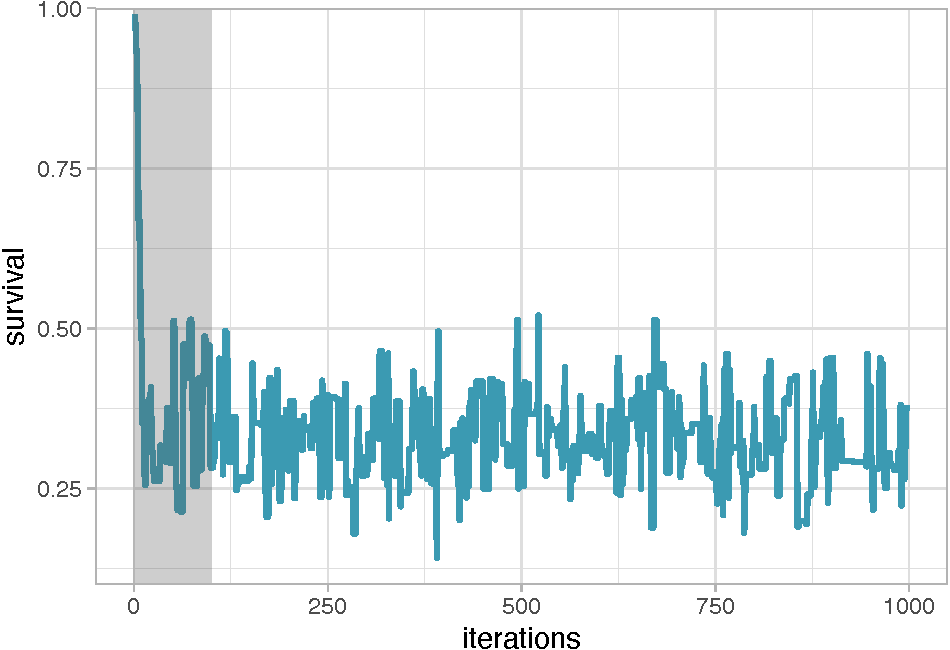
\includegraphics{banana-book_files/figure-latex/burnin-1.pdf}
\caption{\label{fig:burnin}Determining the length of the burn-in period. The chain starts at value 0.99 and rapidly stabilises, with values bouncing back and forth around 0.3 from the 100th iteration onwards. You may choose the shaded area as the burn-in, and discard the corresponding values.}
\end{figure}

Inspecting the trace plot for a single run of the Markov chain is useful. However, we usually run the Markov chain several times, starting from different over-dispersed points, to check that all runs achieve the same stationary distribution. This approach is formalised by using the Brooks-Gelman-Rubin (BGR) statistic \(\hat{R}\) which measures the ratio of the total variability combining multiple chains (between-chain plus within-chain) to the within-chain variability. The BGR statistic asks whether there is a chain effect, and is very much alike the \(F\) test in an analysis of variance. Values below 1.1 indicate likely convergence.

Back to our example, we run two Markov chains with starting values 0.2 and 0.8 using 100 up to 5000 iterations, and calculate the BGR statistic using half the number of iterations as the length of the burn-in. From Figure \ref{fig:bgr}, we get a value of the BGR statistic near 1 by up to 2000 iterations, which suggests that with 2000 iterations as a burn-in, there is no evidence of a lack of convergence.

\begin{figure}
\centering
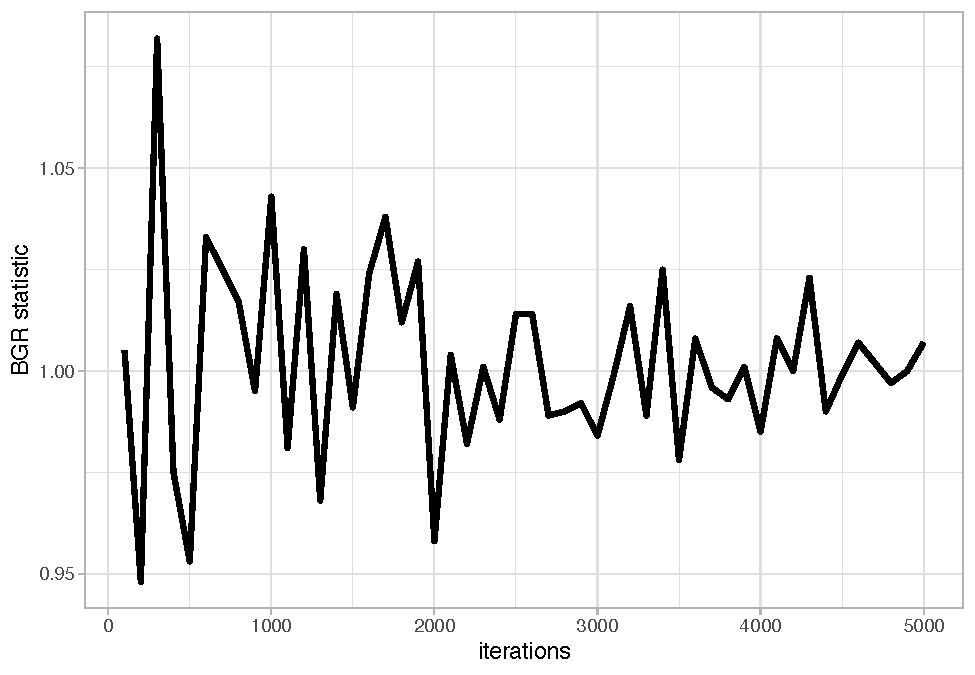
\includegraphics{banana-book_files/figure-latex/bgr-1.pdf}
\caption{\label{fig:bgr}Brooks-Gelman-Rubin statistic as a function of the number of iterations.}
\end{figure}

It is important to bear in mind that a value near 1 for the BGR statistic is only a necessary \emph{but not sufficient} condition for convergence. In other words, this diagnostic cannot tell you for sure that the Markov chain has achieved convergence, only that it has not.\footnote{Cross-reference sections on local minima and parameter redundancy for pathological cases.}

\hypertarget{chain-length}{%
\subsection{Chain length}\label{chain-length}}

How long of a chain is needed to produce reliable parameter estimates? To answer this question, you need to keep in mind that successive steps in a Markov chain are not independent -- this is usually referred to as \emph{autocorrelation}. Ideally, we would like to keep autocorrelation as low as possible. Here again, trace plots are useful to diagnose issues with autocorrelation. Let's get back to our survival example. Figure \ref{fig:tracechainlength} shows trace plots for different values of the standard deviation (parameter \emph{away}) of the (normal) proposal distribution we use to propose a candidate value (Section \ref{metropolis-algorithm}). Small and big moves provide high correlations between successive observations of the Markov chain, whereas a standard deviation of 1 allows efficient exploration of the parameter space. The movement around the parameter space is referred to as \emph{mixing}. Mixing is bad when the chain makes small and big moves, and good otherwise.

\begin{figure}
\centering
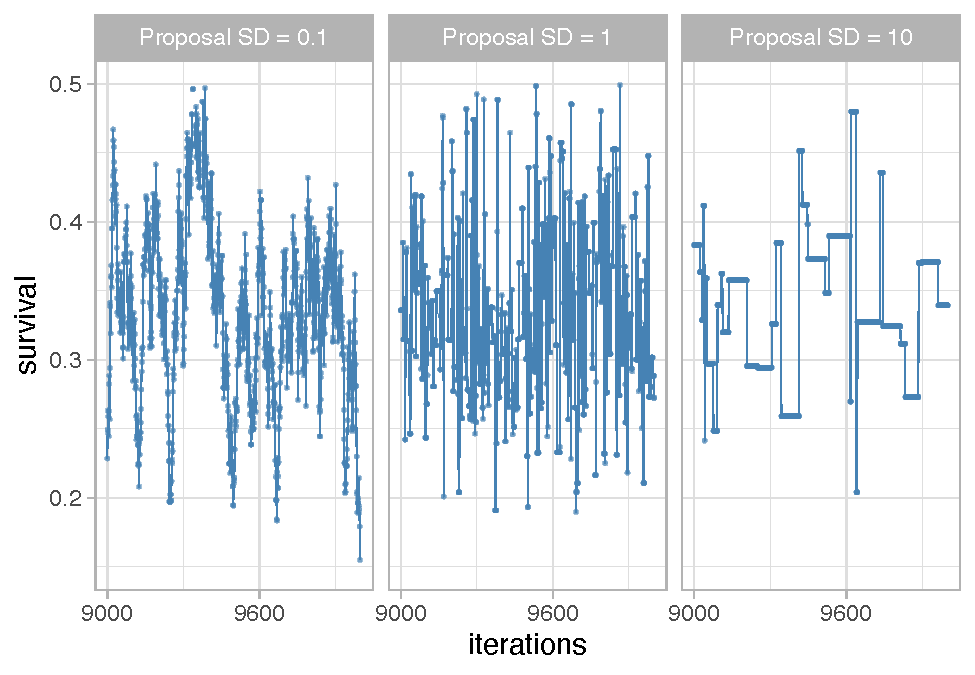
\includegraphics{banana-book_files/figure-latex/tracechainlength-1.pdf}
\caption{\label{fig:tracechainlength}Trace plots for different values of the standard deviation (SD) of the proposal distribution. Left: The chain exhibits small moves and mixing is bad. Right: The chain exhibits big moves and mixing is bad. Middle: The chain exhibits adequate moves and mixing is good. Only the thousand last iterations are shown.}
\end{figure}

In addition to trace plots, autocorrelation function (ACF) plots are a convenient way of displaying the strength of autocorrelation in a given sample values. ACF plots provide the autocorrelation between successively sampled values separated by an increasing number of iterations, or \emph{lag} (Figure \ref{fig:acfchainlength}).

\begin{figure}
\centering
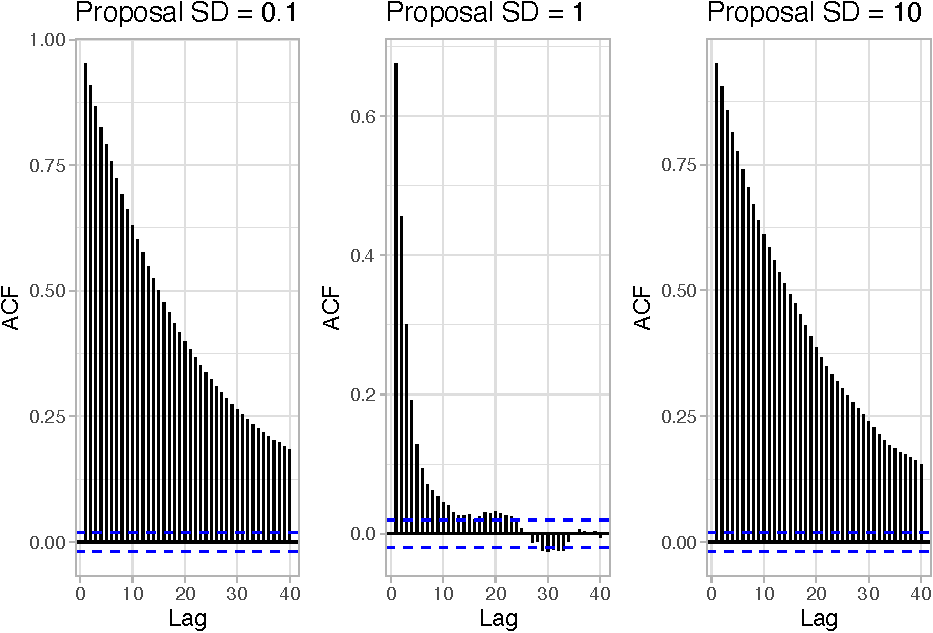
\includegraphics{banana-book_files/figure-latex/acfchainlength-1.pdf}
\caption{\label{fig:acfchainlength}Autocorrelation function plots for different values of the standard deviation (SD) of the proposal distribution. Left and right: Autocorrelation is strong, decreases slowly with increasing lag and mixing is bad. Middle: Autocorrelation is weak, decreases rapidly with increasing lag and mixing is good.}
\end{figure}

Autocorrelation is not necessarily a big issue. Strongly correlated observations just require large sample sizes and therefore longer simulations. But how many iterations exactly? The effective sample size (\texttt{n.eff}) measures chain length while taking into account chain autocorrelation. You should check the \texttt{n.eff} of every parameter of interest, and of any interesting parameter combinations. In general, we need \(\text{n.eff} \geq 1000\) independent steps to get reasonable Monte Carlo estimates of model parameters. In the animal survival example, \texttt{n.eff} can be calculated with the R \texttt{coda::effectiveSize()} function.

\begin{longtable}[]{@{}rr@{}}
\toprule()
Proposal SD & n.eff \\
\midrule()
\endhead
0.1 & 224 \\
1.0 & 1934 \\
10.0 & 230 \\
\bottomrule()
\end{longtable}

As expected, \texttt{n.eff} is less than the number of MCMC iterations because of autocorrelation. Only when the standard deviation of the proposal distribution is 1 and mixing is good (Figures \ref{fig:tracechainlength} and \ref{fig:acfchainlength}) we get a satisfying effective sample size.

\hypertarget{what-if-you-have-issues-of-convergence}{%
\subsection{What if you have issues of convergence?}\label{what-if-you-have-issues-of-convergence}}

When diagnosing MCMC convergence, you will (very) often run into troubles. In this section you will find some helpful tips I hope.

When mixing is bad and effective sample size is small, you may just need to increase burn-in and/or sample more. Using more informative priors might also make Markov chains converge faster by helping your MCMC sampler (e.g.~the Metropolis algorithm) navigating more efficiently the parameter space. In the same spirit, picking better initial values for starting the chain does not harm. For doing that, a strategy consists in using estimates from a simpler model for which your MCMC chains do converge.

If convergence issues persist, often there is a problem with your model\footnote{The quote `When you have computational problems, often there's a problem with your model' is the folk theorem of statistical computing stated by Andrew Gelman in 2008, see \url{https://statmodeling.stat.columbia.edu/2008/05/13/the_folk_theore/}}. A bug in the code? A typo somewhere? A mistake in your maths? As often when coding is involved, the issue can be identified by removing complexities, and start with a simpler model until you find what the problem is.

A general advice is to see your model as a data generating tool in the first place, simulate data from it using some realistic values for the parameters, and try to recover these parameter values by fitting the model to the simulated data. Simulating from a model will help you understanding how it works, what it does not do, and the data you need to get reasonable parameter estimates.

We will see other strategies to improve convergence in the next chapters.\footnote{Cross reference relevant chapters. Option 1. Change your sampler. Option 2. Reparameterize (standardize covariates, plus non-centering: \(\alpha \sim N(0,\sigma)\) becomes \(\alpha = z \sigma\) with \(z \sim N(0,1)\)).}

\hypertarget{summary}{%
\section{Summary}\label{summary}}

\begin{itemize}
\item
  With the Bayes' theorem, you update your beliefs (prior) with new data (likelihood) to get posterior beliefs (posterior): posterior \(\propto\) likelihood \(\times\) prior.
\item
  The idea of Markov chain Monte Carlo (MCMC) is to simulate values from a Markov chain which has a stationary distribution equal to the posterior distribution you're after.
\item
  In practice, you run a Markov chain multiple times starting from over-dispersed initial values.
\item
  You discard iterations in an initial burn-in phase and achieve convergence when all chains reach the same regime.
\item
  From there, you run the chains long enough and proceed with calculating Monte Carlo estimates of numerical summaries (e.g.~posterior means and credible intervals) for parameters.
\end{itemize}

\hypertarget{suggested-reading}{%
\section{Suggested reading}\label{suggested-reading}}

\begin{itemize}
\item
  Gelman, A. and Hill, J. (2006). \href{https://www.cambridge.org/core/books/data-analysis-using-regression-and-multilevelhierarchical-models/32A29531C7FD730C3A68951A17C9D983}{Data Analysis Using Regression and Multilevel/Hierarchical Models (Analytical Methods for Social Research)}. Cambridge: Cambridge University Press.
\item
  Gelman, A. and colleagues (2020). \href{https://arxiv.org/pdf/2011.01808.pdf}{Bayesian workflow}. arXiv preprint.
\item
  McCarthy, M. (2007). \href{https://www.cambridge.org/core/books/bayesian-methods-for-ecology/9225F65B8A25D69B0B6C50B5A9A78201}{Bayesian Methods for Ecology}. Cambridge: Cambridge University Press.
\item
  McElreath, R. (2020). \href{https://xcelab.net/rm/statistical-rethinking/}{Statistical Rethinking: A Bayesian Course with Examples in R and Stan (2nd ed.)}. CRC Press.
\end{itemize}

\hypertarget{intronimble}{%
\chapter{NIMBLE tutorial}\label{intronimble}}

\hypertarget{introduction-2}{%
\section{Introduction}\label{introduction-2}}

In this second chapter, you will get familiar with NIMBLE, an R package that implements up-to-date MCMC algorithms for fitting complex models. NIMBLE spares you from coding the MCMC algorithms by hand, and requires only the specification of a likelihood and priors for model parameters. We will illustrate NIMBLE main features with a simple example, but the ideas hold for other problems.

\hypertarget{what-is-nimble}{%
\section{What is NIMBLE?}\label{what-is-nimble}}

NIMBLE stands for \textbf{N}umerical \textbf{I}nference for statistical \textbf{M}odels using \textbf{B}ayesian and \textbf{L}ikelihood \textbf{E}stimation. Briefly speaking, NIMBLE is an R package that implements for you MCMC algorithms to generate samples from the posterior distribution of model parameters. Freed from the burden of coding your own MCMC algorithms, you only have to specify a likelihood and priors to apply the Bayes theorem. To do so, NIMBLE uses a syntax very similar to the R syntax, which should make your life easier. This so-called BUGS language is also used by other programs like WinBUGS, OpenBUGS, and JAGS.

So why use NIMBLE you may ask? The short answer is that NIMBLE is capable of so much more than just running MCMC algorithms! First, you will work from within R, but in the background NIMBLE will translate your code in C++ for (in general) faster computation. Second, NIMBLE extends the BUGS language for writing new functions and distributions of your own, or borrow those written by others. Third, NIMBLE gives you full control of the MCMC samplers, and you may pick other algorithms than the defaults. Fourth, NIMBLE comes with a library of numerical methods other than MCMC algorithms, including sequential Monte Carlo (for particle filtering) and Monte Carlo Expectation Maximization (for maximum likelihood). Last but not least, the development team is friendly and helpful, and based on users' feedbacks, NIMBLE folks work constantly at improving the package capabilities.

\begin{figure}

{\centering 
\includegraphics[width=0.5\linewidth]{images/nimble-icon} 

}

\caption{Logo of the NIMBLE R package designed by Luke Larson. **Ask Perry for context and meaning.**}\label{fig:nimblelogo}
\end{figure}

\hypertarget{start-nimble}{%
\section{Getting started}\label{start-nimble}}

\begin{rmdnote}
To run NIMBLE, you will need to:\\
1. Build a model consisting of a likelihood and priors.\\
2. Read in some data.\\
3. Specify parameters you want to make inference about.\\
4. Pick initial values for parameters to be estimated (for each chain).\\
5. Provide MCMC details namely the number of chains, the length of the burn-in period and the number of iterations following burn-in.
\end{rmdnote}

First things first, let's not forget to load the \texttt{nimble} package:

\begin{Shaded}
\begin{Highlighting}[]
\FunctionTok{library}\NormalTok{(nimble)}
\end{Highlighting}
\end{Shaded}

Note that before you can install \texttt{nimble} like any other R package, Windows users will need to install \texttt{Rtools}, and Mac users will need to install \texttt{Xcode}. More at \url{https://r-nimble.org/download}.

Now let's go back to our example on animal survival from the previous chapter. First step is to build our model by specifying the binomial likelihood and a uniform prior on survival probability \texttt{theta}. We use the \texttt{nimbleCode()} function and wrap code within curly brackets:

\begin{Shaded}
\begin{Highlighting}[]
\NormalTok{model }\OtherTok{\textless{}{-}} \FunctionTok{nimbleCode}\NormalTok{(\{}
  \CommentTok{\# likelihood}
\NormalTok{  survived }\SpecialCharTok{\textasciitilde{}} \FunctionTok{dbinom}\NormalTok{(theta, released)}
  \CommentTok{\# prior}
\NormalTok{  theta }\SpecialCharTok{\textasciitilde{}} \FunctionTok{dunif}\NormalTok{(}\DecValTok{0}\NormalTok{, }\DecValTok{1}\NormalTok{)}
  \CommentTok{\# derived quantity}
\NormalTok{  lifespan }\OtherTok{\textless{}{-}} \SpecialCharTok{{-}}\DecValTok{1}\SpecialCharTok{/}\FunctionTok{log}\NormalTok{(theta)}
\NormalTok{\})}
\end{Highlighting}
\end{Shaded}

You can check that the \texttt{model} R object contains your code:

\begin{Shaded}
\begin{Highlighting}[]
\NormalTok{model}
\DocumentationTok{\#\# \{}
\DocumentationTok{\#\#     survived \textasciitilde{} dbinom(theta, released)}
\DocumentationTok{\#\#     theta \textasciitilde{} dunif(0, 1)}
\DocumentationTok{\#\#     lifespan \textless{}{-} {-}1/log(theta)}
\DocumentationTok{\#\# \}}
\end{Highlighting}
\end{Shaded}

In the code above, \texttt{survived} and \texttt{released} are known, only \texttt{theta} needs to be estimated. The line \texttt{survived\ \textasciitilde{}\ dbinom(theta,\ released)} states that the number of successes or animals that have survived over winter \texttt{survived} is distributed as (that's the \texttt{\textasciitilde{}}) as a binomial with \texttt{released} trials and probability of success or survival \texttt{theta}. Then the line \texttt{theta\ \textasciitilde{}\ dunif(0,\ 1)} assigns a uniform between 0 and 1 as a prior distribution to the survival probability. This is all you need, a likelihood and priors for model parameters, NIMBLE knows the Bayes theorem. The last line \texttt{lifespan\ \textless{}-\ -\ 1/log(theta)} calculates a quantity derived from \texttt{theta}, which is the expected lifespan assuming constant survival\footnote{Cook LM, Brower LP, Croze HJ (1967) The accuracy of a population estimation from multiple recapture data. J Anim Ecol 36:57--60}.

A few comments:

\begin{itemize}
\item
  The most common distributions are available in NIMBLE. Among others, we will use later in the book \texttt{dbeta}, \texttt{dmultinom} and \texttt{dnorm}. If you cannot find what you need in NIMBLE, you can write your own distribution as illustrated in Section \ref{functions-in-nimble}.
\item
  It does not matter in what order you write each line of code, NIMBLE uses what is called a declarative language for building models. In brief, you write code that tells NIMBLE what you want to achieve, and not how to get there. In contrast, an imperative language requires that you write what you want your program to do step by step.
\item
  You can think of models in NIMBLE as graphs as in Figure \ref{fig:dag-survival}. A graph is made of relations (or edges) that can be of two types. A stochastic relation is signaled by a \texttt{\textasciitilde{}} sign and defines a random variable in the model, such as \texttt{survived} or \texttt{theta}. A deterministic relation is signaled by a \texttt{\textless{}-} sign, like \texttt{lifespan}. Relations define nodes on the left - the children - in terms of other nodes on the right - the parents, and relations are directed edges from parents to children. Such graphs are called directed acyclic graph or DAG.
  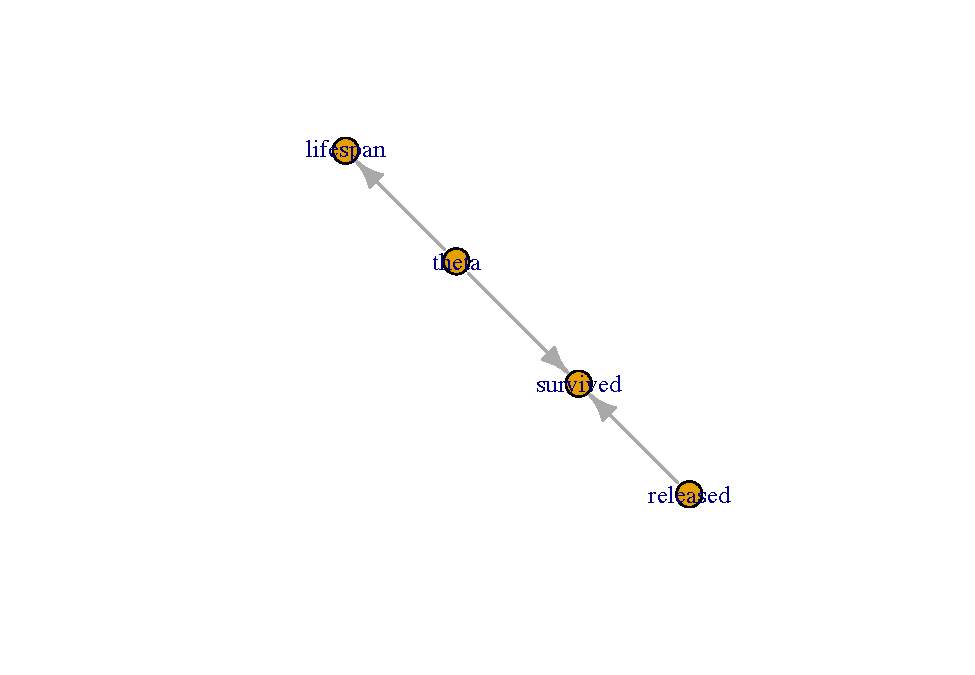
\includegraphics{banana-book_files/figure-latex/dag-survival-1.pdf}
\end{itemize}

Second step in our workflow is to read in some data. We use a list in which each component corresponds to a known quantity in the model:

\begin{Shaded}
\begin{Highlighting}[]
\NormalTok{my.data }\OtherTok{\textless{}{-}} \FunctionTok{list}\NormalTok{(}\AttributeTok{released =} \DecValTok{57}\NormalTok{, }\AttributeTok{survived =} \DecValTok{19}\NormalTok{)}
\end{Highlighting}
\end{Shaded}

You can proceed with data passed this way, but you should know a little more about how NIMBLE sees data. NIMBLE distinguishes data and constants. Constants are values that do not change, e.g.~vectors of known index values or the indices used to define for loops. Data are values that you might want to change, basically anything that only appears on the left of a \texttt{\textasciitilde{}}. Declaring relevant values as constants is better for computational efficiency, but it is easy to forget, and fortunately NIMBLE will by itself distinguish data and constants. I will not use the distinction between data and constants in this chapter, but in the next chapters it will become important.

Third step is to tell NIMBLE which nodes in your model you would like to keep track of, in other words the quantities you'd like to do inference about. In our model we want survival \texttt{theta} and \texttt{lifespan}:

\begin{Shaded}
\begin{Highlighting}[]
\NormalTok{parameters.to.save }\OtherTok{\textless{}{-}} \FunctionTok{c}\NormalTok{(}\StringTok{"theta"}\NormalTok{, }\StringTok{"lifespan"}\NormalTok{)}
\end{Highlighting}
\end{Shaded}

In general you have many quantities in your model, including some of little interest that are not worth monitoring, and having full control on verbosity will prove handy.

Fourth step is to specify initial values for all model parameters. To make sure that the MCMC algorithm explores the posterior distribution, we start different chains with different parameter values. You can specify initial values for each chain in a list and put them in yet another list:

\begin{Shaded}
\begin{Highlighting}[]
\NormalTok{init1 }\OtherTok{\textless{}{-}} \FunctionTok{list}\NormalTok{(}\AttributeTok{theta =} \FloatTok{0.1}\NormalTok{)}
\NormalTok{init2 }\OtherTok{\textless{}{-}} \FunctionTok{list}\NormalTok{(}\AttributeTok{theta =} \FloatTok{0.5}\NormalTok{)}
\NormalTok{init3 }\OtherTok{\textless{}{-}} \FunctionTok{list}\NormalTok{(}\AttributeTok{theta =} \FloatTok{0.9}\NormalTok{)}
\NormalTok{initial.values }\OtherTok{\textless{}{-}} \FunctionTok{list}\NormalTok{(init1, init2, init3)}
\NormalTok{initial.values}
\DocumentationTok{\#\# [[1]]}
\DocumentationTok{\#\# [[1]]$theta}
\DocumentationTok{\#\# [1] 0.1}
\DocumentationTok{\#\# }
\DocumentationTok{\#\# }
\DocumentationTok{\#\# [[2]]}
\DocumentationTok{\#\# [[2]]$theta}
\DocumentationTok{\#\# [1] 0.5}
\DocumentationTok{\#\# }
\DocumentationTok{\#\# }
\DocumentationTok{\#\# [[3]]}
\DocumentationTok{\#\# [[3]]$theta}
\DocumentationTok{\#\# [1] 0.9}
\end{Highlighting}
\end{Shaded}

Alternatively, you can write a simple R function that generates random initial values:

\begin{Shaded}
\begin{Highlighting}[]
\NormalTok{initial.values }\OtherTok{\textless{}{-}} \ControlFlowTok{function}\NormalTok{() }\FunctionTok{list}\NormalTok{(}\AttributeTok{theta =} \FunctionTok{runif}\NormalTok{(}\DecValTok{1}\NormalTok{,}\DecValTok{0}\NormalTok{,}\DecValTok{1}\NormalTok{))}
\FunctionTok{initial.values}\NormalTok{()}
\DocumentationTok{\#\# $theta}
\DocumentationTok{\#\# [1] 0.8356}
\end{Highlighting}
\end{Shaded}

Firth and last step, you need to tell NIMBLE the number of chains to run, say \texttt{n.chain}, how long the burn-in period should be, say \texttt{n.burnin}, and the number of iterations following the burn-in period to be used for posterior inference. In NIMBLE, you specify the total number of iterations, say \texttt{n.iter}, so that the number of posterior samples per chain is \texttt{n.iter\ -\ n.burnin}. NIMBLE also allows discarding samples after burn-in, a procedure known as thinning, which I will not use in this book\footnote{Link, W.A. and Eaton, M.J. (2012), On thinning of chains in MCMC. Methods in Ecology and Evolution, 3: 112-115.}.

\begin{Shaded}
\begin{Highlighting}[]
\NormalTok{n.iter }\OtherTok{\textless{}{-}} \DecValTok{5000}
\NormalTok{n.burnin }\OtherTok{\textless{}{-}} \DecValTok{1000}
\NormalTok{n.chains }\OtherTok{\textless{}{-}} \DecValTok{3}
\end{Highlighting}
\end{Shaded}

We now have all the ingredients to run model, that is to sample in the posterior distribution of model parameters using MCMC simulations. This is accomplished using function \texttt{nimbleMCMC()}:

\begin{Shaded}
\begin{Highlighting}[]
\NormalTok{mcmc.output }\OtherTok{\textless{}{-}} \FunctionTok{nimbleMCMC}\NormalTok{(}\AttributeTok{code =}\NormalTok{ model,}
                          \AttributeTok{data =}\NormalTok{ my.data,}
                          \AttributeTok{inits =}\NormalTok{ initial.values,}
                          \AttributeTok{monitors =}\NormalTok{ parameters.to.save,}
                          \AttributeTok{niter =}\NormalTok{ n.iter,}
                          \AttributeTok{nburnin =}\NormalTok{ n.burnin,}
                          \AttributeTok{nchains =}\NormalTok{ n.chains)}
\DocumentationTok{\#\# |{-}{-}{-}{-}{-}{-}{-}{-}{-}{-}{-}{-}{-}|{-}{-}{-}{-}{-}{-}{-}{-}{-}{-}{-}{-}{-}|{-}{-}{-}{-}{-}{-}{-}{-}{-}{-}{-}{-}{-}|{-}{-}{-}{-}{-}{-}{-}{-}{-}{-}{-}{-}{-}|}
\DocumentationTok{\#\# |{-}{-}{-}{-}{-}{-}{-}{-}{-}{-}{-}{-}{-}{-}{-}{-}{-}{-}{-}{-}{-}{-}{-}{-}{-}{-}{-}{-}{-}{-}{-}{-}{-}{-}{-}{-}{-}{-}{-}{-}{-}{-}{-}{-}{-}{-}{-}{-}{-}{-}{-}{-}{-}{-}{-}|}
\DocumentationTok{\#\# |{-}{-}{-}{-}{-}{-}{-}{-}{-}{-}{-}{-}{-}|{-}{-}{-}{-}{-}{-}{-}{-}{-}{-}{-}{-}{-}|{-}{-}{-}{-}{-}{-}{-}{-}{-}{-}{-}{-}{-}|{-}{-}{-}{-}{-}{-}{-}{-}{-}{-}{-}{-}{-}|}
\DocumentationTok{\#\# |{-}{-}{-}{-}{-}{-}{-}{-}{-}{-}{-}{-}{-}{-}{-}{-}{-}{-}{-}{-}{-}{-}{-}{-}{-}{-}{-}{-}{-}{-}{-}{-}{-}{-}{-}{-}{-}{-}{-}{-}{-}{-}{-}{-}{-}{-}{-}{-}{-}{-}{-}{-}{-}{-}{-}|}
\DocumentationTok{\#\# |{-}{-}{-}{-}{-}{-}{-}{-}{-}{-}{-}{-}{-}|{-}{-}{-}{-}{-}{-}{-}{-}{-}{-}{-}{-}{-}|{-}{-}{-}{-}{-}{-}{-}{-}{-}{-}{-}{-}{-}|{-}{-}{-}{-}{-}{-}{-}{-}{-}{-}{-}{-}{-}|}
\DocumentationTok{\#\# |{-}{-}{-}{-}{-}{-}{-}{-}{-}{-}{-}{-}{-}{-}{-}{-}{-}{-}{-}{-}{-}{-}{-}{-}{-}{-}{-}{-}{-}{-}{-}{-}{-}{-}{-}{-}{-}{-}{-}{-}{-}{-}{-}{-}{-}{-}{-}{-}{-}{-}{-}{-}{-}{-}{-}|}
\end{Highlighting}
\end{Shaded}

NIMBLE goes through several steps that we will explain in Section \ref{under-the-hood}. Function \texttt{nimbleMCMC()} takes other arguments that you might find useful. For example, you can suppress the progress bar if you find it too depressing when running long simulations with \texttt{progressBar\ =\ FALSE}. You can also get a summary of the outputs by specifying \texttt{summary\ =\ TRUE}. Check \texttt{?nimbleMCMC} for more details.

Now let's inspect what we have in \texttt{mcmc.output}:

\begin{Shaded}
\begin{Highlighting}[]
\FunctionTok{str}\NormalTok{(mcmc.output)}
\DocumentationTok{\#\# List of 3}
\DocumentationTok{\#\#  $ chain1: num [1:4000, 1:2] 0.907 0.907 0.907 0.907 0.853 ...}
\DocumentationTok{\#\#   ..{-} attr(*, "dimnames")=List of 2}
\DocumentationTok{\#\#   .. ..$ : NULL}
\DocumentationTok{\#\#   .. ..$ : chr [1:2] "lifespan" "theta"}
\DocumentationTok{\#\#  $ chain2: num [1:4000, 1:2] 0.787 0.894 1.291 1.388 1.388 ...}
\DocumentationTok{\#\#   ..{-} attr(*, "dimnames")=List of 2}
\DocumentationTok{\#\#   .. ..$ : NULL}
\DocumentationTok{\#\#   .. ..$ : chr [1:2] "lifespan" "theta"}
\DocumentationTok{\#\#  $ chain3: num [1:4000, 1:2] 0.745 0.745 0.745 0.886 1.136 ...}
\DocumentationTok{\#\#   ..{-} attr(*, "dimnames")=List of 2}
\DocumentationTok{\#\#   .. ..$ : NULL}
\DocumentationTok{\#\#   .. ..$ : chr [1:2] "lifespan" "theta"}
\end{Highlighting}
\end{Shaded}

The R object \texttt{mcmc.output} is a list with three components, one for each MCMC chain. Let's have a look to \texttt{chain1} for example:

\begin{Shaded}
\begin{Highlighting}[]
\FunctionTok{dim}\NormalTok{(mcmc.output}\SpecialCharTok{$}\NormalTok{chain1)}
\DocumentationTok{\#\# [1] 4000    2}
\FunctionTok{head}\NormalTok{(mcmc.output}\SpecialCharTok{$}\NormalTok{chain1)}
\DocumentationTok{\#\#      lifespan  theta}
\DocumentationTok{\#\# [1,]   0.9069 0.3320}
\DocumentationTok{\#\# [2,]   0.9069 0.3320}
\DocumentationTok{\#\# [3,]   0.9069 0.3320}
\DocumentationTok{\#\# [4,]   0.9069 0.3320}
\DocumentationTok{\#\# [5,]   0.8526 0.3095}
\DocumentationTok{\#\# [6,]   0.7987 0.2859}
\end{Highlighting}
\end{Shaded}

Each component of the list is a matrix. In rows, you have 4000 samples from the posterior distribution of \texttt{theta}, which corresponds to \texttt{n.iter\ -\ n.burnin} iterations. In columns, you have the quantities we monitor, \texttt{theta} and \texttt{lifespan}. From there, you can compute the posterior mean of \texttt{theta}:

\begin{Shaded}
\begin{Highlighting}[]
\FunctionTok{mean}\NormalTok{(mcmc.output}\SpecialCharTok{$}\NormalTok{chain1[,}\StringTok{\textquotesingle{}theta\textquotesingle{}}\NormalTok{])}
\DocumentationTok{\#\# [1] 0.3407}
\end{Highlighting}
\end{Shaded}

You can also obtain the 95\% credible interval for \texttt{theta}:

\begin{Shaded}
\begin{Highlighting}[]
\FunctionTok{quantile}\NormalTok{(mcmc.output}\SpecialCharTok{$}\NormalTok{chain1[,}\StringTok{\textquotesingle{}theta\textquotesingle{}}\NormalTok{], }\AttributeTok{probs =} \FunctionTok{c}\NormalTok{(}\FloatTok{2.5}\NormalTok{, }\FloatTok{97.5}\NormalTok{)}\SpecialCharTok{/}\DecValTok{100}\NormalTok{)}
\DocumentationTok{\#\#   2.5\%  97.5\% }
\DocumentationTok{\#\# 0.2219 0.4620}
\end{Highlighting}
\end{Shaded}

Let's visualise the posterior distribution of \texttt{theta} with a histogram:

\begin{Shaded}
\begin{Highlighting}[]
\NormalTok{mcmc.output }\SpecialCharTok{\%\textgreater{}\%}
  \FunctionTok{as\_tibble}\NormalTok{() }\SpecialCharTok{\%\textgreater{}\%}
  \FunctionTok{ggplot}\NormalTok{() }\SpecialCharTok{+}
  \FunctionTok{geom\_histogram}\NormalTok{(}\FunctionTok{aes}\NormalTok{(}\AttributeTok{x =}\NormalTok{ chain1[,}\StringTok{"theta"}\NormalTok{]), }\AttributeTok{color =} \StringTok{"white"}\NormalTok{) }\SpecialCharTok{+}
  \FunctionTok{labs}\NormalTok{(}\AttributeTok{x =} \StringTok{"survival probability"}\NormalTok{)}
\end{Highlighting}
\end{Shaded}

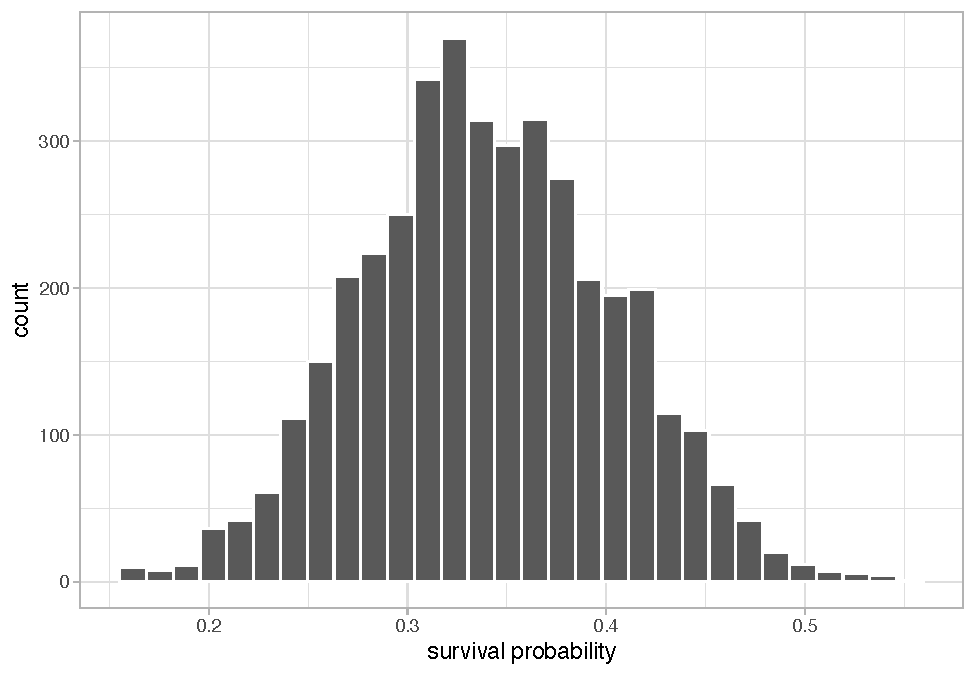
\includegraphics{banana-book_files/figure-latex/unnamed-chunk-43-1.pdf}

There are less painful ways of doing posterior inference. In this book, I will use the R package \texttt{MCMCvis}\footnote{\url{https://github.com/caseyyoungflesh/MCMCvis}} to summarise and visualize MCMC outputs, but there are other perfectly valid options out there like \texttt{ggmcmc}\footnote{Fernández-i-Marín, X. (2016). ggmcmc: Analysis of MCMC Samples and Bayesian Inference. Journal of Statistical Software, 70(9), 1--20} and \texttt{basicMCMCplots}\footnote{\url{https://cran.r-project.org/web/packages/basicMCMCplots/index.html}}. \textbf{Shall I demonstrate these other options?}

Let's load the package \texttt{MCMCvis}:

\begin{Shaded}
\begin{Highlighting}[]
\FunctionTok{library}\NormalTok{(MCMCvis)}
\end{Highlighting}
\end{Shaded}

To get the most common numerical summaries, the function \texttt{MCMCsummary()} does the job:

\begin{Shaded}
\begin{Highlighting}[]
\FunctionTok{MCMCsummary}\NormalTok{(}\AttributeTok{object =}\NormalTok{ mcmc.output, }\AttributeTok{round =} \DecValTok{2}\NormalTok{)}
\DocumentationTok{\#\#          mean   sd 2.5\%  50\% 97.5\% Rhat n.eff}
\DocumentationTok{\#\# lifespan 0.94 0.17 0.66 0.92  1.32    1  2513}
\DocumentationTok{\#\# theta    0.34 0.06 0.22 0.34  0.47    1  2533}
\end{Highlighting}
\end{Shaded}

You can use a caterpillar plot to visualise the posterior distributions of \texttt{theta} with \texttt{MCMCplot()}:

\begin{Shaded}
\begin{Highlighting}[]
\FunctionTok{MCMCplot}\NormalTok{(}\AttributeTok{object =}\NormalTok{ mcmc.output, }
         \AttributeTok{params =} \StringTok{\textquotesingle{}theta\textquotesingle{}}\NormalTok{)}
\end{Highlighting}
\end{Shaded}

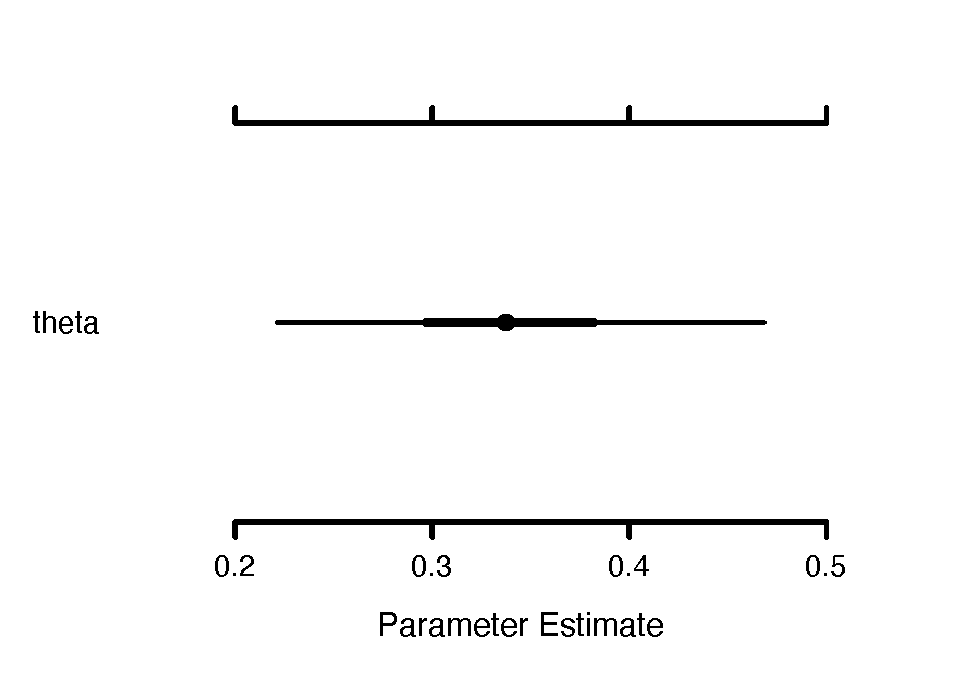
\includegraphics{banana-book_files/figure-latex/unnamed-chunk-46-1.pdf}

The point represents the posterior median, the thick line is the 50\% credible interval and the thin line the 95\% credible interval.

The trace and posterior density of theta can be obtained with \texttt{MCMCtrace()}:

\begin{Shaded}
\begin{Highlighting}[]
\FunctionTok{MCMCtrace}\NormalTok{(}\AttributeTok{object =}\NormalTok{ mcmc.output,}
          \AttributeTok{pdf =} \ConstantTok{FALSE}\NormalTok{, }\CommentTok{\# no export to PDF}
          \AttributeTok{ind =} \ConstantTok{TRUE}\NormalTok{, }\CommentTok{\# separate density lines per chain}
          \AttributeTok{params =} \StringTok{"theta"}\NormalTok{)}
\end{Highlighting}
\end{Shaded}

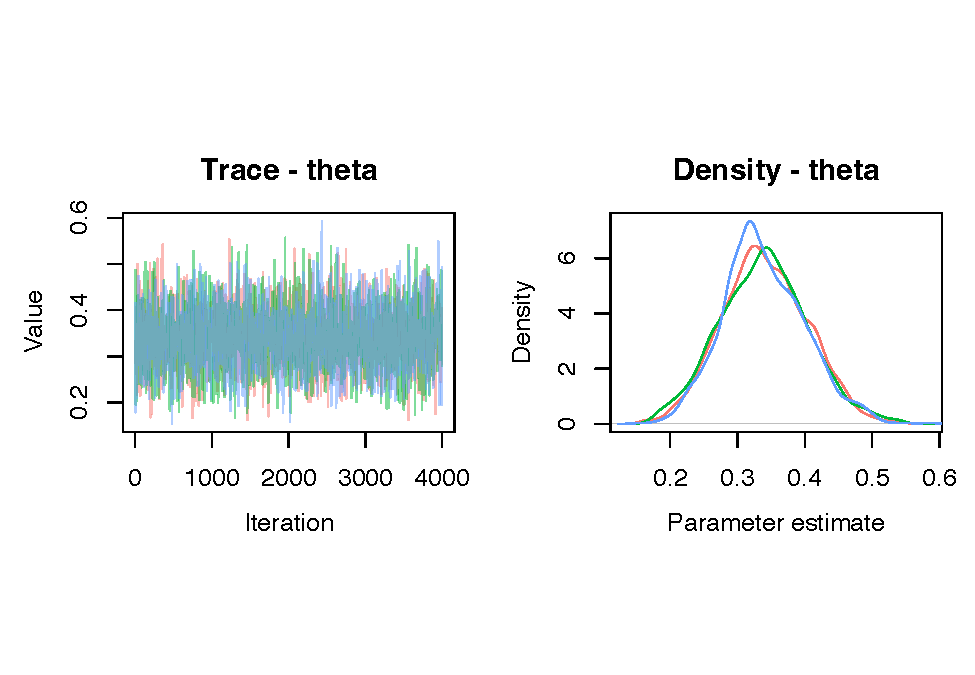
\includegraphics{banana-book_files/figure-latex/unnamed-chunk-47-1.pdf}

You can also add the diagnostics of convergence we discussed in the previous chapter:

\begin{Shaded}
\begin{Highlighting}[]
\FunctionTok{MCMCtrace}\NormalTok{(}\AttributeTok{object =}\NormalTok{ mcmc.output,}
          \AttributeTok{pdf =} \ConstantTok{FALSE}\NormalTok{,}
          \AttributeTok{ind =} \ConstantTok{TRUE}\NormalTok{,}
          \AttributeTok{Rhat =} \ConstantTok{TRUE}\NormalTok{, }\CommentTok{\# add Rhat}
          \AttributeTok{n.eff =} \ConstantTok{TRUE}\NormalTok{, }\CommentTok{\# add eff sample size}
          \AttributeTok{params =} \StringTok{"theta"}\NormalTok{)}
\end{Highlighting}
\end{Shaded}

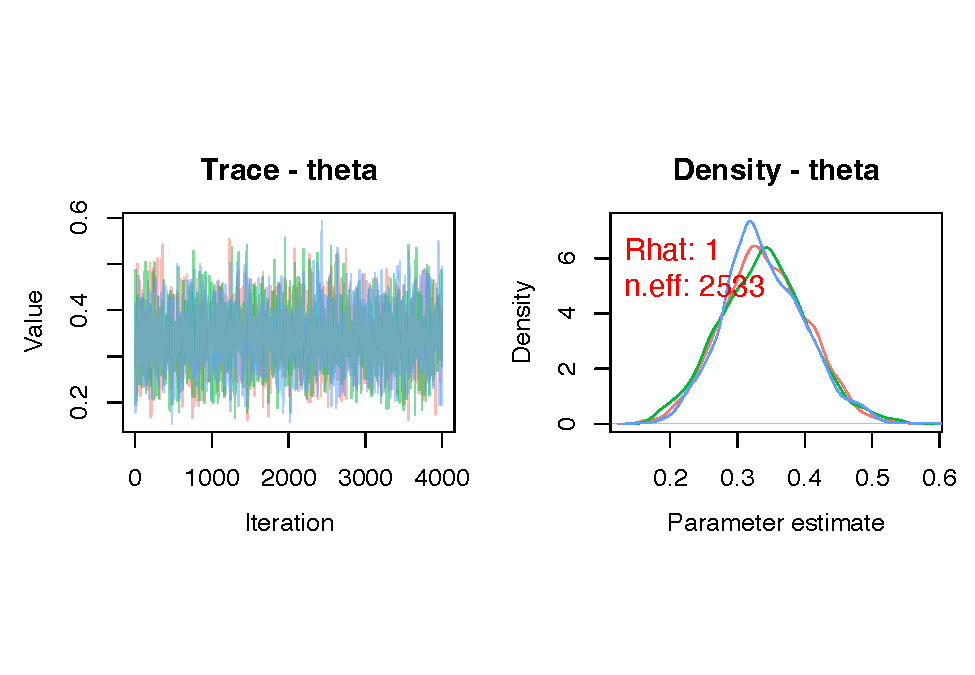
\includegraphics{banana-book_files/figure-latex/unnamed-chunk-48-1.pdf}

We calculated lifespan directly in our model with \texttt{lifespan\ \textless{}-\ -1/log(theta)}. But you can also calculate this quantity from outside NIMBLE. This is a nice by-product of using MCMC simulations: you can obtain the posterior distribution of any quantity that is function of your model parameters by applying this function to samples from the posterior distribution of these parameters. In our example, all you need is samples from the posterior distribution of \texttt{theta}, which we pool between the three chains with:

\begin{Shaded}
\begin{Highlighting}[]
\NormalTok{theta\_samples }\OtherTok{\textless{}{-}} \FunctionTok{c}\NormalTok{(mcmc.output}\SpecialCharTok{$}\NormalTok{chain1[,}\StringTok{\textquotesingle{}theta\textquotesingle{}}\NormalTok{], }
\NormalTok{                   mcmc.output}\SpecialCharTok{$}\NormalTok{chain2[,}\StringTok{\textquotesingle{}theta\textquotesingle{}}\NormalTok{],}
\NormalTok{                   mcmc.output}\SpecialCharTok{$}\NormalTok{chain3[,}\StringTok{\textquotesingle{}theta\textquotesingle{}}\NormalTok{])}
\end{Highlighting}
\end{Shaded}

To get samples from the posterior distribution of lifespan, we apply the function to calculate lifespan to the samples from the posterior distribution of survival:

\begin{Shaded}
\begin{Highlighting}[]
\NormalTok{lifespan }\OtherTok{\textless{}{-}} \SpecialCharTok{{-}}\DecValTok{1}\SpecialCharTok{/}\FunctionTok{log}\NormalTok{(theta\_samples)}
\end{Highlighting}
\end{Shaded}

As usual then, you can calculate the posterior mean and 95\% credible interval:

\begin{Shaded}
\begin{Highlighting}[]
\FunctionTok{mean}\NormalTok{(lifespan)}
\DocumentationTok{\#\# [1] 0.9398}
\FunctionTok{quantile}\NormalTok{(lifespan, }\AttributeTok{probs =} \FunctionTok{c}\NormalTok{(}\FloatTok{2.5}\NormalTok{, }\FloatTok{97.5}\NormalTok{)}\SpecialCharTok{/}\DecValTok{100}\NormalTok{)}
\DocumentationTok{\#\#   2.5\%  97.5\% }
\DocumentationTok{\#\# 0.6629 1.3194}
\end{Highlighting}
\end{Shaded}

You can also visualise the posterior distribution of lifespan:

\begin{Shaded}
\begin{Highlighting}[]
\NormalTok{lifespan }\SpecialCharTok{\%\textgreater{}\%}
  \FunctionTok{as\_tibble}\NormalTok{() }\SpecialCharTok{\%\textgreater{}\%}
  \FunctionTok{ggplot}\NormalTok{() }\SpecialCharTok{+}
  \FunctionTok{geom\_histogram}\NormalTok{(}\FunctionTok{aes}\NormalTok{(}\AttributeTok{x =}\NormalTok{ value), }\AttributeTok{color =} \StringTok{"white"}\NormalTok{) }\SpecialCharTok{+}
  \FunctionTok{labs}\NormalTok{(}\AttributeTok{x =} \StringTok{"lifespan"}\NormalTok{)}
\end{Highlighting}
\end{Shaded}

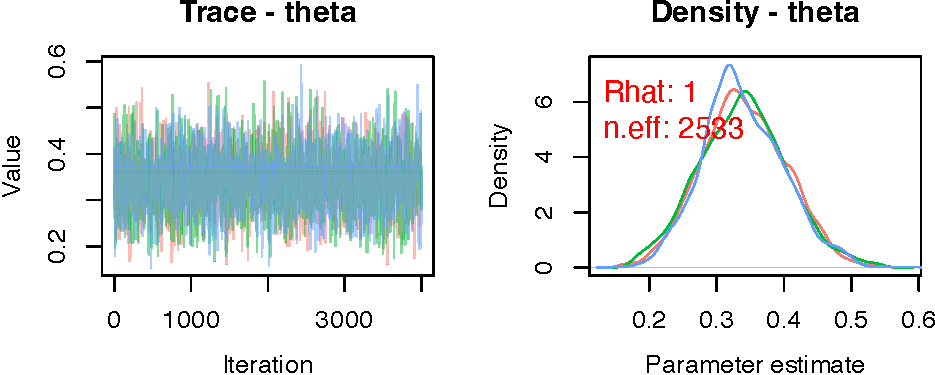
\includegraphics{banana-book_files/figure-latex/unnamed-chunk-52-1.pdf}

Now you're good to go. For convenience I have summarized the steps above in the box below. The NIMBLE workflow provided with \texttt{nimbleMCMC()} allows you to build models and make inference. This is what you can achieve with other software like WinBUGS or JAGS.

\textbf{NIMBLE workflow:}

\begin{Shaded}
\begin{Highlighting}[]
\CommentTok{\# model building}
\NormalTok{model }\OtherTok{\textless{}{-}} \FunctionTok{nimbleCode}\NormalTok{(\{}
  \CommentTok{\# likelihood}
\NormalTok{  survived }\SpecialCharTok{\textasciitilde{}} \FunctionTok{dbinom}\NormalTok{(theta, released)}
  \CommentTok{\# prior}
\NormalTok{  theta }\SpecialCharTok{\textasciitilde{}} \FunctionTok{dunif}\NormalTok{(}\DecValTok{0}\NormalTok{, }\DecValTok{1}\NormalTok{)}
  \CommentTok{\# derived quantity}
\NormalTok{  lifespan }\OtherTok{\textless{}{-}} \SpecialCharTok{{-}}\DecValTok{1}\SpecialCharTok{/}\FunctionTok{log}\NormalTok{(theta)}
\NormalTok{\})}
\CommentTok{\# read in data}
\NormalTok{my.data }\OtherTok{\textless{}{-}} \FunctionTok{list}\NormalTok{(}\AttributeTok{released =} \DecValTok{57}\NormalTok{, }\AttributeTok{survived =} \DecValTok{19}\NormalTok{)}
\CommentTok{\# specify parameters to monitor}
\NormalTok{parameters.to.save }\OtherTok{\textless{}{-}} \FunctionTok{c}\NormalTok{(}\StringTok{"theta"}\NormalTok{, }\StringTok{"lifespan"}\NormalTok{)}
\CommentTok{\# pick initial values}
\NormalTok{initial.values }\OtherTok{\textless{}{-}} \ControlFlowTok{function}\NormalTok{() }\FunctionTok{list}\NormalTok{(}\AttributeTok{theta =} \FunctionTok{runif}\NormalTok{(}\DecValTok{1}\NormalTok{,}\DecValTok{0}\NormalTok{,}\DecValTok{1}\NormalTok{))}
\CommentTok{\# specify MCMC details}
\NormalTok{n.iter }\OtherTok{\textless{}{-}} \DecValTok{5000}
\NormalTok{n.burnin }\OtherTok{\textless{}{-}} \DecValTok{1000}
\NormalTok{n.chains }\OtherTok{\textless{}{-}} \DecValTok{3}
\CommentTok{\# run NIMBLE}
\NormalTok{mcmc.output }\OtherTok{\textless{}{-}} \FunctionTok{nimbleMCMC}\NormalTok{(}\AttributeTok{code =}\NormalTok{ model,}
                          \AttributeTok{data =}\NormalTok{ my.data,}
                          \AttributeTok{inits =}\NormalTok{ initial.values,}
                          \AttributeTok{monitors =}\NormalTok{ parameters.to.save,}
                          \AttributeTok{niter =}\NormalTok{ n.iter,}
                          \AttributeTok{nburnin =}\NormalTok{ n.burnin,}
                          \AttributeTok{nchains =}\NormalTok{ n.chains)}
\CommentTok{\# calculate numerical summaries}
\FunctionTok{MCMCsummary}\NormalTok{(}\AttributeTok{object =}\NormalTok{ mcmc.output, }\AttributeTok{round =} \DecValTok{2}\NormalTok{)}
\CommentTok{\# visualize parameter posterior distribution}
\FunctionTok{MCMCplot}\NormalTok{(}\AttributeTok{object =}\NormalTok{ mcmc.output, }
         \AttributeTok{params =} \StringTok{\textquotesingle{}theta\textquotesingle{}}\NormalTok{)}
\CommentTok{\# check convergence}
\FunctionTok{MCMCtrace}\NormalTok{(}\AttributeTok{object =}\NormalTok{ mcmc.output,}
          \AttributeTok{pdf =} \ConstantTok{FALSE}\NormalTok{, }\CommentTok{\# no export to PDF}
          \AttributeTok{ind =} \ConstantTok{TRUE}\NormalTok{, }\CommentTok{\# separate density lines per chain}
          \AttributeTok{params =} \StringTok{"theta"}\NormalTok{)}
\end{Highlighting}
\end{Shaded}

But NIMBLE is more than just another MCMC engine. It provides a programming environment so that you have full control when building models and estimating parameters. NIMBLE allows you to write your own functions and distributions to build models, and to choose alternative MCMC samplers or code new ones. This flexibility often comes with faster convergence.

I have to be honest, learning these improvements over other software takes some reading and experimentation, and it might well be that you do not need to use any of these features. And it's fine. In the next sections, I cover some of this advanced material. You may skip these sections and go back to this material later if you need it.

\hypertarget{functions-in-nimble}{%
\section{Programming}\label{functions-in-nimble}}

In NIMBLE you can write and use your own functions, or use existing R or C/C++ functions. This allows you to customize models the way you want.

\hypertarget{nimble-functions}{%
\subsection{NIMBLE functions}\label{nimble-functions}}

NIMBLE provides \texttt{nimbleFunctions} for programming. A \texttt{nimbleFunction} is like an R function, plus it can be compiled for faster computation. Going back to our animal survival example, we can write a \texttt{nimbleFunction} to compute lifespan:

\begin{Shaded}
\begin{Highlighting}[]
\NormalTok{computeLifespan }\OtherTok{\textless{}{-}} \FunctionTok{nimbleFunction}\NormalTok{(}
    \AttributeTok{run =} \ControlFlowTok{function}\NormalTok{(}\AttributeTok{theta =} \FunctionTok{double}\NormalTok{(}\DecValTok{0}\NormalTok{)) \{ }\CommentTok{\# type declarations}
\NormalTok{        ans }\OtherTok{\textless{}{-}} \SpecialCharTok{{-}}\DecValTok{1}\SpecialCharTok{/}\FunctionTok{log}\NormalTok{(theta)}
        \FunctionTok{return}\NormalTok{(ans)}
        \FunctionTok{returnType}\NormalTok{(}\FunctionTok{double}\NormalTok{(}\DecValTok{0}\NormalTok{))  }\CommentTok{\# return type declaration}
\NormalTok{    \} )}
\end{Highlighting}
\end{Shaded}

Within the nimbleFunction, the \texttt{run} section gives the function to be executed. It is written in the NIMBLE language. The \texttt{theta\ =\ double(0)} and \texttt{returnType(double(0))} arguments tell NIMBLE that the input and output are single numeric values (scalars). Alternatively, \texttt{double(1)} and \texttt{double(2)} are for vectors and matrices, while \texttt{logical()}, \texttt{integer()} and \texttt{character()} are for logical, integer and character values.

You can use your \texttt{nimbleFunction} in R:

\begin{Shaded}
\begin{Highlighting}[]
\FunctionTok{computeLifespan}\NormalTok{(}\FloatTok{0.8}\NormalTok{)}
\DocumentationTok{\#\# [1] 4.481}
\end{Highlighting}
\end{Shaded}

You can compile it and use the C++ code for faster computation:

\begin{Shaded}
\begin{Highlighting}[]
\NormalTok{CcomputeLifespan }\OtherTok{\textless{}{-}} \FunctionTok{compileNimble}\NormalTok{(computeLifespan)}
\FunctionTok{CcomputeLifespan}\NormalTok{(}\FloatTok{0.8}\NormalTok{)}
\DocumentationTok{\#\# [1] 4.481}
\end{Highlighting}
\end{Shaded}

You can also use your \texttt{nimbleFunction} in a model:

\begin{Shaded}
\begin{Highlighting}[]
\NormalTok{model }\OtherTok{\textless{}{-}} \FunctionTok{nimbleCode}\NormalTok{(\{}
  \CommentTok{\# likelihood}
\NormalTok{  survived }\SpecialCharTok{\textasciitilde{}} \FunctionTok{dbinom}\NormalTok{(theta, released)}
  \CommentTok{\# prior}
\NormalTok{  theta }\SpecialCharTok{\textasciitilde{}} \FunctionTok{dunif}\NormalTok{(}\DecValTok{0}\NormalTok{, }\DecValTok{1}\NormalTok{)}
  \CommentTok{\# derived quantity}
\NormalTok{  lifespan }\OtherTok{\textless{}{-}} \FunctionTok{computeLifespan}\NormalTok{(theta)}
\NormalTok{\})}
\end{Highlighting}
\end{Shaded}

The rest of the workflow remains the same:

\begin{Shaded}
\begin{Highlighting}[]
\NormalTok{my.data }\OtherTok{\textless{}{-}} \FunctionTok{list}\NormalTok{(}\AttributeTok{survived =} \DecValTok{19}\NormalTok{, }\AttributeTok{released =} \DecValTok{57}\NormalTok{)}
\NormalTok{parameters.to.save }\OtherTok{\textless{}{-}} \FunctionTok{c}\NormalTok{(}\StringTok{"theta"}\NormalTok{, }\StringTok{"lifespan"}\NormalTok{)}
\NormalTok{initial.values }\OtherTok{\textless{}{-}} \ControlFlowTok{function}\NormalTok{() }\FunctionTok{list}\NormalTok{(}\AttributeTok{theta =} \FunctionTok{runif}\NormalTok{(}\DecValTok{1}\NormalTok{,}\DecValTok{0}\NormalTok{,}\DecValTok{1}\NormalTok{))}
\NormalTok{n.iter }\OtherTok{\textless{}{-}} \DecValTok{5000}
\NormalTok{n.burnin }\OtherTok{\textless{}{-}} \DecValTok{1000}
\NormalTok{n.chains }\OtherTok{\textless{}{-}} \DecValTok{3}
\NormalTok{mcmc.output }\OtherTok{\textless{}{-}} \FunctionTok{nimbleMCMC}\NormalTok{(}\AttributeTok{code =}\NormalTok{ model,}
                          \AttributeTok{data =}\NormalTok{ my.data,}
                          \AttributeTok{inits =}\NormalTok{ initial.values,}
                          \AttributeTok{monitors =}\NormalTok{ parameters.to.save,}
                          \AttributeTok{niter =}\NormalTok{ n.iter,}
                          \AttributeTok{nburnin =}\NormalTok{ n.burnin,}
                          \AttributeTok{nchains =}\NormalTok{ n.chains)}
\DocumentationTok{\#\# |{-}{-}{-}{-}{-}{-}{-}{-}{-}{-}{-}{-}{-}|{-}{-}{-}{-}{-}{-}{-}{-}{-}{-}{-}{-}{-}|{-}{-}{-}{-}{-}{-}{-}{-}{-}{-}{-}{-}{-}|{-}{-}{-}{-}{-}{-}{-}{-}{-}{-}{-}{-}{-}|}
\DocumentationTok{\#\# |{-}{-}{-}{-}{-}{-}{-}{-}{-}{-}{-}{-}{-}{-}{-}{-}{-}{-}{-}{-}{-}{-}{-}{-}{-}{-}{-}{-}{-}{-}{-}{-}{-}{-}{-}{-}{-}{-}{-}{-}{-}{-}{-}{-}{-}{-}{-}{-}{-}{-}{-}{-}{-}{-}{-}|}
\DocumentationTok{\#\# |{-}{-}{-}{-}{-}{-}{-}{-}{-}{-}{-}{-}{-}|{-}{-}{-}{-}{-}{-}{-}{-}{-}{-}{-}{-}{-}|{-}{-}{-}{-}{-}{-}{-}{-}{-}{-}{-}{-}{-}|{-}{-}{-}{-}{-}{-}{-}{-}{-}{-}{-}{-}{-}|}
\DocumentationTok{\#\# |{-}{-}{-}{-}{-}{-}{-}{-}{-}{-}{-}{-}{-}{-}{-}{-}{-}{-}{-}{-}{-}{-}{-}{-}{-}{-}{-}{-}{-}{-}{-}{-}{-}{-}{-}{-}{-}{-}{-}{-}{-}{-}{-}{-}{-}{-}{-}{-}{-}{-}{-}{-}{-}{-}{-}|}
\DocumentationTok{\#\# |{-}{-}{-}{-}{-}{-}{-}{-}{-}{-}{-}{-}{-}|{-}{-}{-}{-}{-}{-}{-}{-}{-}{-}{-}{-}{-}|{-}{-}{-}{-}{-}{-}{-}{-}{-}{-}{-}{-}{-}|{-}{-}{-}{-}{-}{-}{-}{-}{-}{-}{-}{-}{-}|}
\DocumentationTok{\#\# |{-}{-}{-}{-}{-}{-}{-}{-}{-}{-}{-}{-}{-}{-}{-}{-}{-}{-}{-}{-}{-}{-}{-}{-}{-}{-}{-}{-}{-}{-}{-}{-}{-}{-}{-}{-}{-}{-}{-}{-}{-}{-}{-}{-}{-}{-}{-}{-}{-}{-}{-}{-}{-}{-}{-}|}
\FunctionTok{MCMCsummary}\NormalTok{(}\AttributeTok{object =}\NormalTok{ mcmc.output, }\AttributeTok{round =} \DecValTok{2}\NormalTok{)}
\DocumentationTok{\#\#          mean   sd 2.5\%  50\% 97.5\% Rhat n.eff}
\DocumentationTok{\#\# lifespan 0.94 0.16 0.66 0.92  1.31    1  2593}
\DocumentationTok{\#\# theta    0.34 0.06 0.22 0.34  0.47    1  2652}
\end{Highlighting}
\end{Shaded}

With \texttt{nimbleFunctions}, you can mimic basic R syntax, do linear algebra (e.g.~compute eigenvalues), operate on vectors and matrices (e.g.~inverse a matrix), use logical operators (e.g.~and/or) and flow control (e.g.~if-else). There is also a long list of common and less common distributions that can be used with \texttt{nimbleFunctions}.

To learn everything you need to know on writing \texttt{nimbleFunctions}, make sure to read chapter 11 of the NIMBLE manual at \url{https://r-nimble.org/html_manual/cha-RCfunctions.html\#cha-RCfunctions}.

\hypertarget{callrfninnimble}{%
\subsection{Calling R/C++ functions}\label{callrfninnimble}}

If you're like me, and too lazy to write your own functions, you can rely on the scientific community and use existing C, C++ or R code. The trick is to write a \texttt{nimbleFunction} that wraps access to that code which can then be used by NIMBLE. As an example, imagine you'd like to use an R function \texttt{myfunction()}, either a function you wrote yourself, or a function available in your favorite R package:

\begin{Shaded}
\begin{Highlighting}[]
\NormalTok{myfunction }\OtherTok{\textless{}{-}} \ControlFlowTok{function}\NormalTok{(x) \{}
  \SpecialCharTok{{-}}\DecValTok{1}\SpecialCharTok{/}\FunctionTok{log}\NormalTok{(x)}
\NormalTok{\}}
\end{Highlighting}
\end{Shaded}

Now wrap this function using \texttt{nimbleRcall()} or \texttt{nimbleExternalCall()} for a C or C++ function:

\begin{Shaded}
\begin{Highlighting}[]
\NormalTok{Rmyfunction }\OtherTok{\textless{}{-}} \FunctionTok{nimbleRcall}\NormalTok{(}\AttributeTok{prototype =} \ControlFlowTok{function}\NormalTok{(}\AttributeTok{x =} \FunctionTok{double}\NormalTok{(}\DecValTok{0}\NormalTok{))\{\}, }
                           \AttributeTok{Rfun =} \StringTok{\textquotesingle{}myfunction\textquotesingle{}}\NormalTok{,}
                           \AttributeTok{returnType =} \FunctionTok{double}\NormalTok{(}\DecValTok{0}\NormalTok{))}
\end{Highlighting}
\end{Shaded}

In the call to \texttt{nimbleRcall()} above, the argument \texttt{prototype} specifies inputs (a single numeric value \texttt{double(0)}) of the R function \texttt{Rfun} that generates outputs \texttt{returnType} (a single numeric value \texttt{double(0)}).

Now you can call your R function from a model (or any \texttt{nimbleFunctions}):

\begin{Shaded}
\begin{Highlighting}[]
\NormalTok{model }\OtherTok{\textless{}{-}} \FunctionTok{nimbleCode}\NormalTok{(\{}
  \CommentTok{\# likelihood}
\NormalTok{  survived }\SpecialCharTok{\textasciitilde{}} \FunctionTok{dbinom}\NormalTok{(theta, released)}
  \CommentTok{\# prior}
\NormalTok{  theta }\SpecialCharTok{\textasciitilde{}} \FunctionTok{dunif}\NormalTok{(}\DecValTok{0}\NormalTok{, }\DecValTok{1}\NormalTok{)}
\NormalTok{  lifespan }\OtherTok{\textless{}{-}} \FunctionTok{Rmyfunction}\NormalTok{(theta)}
\NormalTok{\})}
\end{Highlighting}
\end{Shaded}

The rest of the workflow remains the same:

\begin{Shaded}
\begin{Highlighting}[]
\NormalTok{my.data }\OtherTok{\textless{}{-}} \FunctionTok{list}\NormalTok{(}\AttributeTok{survived =} \DecValTok{19}\NormalTok{, }\AttributeTok{released =} \DecValTok{57}\NormalTok{)}
\NormalTok{parameters.to.save }\OtherTok{\textless{}{-}} \FunctionTok{c}\NormalTok{(}\StringTok{"theta"}\NormalTok{, }\StringTok{"lifespan"}\NormalTok{)}
\NormalTok{initial.values }\OtherTok{\textless{}{-}} \ControlFlowTok{function}\NormalTok{() }\FunctionTok{list}\NormalTok{(}\AttributeTok{theta =} \FunctionTok{runif}\NormalTok{(}\DecValTok{1}\NormalTok{,}\DecValTok{0}\NormalTok{,}\DecValTok{1}\NormalTok{))}
\NormalTok{n.iter }\OtherTok{\textless{}{-}} \DecValTok{5000}
\NormalTok{n.burnin }\OtherTok{\textless{}{-}} \DecValTok{1000}
\NormalTok{n.chains }\OtherTok{\textless{}{-}} \DecValTok{3}
\NormalTok{mcmc.output }\OtherTok{\textless{}{-}} \FunctionTok{nimbleMCMC}\NormalTok{(}\AttributeTok{code =}\NormalTok{ model,}
                          \AttributeTok{data =}\NormalTok{ my.data,}
                          \AttributeTok{inits =}\NormalTok{ initial.values,}
                          \AttributeTok{monitors =}\NormalTok{ parameters.to.save,}
                          \AttributeTok{niter =}\NormalTok{ n.iter,}
                          \AttributeTok{nburnin =}\NormalTok{ n.burnin,}
                          \AttributeTok{nchains =}\NormalTok{ n.chains)}
\DocumentationTok{\#\# |{-}{-}{-}{-}{-}{-}{-}{-}{-}{-}{-}{-}{-}|{-}{-}{-}{-}{-}{-}{-}{-}{-}{-}{-}{-}{-}|{-}{-}{-}{-}{-}{-}{-}{-}{-}{-}{-}{-}{-}|{-}{-}{-}{-}{-}{-}{-}{-}{-}{-}{-}{-}{-}|}
\DocumentationTok{\#\# |{-}{-}{-}{-}{-}{-}{-}{-}{-}{-}{-}{-}{-}{-}{-}{-}{-}{-}{-}{-}{-}{-}{-}{-}{-}{-}{-}{-}{-}{-}{-}{-}{-}{-}{-}{-}{-}{-}{-}{-}{-}{-}{-}{-}{-}{-}{-}{-}{-}{-}{-}{-}{-}{-}{-}|}
\DocumentationTok{\#\# |{-}{-}{-}{-}{-}{-}{-}{-}{-}{-}{-}{-}{-}|{-}{-}{-}{-}{-}{-}{-}{-}{-}{-}{-}{-}{-}|{-}{-}{-}{-}{-}{-}{-}{-}{-}{-}{-}{-}{-}|{-}{-}{-}{-}{-}{-}{-}{-}{-}{-}{-}{-}{-}|}
\DocumentationTok{\#\# |{-}{-}{-}{-}{-}{-}{-}{-}{-}{-}{-}{-}{-}{-}{-}{-}{-}{-}{-}{-}{-}{-}{-}{-}{-}{-}{-}{-}{-}{-}{-}{-}{-}{-}{-}{-}{-}{-}{-}{-}{-}{-}{-}{-}{-}{-}{-}{-}{-}{-}{-}{-}{-}{-}{-}|}
\DocumentationTok{\#\# |{-}{-}{-}{-}{-}{-}{-}{-}{-}{-}{-}{-}{-}|{-}{-}{-}{-}{-}{-}{-}{-}{-}{-}{-}{-}{-}|{-}{-}{-}{-}{-}{-}{-}{-}{-}{-}{-}{-}{-}|{-}{-}{-}{-}{-}{-}{-}{-}{-}{-}{-}{-}{-}|}
\DocumentationTok{\#\# |{-}{-}{-}{-}{-}{-}{-}{-}{-}{-}{-}{-}{-}{-}{-}{-}{-}{-}{-}{-}{-}{-}{-}{-}{-}{-}{-}{-}{-}{-}{-}{-}{-}{-}{-}{-}{-}{-}{-}{-}{-}{-}{-}{-}{-}{-}{-}{-}{-}{-}{-}{-}{-}{-}{-}|}
\FunctionTok{MCMCsummary}\NormalTok{(}\AttributeTok{object =}\NormalTok{ mcmc.output, }\AttributeTok{round =} \DecValTok{2}\NormalTok{)}
\DocumentationTok{\#\#          mean   sd 2.5\%  50\% 97.5\% Rhat n.eff}
\DocumentationTok{\#\# lifespan 0.94 0.16 0.68 0.92  1.29    1  2597}
\DocumentationTok{\#\# theta    0.34 0.06 0.23 0.34  0.46    1  2643}
\end{Highlighting}
\end{Shaded}

Evaluating an R function from within NIMBLE slows MCMC sampling down, but if you can live with it, the cost is easily offset by the convenience of being able to use existing R functions.

Another advantage of using \texttt{nimbleRcall()} (or \texttt{nimbleExternalCall()}) is that you can keep large objects out of your model, so that NIMBLE does not have to handle them in MCMC sampling. These objects should be constants and not change when you run NIMBLE. Letting R manipulating these objects will save you time, usually more than the time you lose by calling R from within NIMBLE.

\hypertarget{user-defined-distributions}{%
\subsection{User-defined distributions}\label{user-defined-distributions}}

With \texttt{nimbleFunctions} you can provide user-defined distributions to NIMBLE. You need to write functions for density (\texttt{d}) and simulation (\texttt{r}) for your distribution. As an example, we write our own binomial distribution:

\begin{Shaded}
\begin{Highlighting}[]
\CommentTok{\# density}
\NormalTok{dmybinom }\OtherTok{\textless{}{-}} \FunctionTok{nimbleFunction}\NormalTok{(}
  \AttributeTok{run =} \ControlFlowTok{function}\NormalTok{(}\AttributeTok{x =} \FunctionTok{double}\NormalTok{(}\DecValTok{0}\NormalTok{), }
                 \AttributeTok{size =} \FunctionTok{double}\NormalTok{(}\DecValTok{0}\NormalTok{), }
                 \AttributeTok{prob =} \FunctionTok{double}\NormalTok{(}\DecValTok{0}\NormalTok{), }
                 \AttributeTok{log =} \FunctionTok{integer}\NormalTok{(}\DecValTok{0}\NormalTok{, }\AttributeTok{default =} \DecValTok{1}\NormalTok{)) \{}
    \FunctionTok{returnType}\NormalTok{(}\FunctionTok{double}\NormalTok{(}\DecValTok{0}\NormalTok{))}
    \CommentTok{\# compute binomial coefficient }
\NormalTok{    lchoose }\OtherTok{\textless{}{-}} \FunctionTok{lfactorial}\NormalTok{(size) }\SpecialCharTok{{-}} \FunctionTok{lfactorial}\NormalTok{(x) }\SpecialCharTok{{-}} \FunctionTok{lfactorial}\NormalTok{(size }\SpecialCharTok{{-}}\NormalTok{ x)}
    \CommentTok{\# binomial density function}
\NormalTok{    logProb }\OtherTok{\textless{}{-}}\NormalTok{ lchoose }\SpecialCharTok{+}\NormalTok{ x }\SpecialCharTok{*} \FunctionTok{log}\NormalTok{(prob) }\SpecialCharTok{+}\NormalTok{ (size }\SpecialCharTok{{-}}\NormalTok{ x) }\SpecialCharTok{*} \FunctionTok{log}\NormalTok{(}\DecValTok{1} \SpecialCharTok{{-}}\NormalTok{ prob)}
    \ControlFlowTok{if}\NormalTok{(log) }\FunctionTok{return}\NormalTok{(logProb)}
    \ControlFlowTok{else} \FunctionTok{return}\NormalTok{(}\FunctionTok{exp}\NormalTok{(logProb)) }
\NormalTok{  \})}
\CommentTok{\# simulation using the coin flip method (p. 524 in Devroye 1986)}
\NormalTok{rmybinom }\OtherTok{\textless{}{-}} \FunctionTok{nimbleFunction}\NormalTok{(}
  \AttributeTok{run =} \ControlFlowTok{function}\NormalTok{(}\AttributeTok{n =} \FunctionTok{integer}\NormalTok{(}\DecValTok{0}\NormalTok{, }\AttributeTok{default =} \DecValTok{1}\NormalTok{),}
                 \AttributeTok{size =} \FunctionTok{double}\NormalTok{(}\DecValTok{0}\NormalTok{),}
                 \AttributeTok{prob =} \FunctionTok{double}\NormalTok{(}\DecValTok{0}\NormalTok{)) \{}
    \FunctionTok{returnType}\NormalTok{(}\FunctionTok{double}\NormalTok{(}\DecValTok{0}\NormalTok{))}
\NormalTok{    x }\OtherTok{\textless{}{-}} \DecValTok{0}
\NormalTok{    y }\OtherTok{\textless{}{-}} \FunctionTok{runif}\NormalTok{(}\AttributeTok{n =}\NormalTok{ size, }\AttributeTok{min =} \DecValTok{0}\NormalTok{, }\AttributeTok{max =} \DecValTok{1}\NormalTok{)}
    \ControlFlowTok{for}\NormalTok{ (j }\ControlFlowTok{in} \DecValTok{1}\SpecialCharTok{:}\NormalTok{size)\{}
      \ControlFlowTok{if}\NormalTok{ (y[j] }\SpecialCharTok{\textless{}}\NormalTok{ prob)\{}
\NormalTok{        x }\OtherTok{\textless{}{-}}\NormalTok{ x }\SpecialCharTok{+} \DecValTok{1}
\NormalTok{      \}}\ControlFlowTok{else}\NormalTok{\{}
\NormalTok{        x }\OtherTok{\textless{}{-}}\NormalTok{ x}
\NormalTok{      \}}
\NormalTok{    \}}
    \FunctionTok{return}\NormalTok{(x)    }
\NormalTok{  \})}
\end{Highlighting}
\end{Shaded}

You need to define the \texttt{nimbleFunctions} in R's global environment for them to be accessed:

\begin{Shaded}
\begin{Highlighting}[]
\FunctionTok{assign}\NormalTok{(}\StringTok{\textquotesingle{}dmybinom\textquotesingle{}}\NormalTok{, dmybinom, .GlobalEnv)}
\FunctionTok{assign}\NormalTok{(}\StringTok{\textquotesingle{}rmybinom\textquotesingle{}}\NormalTok{, rmybinom, .GlobalEnv)}
\end{Highlighting}
\end{Shaded}

You can try out your function and simulate a random value from a binomial distribution with size 5 and probability 0.1:

\begin{Shaded}
\begin{Highlighting}[]
\FunctionTok{rmybinom}\NormalTok{(}\AttributeTok{n =} \DecValTok{1}\NormalTok{, }\AttributeTok{size =} \DecValTok{5}\NormalTok{, }\AttributeTok{prob =} \FloatTok{0.1}\NormalTok{)}
\DocumentationTok{\#\# [1] 0}
\end{Highlighting}
\end{Shaded}

All set. You can run your workflow:

\begin{Shaded}
\begin{Highlighting}[]
\NormalTok{model }\OtherTok{\textless{}{-}} \FunctionTok{nimbleCode}\NormalTok{(\{}
 \CommentTok{\# likelihood}
\NormalTok{ survived }\SpecialCharTok{\textasciitilde{}} \FunctionTok{dmybinom}\NormalTok{(}\AttributeTok{prob =}\NormalTok{ theta, }\AttributeTok{size =}\NormalTok{ released)}
 \CommentTok{\# prior}
\NormalTok{ theta }\SpecialCharTok{\textasciitilde{}} \FunctionTok{dunif}\NormalTok{(}\DecValTok{0}\NormalTok{, }\DecValTok{1}\NormalTok{)}
\NormalTok{\})}
\NormalTok{my.data }\OtherTok{\textless{}{-}} \FunctionTok{list}\NormalTok{(}\AttributeTok{released =} \DecValTok{57}\NormalTok{, }\AttributeTok{survived =} \DecValTok{19}\NormalTok{)}
\NormalTok{initial.values }\OtherTok{\textless{}{-}} \ControlFlowTok{function}\NormalTok{() }\FunctionTok{list}\NormalTok{(}\AttributeTok{theta =} \FunctionTok{runif}\NormalTok{(}\DecValTok{1}\NormalTok{,}\DecValTok{0}\NormalTok{,}\DecValTok{1}\NormalTok{))}
\NormalTok{n.iter }\OtherTok{\textless{}{-}} \DecValTok{5000}
\NormalTok{n.burnin }\OtherTok{\textless{}{-}} \DecValTok{1000}
\NormalTok{n.chains }\OtherTok{\textless{}{-}} \DecValTok{3}
\NormalTok{mcmc.output }\OtherTok{\textless{}{-}} \FunctionTok{nimbleMCMC}\NormalTok{(}\AttributeTok{code =}\NormalTok{ model,}
 \AttributeTok{data =}\NormalTok{ my.data,}
 \AttributeTok{inits =}\NormalTok{ initial.values,}
 \AttributeTok{niter =}\NormalTok{ n.iter,}
 \AttributeTok{nburnin =}\NormalTok{ n.burnin,}
 \AttributeTok{nchains =}\NormalTok{ n.chains)}
\DocumentationTok{\#\# |{-}{-}{-}{-}{-}{-}{-}{-}{-}{-}{-}{-}{-}|{-}{-}{-}{-}{-}{-}{-}{-}{-}{-}{-}{-}{-}|{-}{-}{-}{-}{-}{-}{-}{-}{-}{-}{-}{-}{-}|{-}{-}{-}{-}{-}{-}{-}{-}{-}{-}{-}{-}{-}|}
\DocumentationTok{\#\# |{-}{-}{-}{-}{-}{-}{-}{-}{-}{-}{-}{-}{-}{-}{-}{-}{-}{-}{-}{-}{-}{-}{-}{-}{-}{-}{-}{-}{-}{-}{-}{-}{-}{-}{-}{-}{-}{-}{-}{-}{-}{-}{-}{-}{-}{-}{-}{-}{-}{-}{-}{-}{-}{-}{-}|}
\DocumentationTok{\#\# |{-}{-}{-}{-}{-}{-}{-}{-}{-}{-}{-}{-}{-}|{-}{-}{-}{-}{-}{-}{-}{-}{-}{-}{-}{-}{-}|{-}{-}{-}{-}{-}{-}{-}{-}{-}{-}{-}{-}{-}|{-}{-}{-}{-}{-}{-}{-}{-}{-}{-}{-}{-}{-}|}
\DocumentationTok{\#\# |{-}{-}{-}{-}{-}{-}{-}{-}{-}{-}{-}{-}{-}{-}{-}{-}{-}{-}{-}{-}{-}{-}{-}{-}{-}{-}{-}{-}{-}{-}{-}{-}{-}{-}{-}{-}{-}{-}{-}{-}{-}{-}{-}{-}{-}{-}{-}{-}{-}{-}{-}{-}{-}{-}{-}|}
\DocumentationTok{\#\# |{-}{-}{-}{-}{-}{-}{-}{-}{-}{-}{-}{-}{-}|{-}{-}{-}{-}{-}{-}{-}{-}{-}{-}{-}{-}{-}|{-}{-}{-}{-}{-}{-}{-}{-}{-}{-}{-}{-}{-}|{-}{-}{-}{-}{-}{-}{-}{-}{-}{-}{-}{-}{-}|}
\DocumentationTok{\#\# |{-}{-}{-}{-}{-}{-}{-}{-}{-}{-}{-}{-}{-}{-}{-}{-}{-}{-}{-}{-}{-}{-}{-}{-}{-}{-}{-}{-}{-}{-}{-}{-}{-}{-}{-}{-}{-}{-}{-}{-}{-}{-}{-}{-}{-}{-}{-}{-}{-}{-}{-}{-}{-}{-}{-}|}
\FunctionTok{MCMCsummary}\NormalTok{(mcmc.output)}
\DocumentationTok{\#\#       mean      sd   2.5\%    50\%  97.5\% Rhat n.eff}
\DocumentationTok{\#\# theta 0.34 0.05976 0.2286 0.3378 0.4598    1  2970}
\end{Highlighting}
\end{Shaded}

Having \texttt{nimbleFunctions} offers infinite possibilities to customize your models and algorithms. Besides what we covered already, you can write your own samplers. We will see an example in a minute, but I first need to tell you more about the NIMBLE workflow.

\hypertarget{under-the-hood}{%
\section{Under the hood}\label{under-the-hood}}

So far, you have used \texttt{nimbleMCMC()} which runs the default MCMC workflow. This is perfecly fine for most applications. However, in some situations you need to customize the MCMC samplers to improve or fasten convergence. NIMBLE allows you to look under the hood by using a detailed workflow in several steps: \texttt{nimbleModel()}, \texttt{configureMCMC()}, \texttt{buildMCMC()}, \texttt{compileNimble()} and \texttt{runMCMC()}. Note that \texttt{nimbleMCMC()} does all of this at once.

We write the model code, read in data and pick initial values as before:

\begin{Shaded}
\begin{Highlighting}[]
\NormalTok{model }\OtherTok{\textless{}{-}} \FunctionTok{nimbleCode}\NormalTok{(\{}
  \CommentTok{\# likelihood}
\NormalTok{  survived }\SpecialCharTok{\textasciitilde{}} \FunctionTok{dbinom}\NormalTok{(theta, released)}
  \CommentTok{\# prior}
\NormalTok{  theta }\SpecialCharTok{\textasciitilde{}} \FunctionTok{dunif}\NormalTok{(}\DecValTok{0}\NormalTok{, }\DecValTok{1}\NormalTok{)}
  \CommentTok{\# derived quantity}
\NormalTok{  lifespan }\OtherTok{\textless{}{-}} \SpecialCharTok{{-}}\DecValTok{1}\SpecialCharTok{/}\FunctionTok{log}\NormalTok{(theta)}
\NormalTok{\})}
\NormalTok{my.data }\OtherTok{\textless{}{-}} \FunctionTok{list}\NormalTok{(}\AttributeTok{survived =} \DecValTok{19}\NormalTok{, }\AttributeTok{released =} \DecValTok{57}\NormalTok{)}
\NormalTok{initial.values }\OtherTok{\textless{}{-}} \FunctionTok{list}\NormalTok{(}\AttributeTok{theta =} \FloatTok{0.5}\NormalTok{)}
\end{Highlighting}
\end{Shaded}

First step is to create the model as an R object (uncompiled model) with \texttt{nimbleModel()}:

\begin{Shaded}
\begin{Highlighting}[]
\NormalTok{survival }\OtherTok{\textless{}{-}} \FunctionTok{nimbleModel}\NormalTok{(}\AttributeTok{code =}\NormalTok{ model,}
                        \AttributeTok{data =}\NormalTok{ my.data,}
                        \AttributeTok{inits =}\NormalTok{ initial.values)}
\end{Highlighting}
\end{Shaded}

You can look at its nodes:

\begin{Shaded}
\begin{Highlighting}[]
\NormalTok{survival}\SpecialCharTok{$}\FunctionTok{getNodeNames}\NormalTok{()}
\DocumentationTok{\#\# [1] "theta"    "lifespan" "survived"}
\end{Highlighting}
\end{Shaded}

You can look at the values stored at each node:

\begin{Shaded}
\begin{Highlighting}[]
\NormalTok{survival}\SpecialCharTok{$}\NormalTok{theta}
\DocumentationTok{\#\# [1] 0.5}
\NormalTok{survival}\SpecialCharTok{$}\NormalTok{survived}
\DocumentationTok{\#\# [1] 19}
\NormalTok{survival}\SpecialCharTok{$}\NormalTok{lifespan }
\DocumentationTok{\#\# [1] 1.443}
\CommentTok{\# this is {-}1/log(0.5)}
\end{Highlighting}
\end{Shaded}

We can also calculate the log-likelihood at the initial value for \texttt{theta}:

\begin{Shaded}
\begin{Highlighting}[]
\NormalTok{survival}\SpecialCharTok{$}\FunctionTok{calculate}\NormalTok{()}
\DocumentationTok{\#\# [1] {-}5.422}
\CommentTok{\# this is dbinom(x = 19, size = 57, prob = 0.5, log = TRUE)}
\end{Highlighting}
\end{Shaded}

The ability in NIMBLE to access the nodes of your model and to evaluate the model likelihood can help you in identifying bugs in your code. \textbf{Give example? Provide negative initial value for theta, or released in data \textless{} survived.}

You can obtain the graph of the model as in Figure \ref{fig:dag-survival} with:

\begin{Shaded}
\begin{Highlighting}[]
\NormalTok{survival}\SpecialCharTok{$}\FunctionTok{plotGraph}\NormalTok{()}
\end{Highlighting}
\end{Shaded}

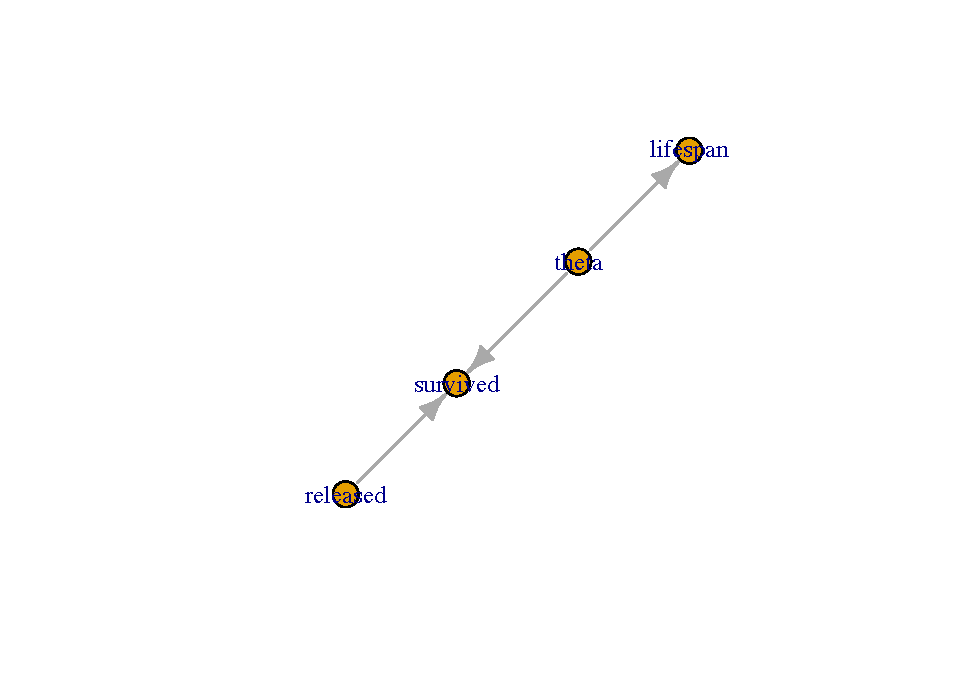
\includegraphics{banana-book_files/figure-latex/unnamed-chunk-72-1.pdf}

Second we compile the model with \texttt{compileNimble()}:

\begin{Shaded}
\begin{Highlighting}[]
\NormalTok{Csurvival }\OtherTok{\textless{}{-}} \FunctionTok{compileNimble}\NormalTok{(survival)}
\end{Highlighting}
\end{Shaded}

With \texttt{compileNimble()}, the C++ code is generated, compiled and loaded back into R so that it can be used in R (compiled model):

\begin{Shaded}
\begin{Highlighting}[]
\NormalTok{Csurvival}\SpecialCharTok{$}\NormalTok{theta}
\DocumentationTok{\#\# [1] 0.5}
\end{Highlighting}
\end{Shaded}

Now you have two versions of the model, \texttt{survival} is in R and \texttt{Csurvival} in C++. Being able to separate the steps of model building and parameter estimation is a strength of NIMBLE. This gives you a lot of flexibility at both steps. For example, imagine you would like to fit your model with maximum likelihood, then you can do it by wrapping your model in an R function that gets the likelihood and maximise this function. Using the C version of the model, you can write:

\begin{Shaded}
\begin{Highlighting}[]
\CommentTok{\# function for negative log{-}likelihood to minimize}
\NormalTok{f }\OtherTok{\textless{}{-}} \ControlFlowTok{function}\NormalTok{(par) \{}
\NormalTok{    Csurvival[[}\StringTok{\textquotesingle{}theta\textquotesingle{}}\NormalTok{]] }\OtherTok{\textless{}{-}}\NormalTok{ par }\CommentTok{\# assign par to theta }
\NormalTok{    ll }\OtherTok{\textless{}{-}}\NormalTok{ Csurvival}\SpecialCharTok{$}\FunctionTok{calculate}\NormalTok{() }\CommentTok{\# update log{-}likelihood with par value}
    \FunctionTok{return}\NormalTok{(}\SpecialCharTok{{-}}\NormalTok{ll) }\CommentTok{\# return negative log{-}likelihood}
\NormalTok{\}}
\CommentTok{\# evaluate function at 0.5 and 0.9}
\FunctionTok{f}\NormalTok{(}\FloatTok{0.5}\NormalTok{)}
\DocumentationTok{\#\# [1] 5.422}
\FunctionTok{f}\NormalTok{(}\FloatTok{0.9}\NormalTok{)}
\DocumentationTok{\#\# [1] 55.41}
\CommentTok{\# minimize function}
\NormalTok{out }\OtherTok{\textless{}{-}} \FunctionTok{optimize}\NormalTok{(f, }\AttributeTok{interval =} \FunctionTok{c}\NormalTok{(}\DecValTok{0}\NormalTok{,}\DecValTok{1}\NormalTok{))}
\FunctionTok{round}\NormalTok{(out}\SpecialCharTok{$}\NormalTok{minimum, }\DecValTok{2}\NormalTok{)}
\DocumentationTok{\#\# [1] 0.33}
\end{Highlighting}
\end{Shaded}

By maximising the likelihood (or minimising the negative log-likelihood), you obtain the maximum likelihood estimate of animal survival, which is exactly 19 surviving animals over 57 released animals or 0.33.

Third we create a MCMC configuration for our model with \texttt{configureMCMC()}:

\begin{Shaded}
\begin{Highlighting}[]
\NormalTok{survivalConf }\OtherTok{\textless{}{-}} \FunctionTok{configureMCMC}\NormalTok{(survival)}
\DocumentationTok{\#\# ===== Monitors =====}
\DocumentationTok{\#\# thin = 1: theta}
\DocumentationTok{\#\# ===== Samplers =====}
\DocumentationTok{\#\# RW sampler (1)}
\DocumentationTok{\#\#   {-} theta}
\end{Highlighting}
\end{Shaded}

This steps tells you the nodes that are monitored by default, and the MCMC samplers than have been assigned to them. Here \texttt{theta} is monitored, and samples from its posterior distribution are simulated with a random walk sampler similar to the Metropolis sampler we coded in the previous chapter in Section \ref{metropolis-algorithm}.

To monitor \texttt{lifespan} in addition to \texttt{theta}, you write:

\begin{Shaded}
\begin{Highlighting}[]
\NormalTok{survivalConf}\SpecialCharTok{$}\FunctionTok{addMonitors}\NormalTok{(}\FunctionTok{c}\NormalTok{(}\StringTok{"lifespan"}\NormalTok{))}
\DocumentationTok{\#\# thin = 1: lifespan, theta}
\NormalTok{survivalConf}
\DocumentationTok{\#\# ===== Monitors =====}
\DocumentationTok{\#\# thin = 1: lifespan, theta}
\DocumentationTok{\#\# ===== Samplers =====}
\DocumentationTok{\#\# RW sampler (1)}
\DocumentationTok{\#\#   {-} theta}
\end{Highlighting}
\end{Shaded}

Third, we create a MCMC function with \texttt{buildMCMC()} and compile it with \texttt{compileNimble()}:

\begin{Shaded}
\begin{Highlighting}[]
\NormalTok{survivalMCMC }\OtherTok{\textless{}{-}} \FunctionTok{buildMCMC}\NormalTok{(survivalConf)}
\NormalTok{CsurvivalMCMC }\OtherTok{\textless{}{-}} \FunctionTok{compileNimble}\NormalTok{(survivalMCMC, }\AttributeTok{project =}\NormalTok{ survival)}
\end{Highlighting}
\end{Shaded}

Note that models and \texttt{nimbleFunctions} need to be compiled before they can be used to specify a project.

Fourth, we run NIMBLE with \texttt{runMCMC()}:

\begin{Shaded}
\begin{Highlighting}[]
\NormalTok{n.iter }\OtherTok{\textless{}{-}} \DecValTok{5000}
\NormalTok{n.burnin }\OtherTok{\textless{}{-}} \DecValTok{1000}
\NormalTok{samples }\OtherTok{\textless{}{-}} \FunctionTok{runMCMC}\NormalTok{(}\AttributeTok{mcmc =}\NormalTok{ CsurvivalMCMC, }
                   \AttributeTok{niter =}\NormalTok{ n.iter,}
                   \AttributeTok{nburnin =}\NormalTok{ n.burnin)}
\DocumentationTok{\#\# |{-}{-}{-}{-}{-}{-}{-}{-}{-}{-}{-}{-}{-}|{-}{-}{-}{-}{-}{-}{-}{-}{-}{-}{-}{-}{-}|{-}{-}{-}{-}{-}{-}{-}{-}{-}{-}{-}{-}{-}|{-}{-}{-}{-}{-}{-}{-}{-}{-}{-}{-}{-}{-}|}
\DocumentationTok{\#\# |{-}{-}{-}{-}{-}{-}{-}{-}{-}{-}{-}{-}{-}{-}{-}{-}{-}{-}{-}{-}{-}{-}{-}{-}{-}{-}{-}{-}{-}{-}{-}{-}{-}{-}{-}{-}{-}{-}{-}{-}{-}{-}{-}{-}{-}{-}{-}{-}{-}{-}{-}{-}{-}{-}{-}|}
\end{Highlighting}
\end{Shaded}

We run a single chain but \texttt{runMCMC()} allows you to use multiple chains as with \texttt{nimbleMCMC()}.

You can look into \texttt{samples} which contains values simulated from the posterior distribution of the parameters we monitor:

\begin{Shaded}
\begin{Highlighting}[]
\FunctionTok{head}\NormalTok{(samples)}
\DocumentationTok{\#\#      lifespan  theta}
\DocumentationTok{\#\# [1,]   0.9093 0.3330}
\DocumentationTok{\#\# [2,]   0.9093 0.3330}
\DocumentationTok{\#\# [3,]   0.9093 0.3330}
\DocumentationTok{\#\# [4,]   1.2095 0.4374}
\DocumentationTok{\#\# [5,]   1.2095 0.4374}
\DocumentationTok{\#\# [6,]   1.1835 0.4296}
\end{Highlighting}
\end{Shaded}

From here, you can obtain numerical summaries with \texttt{samplesSummary()}:

\begin{Shaded}
\begin{Highlighting}[]
\FunctionTok{samplesSummary}\NormalTok{(samples)}
\DocumentationTok{\#\#            Mean Median St.Dev. 95\%CI\_low 95\%CI\_upp}
\DocumentationTok{\#\# lifespan 0.9357 0.9194 0.16117    0.6831    1.2969}
\DocumentationTok{\#\# theta    0.3386 0.3370 0.06128    0.2313    0.4625}
\end{Highlighting}
\end{Shaded}

I have summarized the steps above in the box below.

\textbf{Detailed NIMBLE workflow:}

\begin{Shaded}
\begin{Highlighting}[]
\CommentTok{\# model building}
\NormalTok{model }\OtherTok{\textless{}{-}} \FunctionTok{nimbleCode}\NormalTok{(\{}
  \CommentTok{\# likelihood}
\NormalTok{  survived }\SpecialCharTok{\textasciitilde{}} \FunctionTok{dbinom}\NormalTok{(theta, released)}
  \CommentTok{\# prior}
\NormalTok{  theta }\SpecialCharTok{\textasciitilde{}} \FunctionTok{dunif}\NormalTok{(}\DecValTok{0}\NormalTok{, }\DecValTok{1}\NormalTok{)}
  \CommentTok{\# derived quantity}
\NormalTok{  lifespan }\OtherTok{\textless{}{-}} \SpecialCharTok{{-}}\DecValTok{1}\SpecialCharTok{/}\FunctionTok{log}\NormalTok{(theta)}
\NormalTok{\})}
\CommentTok{\# read in data}
\NormalTok{my.data }\OtherTok{\textless{}{-}} \FunctionTok{list}\NormalTok{(}\AttributeTok{released =} \DecValTok{57}\NormalTok{, }\AttributeTok{survived =} \DecValTok{19}\NormalTok{)}
\CommentTok{\# pick initial values}
\NormalTok{initial.values }\OtherTok{\textless{}{-}} \ControlFlowTok{function}\NormalTok{() }\FunctionTok{list}\NormalTok{(}\AttributeTok{theta =} \FunctionTok{runif}\NormalTok{(}\DecValTok{1}\NormalTok{,}\DecValTok{0}\NormalTok{,}\DecValTok{1}\NormalTok{))}
\CommentTok{\# create model as an R object (uncompiled model)}
\NormalTok{survival }\OtherTok{\textless{}{-}} \FunctionTok{nimbleModel}\NormalTok{(}\AttributeTok{code =}\NormalTok{ model,}
                        \AttributeTok{data =}\NormalTok{ my.data,}
                        \AttributeTok{inits =} \FunctionTok{initial.values}\NormalTok{())}
\CommentTok{\# compile model}
\NormalTok{Csurvival }\OtherTok{\textless{}{-}} \FunctionTok{compileNimble}\NormalTok{(survival)}
\CommentTok{\# create a MCMC configuration}
\NormalTok{survivalConf }\OtherTok{\textless{}{-}} \FunctionTok{configureMCMC}\NormalTok{(survival)}
\CommentTok{\# add lifespan to list of parameters to monitor}
\NormalTok{survivalConf}\SpecialCharTok{$}\FunctionTok{addMonitors}\NormalTok{(}\FunctionTok{c}\NormalTok{(}\StringTok{"lifespan"}\NormalTok{))}
\CommentTok{\# create a MCMC function and compile it}
\NormalTok{survivalMCMC }\OtherTok{\textless{}{-}} \FunctionTok{buildMCMC}\NormalTok{(survivalConf)}
\NormalTok{CsurvivalMCMC }\OtherTok{\textless{}{-}} \FunctionTok{compileNimble}\NormalTok{(survivalMCMC, }\AttributeTok{project =}\NormalTok{ survival)}
\CommentTok{\# specify MCMC details}
\NormalTok{n.iter }\OtherTok{\textless{}{-}} \DecValTok{5000}
\NormalTok{n.burnin }\OtherTok{\textless{}{-}} \DecValTok{1000}
\NormalTok{n.chains }\OtherTok{\textless{}{-}} \DecValTok{2}
\CommentTok{\# run NIMBLE}
\NormalTok{samples }\OtherTok{\textless{}{-}} \FunctionTok{runMCMC}\NormalTok{(}\AttributeTok{mcmc =}\NormalTok{ CsurvivalMCMC, }
                   \AttributeTok{niter =}\NormalTok{ n.iter,}
                   \AttributeTok{nburnin =}\NormalTok{ n.burnin,}
                   \AttributeTok{nchain =}\NormalTok{ n.chains)}
\CommentTok{\# calculate numerical summaries}
\FunctionTok{MCMCsummary}\NormalTok{(}\AttributeTok{object =}\NormalTok{ samples, }\AttributeTok{round =} \DecValTok{2}\NormalTok{)}
\CommentTok{\# visualize parameter posterior distribution}
\FunctionTok{MCMCplot}\NormalTok{(}\AttributeTok{object =}\NormalTok{ samples, }
         \AttributeTok{params =} \StringTok{\textquotesingle{}theta\textquotesingle{}}\NormalTok{)}
\CommentTok{\# check convergence}
\FunctionTok{MCMCtrace}\NormalTok{(}\AttributeTok{object =}\NormalTok{ samples,}
          \AttributeTok{pdf =} \ConstantTok{FALSE}\NormalTok{, }\CommentTok{\# no export to PDF}
          \AttributeTok{ind =} \ConstantTok{TRUE}\NormalTok{, }\CommentTok{\# separate density lines per chain}
          \AttributeTok{params =} \StringTok{"theta"}\NormalTok{)}
\end{Highlighting}
\end{Shaded}

At first glance, using several steps instead of doing all these at once with \texttt{nimbleMCMC()} seems odds. Why is it useful? Mastering the whole sequence of steps allows you to play around with samplers, by changing the samplers NIMBLE picks by default, or even writing your own samplers.

\hypertarget{mcmc-samplers}{%
\section{MCMC samplers}\label{mcmc-samplers}}

\hypertarget{change-sampler}{%
\subsection{Default samplers}\label{change-sampler}}

What is the default sampler used by NIMBLE in our example? You can answer this question by inspecting the MCMC configuration obtained with \texttt{configureMCMC()}:

\begin{Shaded}
\begin{Highlighting}[]
\CommentTok{\#survivalConf \textless{}{-} configureMCMC(survival)}
\NormalTok{survivalConf}\SpecialCharTok{$}\FunctionTok{printSamplers}\NormalTok{()}
\DocumentationTok{\#\# [1] RW sampler: theta}
\end{Highlighting}
\end{Shaded}

Now that we have control on the MCMC configuration, let's mess it up. We start by removing the default sampler:

\begin{Shaded}
\begin{Highlighting}[]
\NormalTok{survivalConf}\SpecialCharTok{$}\FunctionTok{removeSamplers}\NormalTok{(}\FunctionTok{c}\NormalTok{(}\StringTok{\textquotesingle{}theta\textquotesingle{}}\NormalTok{))}
\NormalTok{survivalConf}\SpecialCharTok{$}\FunctionTok{printSamplers}\NormalTok{()}
\end{Highlighting}
\end{Shaded}

And we change it for a slice sampler:

\begin{Shaded}
\begin{Highlighting}[]
\NormalTok{survivalConf}\SpecialCharTok{$}\FunctionTok{addSampler}\NormalTok{(}\AttributeTok{target =} \FunctionTok{c}\NormalTok{(}\StringTok{\textquotesingle{}theta\textquotesingle{}}\NormalTok{),}
                        \AttributeTok{type =} \StringTok{\textquotesingle{}slice\textquotesingle{}}\NormalTok{)}
\NormalTok{survivalConf}\SpecialCharTok{$}\FunctionTok{printSamplers}\NormalTok{()}
\DocumentationTok{\#\# [1] slice sampler: theta}
\end{Highlighting}
\end{Shaded}

Now you can resume the workflow:

\begin{Shaded}
\begin{Highlighting}[]
\CommentTok{\# create a new MCMC function and compile it:}
\NormalTok{survivalMCMC2 }\OtherTok{\textless{}{-}} \FunctionTok{buildMCMC}\NormalTok{(survivalConf)}
\NormalTok{CsurvivalMCMC2 }\OtherTok{\textless{}{-}} \FunctionTok{compileNimble}\NormalTok{(survivalMCMC2, }
                                \AttributeTok{project =}\NormalTok{ survival,}
                                \AttributeTok{resetFunctions =} \ConstantTok{TRUE}\NormalTok{) }\CommentTok{\# to compile new functions }
                                                       \CommentTok{\# into existing project, }
                                                       \CommentTok{\# need to reset nimbleFunctions}
\CommentTok{\# run NIMBLE:}
\NormalTok{samples2 }\OtherTok{\textless{}{-}} \FunctionTok{runMCMC}\NormalTok{(}\AttributeTok{mcmc =}\NormalTok{ CsurvivalMCMC2, }
                    \AttributeTok{niter =}\NormalTok{ n.iter,}
                    \AttributeTok{nburnin =}\NormalTok{ n.burnin)}
\DocumentationTok{\#\# |{-}{-}{-}{-}{-}{-}{-}{-}{-}{-}{-}{-}{-}|{-}{-}{-}{-}{-}{-}{-}{-}{-}{-}{-}{-}{-}|{-}{-}{-}{-}{-}{-}{-}{-}{-}{-}{-}{-}{-}|{-}{-}{-}{-}{-}{-}{-}{-}{-}{-}{-}{-}{-}|}
\DocumentationTok{\#\# |{-}{-}{-}{-}{-}{-}{-}{-}{-}{-}{-}{-}{-}{-}{-}{-}{-}{-}{-}{-}{-}{-}{-}{-}{-}{-}{-}{-}{-}{-}{-}{-}{-}{-}{-}{-}{-}{-}{-}{-}{-}{-}{-}{-}{-}{-}{-}{-}{-}{-}{-}{-}{-}{-}{-}|}
\CommentTok{\# obtain numerical summaries:}
\FunctionTok{samplesSummary}\NormalTok{(samples2)}
\DocumentationTok{\#\#            Mean Median St.Dev. 95\%CI\_low 95\%CI\_upp}
\DocumentationTok{\#\# lifespan 0.9357 0.9231 0.16002    0.6645    1.2826}
\DocumentationTok{\#\# theta    0.3387 0.3385 0.06098    0.2221    0.4586}
\end{Highlighting}
\end{Shaded}

NIMBLE implements many samplers, and a list is available with \texttt{?samplers}. For example, high correlation in (regression) parameters can make independent samplers inefficient. In that situation, block sampling might help which consists in proposing candidate values from a multivariate distribution that acknowledges correlation between parameters. \textbf{Say something on how default samplers are chosen by NIMBLE?}

\hypertarget{user-defined-samplers}{%
\subsection{User-defined samplers}\label{user-defined-samplers}}

Allowing you to code your own sampler is another topic on which NIMBLE thrives. As an example, we focus on the Metropolis algorithm of Section \ref{metropolis-algorithm} which we coded in R. In this section, we make it a \texttt{nimbleFunction} so that we can use it within our model:

\begin{Shaded}
\begin{Highlighting}[]
\NormalTok{my\_metropolis }\OtherTok{\textless{}{-}} \FunctionTok{nimbleFunction}\NormalTok{(}
  \AttributeTok{name =} \StringTok{\textquotesingle{}my\_metropolis\textquotesingle{}}\NormalTok{, }\CommentTok{\# fancy name for our MCMC sampler}
  \AttributeTok{contains =}\NormalTok{ sampler\_BASE,}
  \AttributeTok{setup =} \ControlFlowTok{function}\NormalTok{(model, mvSaved, target, control) \{}
    \CommentTok{\# i) get dependencies for \textquotesingle{}target\textquotesingle{} in \textquotesingle{}model\textquotesingle{}}
\NormalTok{    calcNodes }\OtherTok{\textless{}{-}}\NormalTok{ model}\SpecialCharTok{$}\FunctionTok{getDependencies}\NormalTok{(target) }
    \CommentTok{\# ii) get sd of proposal distribution}
\NormalTok{    scale }\OtherTok{\textless{}{-}}\NormalTok{ control}\SpecialCharTok{$}\NormalTok{scale }
\NormalTok{  \},}
  \AttributeTok{run =} \ControlFlowTok{function}\NormalTok{() \{}
    \CommentTok{\# (1) log{-}lik at current value}
\NormalTok{    initialLP }\OtherTok{\textless{}{-}}\NormalTok{ model}\SpecialCharTok{$}\FunctionTok{getLogProb}\NormalTok{(calcNodes) }
    \CommentTok{\# (2) current parameter value}
\NormalTok{    current }\OtherTok{\textless{}{-}}\NormalTok{ model[[target]] }
    \CommentTok{\# (3) logit transform}
\NormalTok{    lcurrent }\OtherTok{\textless{}{-}} \FunctionTok{log}\NormalTok{(current }\SpecialCharTok{/}\NormalTok{ (}\DecValTok{1} \SpecialCharTok{{-}}\NormalTok{ current))}
    \CommentTok{\# (4) propose candidate value}
\NormalTok{    lproposal }\OtherTok{\textless{}{-}}\NormalTok{ lcurrent  }\SpecialCharTok{+} \FunctionTok{rnorm}\NormalTok{(}\DecValTok{1}\NormalTok{, }\AttributeTok{mean =} \DecValTok{0}\NormalTok{, scale) }
    \CommentTok{\# (5) back{-}transform}
\NormalTok{    proposal }\OtherTok{\textless{}{-}} \FunctionTok{plogis}\NormalTok{(lproposal)}
    \CommentTok{\# (6) plug candidate value in model }
\NormalTok{    model[[target]] }\OtherTok{\textless{}\textless{}{-}}\NormalTok{ proposal }
    \CommentTok{\# (7) log{-}lik at candidate value}
\NormalTok{    proposalLP }\OtherTok{\textless{}{-}}\NormalTok{ model}\SpecialCharTok{$}\FunctionTok{calculate}\NormalTok{(calcNodes)}
    \CommentTok{\# (8) compute lik ratio on log scale}
\NormalTok{    lMHR }\OtherTok{\textless{}{-}}\NormalTok{ proposalLP }\SpecialCharTok{{-}}\NormalTok{ initialLP }
    \CommentTok{\# (9) spin continuous spinner and compare to ratio}
    \ControlFlowTok{if}\NormalTok{(}\FunctionTok{runif}\NormalTok{(}\DecValTok{1}\NormalTok{,}\DecValTok{0}\NormalTok{,}\DecValTok{1}\NormalTok{) }\SpecialCharTok{\textless{}} \FunctionTok{exp}\NormalTok{(lMHR)) \{ }
      \CommentTok{\# (10) if candidate value is accepted, update current value}
      \FunctionTok{copy}\NormalTok{(}\AttributeTok{from =}\NormalTok{ model, }\AttributeTok{to =}\NormalTok{ mvSaved, }\AttributeTok{nodes =}\NormalTok{ calcNodes, }\AttributeTok{logProb =} \ConstantTok{TRUE}\NormalTok{, }\AttributeTok{row =} \DecValTok{1}\NormalTok{)}
\NormalTok{    \} }\ControlFlowTok{else}\NormalTok{ \{}
      \DocumentationTok{\#\# (11) if candidate value is accepted, keep current value}
      \FunctionTok{copy}\NormalTok{(}\AttributeTok{from =}\NormalTok{ mvSaved, }\AttributeTok{to =}\NormalTok{ model, }\AttributeTok{nodes =}\NormalTok{ calcNodes, }\AttributeTok{logProb =} \ConstantTok{TRUE}\NormalTok{, }\AttributeTok{row =} \DecValTok{1}\NormalTok{)}
\NormalTok{    \}}
\NormalTok{  \},}
  \AttributeTok{methods =} \FunctionTok{list}\NormalTok{(}
    \AttributeTok{reset =} \ControlFlowTok{function}\NormalTok{() \{\}}
\NormalTok{  )}
\NormalTok{)}
\end{Highlighting}
\end{Shaded}

Compared to \texttt{nimbleFunctions} we wrote earlier, \texttt{my\_metropolis()} contains a \texttt{setup} function which i) gets the dependencies of the parameter to update in the \texttt{run} function with Metropolis, the target node, that would be \texttt{theta} in our example and ii) extracts control parameters, that would be \texttt{scale} the standard deviation of the proposal distribution in our example. Then the \texttt{run} function implements the steps of the Metropolis algorithm: (1) get the log-likelihood function evaluated at the current value, (2) get the current value, (3) apply the logit transform to it, (4) propose a candidate value by perturbing the current value with some normal noise controled by the standard deviation \texttt{scale}, (5) back-transform the candidate value and (6) plug it in the model, (7) calculate the log-likelihood function at the candidate value, (8) compute the Metropolis ratio on the log scale, (9) compare output of a spinner and the Metropolis ratio to decide whether to (10) accept the candidate value and copy from the model to \texttt{mvSaved} or (11) reject it and keep the current value by copying from \texttt{mvSaved} to the model. Because this \texttt{nimbleFunction} is to be used as a MCMC sampler, several constraints need to be respected like having a \texttt{contains\ =\ sampler\_BASE} statement or using the four arguments \texttt{model}, \texttt{mvSaved}, \texttt{target} and \texttt{control} in the \texttt{setup} function. Of course, NIMBLE implements a more advanced and efficient version of the Metropolis algorithm, you can look into it at \url{https://github.com/cran/nimble/blob/master/R/MCMC_samplers.R\#L184}.

Now that we have our user-defined MCMC algorithm, we can change the default sampler for our new sampler as in Section \ref{change-sampler}. We start from scratch:

\begin{Shaded}
\begin{Highlighting}[]
\NormalTok{model }\OtherTok{\textless{}{-}} \FunctionTok{nimbleCode}\NormalTok{(\{}
  \CommentTok{\# likelihood}
\NormalTok{  survived }\SpecialCharTok{\textasciitilde{}} \FunctionTok{dbinom}\NormalTok{(theta, released)}
  \CommentTok{\# prior}
\NormalTok{  theta }\SpecialCharTok{\textasciitilde{}} \FunctionTok{dunif}\NormalTok{(}\DecValTok{0}\NormalTok{, }\DecValTok{1}\NormalTok{)}
\NormalTok{\})}
\NormalTok{my.data }\OtherTok{\textless{}{-}} \FunctionTok{list}\NormalTok{(}\AttributeTok{survived =} \DecValTok{19}\NormalTok{, }\AttributeTok{released =} \DecValTok{57}\NormalTok{)}
\NormalTok{initial.values }\OtherTok{\textless{}{-}} \ControlFlowTok{function}\NormalTok{() }\FunctionTok{list}\NormalTok{(}\AttributeTok{theta =} \FunctionTok{runif}\NormalTok{(}\DecValTok{1}\NormalTok{,}\DecValTok{0}\NormalTok{,}\DecValTok{1}\NormalTok{))}
\NormalTok{survival }\OtherTok{\textless{}{-}} \FunctionTok{nimbleModel}\NormalTok{(}\AttributeTok{code =}\NormalTok{ model, }
                        \AttributeTok{data =}\NormalTok{ my.data, }
                        \AttributeTok{inits =} \FunctionTok{initial.values}\NormalTok{())}
\NormalTok{Csurvival }\OtherTok{\textless{}{-}} \FunctionTok{compileNimble}\NormalTok{(survival)}
\NormalTok{survivalConf }\OtherTok{\textless{}{-}} \FunctionTok{configureMCMC}\NormalTok{(survival)}
\DocumentationTok{\#\# ===== Monitors =====}
\DocumentationTok{\#\# thin = 1: theta}
\DocumentationTok{\#\# ===== Samplers =====}
\DocumentationTok{\#\# RW sampler (1)}
\DocumentationTok{\#\#   {-} theta}
\end{Highlighting}
\end{Shaded}

We print the samplers used by default, remove the default sampler for \texttt{theta}, replace it with our \texttt{my\_metropolis()} sampler with the standard deviation of the proposal distribution set to 0.1, and print again to make sure NIMBLE now uses our new sampler:

\begin{Shaded}
\begin{Highlighting}[]
\NormalTok{survivalConf}\SpecialCharTok{$}\FunctionTok{printSamplers}\NormalTok{()}
\DocumentationTok{\#\# [1] RW sampler: theta}
\NormalTok{survivalConf}\SpecialCharTok{$}\FunctionTok{removeSamplers}\NormalTok{(}\FunctionTok{c}\NormalTok{(}\StringTok{\textquotesingle{}theta\textquotesingle{}}\NormalTok{))}
\NormalTok{survivalConf}\SpecialCharTok{$}\FunctionTok{addSampler}\NormalTok{(}\AttributeTok{target =} \StringTok{\textquotesingle{}theta\textquotesingle{}}\NormalTok{, }
                        \AttributeTok{type =} \StringTok{\textquotesingle{}my\_metropolis\textquotesingle{}}\NormalTok{, }
                        \AttributeTok{control =} \FunctionTok{list}\NormalTok{(}\AttributeTok{scale =} \FloatTok{0.1}\NormalTok{)) }\CommentTok{\# standard deviation}
                                                     \CommentTok{\# of proposal distribution}
\NormalTok{survivalConf}\SpecialCharTok{$}\FunctionTok{printSamplers}\NormalTok{()}
\DocumentationTok{\#\# [1] my\_metropolis sampler: theta,  scale: 0.10000000000000001}
\end{Highlighting}
\end{Shaded}

The rest of the workflow is unchanged:

\begin{Shaded}
\begin{Highlighting}[]
\NormalTok{survivalMCMC }\OtherTok{\textless{}{-}} \FunctionTok{buildMCMC}\NormalTok{(survivalConf)}
\NormalTok{CsurvivalMCMC }\OtherTok{\textless{}{-}} \FunctionTok{compileNimble}\NormalTok{(survivalMCMC, }
                               \AttributeTok{project =}\NormalTok{ survival)}
\NormalTok{samples }\OtherTok{\textless{}{-}} \FunctionTok{runMCMC}\NormalTok{(}\AttributeTok{mcmc =}\NormalTok{ CsurvivalMCMC, }
                   \AttributeTok{niter =} \DecValTok{5000}\NormalTok{, }
                   \AttributeTok{nburnin =} \DecValTok{1000}\NormalTok{)}
\DocumentationTok{\#\# |{-}{-}{-}{-}{-}{-}{-}{-}{-}{-}{-}{-}{-}|{-}{-}{-}{-}{-}{-}{-}{-}{-}{-}{-}{-}{-}|{-}{-}{-}{-}{-}{-}{-}{-}{-}{-}{-}{-}{-}|{-}{-}{-}{-}{-}{-}{-}{-}{-}{-}{-}{-}{-}|}
\DocumentationTok{\#\# |{-}{-}{-}{-}{-}{-}{-}{-}{-}{-}{-}{-}{-}{-}{-}{-}{-}{-}{-}{-}{-}{-}{-}{-}{-}{-}{-}{-}{-}{-}{-}{-}{-}{-}{-}{-}{-}{-}{-}{-}{-}{-}{-}{-}{-}{-}{-}{-}{-}{-}{-}{-}{-}{-}{-}|}
\FunctionTok{samplesSummary}\NormalTok{(samples)}
\DocumentationTok{\#\#        Mean Median St.Dev. 95\%CI\_low 95\%CI\_upp}
\DocumentationTok{\#\# theta 0.339 0.3377 0.05592    0.2374    0.4528}
\end{Highlighting}
\end{Shaded}

You can re-run the analysis by setting the standard deviation of the proposal to different values, say 1 and 10, and compare Figure \ref{fig:traceown} to traceplots we obtained with our R implementation of the Metropolis algorithm in the previous chapter at Figure \ref{fig:tracechainlength}:

\begin{figure}

{\centering 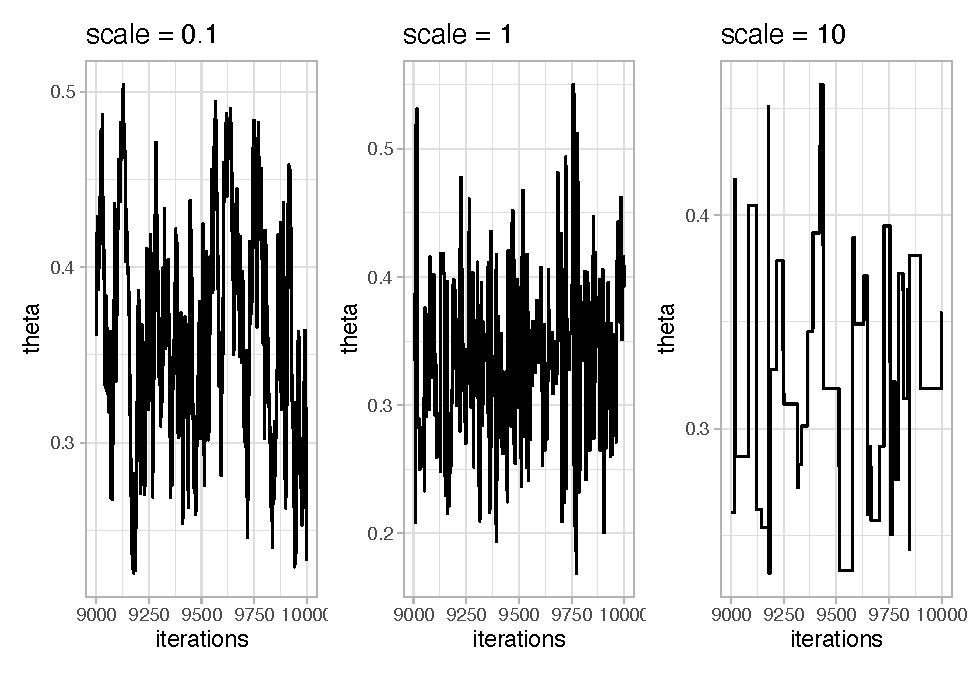
\includegraphics[width=1\linewidth]{banana-book_files/figure-latex/traceown-1} 

}

\caption{Trace plots for different values of the standard deviation (scale) of the proposal distribution.}\label{fig:traceown}
\end{figure}

\hypertarget{tips-and-tricks}{%
\section{Tips and tricks}\label{tips-and-tricks}}

Before closing this chapter on NIMBLE, I thought it'd be useful to have a section gathering a few tips and tricks that would make your life easier. \textbf{These are my tips and tricks, NIMBLE users, I'd be happy to hear yours: \href{mailto:olivier.gimenez@cefe.cnrs.fr}{email me}, \href{https://github.com/oliviergimenez/banana-book/edit/master/nimble.Rmd}{edit the chapter} or \href{https://github.com/oliviergimenez/banana-book/issues}{file an issue} on GitHub.}

\hypertarget{precision-vs-standard-deviation}{%
\subsection{Precision vs standard deviation}\label{precision-vs-standard-deviation}}

In other sotware like JAGS, the normal distribution is parameterized with mean \texttt{mu} and a parameter called precision, often denoted \texttt{tau}, the inverse of the variance you are used to. Say we use a normal prior on some parameter \texttt{epsilon} with \texttt{epsilon\ \textasciitilde{}\ dnorm(mu,\ tau)}. We'd like this prior to be vague, therefore \texttt{tau} should be small, say 0.01 so that the variance of the normal distribution is large, 1/0.01 = 100 here. This subtlety is the source of problems (and frustration) when you forget that the second parameter is precision and use \texttt{epsilon\ \textasciitilde{}\ dnorm(mu,\ 100)}, because then the variance is actually 1/100 = 0.01 and the prior is very informative, and peaked on \texttt{mu}. In NIMBLE you can use this parameterisation as well as the more natural parameterisation \texttt{epsilon\ \textasciitilde{}\ dnorm(mu,\ sd\ =\ 100)} which avoids confusion.

\hypertarget{indexing}{%
\subsection{Indexing}\label{indexing}}

NIMBLE does not guess the dimensions of objects. In other software like JAGS you can write \texttt{sum.x\ \textless{}-\ sum(x{[}{]})} to calculate the sum over all components of \texttt{x}. In NIMBLE you need to write \texttt{sum.x\ \textless{}-\ sum(x{[}1:n{]})} to sum the components of \texttt{x} from 1 up to n.~Specifying dimensions can be annoying, but I find it useful as it forces me to think of what I am doing and to keep my code self-explaining.

\hypertarget{faster-compilation}{%
\subsection{Faster compilation}\label{faster-compilation}}

You might have noticed that compilation in NIMBLE takes time. When you have large models (with lots of nodes), compilation can take forever. You can set \texttt{calculate\ =\ FALSE} in \texttt{nimbleModel()} to disable the calculation of all deterministic nodes and log-likelihood. You can also use \texttt{useConjugacy\ =\ FALSE} in \texttt{configureMCMC()} to disable the search for conjugate samplers. With the animal survival example, you would do:

\begin{Shaded}
\begin{Highlighting}[]
\NormalTok{model }\OtherTok{\textless{}{-}} \FunctionTok{nimbleCode}\NormalTok{(\{}
  \CommentTok{\# likelihood}
\NormalTok{  survived }\SpecialCharTok{\textasciitilde{}} \FunctionTok{dbinom}\NormalTok{(theta, released)}
  \CommentTok{\# prior}
\NormalTok{  theta }\SpecialCharTok{\textasciitilde{}} \FunctionTok{dunif}\NormalTok{(}\DecValTok{0}\NormalTok{, }\DecValTok{1}\NormalTok{)}
\NormalTok{\})}
\NormalTok{my.data }\OtherTok{\textless{}{-}} \FunctionTok{list}\NormalTok{(}\AttributeTok{survived =} \DecValTok{19}\NormalTok{, }\AttributeTok{released =} \DecValTok{57}\NormalTok{)}
\NormalTok{initial.values }\OtherTok{\textless{}{-}} \ControlFlowTok{function}\NormalTok{() }\FunctionTok{list}\NormalTok{(}\AttributeTok{theta =} \FunctionTok{runif}\NormalTok{(}\DecValTok{1}\NormalTok{,}\DecValTok{0}\NormalTok{,}\DecValTok{1}\NormalTok{))}
\NormalTok{survival }\OtherTok{\textless{}{-}} \FunctionTok{nimbleModel}\NormalTok{(}\AttributeTok{code =}\NormalTok{ model, }
                        \AttributeTok{data =}\NormalTok{ my.data, }
                        \AttributeTok{inits =} \FunctionTok{initial.values}\NormalTok{(),}
                        \AttributeTok{calculate =} \ConstantTok{FALSE}\NormalTok{) }\CommentTok{\# first tip}
\NormalTok{Csurvival }\OtherTok{\textless{}{-}} \FunctionTok{compileNimble}\NormalTok{(survival)}
\NormalTok{survivalConf }\OtherTok{\textless{}{-}} \FunctionTok{configureMCMC}\NormalTok{(survival)}
\DocumentationTok{\#\# ===== Monitors =====}
\DocumentationTok{\#\# thin = 1: theta}
\DocumentationTok{\#\# ===== Samplers =====}
\DocumentationTok{\#\# RW sampler (1)}
\DocumentationTok{\#\#   {-} theta}
\NormalTok{survivalMCMC }\OtherTok{\textless{}{-}} \FunctionTok{buildMCMC}\NormalTok{(survivalConf, }\AttributeTok{useConjugacy =} \ConstantTok{FALSE}\NormalTok{) }\CommentTok{\# second tip}
\NormalTok{CsurvivalMCMC }\OtherTok{\textless{}{-}} \FunctionTok{compileNimble}\NormalTok{(survivalMCMC, }
                               \AttributeTok{project =}\NormalTok{ survival)}
\NormalTok{samples }\OtherTok{\textless{}{-}} \FunctionTok{runMCMC}\NormalTok{(}\AttributeTok{mcmc =}\NormalTok{ CsurvivalMCMC, }
                   \AttributeTok{niter =} \DecValTok{5000}\NormalTok{, }
                   \AttributeTok{nburnin =} \DecValTok{1000}\NormalTok{)}
\DocumentationTok{\#\# |{-}{-}{-}{-}{-}{-}{-}{-}{-}{-}{-}{-}{-}|{-}{-}{-}{-}{-}{-}{-}{-}{-}{-}{-}{-}{-}|{-}{-}{-}{-}{-}{-}{-}{-}{-}{-}{-}{-}{-}|{-}{-}{-}{-}{-}{-}{-}{-}{-}{-}{-}{-}{-}|}
\DocumentationTok{\#\# |{-}{-}{-}{-}{-}{-}{-}{-}{-}{-}{-}{-}{-}{-}{-}{-}{-}{-}{-}{-}{-}{-}{-}{-}{-}{-}{-}{-}{-}{-}{-}{-}{-}{-}{-}{-}{-}{-}{-}{-}{-}{-}{-}{-}{-}{-}{-}{-}{-}{-}{-}{-}{-}{-}{-}|}
\FunctionTok{samplesSummary}\NormalTok{(samples)}
\DocumentationTok{\#\#         Mean Median St.Dev. 95\%CI\_low 95\%CI\_upp}
\DocumentationTok{\#\# theta 0.3402 0.3391 0.06029    0.2258    0.4616}
\end{Highlighting}
\end{Shaded}

\hypertarget{updating-mcmc-chains}{%
\subsection{Updating MCMC chains}\label{updating-mcmc-chains}}

Sometimes it is useful to run your MCMC chains a little bit longer to improve convergence. Re-starting from the run in previous section, you can use:

\begin{Shaded}
\begin{Highlighting}[]
\NormalTok{niter\_ad }\OtherTok{\textless{}{-}} \DecValTok{6000}
\NormalTok{CsurvivalMCMC}\SpecialCharTok{$}\FunctionTok{run}\NormalTok{(niter\_ad, }\AttributeTok{reset =} \ConstantTok{FALSE}\NormalTok{)}
\DocumentationTok{\#\# |{-}{-}{-}{-}{-}{-}{-}{-}{-}{-}{-}{-}{-}|{-}{-}{-}{-}{-}{-}{-}{-}{-}{-}{-}{-}{-}|{-}{-}{-}{-}{-}{-}{-}{-}{-}{-}{-}{-}{-}|{-}{-}{-}{-}{-}{-}{-}{-}{-}{-}{-}{-}{-}|}
\DocumentationTok{\#\# |{-}{-}{-}{-}{-}{-}{-}{-}{-}{-}{-}{-}{-}{-}{-}{-}{-}{-}{-}{-}{-}{-}{-}{-}{-}{-}{-}{-}{-}{-}{-}{-}{-}{-}{-}{-}{-}{-}{-}{-}{-}{-}{-}{-}{-}{-}{-}{-}{-}{-}{-}{-}{-}{-}{-}|}
\DocumentationTok{\#\# NULL}
\end{Highlighting}
\end{Shaded}

Then you can extract the matrix of previous MCMC samples augmented with new ones and obtain numerical summaries:

\begin{Shaded}
\begin{Highlighting}[]
\NormalTok{more\_samples }\OtherTok{\textless{}{-}} \FunctionTok{as.matrix}\NormalTok{(CsurvivalMCMC}\SpecialCharTok{$}\NormalTok{mvSamples)}
\FunctionTok{samplesSummary}\NormalTok{(more\_samples)}
\DocumentationTok{\#\#         Mean Median St.Dev. 95\%CI\_low 95\%CI\_upp}
\DocumentationTok{\#\# theta 0.3402 0.3382 0.05975    0.2281    0.4632}
\end{Highlighting}
\end{Shaded}

You can check that \texttt{more\_samples} contains 10000 samples, 4000 from the call to \texttt{runMCMC()} plus 6000 additional samples.

\hypertarget{reproducibility}{%
\subsection{Reproducibility}\label{reproducibility}}

If you want your results to be reproducible, you can control the state of R the random number generator with the \texttt{setSeed} argument in functions \texttt{nimbleMCMC()} and \texttt{runMCMC()}. Going back to the animal survival example, you can check that two calls to \texttt{nimbleMCMC()} give the same results when \texttt{setSeed} is set to the same value:

\begin{Shaded}
\begin{Highlighting}[]
\CommentTok{\# first call to nimbleMCMC()}
\NormalTok{mcmc.output1 }\OtherTok{\textless{}{-}} \FunctionTok{nimbleMCMC}\NormalTok{(}\AttributeTok{code =}\NormalTok{ model,}
                           \AttributeTok{data =}\NormalTok{ my.data,}
                           \AttributeTok{inits =}\NormalTok{ initial.values,}
                           \AttributeTok{niter =} \DecValTok{5000}\NormalTok{,}
                           \AttributeTok{nburnin =} \DecValTok{1000}\NormalTok{,}
                           \AttributeTok{nchains =} \DecValTok{3}\NormalTok{,}
                           \AttributeTok{summary =} \ConstantTok{TRUE}\NormalTok{,}
                           \AttributeTok{setSeed =} \DecValTok{123}\NormalTok{)}
\DocumentationTok{\#\# |{-}{-}{-}{-}{-}{-}{-}{-}{-}{-}{-}{-}{-}|{-}{-}{-}{-}{-}{-}{-}{-}{-}{-}{-}{-}{-}|{-}{-}{-}{-}{-}{-}{-}{-}{-}{-}{-}{-}{-}|{-}{-}{-}{-}{-}{-}{-}{-}{-}{-}{-}{-}{-}|}
\DocumentationTok{\#\# |{-}{-}{-}{-}{-}{-}{-}{-}{-}{-}{-}{-}{-}{-}{-}{-}{-}{-}{-}{-}{-}{-}{-}{-}{-}{-}{-}{-}{-}{-}{-}{-}{-}{-}{-}{-}{-}{-}{-}{-}{-}{-}{-}{-}{-}{-}{-}{-}{-}{-}{-}{-}{-}{-}{-}|}
\DocumentationTok{\#\# |{-}{-}{-}{-}{-}{-}{-}{-}{-}{-}{-}{-}{-}|{-}{-}{-}{-}{-}{-}{-}{-}{-}{-}{-}{-}{-}|{-}{-}{-}{-}{-}{-}{-}{-}{-}{-}{-}{-}{-}|{-}{-}{-}{-}{-}{-}{-}{-}{-}{-}{-}{-}{-}|}
\DocumentationTok{\#\# |{-}{-}{-}{-}{-}{-}{-}{-}{-}{-}{-}{-}{-}{-}{-}{-}{-}{-}{-}{-}{-}{-}{-}{-}{-}{-}{-}{-}{-}{-}{-}{-}{-}{-}{-}{-}{-}{-}{-}{-}{-}{-}{-}{-}{-}{-}{-}{-}{-}{-}{-}{-}{-}{-}{-}|}
\DocumentationTok{\#\# |{-}{-}{-}{-}{-}{-}{-}{-}{-}{-}{-}{-}{-}|{-}{-}{-}{-}{-}{-}{-}{-}{-}{-}{-}{-}{-}|{-}{-}{-}{-}{-}{-}{-}{-}{-}{-}{-}{-}{-}|{-}{-}{-}{-}{-}{-}{-}{-}{-}{-}{-}{-}{-}|}
\DocumentationTok{\#\# |{-}{-}{-}{-}{-}{-}{-}{-}{-}{-}{-}{-}{-}{-}{-}{-}{-}{-}{-}{-}{-}{-}{-}{-}{-}{-}{-}{-}{-}{-}{-}{-}{-}{-}{-}{-}{-}{-}{-}{-}{-}{-}{-}{-}{-}{-}{-}{-}{-}{-}{-}{-}{-}{-}{-}|}
\CommentTok{\# second call to nimbleMCMC()}
\NormalTok{mcmc.output2 }\OtherTok{\textless{}{-}} \FunctionTok{nimbleMCMC}\NormalTok{(}\AttributeTok{code =}\NormalTok{ model,}
                           \AttributeTok{data =}\NormalTok{ my.data,}
                           \AttributeTok{inits =}\NormalTok{ initial.values,}
                           \AttributeTok{niter =} \DecValTok{5000}\NormalTok{,}
                           \AttributeTok{nburnin =} \DecValTok{1000}\NormalTok{,}
                           \AttributeTok{nchains =} \DecValTok{3}\NormalTok{,}
                           \AttributeTok{summary =} \ConstantTok{TRUE}\NormalTok{,}
                           \AttributeTok{setSeed =} \DecValTok{123}\NormalTok{)}
\DocumentationTok{\#\# |{-}{-}{-}{-}{-}{-}{-}{-}{-}{-}{-}{-}{-}|{-}{-}{-}{-}{-}{-}{-}{-}{-}{-}{-}{-}{-}|{-}{-}{-}{-}{-}{-}{-}{-}{-}{-}{-}{-}{-}|{-}{-}{-}{-}{-}{-}{-}{-}{-}{-}{-}{-}{-}|}
\DocumentationTok{\#\# |{-}{-}{-}{-}{-}{-}{-}{-}{-}{-}{-}{-}{-}{-}{-}{-}{-}{-}{-}{-}{-}{-}{-}{-}{-}{-}{-}{-}{-}{-}{-}{-}{-}{-}{-}{-}{-}{-}{-}{-}{-}{-}{-}{-}{-}{-}{-}{-}{-}{-}{-}{-}{-}{-}{-}|}
\DocumentationTok{\#\# |{-}{-}{-}{-}{-}{-}{-}{-}{-}{-}{-}{-}{-}|{-}{-}{-}{-}{-}{-}{-}{-}{-}{-}{-}{-}{-}|{-}{-}{-}{-}{-}{-}{-}{-}{-}{-}{-}{-}{-}|{-}{-}{-}{-}{-}{-}{-}{-}{-}{-}{-}{-}{-}|}
\DocumentationTok{\#\# |{-}{-}{-}{-}{-}{-}{-}{-}{-}{-}{-}{-}{-}{-}{-}{-}{-}{-}{-}{-}{-}{-}{-}{-}{-}{-}{-}{-}{-}{-}{-}{-}{-}{-}{-}{-}{-}{-}{-}{-}{-}{-}{-}{-}{-}{-}{-}{-}{-}{-}{-}{-}{-}{-}{-}|}
\DocumentationTok{\#\# |{-}{-}{-}{-}{-}{-}{-}{-}{-}{-}{-}{-}{-}|{-}{-}{-}{-}{-}{-}{-}{-}{-}{-}{-}{-}{-}|{-}{-}{-}{-}{-}{-}{-}{-}{-}{-}{-}{-}{-}|{-}{-}{-}{-}{-}{-}{-}{-}{-}{-}{-}{-}{-}|}
\DocumentationTok{\#\# |{-}{-}{-}{-}{-}{-}{-}{-}{-}{-}{-}{-}{-}{-}{-}{-}{-}{-}{-}{-}{-}{-}{-}{-}{-}{-}{-}{-}{-}{-}{-}{-}{-}{-}{-}{-}{-}{-}{-}{-}{-}{-}{-}{-}{-}{-}{-}{-}{-}{-}{-}{-}{-}{-}{-}|}
\CommentTok{\# outputs from both calls are the same}
\NormalTok{mcmc.output1}\SpecialCharTok{$}\NormalTok{summary}\SpecialCharTok{$}\NormalTok{all.chains}
\DocumentationTok{\#\#         Mean Median St.Dev. 95\%CI\_low 95\%CI\_upp}
\DocumentationTok{\#\# theta 0.3387  0.336 0.05968    0.2282    0.4608}
\NormalTok{mcmc.output2}\SpecialCharTok{$}\NormalTok{summary}\SpecialCharTok{$}\NormalTok{all.chains}
\DocumentationTok{\#\#         Mean Median St.Dev. 95\%CI\_low 95\%CI\_upp}
\DocumentationTok{\#\# theta 0.3387  0.336 0.05968    0.2282    0.4608}
\end{Highlighting}
\end{Shaded}

\hypertarget{parallelization}{%
\subsection{Parallelization}\label{parallelization}}

To speed up your analyses, you can run MCMC chains in parallel. This is what the package \texttt{jagsUI}\footnote{\url{https://github.com/kenkellner/jagsUI}} accomplishes for JAGS users. Here, we use the \texttt{parallel} package for parallel computation:

\begin{Shaded}
\begin{Highlighting}[]
\FunctionTok{library}\NormalTok{(parallel)}
\end{Highlighting}
\end{Shaded}

First you create a cluster using the total amount of cores you have but one to make sure your computer can go on working:

\begin{Shaded}
\begin{Highlighting}[]
\NormalTok{nbcores }\OtherTok{\textless{}{-}} \FunctionTok{detectCores}\NormalTok{() }\SpecialCharTok{{-}} \DecValTok{1}
\NormalTok{my\_cluster }\OtherTok{\textless{}{-}} \FunctionTok{makeCluster}\NormalTok{(nbcores)}
\end{Highlighting}
\end{Shaded}

Then you wrap your workflow in a function to be run in parallel:

\begin{Shaded}
\begin{Highlighting}[]
\NormalTok{workflow }\OtherTok{\textless{}{-}} \ControlFlowTok{function}\NormalTok{(seed, data) \{}
  
  \FunctionTok{library}\NormalTok{(nimble)}
  
\NormalTok{  model }\OtherTok{\textless{}{-}} \FunctionTok{nimbleCode}\NormalTok{(\{}
    \CommentTok{\# likelihood}
\NormalTok{    survived }\SpecialCharTok{\textasciitilde{}} \FunctionTok{dbinom}\NormalTok{(theta, released)}
    \CommentTok{\# prior}
\NormalTok{    theta }\SpecialCharTok{\textasciitilde{}} \FunctionTok{dunif}\NormalTok{(}\DecValTok{0}\NormalTok{, }\DecValTok{1}\NormalTok{)}
\NormalTok{  \})}
  
  \FunctionTok{set.seed}\NormalTok{(}\DecValTok{123}\NormalTok{) }\CommentTok{\# for reproducibility}
\NormalTok{  initial.values }\OtherTok{\textless{}{-}} \ControlFlowTok{function}\NormalTok{() }\FunctionTok{list}\NormalTok{(}\AttributeTok{theta =} \FunctionTok{runif}\NormalTok{(}\DecValTok{1}\NormalTok{,}\DecValTok{0}\NormalTok{,}\DecValTok{1}\NormalTok{))}
  
\NormalTok{  survival }\OtherTok{\textless{}{-}} \FunctionTok{nimbleModel}\NormalTok{(}\AttributeTok{code =}\NormalTok{ model, }
                          \AttributeTok{data =}\NormalTok{ data, }
                          \AttributeTok{inits =} \FunctionTok{initial.values}\NormalTok{())}
\NormalTok{  Csurvival }\OtherTok{\textless{}{-}} \FunctionTok{compileNimble}\NormalTok{(survival)}
\NormalTok{  survivalMCMC }\OtherTok{\textless{}{-}} \FunctionTok{buildMCMC}\NormalTok{(Csurvival)}
\NormalTok{  CsurvivalMCMC }\OtherTok{\textless{}{-}} \FunctionTok{compileNimble}\NormalTok{(survivalMCMC)}
  
\NormalTok{  samples }\OtherTok{\textless{}{-}} \FunctionTok{runMCMC}\NormalTok{(}\AttributeTok{mcmc =}\NormalTok{ CsurvivalMCMC, }
                     \AttributeTok{niter =} \DecValTok{5000}\NormalTok{, }
                     \AttributeTok{nburnin =} \DecValTok{1000}\NormalTok{,}
                     \AttributeTok{setSeed =}\NormalTok{ seed)}
  
  \FunctionTok{return}\NormalTok{(samples)}
\NormalTok{\}}
\end{Highlighting}
\end{Shaded}

Now we run the code using \texttt{parLapply()}, which uses cluster nodes to execute our workflow:

\begin{Shaded}
\begin{Highlighting}[]
\NormalTok{output }\OtherTok{\textless{}{-}} \FunctionTok{parLapply}\NormalTok{(}\AttributeTok{cl =}\NormalTok{ my\_cluster, }
                    \AttributeTok{X =} \FunctionTok{c}\NormalTok{(}\DecValTok{2022}\NormalTok{, }\DecValTok{666}\NormalTok{),}
                    \AttributeTok{fun =}\NormalTok{ workflow, }
                    \AttributeTok{data =} \FunctionTok{list}\NormalTok{(}\AttributeTok{survived =} \DecValTok{19}\NormalTok{, }\AttributeTok{released =} \DecValTok{57}\NormalTok{))}
\end{Highlighting}
\end{Shaded}

In the call to \texttt{parLapply}, we specify \texttt{X\ =\ c(2022,\ 666)} to ensure reproducibility. We use two alues 2022 and 666 to set the seed in \texttt{workflow()}, which means we run two instances of our workflow, or two MCMC chains. Note that we also have a line \texttt{set.seed(123)} in the \texttt{workflow()} function to ensure reproducibility while drawing randomly initial values.

It's good practice to close the cluster with \texttt{stopCluster()} so that processes do not continue to run in the background and slow down other processes:

\begin{Shaded}
\begin{Highlighting}[]
\FunctionTok{stopCluster}\NormalTok{(my\_cluster)}
\end{Highlighting}
\end{Shaded}

By inspecting the results, you can see that the object \texttt{output} is a list with two components, one for each MCMC chain:

\begin{Shaded}
\begin{Highlighting}[]
\FunctionTok{str}\NormalTok{(output)}
\DocumentationTok{\#\# List of 2}
\DocumentationTok{\#\#  $ : num [1:4000, 1] 0.393 0.369 0.346 0.346 0.346 ...}
\DocumentationTok{\#\#   ..{-} attr(*, "dimnames")=List of 2}
\DocumentationTok{\#\#   .. ..$ : NULL}
\DocumentationTok{\#\#   .. ..$ : chr "theta"}
\DocumentationTok{\#\#  $ : num [1:4000, 1] 0.435 0.435 0.435 0.435 0.243 ...}
\DocumentationTok{\#\#   ..{-} attr(*, "dimnames")=List of 2}
\DocumentationTok{\#\#   .. ..$ : NULL}
\DocumentationTok{\#\#   .. ..$ : chr "theta"}
\end{Highlighting}
\end{Shaded}

Eventually, you can obtain numerical summaries:

\begin{Shaded}
\begin{Highlighting}[]
\FunctionTok{MCMCsummary}\NormalTok{(output)}
\DocumentationTok{\#\#         mean      sd   2.5\%    50\%  97.5\% Rhat n.eff}
\DocumentationTok{\#\# theta 0.3361 0.06148 0.2215 0.3335 0.4594    1  1779}
\end{Highlighting}
\end{Shaded}

\hypertarget{incomplete-initialization}{%
\subsection{Incomplete initialization}\label{incomplete-initialization}}

When you run \texttt{nimbleMCMC()} or \texttt{nimbleModel()}, you may get warnings thrown at you by NIMBLE like `This model is not fully initialized' or `value is NA or NaN even after trying to calculate'. This is not necessarily an error, but it `reflects missing values in model variables' (incomplete initialization). In this situation, NIMBLE will initialize nodes with NAs by drawing from priors, and it will work or not. When possible, I try to initialize all nodes (full initialization). The process can be a bit of a headache, but it helps understanding the model structure better. Going back to our animal survival example, let's purposedly forget to provide an initial value for \texttt{theta}:

\begin{Shaded}
\begin{Highlighting}[]
\NormalTok{model }\OtherTok{\textless{}{-}} \FunctionTok{nimbleCode}\NormalTok{(\{}
  \CommentTok{\# likelihood}
\NormalTok{  survived }\SpecialCharTok{\textasciitilde{}} \FunctionTok{dbinom}\NormalTok{(theta, released)}
  \CommentTok{\# prior}
\NormalTok{  theta }\SpecialCharTok{\textasciitilde{}} \FunctionTok{dunif}\NormalTok{(}\DecValTok{0}\NormalTok{, }\DecValTok{1}\NormalTok{)}
\NormalTok{\})}
\CommentTok{\#initial.values \textless{}{-} list(theta = runif(1,0,1))}
\NormalTok{survival }\OtherTok{\textless{}{-}} \FunctionTok{nimbleModel}\NormalTok{(}\AttributeTok{code =}\NormalTok{ model, }
                        \AttributeTok{data =} \FunctionTok{list}\NormalTok{(}\AttributeTok{survived =} \DecValTok{19}\NormalTok{, }\AttributeTok{released =} \DecValTok{57}\NormalTok{))}
\end{Highlighting}
\end{Shaded}

To see which variables are not initialized, we use \texttt{initializeInfo()}:

\begin{Shaded}
\begin{Highlighting}[]
\CommentTok{\# survival$calculate() \# gives NA}
\NormalTok{survival}\SpecialCharTok{$}\FunctionTok{initializeInfo}\NormalTok{()}
\end{Highlighting}
\end{Shaded}

Now that we know \texttt{theta} was not initialized, we can fix the issue and resume our workflow:

\begin{Shaded}
\begin{Highlighting}[]
\NormalTok{survival}\SpecialCharTok{$}\NormalTok{theta }\OtherTok{\textless{}{-}} \FloatTok{0.5} \CommentTok{\# assign initial value to theta}
\NormalTok{survival}\SpecialCharTok{$}\FunctionTok{calculate}\NormalTok{() }
\DocumentationTok{\#\# [1] {-}5.422}

\NormalTok{Csurvival }\OtherTok{\textless{}{-}} \FunctionTok{compileNimble}\NormalTok{(survival)}
\NormalTok{survivalMCMC }\OtherTok{\textless{}{-}} \FunctionTok{buildMCMC}\NormalTok{(Csurvival)}
\DocumentationTok{\#\# ===== Monitors =====}
\DocumentationTok{\#\# thin = 1: theta}
\DocumentationTok{\#\# ===== Samplers =====}
\DocumentationTok{\#\# RW sampler (1)}
\DocumentationTok{\#\#   {-} theta}
\NormalTok{CsurvivalMCMC }\OtherTok{\textless{}{-}} \FunctionTok{compileNimble}\NormalTok{(survivalMCMC)}

\NormalTok{samples }\OtherTok{\textless{}{-}} \FunctionTok{runMCMC}\NormalTok{(}\AttributeTok{mcmc =}\NormalTok{ CsurvivalMCMC, }
                   \AttributeTok{niter =} \DecValTok{5000}\NormalTok{, }
                   \AttributeTok{nburnin =} \DecValTok{1000}\NormalTok{)}
\DocumentationTok{\#\# |{-}{-}{-}{-}{-}{-}{-}{-}{-}{-}{-}{-}{-}|{-}{-}{-}{-}{-}{-}{-}{-}{-}{-}{-}{-}{-}|{-}{-}{-}{-}{-}{-}{-}{-}{-}{-}{-}{-}{-}|{-}{-}{-}{-}{-}{-}{-}{-}{-}{-}{-}{-}{-}|}
\DocumentationTok{\#\# |{-}{-}{-}{-}{-}{-}{-}{-}{-}{-}{-}{-}{-}{-}{-}{-}{-}{-}{-}{-}{-}{-}{-}{-}{-}{-}{-}{-}{-}{-}{-}{-}{-}{-}{-}{-}{-}{-}{-}{-}{-}{-}{-}{-}{-}{-}{-}{-}{-}{-}{-}{-}{-}{-}{-}|}

\FunctionTok{samplesSummary}\NormalTok{(samples)}
\DocumentationTok{\#\#         Mean Median St.Dev. 95\%CI\_low 95\%CI\_upp}
\DocumentationTok{\#\# theta 0.3359 0.3335 0.06088    0.2191    0.4602}
\end{Highlighting}
\end{Shaded}

\hypertarget{vectorization}{%
\subsection{Vectorization}\label{vectorization}}

Vectorization is the process of replacing a loop by a vector so that instead of processing a single value at a time, you process a set of values at once. As an example, instead of writing:

\begin{Shaded}
\begin{Highlighting}[]
\ControlFlowTok{for}\NormalTok{(i }\ControlFlowTok{in} \DecValTok{1}\SpecialCharTok{:}\NormalTok{n)\{ }
\NormalTok{  x[i] }\OtherTok{\textless{}{-}}\NormalTok{ mu }\SpecialCharTok{+}\NormalTok{ epsilon[i] }
\NormalTok{\}}
\end{Highlighting}
\end{Shaded}

you would write:

\begin{Shaded}
\begin{Highlighting}[]
\NormalTok{x[}\DecValTok{1}\SpecialCharTok{:}\NormalTok{n] }\OtherTok{\textless{}{-}}\NormalTok{ mu }\SpecialCharTok{+}\NormalTok{ epsilon[}\DecValTok{1}\SpecialCharTok{:}\NormalTok{n]}
\end{Highlighting}
\end{Shaded}

Vectorization can make your code more efficient by manipulating one vector node \texttt{x{[}1:n{]}} instead of \texttt{n} nodes \texttt{x{[}1{]}}, \ldots, \texttt{x{[}n{]}}. \textbf{Think of an example in relation to animal survival? Illustrate with vectorized Bernoulli or \href{https://github.com/nimble-dev/nimbleSCR/blob/master/nimbleSCR/R/dbinom_vector.R}{vectorized Binomial}?}

\hypertarget{summary-1}{%
\section{Summary}\label{summary-1}}

\begin{itemize}
\item
  NIMBLE is an R package that implements for you MCMC algorithms to generate samples from the posterior distribution of model parameters. You only have to specify a likelihood and priors using the BUGS language to apply the Bayes theorem.
\item
  NIMBLE is more than just another MCMC engine. It provides a programming environment so that you have full control when building models and estimating parameters.
\item
  At the core of NIMBLE are \texttt{nimbleFunctions} which you can write and compile for faster computation. With \texttt{nimbleFunctions} you can mimic basic R syntax, work with vectors and matrices, use logical operators and flow control, and specify many distributions.
\item
  There are two workflows to run NIMBLE. In most situations, \texttt{nimbleMCMC()} will serve you well. When you need more control, you can adopt a detailed workflow with \texttt{nimbleModel()}, \texttt{configureMCMC()}, \texttt{buildMCMC()}, \texttt{compileNimble()} and \texttt{runMCMC()}.
\item
  By having full control of the workflow, you can change default MCMC samplers and even write your own samplers.
\end{itemize}

\hypertarget{suggested-reading-1}{%
\section{Suggested reading}\label{suggested-reading-1}}

In this chapter, I have only scratched the surface of what NIMBLE is capable of. Below is a list of pointers that should help you going further with NIMBLE.

\begin{itemize}
\item
  The NIMBLE folks make a lot of useful resources available through the official website \url{https://r-nimble.org}.
\item
  The NIMBLE manual \url{https://r-nimble.org/html_manual/cha-welcome-nimble.html} reads like a book with clear explanations and relevant examples.
\item
  You can learn a lot by going through examples at \url{https://r-nimble.org/examples} and training material from NIMBLE workshops at \url{https://github.com/nimble-training}.
\item
  You can keep the NIMBLE cheatsheet \url{https://r-nimble.org/cheatsheets/NimbleCheatSheet.pdf} near you to remind yourself of the workflow, how to write and use models, or which functions and distributions are available.
\item
  The motivation to write this book comes from a workshop I co-teach with colleagues, including Perry de Valpine and Daniel Turek from the NIMBLE development team. The material (slides and videos) is available at \url{https://github.com/oliviergimenez/bayesian-cr-workshop}.
\item
  If you have questions, feel free to get in touch with the community of NIMBLE users by emailing the discussion group \url{https://groups.google.com/forum/\#!forum/nimble-users}. This is a great place to learn, and folks who take the time to answer questions are kind and provide constructive answers. When possible, make sure to provide a reproducible example illustrating your problem.
\item
  Last, you can cite the following reference when using NIMBLE in a publication:
\end{itemize}

\begin{quote}
de Valpine, P., D. Turek, C. J. Paciorek, C. Anderson-Bergman, D. Temple Lang, and R. Bodik (2017). \href{https://arxiv.org/pdf/1505.05093.pdf}{Programming With Models: Writing Statistical Algorithms for General Model Structures With NIMBLE}. \emph{Journal of Computational and Graphical Statistics} \textbf{26} (2): 403--13.
\end{quote}

\hypertarget{hmmcapturerecapture}{%
\chapter{Hidden Markov models}\label{hmmcapturerecapture}}

\hypertarget{introduction-3}{%
\section{Introduction}\label{introduction-3}}

In this third chapter, you will learn the basics on Markov models and how to fit them to longitudinal data using NIMBLE. In real life however, individuals may go undetected and their status be unknown. You will also learn how to manipulate the extension of Markov models to hidden states, so-called hidden Markov models.

\hypertarget{longitudinal-data}{%
\section{Longitudinal data}\label{longitudinal-data}}

Let's get back to our survival example, and denote \(z_i\) the state of individual \(i\) with \(z_i = 1\) if alive and \(z_i = 0\) if dead. We have a total of \(z = \displaystyle{\sum_{i=1}^{n}{z_i}}\) survivors out of \(n\) released animals with winter survival probability \(\phi\). Our model so far is a combination of a binomial likelihood and a Beta prior with parameters 1 and 1, which is also a uniform distribution between 0 and 1. It can be written as\footnote{I write models the way Richard McElreath does it in his book and video lectures \href{https://xcelab.net/rm/statistical-rethinking/}{Statistical Rethinking}.}:

\begin{align*}
   z &\sim \text{Binomial}(n, \phi) &\text{[likelihood]}
   \\
  \phi &\sim \text{Beta}(1, 1) &\text{[prior for }\phi \text{]} \\
\end{align*}

Because the binomial distribution is just a sum of independent Bernoulli outcomes, you can rewrite this model as:

\begin{align*}
   z_i &\sim \text{Bernoulli}(\phi), \; i = 1, \ldots, N &\text{[likelihood]}
   \\
  \phi &\sim \text{Beta}(1, 1) &\text{[prior for }\phi \text{]} \\
\end{align*}

It is like flipping a coin for each individual and get a survivor with probability \(\phi\).

In this set up, we consider a single winter. But for many species, we need to collect data on the long term to get a representative estimate of survival. Therefore what if we had say \(T = 5\) winters?

Let us denote \(z_{i,t} = 1\) if individual \(i\) alive at winter \(t\), and \(z_{i,t} = 2\) if dead. Then longitudinal data look like in the table below. Each row is an individual \(i\), and columns are for winters \(t\), or sampling occasions. Variable \(z\) is indexed by both \(i\) and \(t\), and takes value 1 if individual \(i\) is alive in winter \(t\), and 2 otherwise.

\begin{tabular}{r|r|r|r|r|r}
\hline
id & winter 1 & winter 2 & winter 3 & winter 4 & winter 5\\
\hline
1 & 1 & 1 & 1 & 1 & 1\\
\hline
2 & 1 & 1 & 1 & 1 & 1\\
\hline
3 & 1 & 1 & 1 & 1 & 1\\
\hline
4 & 1 & 1 & 1 & 1 & 2\\
\hline
5 & 1 & 1 & 1 & 1 & 1\\
\hline
6 & 1 & 1 & 2 & 2 & 2\\
\hline
7 & 1 & 1 & 1 & 1 & 1\\
\hline
8 & 1 & 2 & 2 & 2 & 2\\
\hline
9 & 1 & 1 & 1 & 1 & 2\\
\hline
10 & 1 & 2 & 2 & 2 & 2\\
\hline
11 & 1 & 1 & 1 & 1 & 1\\
\hline
12 & 1 & 1 & 1 & 1 & 1\\
\hline
13 & 1 & 1 & 1 & 2 & 2\\
\hline
14 & 1 & 1 & 1 & 1 & 1\\
\hline
15 & 1 & 2 & 2 & 2 & 2\\
\hline
16 & 1 & 1 & 1 & 1 & 1\\
\hline
17 & 1 & 1 & 1 & 1 & 1\\
\hline
18 & 1 & 1 & 1 & 1 & 2\\
\hline
19 & 1 & 1 & 1 & 1 & 1\\
\hline
20 & 1 & 1 & 2 & 2 & 2\\
\hline
21 & 1 & 1 & 2 & 2 & 2\\
\hline
22 & 1 & 2 & 2 & 2 & 2\\
\hline
23 & 1 & 1 & 1 & 1 & 2\\
\hline
24 & 1 & 1 & 1 & 1 & 2\\
\hline
25 & 1 & 1 & 1 & 1 & 1\\
\hline
26 & 1 & 1 & 1 & 1 & 2\\
\hline
27 & 1 & 1 & 1 & 1 & 2\\
\hline
28 & 1 & 2 & 2 & 2 & 2\\
\hline
29 & 1 & 1 & 2 & 2 & 2\\
\hline
30 & 1 & 1 & 2 & 2 & 2\\
\hline
31 & 1 & 2 & 2 & 2 & 2\\
\hline
32 & 1 & 2 & 2 & 2 & 2\\
\hline
33 & 1 & 2 & 2 & 2 & 2\\
\hline
34 & 1 & 1 & 2 & 2 & 2\\
\hline
35 & 1 & 1 & 2 & 2 & 2\\
\hline
36 & 1 & 2 & 2 & 2 & 2\\
\hline
37 & 1 & 1 & 1 & 1 & 1\\
\hline
38 & 1 & 1 & 1 & 2 & 2\\
\hline
39 & 1 & 1 & 1 & 1 & 1\\
\hline
40 & 1 & 1 & 1 & 1 & 2\\
\hline
41 & 1 & 1 & 1 & 1 & 1\\
\hline
42 & 1 & 1 & 1 & 2 & 2\\
\hline
43 & 1 & 1 & 1 & 1 & 1\\
\hline
44 & 1 & 1 & 2 & 2 & 2\\
\hline
45 & 1 & 1 & 1 & 2 & 2\\
\hline
46 & 1 & 1 & 1 & 1 & 1\\
\hline
47 & 1 & 1 & 1 & 1 & 1\\
\hline
48 & 1 & 2 & 2 & 2 & 2\\
\hline
49 & 1 & 1 & 1 & 1 & 1\\
\hline
50 & 1 & 1 & 1 & 2 & 2\\
\hline
51 & 1 & 1 & 1 & 1 & 2\\
\hline
52 & 1 & 1 & 1 & 2 & 2\\
\hline
53 & 1 & 1 & 1 & 1 & 1\\
\hline
54 & 1 & 1 & 1 & 1 & 1\\
\hline
55 & 1 & 2 & 2 & 2 & 2\\
\hline
56 & 1 & 1 & 1 & 1 & 1\\
\hline
57 & 1 & 1 & 1 & 2 & 2\\
\hline
\end{tabular}

\hypertarget{a-markov-model-for-longitudinal-data}{%
\section{A Markov model for longitudinal data}\label{a-markov-model-for-longitudinal-data}}

Let's think of a model for these data. The objective remains the same, estimating survival. To build this model, we'll make assumptions, go through its components and write down its likelihood. Note that we already encountered Markov models in Section \ref{markovmodelmcmc}.

\hypertarget{assumptions}{%
\subsection{Assumptions}\label{assumptions}}

First, we assume that the state of an animal in a given winter, alive or dead, is only dependent on its state the winter before. In other words, the future depends only on the present, not the past. This is a Markov process.

Second, if an animal is alive in a given winter, the probability it survives to the next winter is \(\phi\). The probability it dies is \(1 - \phi\).

Third, if an animal is dead a winter, it remains dead, unless you believe in zombies.

Our Markov process can be represented this way:

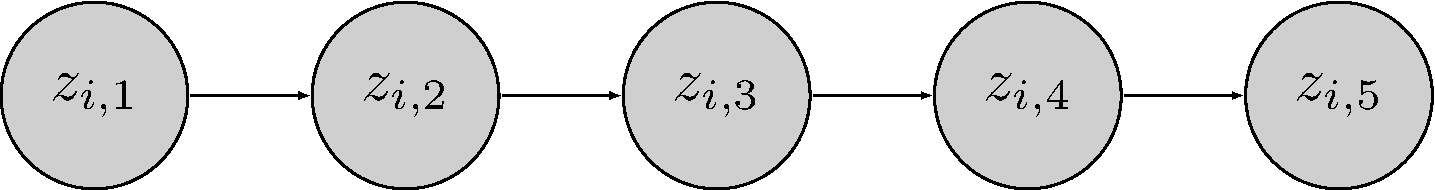
\includegraphics{banana-book_files/figure-latex/unnamed-chunk-110-1.pdf}

An example of this Markov process is, for example:

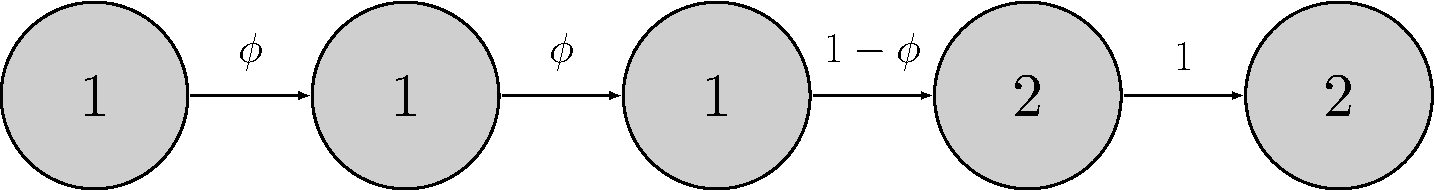
\includegraphics{banana-book_files/figure-latex/unnamed-chunk-111-1.pdf}

Here the animal remains alive over the first two time intervals \((z_{i,1} = z_{i,2} = z_{i,3} = 1)\) with probability \(\phi\) until it dies over the fourth time interval \((z_{i,4} = 2)\) with probability \(1-\phi\) then remains dead from then onwards \((z_{i,5} = 2)\) with probability 1.

\hypertarget{transition-matrix}{%
\subsection{Transition matrix}\label{transition-matrix}}

You might have figured it out already (if not, not a problem), the core of our Markov process is made of transition probabilities between states alive and dead. For example, the probability of transitioning from state alive at \(t-1\) to state alive at \(t\) is \(\Pr(z_{i,t} = 1 | z_{i,t-1} = 1) = \gamma_{1,1}\). It is the survival probability \(\phi\). The probability of dying over the interval \((t-1, t)\) is \(\Pr(z_{i,t} = 2 | z_{i,t-1} = 1) = \gamma_{1,2} = 1 - \phi\). Now if an animal is dead at \(t-1\), then \(\Pr(z_t = 1 | z_{t-1} = 2) = 0\) and \(\Pr(z_{i,t} = 2 | z_{i,t-1} = 2) = 1\).

We can gather these probabilities of transition between states from one occasion to the next in a matrix, say \(\mathbf{\Gamma}\), which we will call the transition matrix:

\begin{align*}
\mathbf{\Gamma} =
\left(\begin{array}{cc}
\gamma_{1,1} & \gamma_{1,2}\\
\gamma_{2,1} & \gamma_{2,2}
\end{array}\right) =
\left(\begin{array}{cc}
\phi & 1 - \phi\\
0 & 1
\end{array}\right)
\end{align*}

To try and remember that the states at \(t-1\) are in rows, and the states at \(t\) are in columns, I will often write:

\[
\begin{matrix}
& \\
\mathbf{\Gamma} =
    \left ( \vphantom{ \begin{matrix} 12 \\ 12 \end{matrix} } \right .
\end{matrix}
\hspace{-1.2em}
\begin{matrix}
    z_t=1 & z_t=2 \\ \hdashline
\phi & 1-\phi \\
0 & 1
\end{matrix}
\hspace{-0.2em}
\begin{matrix}
& \\
\left . \vphantom{ \begin{matrix} 12 \\ 12 \end{matrix} } \right )
    \begin{matrix}
    z_{t-1}=1 \; \mbox{(alive)} \\ z_{t-1}=2 \; \mbox{(dead)}
    \end{matrix}
\end{matrix}
\]

Take the time you need to navigate through this matrix, and get familiar with it. For example, you may start alive at \(t\) (first row) then end up dead at \(t+1\) (first column) with probability \(1-\phi\).

\hypertarget{initial-states}{%
\subsection{Initial states}\label{initial-states}}

A Markov process has to start somewhere. We need the probabilities of initial states, i.e.~the states of an individual at \(t = 1\). We will gather the probability of being in each state (alive or 1 and dead or 2) in the first winter in a vector. We will use \(\mathbf{\delta} = \left(\Pr(z_{i,1} = 1), \Pr(z_{i,1} = 2)\right)\). For simplicity, we will assume that all individuals are marked and released in the first winter, hence alive when first captured, which means that they are all in state alive or 1 for sure. Therefore we have \(\mathbf{\delta} = \left(1, 0\right)\).

\hypertarget{likelihood}{%
\subsection{Likelihood}\label{likelihood}}

Now that we have built a Markov model, we need its likelihood to apply the Bayes theorem. The likelihood is the probability of the data, given the model. Here the data are the \(z\), therefore we need \(\Pr(\mathbf{z}) = \Pr(z_1, z_2, \ldots, z_{T-2}, z_{T-1}, z_T)\).

We're gonna work backward, starting from the last sampling occasion. Using conditional probabilities, the likelihood can be written as the product of the probability of \(z_T\) i.e.~you're alive or not on the last occasion given your past history, that is the states at previous occasions, times the probability of your past history:

\begin{align*}
\Pr(\mathbf{z}) &= \Pr(z_T, z_{T-1}, z_{T-2}, \ldots, z_1) \color{white}{\Pr(z_{T-1}, z_{T-2},\ldots, z_1) \Pr(z_{T-2}, \ldots, z_1)}\\
                &= \color{blue}{\Pr(z_T | z_{T-1}, z_{T-2},\ldots, z_1) \Pr(z_{T-1}, z_{T-2},\ldots, z_1)} \\
\end{align*}

Then because we have a Markov model, we're memory less, that is the probabilty of next state, here \(z_T\), depends only on the current state, that is \(z_{T-1}\), and not the previous states:

\begin{align*}
\Pr(\mathbf{z}) &= \Pr(z_T, z_{T-1}, z_{T-2}, \ldots, z_1) \color{white}{\Pr(z_{T-1}, z_{T-2},\ldots, z_1) \Pr(z_{T-2}, \ldots, z_1)}\\
                &= \Pr(z_T | z_{T-1}, z_{T-2},\ldots, z_1) \Pr(z_{T-1}, z_{T-2},\ldots, z_1) \\
                &= \color{blue}{\Pr(z_T | z_{T-1})} \Pr(z_{T-1}, z_{T-2},\ldots, z_1) \\
\end{align*}

You can apply the same reasoning to \(T-1\). First use conditional probabilities:

\begin{align*}
\Pr(\mathbf{z}) &= \Pr(z_T, z_{T-1}, z_{T-2}, \ldots, z_1) \color{white}{\Pr(z_{T-1}, z_{T-2},\ldots, z_1) \Pr(z_{T-2}, \ldots, z_1)}\\
                &= \Pr(z_T | z_{T-1}, z_{T-2},\ldots, z_1) \Pr(z_{T-1}, z_{T-2},\ldots, z_1) \\
                &= \Pr(z_T | z_{T-1}) \Pr(z_{T-1}, z_{T-2},\ldots, z_1) \\
                &= \Pr(z_T | z_{T-1}) \color{blue}{\Pr(z_{T-1} | z_{T-2}, \ldots, z_1) \Pr(z_{T-2}, \ldots, z_1)}\\
\end{align*}

Then apply the Markovian property:

\begin{align*}
\Pr(\mathbf{z}) &= \Pr(z_T, z_{T-1}, z_{T-2}, \ldots, z_1) \color{white}{\Pr(z_{T-1}, z_{T-2},\ldots, z_1) \Pr(z_{T-2}, \ldots, z_1)}\\
                &= \Pr(z_T | z_{T-1}, z_{T-2},\ldots, z_1) \Pr(z_{T-1}, z_{T-2},\ldots, z_1) \\
                &= \Pr(z_T | z_{T-1}) \Pr(z_{T-1}, z_{T-2},\ldots, z_1) \\
                &= \Pr(z_T | z_{T-1}) \Pr(z_{T-1} | z_{T-2}, \ldots, z_1) \Pr(z_{T-2}, \ldots, z_1)\\
                &= \Pr(z_T | z_{T-1}) \color{blue}{\Pr(z_{T-1} | z_{T-2})} \Pr(z_{T-2}, \ldots, z_1)\\
\end{align*}

And so on up to \(z_2\). You end up with this expression for the likelihood:

\begin{align*}
\Pr(\mathbf{z}) &= \Pr(z_T, z_{T-1}, z_{T-2}, \ldots, z_1) \color{white}{\Pr(z_{T-1}, z_{T-2},\ldots, z_1) \Pr(z_{T-2}, \ldots, z_1)}\\
                &= \Pr(z_T | z_{T-1}, z_{T-2},\ldots, z_1) \Pr(z_{T-1}, z_{T-2},\ldots, z_1) \\
                &= \Pr(z_T | z_{T-1}) \Pr(z_{T-1}, z_{T-2},\ldots, z_1) \\
                &= \Pr(z_T | z_{T-1}) \Pr(z_{T-1} | z_{T-2}, \ldots, z_1) \Pr(z_{T-2}, \ldots, z_1)\\
                &= \Pr(z_T | z_{T-1}) \Pr(z_{T-1} | z_{T-2}) \Pr(z_{T-2}, \ldots, z_1)\\
                &= \ldots \\
                &= \color{blue}{\Pr(z_T | z_{T-1}) \Pr(z_{T-1} | z_{T-2}) \ldots \Pr(z_{2} | z_{1}) \Pr(z_{1})}\\
\end{align*}

This is a product of conditional probabilities of states given previous states, and the probability of initial states \(\Pr(z_1)\). Using a more compact notation for the product of conditional probabilities, we get:

\begin{align*}
\Pr(\mathbf{z}) &= \Pr(z_T, z_{T-1}, z_{T-2}, \ldots, z_1) \color{white}{\Pr(z_{T-1}, z_{T-2},\ldots, z_1) \Pr(z_{T-2}, \ldots, z_1)}\\
                &= \Pr(z_T | z_{T-1}, z_{T-2},\ldots, z_1) \Pr(z_{T-1}, z_{T-2},\ldots, z_1) \\
                &= \Pr(z_T | z_{T-1}) \Pr(z_{T-1}, z_{T-2},\ldots, z_1) \\
                &= \Pr(z_T | z_{T-1}) \Pr(z_{T-1} | z_{T-2}, \ldots, z_1) \Pr(z_{T-2}, \ldots, z_1)\\
                &= \Pr(z_T | z_{T-1}) \Pr(z_{T-1} | z_{T-2}) \Pr(z_{T-2}, \ldots, z_1)\\
                &= \ldots \\
                &= \Pr(z_T | z_{T-1}) \Pr(z_{T-1} | z_{T-2}) \ldots \Pr(z_{2} | z_{1}) \Pr(z_{1})\\
                &= \color{blue}{\Pr(z_{1}) \prod_{t=2}^T{\Pr(z_{t} | z_{t-1})}}\\
\end{align*}

In the product, you can recognize the transition parameters \(\gamma\) we defined above, so that the likelihood of a Markov model can be written as:

\begin{align*}
\Pr(\mathbf{z}) &= \Pr(z_T, z_{T-1}, z_{T-2}, \ldots, z_1) \color{white}{\Pr(z_{T-1}, z_{T-2},\ldots, z_1) \Pr(z_{T-2}, \ldots, z_1)}\\
                &= \Pr(z_{1}) \prod_{t=2}^T{\gamma_{z_{t-1},z_{t}}}\\
\end{align*}

\hypertarget{example}{%
\subsection{Example}\label{example}}

I realise these calculations are a bit difficult to follow. Let's take an example to fix ideas. Let's assume an animal is alive, alive at time 2 then dies at time 3. We have \(\mathbf{z} = (1, 1, 2)\). What is the contribution of this animal to the likelihood? Let's apply the formula we just derived:

\begin{align*}
\Pr(\mathbf{z} = (1, 1, 2)) &= \Pr(z_1 = 1) \; \gamma_{z_{1} = 1, z_{2} = 1} \; \gamma_{z_{2} = 1, z_{3} = 2}\\
                            &= 1 \; \phi \; (1 - \phi).
\end{align*}

The probability of having the sequence alive, alive and dead is the probability of being alive first, then to stay alive, eventually to die. The probability of being alive at first occasion being 1, we have that the contribution of this individual to the likelihood is \(\phi (1 - \phi)\).

\hypertarget{bayesian-formulation}{%
\section{Bayesian formulation}\label{bayesian-formulation}}

Before implementing this model in NIMBLE, we provide a Bayesian formulation of our model. We first note that the likelihood is a product of conditional probabilities of binary events (alive or dead). Usually binary events are associated with the Bernoulli distribution. Here however, we will use its extension to several outcomes (from a coin with two sides to a dice with more than two faces) known as the categorical distribution\footnote{The categorical distribution is a multinomial distribution with a single draw.}. To get a better idea of how the categorical distribution works, let's simulate from it with the \texttt{rcat()} function. Consider for example a random value drawn from a categorical distribution with probability 0.1, 0.3 and 0.6. Think of a dice with three faces, face 1 has probability 0.1 of occurring, face 2 probability 0.3 and face 3 has probability 0.6, the sum of these probabilities being 1. We expect to get a 3 more often than a 2 and rarely a 1\footnote{Alternatively, you can use the \texttt{sample()} function and \texttt{sample(x\ =\ 1:3,\ size\ =\ 1,\ replace\ =\ FALSE,\ prob\ =\ c(0.1,\ 0.3,\ 0.6))}}:

\begin{Shaded}
\begin{Highlighting}[]
\FunctionTok{rcat}\NormalTok{(}\AttributeTok{n =} \DecValTok{1}\NormalTok{, }\AttributeTok{prob =} \FunctionTok{c}\NormalTok{(}\FloatTok{0.1}\NormalTok{, }\FloatTok{0.3}\NormalTok{, }\FloatTok{0.6}\NormalTok{))}
\DocumentationTok{\#\# [1] 3}
\end{Highlighting}
\end{Shaded}

Here is another example in which we sample 20 times in a categorical distribution with probabilities 0.1, 0.1, 0.4, 0.2 and 0.2, hence a dice with 5 faces:

\begin{Shaded}
\begin{Highlighting}[]
\FunctionTok{rcat}\NormalTok{(}\AttributeTok{n =} \DecValTok{20}\NormalTok{, }\AttributeTok{prob =} \FunctionTok{c}\NormalTok{(}\FloatTok{0.1}\NormalTok{, }\FloatTok{0.1}\NormalTok{, }\FloatTok{0.4}\NormalTok{, }\FloatTok{0.2}\NormalTok{, }\FloatTok{0.2}\NormalTok{))}
\DocumentationTok{\#\#  [1] 5 3 4 5 4 3 4 2 2 3 1 3 5 5 3 4 2 3 2 3}
\end{Highlighting}
\end{Shaded}

In this chapter, you will familiarise yourself with the categorical distribution in binary situations, which should make the transition to more states than just alive and dead smoother in the next chapters.

Initial state is a categorical random variable with probability \(\delta\). That is you have a dice with two faces, or a coin, and you have some probability to be alive, and one minus that probability to be dead. Of course, it you want your Markov chain to start, you'd better say it's alive so that \(\delta\) is just \((1,0)\):

\begin{align*}
   z_1 &\sim \text{Categorical}(\delta) &\text{[likelihood, }t = 1 \text{]}\\
\end{align*}

Now the main part is the dynamic of the states. The state \(z_t\) at \(t\) depends only on the known state \(z_{t-1}\) at \(t-1\), and is a categorical random variable which probabilities are given by row \(z_{t-1}\) of the transition matrix \(\mathbf{\Gamma} = \gamma_{z_{t-1},z_{t}}\):

\begin{align*}
   z_1 &\sim \text{Categorical}(\delta) &\text{[likelihood, }t = 1 \text{]}\\
   z_t | z_{t-1} &\sim \text{Categorical}(\gamma_{z_{t-1},z_{t}}) &\text{[likelihood, }t > 1 \text{]}\\
\end{align*}

For example, if individual \(i\) is alive over \((t-1,t)\) i.e.~\(z_{t-1} = 1\), we need the first row in \(\mathbf{\Gamma}\),

\begin{align*}
\mathbf{\Gamma} =
\left(\begin{array}{cc}
\color{blue}{\phi} & \color{blue}{1 - \phi}\\
0 & 1
\end{array}\right)
\end{align*}

that is \(\color{blue}{\gamma_{z_{t-1} = 1,z_{t}} = (\phi, 1-\phi)}\) and \(z_t | z_{t-1} = 1 \sim \text{Categorical}((\phi, 1-\phi))\).

Otherwise, if individual \(i\) dies over \((t-1,t)\) i.e.~\(z_{t-1} = 2\), we need the second row in \(\mathbf{\Gamma}\):

\begin{align*}
\mathbf{\Gamma} =
\left(\begin{array}{cc}
\phi & 1 - \phi\\
\color{blue}{0} & \color{blue}{1}
\end{array}\right)
\end{align*}

that is \(\color{blue}{\gamma_{z_{t-1} = 2,z_{t}} = (0, 1)}\) and \(z_t | z_{t-1} = 2 \sim \text{Categorical}((0, 1))\) (if the individual is dead, it remains dead with probability 1).

We also need a prior on survival. Without surprise, we will use a uniform distribution between 0 and 1, which is also a Beta distribution with parameters 1 and 1. Overall our model is:

\begin{align*}
   z_1 &\sim \text{Categorical}(\delta) &\text{[likelihood, }t = 1 \text{]}\\
   z_t | z_{t-1} &\sim \text{Categorical}(\gamma_{z_{t-1},z_{t}}) &\text{[likelihood, }t > 1 \text{]}\\
  \phi &\sim \text{Beta}(1, 1) &\text{[prior for }\phi \text{]} \\
\end{align*}

\hypertarget{nimble-implementation}{%
\section{NIMBLE implementation}\label{nimble-implementation}}

How to implement in NIMBLE the Markov model we just built? We need to put in place a few bricks before running our model. Let's start with the prior on survival, the vector of initial state probabilities and the transition matrix:

\begin{Shaded}
\begin{Highlighting}[]
\NormalTok{markov.survival }\OtherTok{\textless{}{-}} \FunctionTok{nimbleCode}\NormalTok{(\{}
\NormalTok{  phi }\SpecialCharTok{\textasciitilde{}} \FunctionTok{dunif}\NormalTok{(}\DecValTok{0}\NormalTok{, }\DecValTok{1}\NormalTok{) }\CommentTok{\# prior}
\NormalTok{  delta[}\DecValTok{1}\NormalTok{] }\OtherTok{\textless{}{-}} \DecValTok{1}          \CommentTok{\# Pr(alive t = 1) = 1}
\NormalTok{  delta[}\DecValTok{2}\NormalTok{] }\OtherTok{\textless{}{-}} \DecValTok{0}          \CommentTok{\# Pr(dead t = 1) = 0}
\NormalTok{  gamma[}\DecValTok{1}\NormalTok{,}\DecValTok{1}\NormalTok{] }\OtherTok{\textless{}{-}}\NormalTok{ phi      }\CommentTok{\# Pr(alive t {-}\textgreater{} alive t+1)}
\NormalTok{  gamma[}\DecValTok{1}\NormalTok{,}\DecValTok{2}\NormalTok{] }\OtherTok{\textless{}{-}} \DecValTok{1} \SpecialCharTok{{-}}\NormalTok{ phi  }\CommentTok{\# Pr(alive t {-}\textgreater{} dead t+1)}
\NormalTok{  gamma[}\DecValTok{2}\NormalTok{,}\DecValTok{1}\NormalTok{] }\OtherTok{\textless{}{-}} \DecValTok{0}        \CommentTok{\# Pr(dead t {-}\textgreater{} alive t+1)}
\NormalTok{  gamma[}\DecValTok{2}\NormalTok{,}\DecValTok{2}\NormalTok{] }\OtherTok{\textless{}{-}} \DecValTok{1}        \CommentTok{\# Pr(dead t {-}\textgreater{} dead t+1)}
\NormalTok{...}
\end{Highlighting}
\end{Shaded}

Alternatively, you can define vectors and matrices in NIMBLE like you would do it in R. You can write:

\begin{Shaded}
\begin{Highlighting}[]
\NormalTok{markov.survival }\OtherTok{\textless{}{-}} \FunctionTok{nimbleCode}\NormalTok{(\{}
\NormalTok{  phi }\SpecialCharTok{\textasciitilde{}} \FunctionTok{dunif}\NormalTok{(}\DecValTok{0}\NormalTok{, }\DecValTok{1}\NormalTok{) }\CommentTok{\# prior}
\NormalTok{  delta[}\DecValTok{1}\SpecialCharTok{:}\DecValTok{2}\NormalTok{] }\OtherTok{\textless{}{-}} \FunctionTok{c}\NormalTok{(}\DecValTok{1}\NormalTok{, }\DecValTok{0}\NormalTok{) }\CommentTok{\# vector of initial state probabilities}
\NormalTok{  gamma[}\DecValTok{1}\SpecialCharTok{:}\DecValTok{2}\NormalTok{,}\DecValTok{1}\SpecialCharTok{:}\DecValTok{2}\NormalTok{] }\OtherTok{\textless{}{-}} \FunctionTok{matrix}\NormalTok{( }\FunctionTok{c}\NormalTok{(phi, }\DecValTok{0}\NormalTok{, }\DecValTok{1} \SpecialCharTok{{-}}\NormalTok{ phi, }\DecValTok{1}\NormalTok{), }\AttributeTok{nrow =} \DecValTok{2}\NormalTok{) }\CommentTok{\# transition matrix}
\NormalTok{...}
\end{Highlighting}
\end{Shaded}

Now there are two important dimensions to our model, along which we need to repeat tasks, namely individual and time. As for time, we describe the successive events of survival using the categorical distribution \texttt{dcat()}, say for individual \(i\):

\begin{Shaded}
\begin{Highlighting}[]
\NormalTok{z[i,}\DecValTok{1}\NormalTok{] }\SpecialCharTok{\textasciitilde{}} \FunctionTok{dcat}\NormalTok{(delta[}\DecValTok{1}\SpecialCharTok{:}\DecValTok{2}\NormalTok{])           }\CommentTok{\# t = 1}
\NormalTok{z[i,}\DecValTok{2}\NormalTok{] }\SpecialCharTok{\textasciitilde{}} \FunctionTok{dcat}\NormalTok{(gamma[z[i,}\DecValTok{1}\NormalTok{], }\DecValTok{1}\SpecialCharTok{:}\DecValTok{2}\NormalTok{])   }\CommentTok{\# t = 2}
\NormalTok{z[i,}\DecValTok{3}\NormalTok{] }\SpecialCharTok{\textasciitilde{}} \FunctionTok{dcat}\NormalTok{(gamma[z[i,}\DecValTok{2}\NormalTok{], }\DecValTok{1}\SpecialCharTok{:}\DecValTok{2}\NormalTok{])   }\CommentTok{\# t = 3}
\NormalTok{...}
\NormalTok{z[i,T] }\SpecialCharTok{\textasciitilde{}} \FunctionTok{dcat}\NormalTok{(gamma[z[i,T}\DecValTok{{-}1}\NormalTok{], }\DecValTok{1}\SpecialCharTok{:}\DecValTok{2}\NormalTok{]) }\CommentTok{\# t = T}
\end{Highlighting}
\end{Shaded}

There is a more efficient way to write this piece of code by using a for loop, that is a sequence of instructions that we repeat. Here, we condense the previous code into:

\begin{Shaded}
\begin{Highlighting}[]
\NormalTok{z[i,}\DecValTok{1}\NormalTok{] }\SpecialCharTok{\textasciitilde{}} \FunctionTok{dcat}\NormalTok{(delta[}\DecValTok{1}\SpecialCharTok{:}\DecValTok{2}\NormalTok{])             }\CommentTok{\# t = 1}
\ControlFlowTok{for}\NormalTok{ (t }\ControlFlowTok{in} \DecValTok{2}\SpecialCharTok{:}\NormalTok{T)\{ }\CommentTok{\# loop over time t}
\NormalTok{  z[i,t] }\SpecialCharTok{\textasciitilde{}} \FunctionTok{dcat}\NormalTok{(gamma[z[i,t}\DecValTok{{-}1}\NormalTok{], }\DecValTok{1}\SpecialCharTok{:}\DecValTok{2}\NormalTok{]) }\CommentTok{\# t = 2,...,T}
\NormalTok{\}}
\end{Highlighting}
\end{Shaded}

Now we just need to do the same for all individuals. We use another loop:

\begin{Shaded}
\begin{Highlighting}[]
\ControlFlowTok{for}\NormalTok{ (i }\ControlFlowTok{in} \DecValTok{1}\SpecialCharTok{:}\NormalTok{N)\{ }\CommentTok{\# loop over individual i}
\NormalTok{  z[i,}\DecValTok{1}\NormalTok{] }\SpecialCharTok{\textasciitilde{}} \FunctionTok{dcat}\NormalTok{(delta[}\DecValTok{1}\SpecialCharTok{:}\DecValTok{2}\NormalTok{]) }\CommentTok{\# t = 1}
  \ControlFlowTok{for}\NormalTok{ (j }\ControlFlowTok{in} \DecValTok{2}\SpecialCharTok{:}\NormalTok{T)\{ }\CommentTok{\# loop over time t}
\NormalTok{    z[i,j] }\SpecialCharTok{\textasciitilde{}} \FunctionTok{dcat}\NormalTok{(gamma[z[i,j}\DecValTok{{-}1}\NormalTok{], }\DecValTok{1}\SpecialCharTok{:}\DecValTok{2}\NormalTok{]) }\CommentTok{\# t = 2,...,T}
\NormalTok{  \} }\CommentTok{\# t}
\NormalTok{\} }\CommentTok{\# i}
\end{Highlighting}
\end{Shaded}

Puting everything together, the NIMBLE code for our Markov model is:

\begin{Shaded}
\begin{Highlighting}[]
\NormalTok{markov.survival }\OtherTok{\textless{}{-}} \FunctionTok{nimbleCode}\NormalTok{(\{}
\NormalTok{  phi }\SpecialCharTok{\textasciitilde{}} \FunctionTok{dunif}\NormalTok{(}\DecValTok{0}\NormalTok{, }\DecValTok{1}\NormalTok{) }\CommentTok{\# prior}
\NormalTok{  delta[}\DecValTok{1}\NormalTok{] }\OtherTok{\textless{}{-}} \DecValTok{1}          \CommentTok{\# Pr(alive t = 1) = 1}
\NormalTok{  delta[}\DecValTok{2}\NormalTok{] }\OtherTok{\textless{}{-}} \DecValTok{0}          \CommentTok{\# Pr(dead t = 1) = 0}
\NormalTok{  gamma[}\DecValTok{1}\NormalTok{,}\DecValTok{1}\NormalTok{] }\OtherTok{\textless{}{-}}\NormalTok{ phi      }\CommentTok{\# Pr(alive t {-}\textgreater{} alive t+1)}
\NormalTok{  gamma[}\DecValTok{1}\NormalTok{,}\DecValTok{2}\NormalTok{] }\OtherTok{\textless{}{-}} \DecValTok{1} \SpecialCharTok{{-}}\NormalTok{ phi  }\CommentTok{\# Pr(alive t {-}\textgreater{} dead t+1)}
\NormalTok{  gamma[}\DecValTok{2}\NormalTok{,}\DecValTok{1}\NormalTok{] }\OtherTok{\textless{}{-}} \DecValTok{0}        \CommentTok{\# Pr(dead t {-}\textgreater{} alive t+1)}
\NormalTok{  gamma[}\DecValTok{2}\NormalTok{,}\DecValTok{2}\NormalTok{] }\OtherTok{\textless{}{-}} \DecValTok{1}        \CommentTok{\# Pr(dead t {-}\textgreater{} dead t+1)}
  \CommentTok{\# likelihood}
  \ControlFlowTok{for}\NormalTok{ (i }\ControlFlowTok{in} \DecValTok{1}\SpecialCharTok{:}\NormalTok{N)\{ }\CommentTok{\# loop over individual i}
\NormalTok{    z[i,}\DecValTok{1}\NormalTok{] }\SpecialCharTok{\textasciitilde{}} \FunctionTok{dcat}\NormalTok{(delta[}\DecValTok{1}\SpecialCharTok{:}\DecValTok{2}\NormalTok{]) }\CommentTok{\# t = 1}
    \ControlFlowTok{for}\NormalTok{ (j }\ControlFlowTok{in} \DecValTok{2}\SpecialCharTok{:}\NormalTok{T)\{ }\CommentTok{\# loop over time t}
\NormalTok{      z[i,j] }\SpecialCharTok{\textasciitilde{}} \FunctionTok{dcat}\NormalTok{(gamma[z[i,j}\DecValTok{{-}1}\NormalTok{], }\DecValTok{1}\SpecialCharTok{:}\DecValTok{2}\NormalTok{]) }\CommentTok{\# t = 2,...,T}
\NormalTok{    \} }\CommentTok{\# t}
\NormalTok{  \} }\CommentTok{\# i}
\NormalTok{\})}
\end{Highlighting}
\end{Shaded}

Note that in this example, \(\delta\) is used as a placeholder for more complex models we will build in chapters to come. Here, you could simply write \texttt{z{[}i,1{]}\ \textless{}-\ 1}.

Now we're ready to resume our NIMBLE workflow. First we read in data. Because we have loops and indices that do not change, we use constants as explained in Section \ref{start-nimble}:

\begin{Shaded}
\begin{Highlighting}[]
\NormalTok{my.constants }\OtherTok{\textless{}{-}} \FunctionTok{list}\NormalTok{(}\AttributeTok{N =} \DecValTok{57}\NormalTok{, }\AttributeTok{T =} \DecValTok{5}\NormalTok{)}
\NormalTok{my.data }\OtherTok{\textless{}{-}} \FunctionTok{list}\NormalTok{(}\AttributeTok{z =}\NormalTok{ z)}
\end{Highlighting}
\end{Shaded}

We also specify initial values for survival with a function:

\begin{Shaded}
\begin{Highlighting}[]
\NormalTok{initial.values }\OtherTok{\textless{}{-}} \ControlFlowTok{function}\NormalTok{() }\FunctionTok{list}\NormalTok{(}\AttributeTok{phi =} \FunctionTok{runif}\NormalTok{(}\DecValTok{1}\NormalTok{,}\DecValTok{0}\NormalTok{,}\DecValTok{1}\NormalTok{))}
\FunctionTok{initial.values}\NormalTok{()}
\DocumentationTok{\#\# $phi}
\DocumentationTok{\#\# [1] 0.1265}
\end{Highlighting}
\end{Shaded}

There is a single parameter to monitor:

\begin{Shaded}
\begin{Highlighting}[]
\NormalTok{parameters.to.save }\OtherTok{\textless{}{-}} \FunctionTok{c}\NormalTok{(}\StringTok{"phi"}\NormalTok{)}
\NormalTok{parameters.to.save}
\DocumentationTok{\#\# [1] "phi"}
\end{Highlighting}
\end{Shaded}

We run 2 chains with 5000 iterations including 1000 iterations as burnin:

\begin{Shaded}
\begin{Highlighting}[]
\NormalTok{n.iter }\OtherTok{\textless{}{-}} \DecValTok{5000}
\NormalTok{n.burnin }\OtherTok{\textless{}{-}} \DecValTok{1000}
\NormalTok{n.chains }\OtherTok{\textless{}{-}} \DecValTok{2}
\end{Highlighting}
\end{Shaded}

Let's run NIMBLE:

\begin{Shaded}
\begin{Highlighting}[]
\NormalTok{mcmc.output }\OtherTok{\textless{}{-}} \FunctionTok{nimbleMCMC}\NormalTok{(}\AttributeTok{code =}\NormalTok{ markov.survival,}
                          \AttributeTok{constants =}\NormalTok{ my.constants,}
                          \AttributeTok{data =}\NormalTok{ my.data,}
                          \AttributeTok{inits =}\NormalTok{ initial.values,}
                          \AttributeTok{monitors =}\NormalTok{ parameters.to.save,}
                          \AttributeTok{niter =}\NormalTok{ n.iter,}
                          \AttributeTok{nburnin =}\NormalTok{ n.burnin,}
                          \AttributeTok{nchains =}\NormalTok{ n.chains)}
\end{Highlighting}
\end{Shaded}

Let's calculate the usual posterior numerical summaries for survival:

\begin{Shaded}
\begin{Highlighting}[]
\FunctionTok{MCMCsummary}\NormalTok{(mcmc.output, }\AttributeTok{round =} \DecValTok{2}\NormalTok{)}
\DocumentationTok{\#\#     mean   sd 2.5\%  50\% 97.5\% Rhat n.eff}
\DocumentationTok{\#\# phi 0.79 0.03 0.73 0.79  0.85    1  1755}
\end{Highlighting}
\end{Shaded}

Posterior mean and median are close to \(0.8\). This is fortunate since the data was simulated with (actual) survival \(\phi = 0.8\). The code I used was:

\begin{Shaded}
\begin{Highlighting}[]
\CommentTok{\# 1 = alive, 2 = dead}
\NormalTok{nind }\OtherTok{\textless{}{-}} \DecValTok{57}
\NormalTok{nocc }\OtherTok{\textless{}{-}} \DecValTok{5}
\NormalTok{phi }\OtherTok{\textless{}{-}} \FloatTok{0.8} \CommentTok{\# survival probability}
\NormalTok{delta }\OtherTok{\textless{}{-}} \FunctionTok{c}\NormalTok{(}\DecValTok{1}\NormalTok{,}\DecValTok{0}\NormalTok{) }\CommentTok{\# (Pr(alive at t = 1), Pr(dead at t = 1))}
\NormalTok{Gamma }\OtherTok{\textless{}{-}} \FunctionTok{matrix}\NormalTok{(}\ConstantTok{NA}\NormalTok{, }\DecValTok{2}\NormalTok{, }\DecValTok{2}\NormalTok{) }\CommentTok{\# transition matrix}
\NormalTok{Gamma[}\DecValTok{1}\NormalTok{,}\DecValTok{1}\NormalTok{] }\OtherTok{\textless{}{-}}\NormalTok{ phi      }\CommentTok{\# Pr(alive t {-}\textgreater{} alive t+1)}
\NormalTok{Gamma[}\DecValTok{1}\NormalTok{,}\DecValTok{2}\NormalTok{] }\OtherTok{\textless{}{-}} \DecValTok{1} \SpecialCharTok{{-}}\NormalTok{ phi  }\CommentTok{\# Pr(alive t {-}\textgreater{} dead t+1)}
\NormalTok{Gamma[}\DecValTok{2}\NormalTok{,}\DecValTok{1}\NormalTok{] }\OtherTok{\textless{}{-}} \DecValTok{0}        \CommentTok{\# Pr(dead t {-}\textgreater{} alive t+1)}
\NormalTok{Gamma[}\DecValTok{2}\NormalTok{,}\DecValTok{2}\NormalTok{] }\OtherTok{\textless{}{-}} \DecValTok{1}        \CommentTok{\# Pr(dead t {-}\textgreater{} dead t+1)}
\NormalTok{z }\OtherTok{\textless{}{-}} \FunctionTok{matrix}\NormalTok{(}\ConstantTok{NA}\NormalTok{, }\AttributeTok{nrow =}\NormalTok{ nind, }\AttributeTok{ncol =}\NormalTok{ nocc)}
\FunctionTok{set.seed}\NormalTok{(}\DecValTok{2022}\NormalTok{)}
\ControlFlowTok{for}\NormalTok{ (i }\ControlFlowTok{in} \DecValTok{1}\SpecialCharTok{:}\NormalTok{nind)\{}
\NormalTok{  z[i,}\DecValTok{1}\NormalTok{] }\OtherTok{\textless{}{-}} \FunctionTok{rcat}\NormalTok{(}\AttributeTok{n =} \DecValTok{1}\NormalTok{, }\AttributeTok{prob =}\NormalTok{ delta) }\CommentTok{\# 1 for sure}
  \ControlFlowTok{for}\NormalTok{ (t }\ControlFlowTok{in} \DecValTok{2}\SpecialCharTok{:}\NormalTok{nocc)\{}
\NormalTok{    z[i,t] }\OtherTok{\textless{}{-}} \FunctionTok{rcat}\NormalTok{(}\AttributeTok{n =} \DecValTok{1}\NormalTok{, }\AttributeTok{prob =}\NormalTok{ Gamma[z[i,t}\DecValTok{{-}1}\NormalTok{],}\DecValTok{1}\SpecialCharTok{:}\DecValTok{2}\NormalTok{]) }
\NormalTok{  \}}
\NormalTok{\}}
\FunctionTok{head}\NormalTok{(z) }
\DocumentationTok{\#\#      [,1] [,2] [,3] [,4] [,5]}
\DocumentationTok{\#\# [1,]    1    1    1    1    1}
\DocumentationTok{\#\# [2,]    1    1    1    1    1}
\DocumentationTok{\#\# [3,]    1    1    1    1    1}
\DocumentationTok{\#\# [4,]    1    1    1    1    2}
\DocumentationTok{\#\# [5,]    1    1    1    1    1}
\DocumentationTok{\#\# [6,]    1    1    2    2    2}
\end{Highlighting}
\end{Shaded}

We could replace \texttt{dcat()} by \texttt{dbern()} everywhere in the code because we have binary events alive/dead. Would it make any difference? Although \texttt{dcat()} uses less efficient samplers than \texttt{dbern()} (\textbf{check w/ Perry/Daniel}), \texttt{dcat()} is convenient for model building to accomodate more than two outcomes, a feature that will become handy in the next chapters.

\hypertarget{hidden-markov-models}{%
\section{Hidden Markov models}\label{hidden-markov-models}}

\hypertarget{capture-recapture-data}{%
\subsection{Capture-recapture data}\label{capture-recapture-data}}

\begin{rmdnote}
Unfortunately, the data with alive and dead states is the data we wish we had. In real life, animals cannot be monitored exhaustively, like humans in a medical trial. This is why we use capture-recapture protocols\footnote{Have a look to this enjoyable video on the basics principles of capture-recapture experiments \url{https://www.youtube.com/embed/tyX79mPm2xY}.}, in which animals are captured, individually marked, and released alive. Then, these animals may be detected again, or go undetected. Whenever animals go undetected, it might be that they were alive but missed, or because they were dead and therefore could not be detected. This issue is usually referred to as that of imperfect detection. As a consequence of imperfect detection, the Markov process for survival is only partially observed: You know an animal is alive when you detect it, but when an animal goes undetected, whether it is alive or dead is unknown to you. This is where hidden Markov models (HMMs) come in.
\end{rmdnote}

Let's get back to the data we had in the previous section. The truth is in \(z\) which contains the fate of all individuals with \(z = 1\) for alive, and \(z = 2\) for dead:

\begin{tabular}{r|r|r|r|r|r}
\hline
id & winter 1 & winter 2 & winter 3 & winter 4 & winter 5\\
\hline
1 & 1 & 1 & 1 & 1 & 1\\
\hline
2 & 1 & 1 & 1 & 1 & 1\\
\hline
3 & 1 & 1 & 1 & 1 & 1\\
\hline
4 & 1 & 1 & 1 & 1 & 2\\
\hline
5 & 1 & 1 & 1 & 1 & 1\\
\hline
6 & 1 & 1 & 2 & 2 & 2\\
\hline
7 & 1 & 1 & 1 & 1 & 1\\
\hline
8 & 1 & 2 & 2 & 2 & 2\\
\hline
9 & 1 & 1 & 1 & 1 & 2\\
\hline
10 & 1 & 2 & 2 & 2 & 2\\
\hline
11 & 1 & 1 & 1 & 1 & 1\\
\hline
12 & 1 & 1 & 1 & 1 & 1\\
\hline
13 & 1 & 1 & 1 & 2 & 2\\
\hline
14 & 1 & 1 & 1 & 1 & 1\\
\hline
15 & 1 & 2 & 2 & 2 & 2\\
\hline
16 & 1 & 1 & 1 & 1 & 1\\
\hline
17 & 1 & 1 & 1 & 1 & 1\\
\hline
18 & 1 & 1 & 1 & 1 & 2\\
\hline
19 & 1 & 1 & 1 & 1 & 1\\
\hline
20 & 1 & 1 & 2 & 2 & 2\\
\hline
21 & 1 & 1 & 2 & 2 & 2\\
\hline
22 & 1 & 2 & 2 & 2 & 2\\
\hline
23 & 1 & 1 & 1 & 1 & 2\\
\hline
24 & 1 & 1 & 1 & 1 & 2\\
\hline
25 & 1 & 1 & 1 & 1 & 1\\
\hline
26 & 1 & 1 & 1 & 1 & 2\\
\hline
27 & 1 & 1 & 1 & 1 & 2\\
\hline
28 & 1 & 2 & 2 & 2 & 2\\
\hline
29 & 1 & 1 & 2 & 2 & 2\\
\hline
30 & 1 & 1 & 2 & 2 & 2\\
\hline
31 & 1 & 2 & 2 & 2 & 2\\
\hline
32 & 1 & 2 & 2 & 2 & 2\\
\hline
33 & 1 & 2 & 2 & 2 & 2\\
\hline
34 & 1 & 1 & 2 & 2 & 2\\
\hline
35 & 1 & 1 & 2 & 2 & 2\\
\hline
36 & 1 & 2 & 2 & 2 & 2\\
\hline
37 & 1 & 1 & 1 & 1 & 1\\
\hline
38 & 1 & 1 & 1 & 2 & 2\\
\hline
39 & 1 & 1 & 1 & 1 & 1\\
\hline
40 & 1 & 1 & 1 & 1 & 2\\
\hline
41 & 1 & 1 & 1 & 1 & 1\\
\hline
42 & 1 & 1 & 1 & 2 & 2\\
\hline
43 & 1 & 1 & 1 & 1 & 1\\
\hline
44 & 1 & 1 & 2 & 2 & 2\\
\hline
45 & 1 & 1 & 1 & 2 & 2\\
\hline
46 & 1 & 1 & 1 & 1 & 1\\
\hline
47 & 1 & 1 & 1 & 1 & 1\\
\hline
48 & 1 & 2 & 2 & 2 & 2\\
\hline
49 & 1 & 1 & 1 & 1 & 1\\
\hline
50 & 1 & 1 & 1 & 2 & 2\\
\hline
51 & 1 & 1 & 1 & 1 & 2\\
\hline
52 & 1 & 1 & 1 & 2 & 2\\
\hline
53 & 1 & 1 & 1 & 1 & 1\\
\hline
54 & 1 & 1 & 1 & 1 & 1\\
\hline
55 & 1 & 2 & 2 & 2 & 2\\
\hline
56 & 1 & 1 & 1 & 1 & 1\\
\hline
57 & 1 & 1 & 1 & 2 & 2\\
\hline
\end{tabular}

Unfortunately, we have only partial access to \(z\). What we do observe is \(y\) the detections and non-detections. How are \(z\) and \(y\) connected?

The easiest connection is with dead animals which go undetected for sure. Therefore when an animal is dead i.e.~\(z = 2\), it cannot be detected, therefore \(y = 0\): \textbf{why not use 1 for non-detected and 2 for detected from here, and mention somewhere that usually people use 0 and 1?}

\begin{tabular}{r|r|r|r|r|r}
\hline
id & winter 1 & winter 2 & winter 3 & winter 4 & winter 5\\
\hline
1 & 1 & 1 & 1 & 1 & 1\\
\hline
2 & 1 & 1 & 1 & 1 & 1\\
\hline
3 & 1 & 1 & 1 & 1 & 1\\
\hline
4 & 1 & 1 & 1 & 1 & 0\\
\hline
5 & 1 & 1 & 1 & 1 & 1\\
\hline
6 & 1 & 1 & 0 & 0 & 0\\
\hline
7 & 1 & 1 & 1 & 1 & 1\\
\hline
8 & 1 & 0 & 0 & 0 & 0\\
\hline
9 & 1 & 1 & 1 & 1 & 0\\
\hline
10 & 1 & 0 & 0 & 0 & 0\\
\hline
11 & 1 & 1 & 1 & 1 & 1\\
\hline
12 & 1 & 1 & 1 & 1 & 1\\
\hline
13 & 1 & 1 & 1 & 0 & 0\\
\hline
14 & 1 & 1 & 1 & 1 & 1\\
\hline
15 & 1 & 0 & 0 & 0 & 0\\
\hline
16 & 1 & 1 & 1 & 1 & 1\\
\hline
17 & 1 & 1 & 1 & 1 & 1\\
\hline
18 & 1 & 1 & 1 & 1 & 0\\
\hline
19 & 1 & 1 & 1 & 1 & 1\\
\hline
20 & 1 & 1 & 0 & 0 & 0\\
\hline
21 & 1 & 1 & 0 & 0 & 0\\
\hline
22 & 1 & 0 & 0 & 0 & 0\\
\hline
23 & 1 & 1 & 1 & 1 & 0\\
\hline
24 & 1 & 1 & 1 & 1 & 0\\
\hline
25 & 1 & 1 & 1 & 1 & 1\\
\hline
26 & 1 & 1 & 1 & 1 & 0\\
\hline
27 & 1 & 1 & 1 & 1 & 0\\
\hline
28 & 1 & 0 & 0 & 0 & 0\\
\hline
29 & 1 & 1 & 0 & 0 & 0\\
\hline
30 & 1 & 1 & 0 & 0 & 0\\
\hline
31 & 1 & 0 & 0 & 0 & 0\\
\hline
32 & 1 & 0 & 0 & 0 & 0\\
\hline
33 & 1 & 0 & 0 & 0 & 0\\
\hline
34 & 1 & 1 & 0 & 0 & 0\\
\hline
35 & 1 & 1 & 0 & 0 & 0\\
\hline
36 & 1 & 0 & 0 & 0 & 0\\
\hline
37 & 1 & 1 & 1 & 1 & 1\\
\hline
38 & 1 & 1 & 1 & 0 & 0\\
\hline
39 & 1 & 1 & 1 & 1 & 1\\
\hline
40 & 1 & 1 & 1 & 1 & 0\\
\hline
41 & 1 & 1 & 1 & 1 & 1\\
\hline
42 & 1 & 1 & 1 & 0 & 0\\
\hline
43 & 1 & 1 & 1 & 1 & 1\\
\hline
44 & 1 & 1 & 0 & 0 & 0\\
\hline
45 & 1 & 1 & 1 & 0 & 0\\
\hline
46 & 1 & 1 & 1 & 1 & 1\\
\hline
47 & 1 & 1 & 1 & 1 & 1\\
\hline
48 & 1 & 0 & 0 & 0 & 0\\
\hline
49 & 1 & 1 & 1 & 1 & 1\\
\hline
50 & 1 & 1 & 1 & 0 & 0\\
\hline
51 & 1 & 1 & 1 & 1 & 0\\
\hline
52 & 1 & 1 & 1 & 0 & 0\\
\hline
53 & 1 & 1 & 1 & 1 & 1\\
\hline
54 & 1 & 1 & 1 & 1 & 1\\
\hline
55 & 1 & 0 & 0 & 0 & 0\\
\hline
56 & 1 & 1 & 1 & 1 & 1\\
\hline
57 & 1 & 1 & 1 & 0 & 0\\
\hline
\end{tabular}

Now alive animals may be detected or not. If an animal is alive \(z = 1\), it is detected \(y = 1\) with probability \(p\) or not \(y = 0\) with probability \(1-p\). In our example, first detection coincides with first winter for all individuals.

\begin{tabular}{r|r|r|r|r|r}
\hline
id & winter 1 & winter 2 & winter 3 & winter 4 & winter 5\\
\hline
1 & 1 & 0 & 0 & 0 & 0\\
\hline
2 & 1 & 0 & 1 & 0 & 1\\
\hline
3 & 1 & 0 & 0 & 0 & 0\\
\hline
4 & 1 & 1 & 1 & 1 & 0\\
\hline
5 & 1 & 1 & 1 & 1 & 1\\
\hline
6 & 1 & 0 & 0 & 0 & 0\\
\hline
7 & 1 & 0 & 1 & 1 & 1\\
\hline
8 & 1 & 1 & 1 & 1 & 0\\
\hline
9 & 1 & 1 & 1 & 1 & 0\\
\hline
10 & 1 & 1 & 0 & 0 & 1\\
\hline
11 & 1 & 1 & 0 & 0 & 0\\
\hline
12 & 1 & 0 & 0 & 0 & 0\\
\hline
13 & 1 & 0 & 0 & 0 & 0\\
\hline
14 & 1 & 1 & 0 & 0 & 1\\
\hline
15 & 1 & 0 & 0 & 0 & 0\\
\hline
16 & 1 & 0 & 0 & 0 & 0\\
\hline
17 & 1 & 1 & 0 & 0 & 0\\
\hline
18 & 1 & 0 & 0 & 0 & 0\\
\hline
19 & 1 & 1 & 0 & 0 & 0\\
\hline
20 & 1 & 0 & 0 & 0 & 0\\
\hline
21 & 1 & 1 & 1 & 0 & 1\\
\hline
22 & 1 & 1 & 1 & 1 & 0\\
\hline
23 & 1 & 0 & 0 & 0 & 0\\
\hline
24 & 1 & 0 & 0 & 0 & 0\\
\hline
25 & 1 & 0 & 0 & 0 & 0\\
\hline
26 & 1 & 1 & 0 & 0 & 1\\
\hline
27 & 1 & 1 & 0 & 0 & 1\\
\hline
28 & 1 & 0 & 0 & 0 & 0\\
\hline
29 & 1 & 1 & 0 & 1 & 1\\
\hline
30 & 1 & 1 & 1 & 0 & 0\\
\hline
31 & 1 & 0 & 0 & 0 & 0\\
\hline
32 & 1 & 0 & 0 & 0 & 0\\
\hline
33 & 1 & 0 & 0 & 0 & 0\\
\hline
34 & 1 & 0 & 0 & 0 & 0\\
\hline
35 & 1 & 1 & 0 & 0 & 0\\
\hline
36 & 1 & 1 & 0 & 1 & 0\\
\hline
37 & 1 & 0 & 0 & 1 & 0\\
\hline
38 & 1 & 0 & 0 & 0 & 0\\
\hline
39 & 1 & 1 & 0 & 0 & 0\\
\hline
40 & 1 & 0 & 1 & 0 & 0\\
\hline
41 & 1 & 0 & 0 & 0 & 0\\
\hline
42 & 1 & 1 & 1 & 0 & 0\\
\hline
43 & 1 & 1 & 1 & 0 & 0\\
\hline
44 & 1 & 0 & 1 & 1 & 0\\
\hline
45 & 1 & 1 & 1 & 1 & 0\\
\hline
46 & 1 & 1 & 0 & 1 & 0\\
\hline
47 & 1 & 0 & 0 & 1 & 0\\
\hline
48 & 1 & 1 & 0 & 0 & 0\\
\hline
49 & 1 & 1 & 1 & 1 & 0\\
\hline
50 & 1 & 1 & 1 & 0 & 0\\
\hline
51 & 1 & 1 & 1 & 1 & 0\\
\hline
52 & 1 & 0 & 0 & 0 & 0\\
\hline
53 & 1 & 1 & 0 & 0 & 0\\
\hline
54 & 1 & 1 & 1 & 1 & 0\\
\hline
55 & 1 & 1 & 0 & 0 & 0\\
\hline
56 & 1 & 0 & 0 & 0 & 0\\
\hline
57 & 1 & 0 & 1 & 1 & 0\\
\hline
\end{tabular}

Compare with previous table. Some 1's for alive have become 0's for non-detection, other 1's for alive have remained 1's for detection. This table \(y\) is what we observe in real life. I hope I have convinced you that to make the connection between observations, the \(y\), and true states, the \(z\), we need to describe how observations are made (or emitted in the HMM terminology) from the states.

\hypertarget{observation-matrix}{%
\subsection{Observation matrix}\label{observation-matrix}}

The novelty in HMMs is the link between observations and states. This link is made through observation probabilities. For example, the probability of detecting an animal \(i\) at \(t\) given it is alive at \(t\) is \(\Pr(y_{i,t}=2|z_{i,t}=1)=\omega_{1,2}\). It is the detection probability \(p\). If individual \(i\) is dead at \(t\), then it is missed for sure, and \(\Pr(y_{i,t}=1|z_{i,t}=2)=\omega_{2,1}=1\).

We can gather these observation probabilities into an observation matrix \(\mathbf{\Omega}\). In rows we have the states alive \(z = 1\) and dead \(z = 2\), while in columns we have the observations non-detected \(y = 1\) and detected \(y = 2\) (previously coded 0 and 1 respectively): \textbf{if we go for 1 and 2, do wee need the comment between parentheses?}

\begin{align*}
\mathbf{\Omega} =
\left(\begin{array}{cc}
\omega_{1,1} & \omega_{1,2}\\
\omega_{2,1} & \omega_{2,2}
\end{array}\right) =
\left(\begin{array}{cc}
1 - p & p\\
1 & 0
\end{array}\right)
\end{align*}

Observation matrix:

\[
\begin{matrix}
& \\
\mathbf{\Omega} =
    \left ( \vphantom{ \begin{matrix} 12 \\ 12 \end{matrix} } \right .
\end{matrix}
\hspace{-1.2em}
\begin{matrix}
    y_t=1 & y_t=2 \\
    \mbox{(non-detected)} & \mbox{(detected)} \\ \hdashline
1 - p & p\\
1 & 0\\
\end{matrix}
\hspace{-0.2em}
\begin{matrix}
& \\
\left . \vphantom{ \begin{matrix} 12 \\ 12 \end{matrix} } \right )
    \begin{matrix}
    z_{t}=1 \; \mbox{(alive)}\\ z_{t}=2 \; \mbox{(dead)}
    \end{matrix}
\end{matrix}
\]

\hypertarget{hidden-markov-model}{%
\subsection{Hidden Markov model}\label{hidden-markov-model}}

Our hidden Markov model can be represented this way:

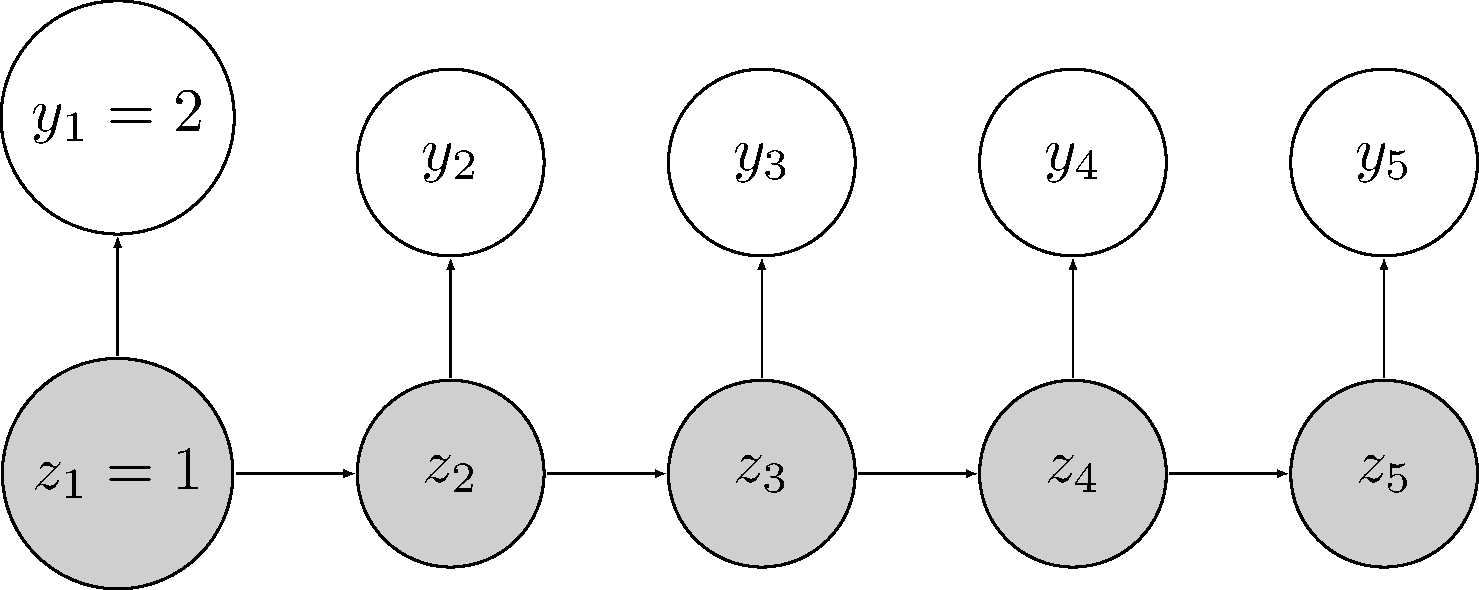
\includegraphics{banana-book_files/figure-latex/unnamed-chunk-131-1.pdf}

States \(z\) are in gray. Observations \(y\) are in white. All individuals are first captured in the first winter \(t = 1\), and are therefore all alive \(z_1 = 1\) and detected \(y_1 = 2\).

\begin{rmdnote}
A hidden Markov model is just two time series running in parallel. One for the states with the Markovian property, and the other of for the observations generated from the states\footnote{HMM are a special case of state-space models in which latent states are discrete.}.
\end{rmdnote}

Have a look to the example below, in which an individual is detected at first sampling occasion, detected again, then missed for the rest of the study. While on occasion \(t=3\) that individual was alive \(z_3=1\) and went undetected \(y_3=1\), on occasions \(t=4\) and \(t=5\) it went undetected \(y_4=y_5=1\) because it was dead \(z_4=z_5=2\).

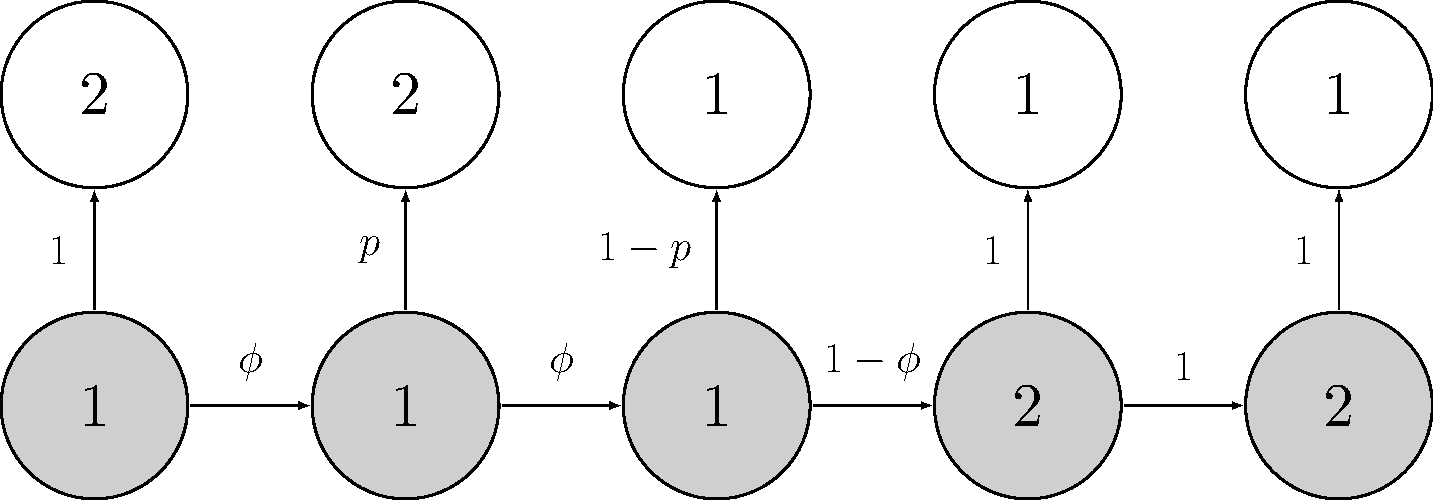
\includegraphics{banana-book_files/figure-latex/unnamed-chunk-132-1.pdf}

\hypertarget{likelihoodhmm}{%
\subsection{Likelihood}\label{likelihoodhmm}}

In the Bayesian framework, we usually work with the so-called complete likelihood, that is the probability of the observed data \(y\) and the latent states \(z\) given the parameters of our model, here the survival and detection probabilities \(\phi\) and \(p\). The complete likelihood for individual \(i\) is:

\begin{align*}
\Pr(\mathbf{y}_i, \mathbf{z}_i) &= \Pr(y_{i,1}, y_{i,2}, \ldots, y_{i,T}, z_{i,1}, z_{i,2}, \ldots, z_{i,T})\\
\end{align*}

Using the definition of a conditional probability, we have:

\begin{align*}
\Pr(\mathbf{y}_i, \mathbf{z}_i) &= \Pr(y_{i,1}, y_{i,2}, \ldots, y_{i,T}, z_{i,1}, z_{i,2}, \ldots, z_{i,T})\\
                  &= \color{blue}{\Pr(y_{i,1}, y_{i,2}, \ldots, y_{i,T} | z_{i,1}, z_{i,2}, \ldots, z_{i,T}) \Pr(z_{i,1}, z_{i,2}, \ldots, z_{i,T})}\\
\end{align*}

Then by using the independence of the \(y\) conditional on the \(z\), and the likelihood of a Markov chain, we get that:

\begin{align*}
\Pr(\mathbf{y}_i, \mathbf{z}_i) &= \Pr(y_{i,1}, y_{i,2}, \ldots, y_{i,T}, z_{i,1}, z_{i,2}, \ldots, z_{i,T})\\
                  &= \Pr(y_{i,1}, y_{i,2}, \ldots, y_{i,T} | z_{i,1}, z_{i,2}, \ldots, z_{i,T}) \Pr(z_{i,1}, z_{i,2}, \ldots, z_{i,T})\\
                &= \color{blue}{\left(\prod_{t=1}^T{\Pr{(y_{i,t} | z_{i,t})}}\right) \left(\Pr(z_{i,1}) \prod_{t=2}^T{\Pr{(z_{i,t} | z_{i,t-1})}}\right)}\\
\end{align*}

Finally, by recognizing the observation and transition probabilities, we have that the complete likelihood for individual \(i\) is:

\begin{align*}
\Pr(\mathbf{y}_i, \mathbf{z}_i) &= \Pr(y_{i,1}, y_{i,2}, \ldots, y_{i,T}, z_{i,1}, z_{i,2}, \ldots, z_{i,T})\\
                  &= \Pr(y_{i,1}, y_{i,2}, \ldots, y_{i,T} | z_{i,1}, z_{i,2}, \ldots, z_{i,T}) \Pr(z_{i,1}, z_{i,2}, \ldots, z_{i,T})\\
                &= \color{blue}{\left(\prod_{t=1}^T{\omega_{z_{i,t}, y_{i,t}}}\right) \left(\Pr(z_{i,1}) \prod_{t=2}^T{\gamma_{z_{i,t-1},z_{i,t}}}\right)}\\
\end{align*}

To obtain the complete likelihood of the whole dataset, we need to multiply this individual likelihood for each animal \(\displaystyle{\prod_{i=1}^N{\Pr(\mathbf{y}_i,\mathbf{z}_i)}}\). When several individuals have the same contribution, calculating their individual contribution only once can greatly reduce the computational burden, as illustrated in Section \ref{pooled-likelihood}.

The Bayesian approach with MCMC methods allows treating the latent states \(z_{i,t}\) as if they were parameters, and to be estimated as such. However, the likelihood is rather complex with a large number of latent states \(z_{i,t}\), which comes with computational costs and slow mixing. There are situations where the latent states are the focus of ecological inference and need to be estimated (see Suggested reading below). However, if not needed, you might want to get rid of the latent states and rely on the so-called marginal likelihood. By doing so, you can avoid sampling the latent states, focus on the ecological parameters, and often speeds up computations and improves mixing as shown in Section \ref{marginalization}. Actually, you can even estimate the latent states afterwards, as illustrated in Section \ref{decoding}.

\hypertarget{fitting-hmm-with-nimble}{%
\section{Fitting HMM with NIMBLE}\label{fitting-hmm-with-nimble}}

Our model so far is written as follows:

\begin{align*}
   z_{\text{first}} &\sim \text{Categorical}(1, \delta) &\text{[likelihood]}\\
   z_t | z_{t-1} &\sim \text{Categorical}(1, \gamma_{z_{t-1},z_{t}}) &\text{[likelihood]}\\
   y_t | z_{t} &\sim \text{Categorical}(1, \omega_{z_{t}}) &\text{[likelihood]}\\
  \phi &\sim \text{Beta}(1, 1) &\text{[prior for }\phi \text{]} \\
  p &\sim \text{Beta}(1, 1) &\text{[prior for }p \text{]} \\
\end{align*}

It has an observation layer for the \(y\)'s, conditional on the \(z\)'s. We also consider uniform priors for the detection and survival probabilities. How to implement this model in NIMBLE?

We start with priors for survival and detection probabilities:

\begin{Shaded}
\begin{Highlighting}[]
\NormalTok{hmm.survival }\OtherTok{\textless{}{-}} \FunctionTok{nimbleCode}\NormalTok{(\{}
\NormalTok{  phi }\SpecialCharTok{\textasciitilde{}} \FunctionTok{dunif}\NormalTok{(}\DecValTok{0}\NormalTok{, }\DecValTok{1}\NormalTok{) }\CommentTok{\# prior survival}
\NormalTok{  p }\SpecialCharTok{\textasciitilde{}} \FunctionTok{dunif}\NormalTok{(}\DecValTok{0}\NormalTok{, }\DecValTok{1}\NormalTok{) }\CommentTok{\# prior detection}
\NormalTok{...}
\end{Highlighting}
\end{Shaded}

Then we define initial states, transition and observation matrices:

\begin{Shaded}
\begin{Highlighting}[]
\NormalTok{...}
  \CommentTok{\# parameters}
\NormalTok{  delta[}\DecValTok{1}\NormalTok{] }\OtherTok{\textless{}{-}} \DecValTok{1}          \CommentTok{\# Pr(alive t = 1) = 1}
\NormalTok{  delta[}\DecValTok{2}\NormalTok{] }\OtherTok{\textless{}{-}} \DecValTok{0}          \CommentTok{\# Pr(dead t = 1) = 0}
\NormalTok{  gamma[}\DecValTok{1}\NormalTok{,}\DecValTok{1}\NormalTok{] }\OtherTok{\textless{}{-}}\NormalTok{ phi      }\CommentTok{\# Pr(alive t {-}\textgreater{} alive t+1)}
\NormalTok{  gamma[}\DecValTok{1}\NormalTok{,}\DecValTok{2}\NormalTok{] }\OtherTok{\textless{}{-}} \DecValTok{1} \SpecialCharTok{{-}}\NormalTok{ phi  }\CommentTok{\# Pr(alive t {-}\textgreater{} dead t+1)}
\NormalTok{  gamma[}\DecValTok{2}\NormalTok{,}\DecValTok{1}\NormalTok{] }\OtherTok{\textless{}{-}} \DecValTok{0}        \CommentTok{\# Pr(dead t {-}\textgreater{} alive t+1)}
\NormalTok{  gamma[}\DecValTok{2}\NormalTok{,}\DecValTok{2}\NormalTok{] }\OtherTok{\textless{}{-}} \DecValTok{1}        \CommentTok{\# Pr(dead t {-}\textgreater{} dead t+1)}
\NormalTok{  omega[}\DecValTok{1}\NormalTok{,}\DecValTok{1}\NormalTok{] }\OtherTok{\textless{}{-}} \DecValTok{1} \SpecialCharTok{{-}}\NormalTok{ p    }\CommentTok{\# Pr(alive t {-}\textgreater{} non{-}detected t)}
\NormalTok{  omega[}\DecValTok{1}\NormalTok{,}\DecValTok{2}\NormalTok{] }\OtherTok{\textless{}{-}}\NormalTok{ p        }\CommentTok{\# Pr(alive t {-}\textgreater{} detected t)}
\NormalTok{  omega[}\DecValTok{2}\NormalTok{,}\DecValTok{1}\NormalTok{] }\OtherTok{\textless{}{-}} \DecValTok{1}        \CommentTok{\# Pr(dead t {-}\textgreater{} non{-}detected t)}
\NormalTok{  omega[}\DecValTok{2}\NormalTok{,}\DecValTok{2}\NormalTok{] }\OtherTok{\textless{}{-}} \DecValTok{0}        \CommentTok{\# Pr(dead t {-}\textgreater{} detected t)}
\NormalTok{...}
\end{Highlighting}
\end{Shaded}

Then the likelihood:

\begin{Shaded}
\begin{Highlighting}[]
\NormalTok{...}
    \CommentTok{\# likelihood}
    \ControlFlowTok{for}\NormalTok{ (i }\ControlFlowTok{in} \DecValTok{1}\SpecialCharTok{:}\NormalTok{N)\{}
\NormalTok{    z[i,}\DecValTok{1}\NormalTok{] }\SpecialCharTok{\textasciitilde{}} \FunctionTok{dcat}\NormalTok{(delta[}\DecValTok{1}\SpecialCharTok{:}\DecValTok{2}\NormalTok{])}
    \ControlFlowTok{for}\NormalTok{ (j }\ControlFlowTok{in} \DecValTok{2}\SpecialCharTok{:}\NormalTok{T)\{}
\NormalTok{      z[i,j] }\SpecialCharTok{\textasciitilde{}} \FunctionTok{dcat}\NormalTok{(gamma[z[i,j}\DecValTok{{-}1}\NormalTok{], }\DecValTok{1}\SpecialCharTok{:}\DecValTok{2}\NormalTok{])}
\NormalTok{      y[i,j] }\SpecialCharTok{\textasciitilde{}} \FunctionTok{dcat}\NormalTok{(omega[z[i,j], }\DecValTok{1}\SpecialCharTok{:}\DecValTok{2}\NormalTok{])}
\NormalTok{    \}}
\NormalTok{  \}}
\ErrorTok{\})}
\end{Highlighting}
\end{Shaded}

Overall, the code looks like:

\begin{Shaded}
\begin{Highlighting}[]
\NormalTok{hmm.survival }\OtherTok{\textless{}{-}} \FunctionTok{nimbleCode}\NormalTok{(\{}
\NormalTok{  phi }\SpecialCharTok{\textasciitilde{}} \FunctionTok{dunif}\NormalTok{(}\DecValTok{0}\NormalTok{, }\DecValTok{1}\NormalTok{) }\CommentTok{\# prior survival}
\NormalTok{  p }\SpecialCharTok{\textasciitilde{}} \FunctionTok{dunif}\NormalTok{(}\DecValTok{0}\NormalTok{, }\DecValTok{1}\NormalTok{) }\CommentTok{\# prior detection}
  \CommentTok{\# likelihood}
\NormalTok{  delta[}\DecValTok{1}\NormalTok{] }\OtherTok{\textless{}{-}} \DecValTok{1}          \CommentTok{\# Pr(alive t = 1) = 1}
\NormalTok{  delta[}\DecValTok{2}\NormalTok{] }\OtherTok{\textless{}{-}} \DecValTok{0}          \CommentTok{\# Pr(dead t = 1) = 0}
\NormalTok{  gamma[}\DecValTok{1}\NormalTok{,}\DecValTok{1}\NormalTok{] }\OtherTok{\textless{}{-}}\NormalTok{ phi      }\CommentTok{\# Pr(alive t {-}\textgreater{} alive t+1)}
\NormalTok{  gamma[}\DecValTok{1}\NormalTok{,}\DecValTok{2}\NormalTok{] }\OtherTok{\textless{}{-}} \DecValTok{1} \SpecialCharTok{{-}}\NormalTok{ phi  }\CommentTok{\# Pr(alive t {-}\textgreater{} dead t+1)}
\NormalTok{  gamma[}\DecValTok{2}\NormalTok{,}\DecValTok{1}\NormalTok{] }\OtherTok{\textless{}{-}} \DecValTok{0}        \CommentTok{\# Pr(dead t {-}\textgreater{} alive t+1)}
\NormalTok{  gamma[}\DecValTok{2}\NormalTok{,}\DecValTok{2}\NormalTok{] }\OtherTok{\textless{}{-}} \DecValTok{1}        \CommentTok{\# Pr(dead t {-}\textgreater{} dead t+1)}
\NormalTok{  omega[}\DecValTok{1}\NormalTok{,}\DecValTok{1}\NormalTok{] }\OtherTok{\textless{}{-}} \DecValTok{1} \SpecialCharTok{{-}}\NormalTok{ p    }\CommentTok{\# Pr(alive t {-}\textgreater{} non{-}detected t)}
\NormalTok{  omega[}\DecValTok{1}\NormalTok{,}\DecValTok{2}\NormalTok{] }\OtherTok{\textless{}{-}}\NormalTok{ p        }\CommentTok{\# Pr(alive t {-}\textgreater{} detected t)}
\NormalTok{  omega[}\DecValTok{2}\NormalTok{,}\DecValTok{1}\NormalTok{] }\OtherTok{\textless{}{-}} \DecValTok{1}        \CommentTok{\# Pr(dead t {-}\textgreater{} non{-}detected t)}
\NormalTok{  omega[}\DecValTok{2}\NormalTok{,}\DecValTok{2}\NormalTok{] }\OtherTok{\textless{}{-}} \DecValTok{0}        \CommentTok{\# Pr(dead t {-}\textgreater{} detected t)}
  \ControlFlowTok{for}\NormalTok{ (i }\ControlFlowTok{in} \DecValTok{1}\SpecialCharTok{:}\NormalTok{N)\{}
\NormalTok{    z[i,}\DecValTok{1}\NormalTok{] }\SpecialCharTok{\textasciitilde{}} \FunctionTok{dcat}\NormalTok{(delta[}\DecValTok{1}\SpecialCharTok{:}\DecValTok{2}\NormalTok{])}
    \ControlFlowTok{for}\NormalTok{ (j }\ControlFlowTok{in} \DecValTok{2}\SpecialCharTok{:}\NormalTok{T)\{}
\NormalTok{      z[i,j] }\SpecialCharTok{\textasciitilde{}} \FunctionTok{dcat}\NormalTok{(gamma[z[i,j}\DecValTok{{-}1}\NormalTok{], }\DecValTok{1}\SpecialCharTok{:}\DecValTok{2}\NormalTok{])}
\NormalTok{      y[i,j] }\SpecialCharTok{\textasciitilde{}} \FunctionTok{dcat}\NormalTok{(omega[z[i,j], }\DecValTok{1}\SpecialCharTok{:}\DecValTok{2}\NormalTok{])}
\NormalTok{    \}}
\NormalTok{  \}}
\NormalTok{\})}
\end{Highlighting}
\end{Shaded}

Now we specify the constants:

\begin{Shaded}
\begin{Highlighting}[]
\NormalTok{my.constants }\OtherTok{\textless{}{-}} \FunctionTok{list}\NormalTok{(}\AttributeTok{N =} \FunctionTok{nrow}\NormalTok{(y), }\AttributeTok{T =} \DecValTok{5}\NormalTok{)}
\NormalTok{my.constants}
\DocumentationTok{\#\# $N}
\DocumentationTok{\#\# [1] 57}
\DocumentationTok{\#\# }
\DocumentationTok{\#\# $T}
\DocumentationTok{\#\# [1] 5}
\end{Highlighting}
\end{Shaded}

The data are made of 0's for non-detections and 1's for detections. To use the categorical distribution, we need to code 1's and 2's. We simply add 1 to get the correct format, that is \(y = 1\) for non-detection and \(y = 2\) for detection: \textbf{Using 1 and 2 would make my life easier\ldots{} The 0/1 coding is a convention; Using the 1/2 coding would make clear that non-detections are actual data (while the use of 0s for non-detections is sometimes confusing). Also, it might help to replace states 1 and 2 by A and D for dead and alive. Even if not mathematically convenient, I guess it would help the understanding. Do it, do it.}

\begin{Shaded}
\begin{Highlighting}[]
\NormalTok{my.data }\OtherTok{\textless{}{-}} \FunctionTok{list}\NormalTok{(}\AttributeTok{y =}\NormalTok{ y }\SpecialCharTok{+} \DecValTok{1}\NormalTok{)}
\end{Highlighting}
\end{Shaded}

Now let's write a function for the initial values:

\begin{Shaded}
\begin{Highlighting}[]
\NormalTok{zinits }\OtherTok{\textless{}{-}}\NormalTok{ y }\SpecialCharTok{+} \DecValTok{1} \CommentTok{\# non{-}detection {-}\textgreater{} alive}
\NormalTok{zinits[zinits }\SpecialCharTok{==} \DecValTok{2}\NormalTok{] }\OtherTok{\textless{}{-}} \DecValTok{1} \CommentTok{\# dead {-}\textgreater{} alive}
\NormalTok{initial.values }\OtherTok{\textless{}{-}} \ControlFlowTok{function}\NormalTok{() }\FunctionTok{list}\NormalTok{(}\AttributeTok{phi =} \FunctionTok{runif}\NormalTok{(}\DecValTok{1}\NormalTok{,}\DecValTok{0}\NormalTok{,}\DecValTok{1}\NormalTok{),}
                                  \AttributeTok{p =} \FunctionTok{runif}\NormalTok{(}\DecValTok{1}\NormalTok{,}\DecValTok{0}\NormalTok{,}\DecValTok{1}\NormalTok{),}
                                  \AttributeTok{z =}\NormalTok{ zinits)}
\end{Highlighting}
\end{Shaded}

We specify the parameters we'd like to monitor:

\begin{Shaded}
\begin{Highlighting}[]
\NormalTok{parameters.to.save }\OtherTok{\textless{}{-}} \FunctionTok{c}\NormalTok{(}\StringTok{"phi"}\NormalTok{, }\StringTok{"p"}\NormalTok{)}
\NormalTok{parameters.to.save}
\DocumentationTok{\#\# [1] "phi" "p"}
\end{Highlighting}
\end{Shaded}

We provide MCMC details:

\begin{Shaded}
\begin{Highlighting}[]
\NormalTok{n.iter }\OtherTok{\textless{}{-}} \DecValTok{5000}
\NormalTok{n.burnin }\OtherTok{\textless{}{-}} \DecValTok{1000}
\NormalTok{n.chains }\OtherTok{\textless{}{-}} \DecValTok{2}
\end{Highlighting}
\end{Shaded}

At last, we're ready to run NIMBLE:

\begin{Shaded}
\begin{Highlighting}[]
\NormalTok{start\_time }\OtherTok{\textless{}{-}} \FunctionTok{Sys.time}\NormalTok{()}
\NormalTok{mcmc.output }\OtherTok{\textless{}{-}} \FunctionTok{nimbleMCMC}\NormalTok{(}\AttributeTok{code =}\NormalTok{ hmm.survival,}
                          \AttributeTok{constants =}\NormalTok{ my.constants,}
                          \AttributeTok{data =}\NormalTok{ my.data,}
                          \AttributeTok{inits =}\NormalTok{ initial.values,}
                          \AttributeTok{monitors =}\NormalTok{ parameters.to.save,}
                          \AttributeTok{niter =}\NormalTok{ n.iter,}
                          \AttributeTok{nburnin =}\NormalTok{ n.burnin,}
                          \AttributeTok{nchains =}\NormalTok{ n.chains)}
\NormalTok{end\_time }\OtherTok{\textless{}{-}} \FunctionTok{Sys.time}\NormalTok{()}
\NormalTok{end\_time }\SpecialCharTok{{-}}\NormalTok{ start\_time}
\end{Highlighting}
\end{Shaded}

\begin{verbatim}
## Time difference of 18.91 secs
\end{verbatim}

We can have a look to numerical summaries:

\begin{Shaded}
\begin{Highlighting}[]
\FunctionTok{MCMCsummary}\NormalTok{(mcmc.output, }\AttributeTok{round =} \DecValTok{2}\NormalTok{)}
\DocumentationTok{\#\#     mean   sd 2.5\%  50\% 97.5\% Rhat n.eff}
\DocumentationTok{\#\# p   0.61 0.06 0.50 0.61  0.72    1   740}
\DocumentationTok{\#\# phi 0.75 0.04 0.67 0.75  0.83    1   805}
\end{Highlighting}
\end{Shaded}

The estimates for survival and detection are close to true survival \(\phi = 0.8\) and detection \(p = 0.6\) with which we simulated the data. The code I used is:

\begin{Shaded}
\begin{Highlighting}[]
\FunctionTok{set.seed}\NormalTok{(}\DecValTok{2022}\NormalTok{) }\CommentTok{\# for reproducibility}
\NormalTok{nocc }\OtherTok{\textless{}{-}} \DecValTok{5} \CommentTok{\# nb of winters or sampling occasions}
\NormalTok{nind }\OtherTok{\textless{}{-}} \DecValTok{57} \CommentTok{\# nb of animals}
\NormalTok{p }\OtherTok{\textless{}{-}} \FloatTok{0.6} \CommentTok{\# detection prob}
\NormalTok{phi }\OtherTok{\textless{}{-}} \FloatTok{0.8} \CommentTok{\# survival prob}
\CommentTok{\# Vector of initial states probabilities}
\NormalTok{delta }\OtherTok{\textless{}{-}} \FunctionTok{c}\NormalTok{(}\DecValTok{1}\NormalTok{,}\DecValTok{0}\NormalTok{) }\CommentTok{\# all individuals are alive in first winter}
\CommentTok{\# Transition matrix}
\NormalTok{Gamma }\OtherTok{\textless{}{-}} \FunctionTok{matrix}\NormalTok{(}\ConstantTok{NA}\NormalTok{, }\DecValTok{2}\NormalTok{, }\DecValTok{2}\NormalTok{)}
\NormalTok{Gamma[}\DecValTok{1}\NormalTok{,}\DecValTok{1}\NormalTok{] }\OtherTok{\textless{}{-}}\NormalTok{ phi      }\CommentTok{\# Pr(alive t {-}\textgreater{} alive t+1)}
\NormalTok{Gamma[}\DecValTok{1}\NormalTok{,}\DecValTok{2}\NormalTok{] }\OtherTok{\textless{}{-}} \DecValTok{1} \SpecialCharTok{{-}}\NormalTok{ phi  }\CommentTok{\# Pr(alive t {-}\textgreater{} dead t+1)}
\NormalTok{Gamma[}\DecValTok{2}\NormalTok{,}\DecValTok{1}\NormalTok{] }\OtherTok{\textless{}{-}} \DecValTok{0}        \CommentTok{\# Pr(dead t {-}\textgreater{} alive t+1)}
\NormalTok{Gamma[}\DecValTok{2}\NormalTok{,}\DecValTok{2}\NormalTok{] }\OtherTok{\textless{}{-}} \DecValTok{1}        \CommentTok{\# Pr(dead t {-}\textgreater{} dead t+1)}
\CommentTok{\# Observation matrix }
\NormalTok{Omega }\OtherTok{\textless{}{-}} \FunctionTok{matrix}\NormalTok{(}\ConstantTok{NA}\NormalTok{, }\DecValTok{2}\NormalTok{, }\DecValTok{2}\NormalTok{)}
\NormalTok{Omega[}\DecValTok{1}\NormalTok{,}\DecValTok{1}\NormalTok{] }\OtherTok{\textless{}{-}} \DecValTok{1} \SpecialCharTok{{-}}\NormalTok{ p      }\CommentTok{\# Pr(alive t {-}\textgreater{} non{-}detected t)}
\NormalTok{Omega[}\DecValTok{1}\NormalTok{,}\DecValTok{2}\NormalTok{] }\OtherTok{\textless{}{-}}\NormalTok{ p          }\CommentTok{\# Pr(alive t {-}\textgreater{} detected t)}
\NormalTok{Omega[}\DecValTok{2}\NormalTok{,}\DecValTok{1}\NormalTok{] }\OtherTok{\textless{}{-}} \DecValTok{1}          \CommentTok{\# Pr(dead t {-}\textgreater{} non{-}detected t)}
\NormalTok{Omega[}\DecValTok{2}\NormalTok{,}\DecValTok{2}\NormalTok{] }\OtherTok{\textless{}{-}} \DecValTok{0}          \CommentTok{\# Pr(dead t {-}\textgreater{} detected t)}
\CommentTok{\# Matrix of states}
\NormalTok{z }\OtherTok{\textless{}{-}} \FunctionTok{matrix}\NormalTok{(}\ConstantTok{NA}\NormalTok{, }\AttributeTok{nrow =}\NormalTok{ nind, }\AttributeTok{ncol =}\NormalTok{ nocc)}
\NormalTok{y }\OtherTok{\textless{}{-}}\NormalTok{ z}
\NormalTok{y[,}\DecValTok{1}\NormalTok{] }\OtherTok{\textless{}{-}} \DecValTok{2} \CommentTok{\# all individuals are detected in first winter}
\ControlFlowTok{for}\NormalTok{ (i }\ControlFlowTok{in} \DecValTok{1}\SpecialCharTok{:}\NormalTok{nind)\{}
\NormalTok{  z[i,}\DecValTok{1}\NormalTok{] }\OtherTok{\textless{}{-}} \FunctionTok{rcat}\NormalTok{(}\AttributeTok{n =} \DecValTok{1}\NormalTok{, }\AttributeTok{prob =}\NormalTok{ delta) }\CommentTok{\# 1 for sure}
  \ControlFlowTok{for}\NormalTok{ (t }\ControlFlowTok{in} \DecValTok{2}\SpecialCharTok{:}\NormalTok{nocc)\{}
    \CommentTok{\# state at t given state at t{-}1}
\NormalTok{    z[i,t] }\OtherTok{\textless{}{-}} \FunctionTok{rcat}\NormalTok{(}\AttributeTok{n =} \DecValTok{1}\NormalTok{, }\AttributeTok{prob =}\NormalTok{ Gamma[z[i,t}\DecValTok{{-}1}\NormalTok{],}\DecValTok{1}\SpecialCharTok{:}\DecValTok{2}\NormalTok{]) }
    \CommentTok{\# observation at t given state at t}
\NormalTok{    y[i,t] }\OtherTok{\textless{}{-}} \FunctionTok{rcat}\NormalTok{(}\AttributeTok{n =} \DecValTok{1}\NormalTok{, }\AttributeTok{prob =}\NormalTok{ Omega[z[i,t],}\DecValTok{1}\SpecialCharTok{:}\DecValTok{2}\NormalTok{]) }
\NormalTok{  \}}
\NormalTok{\}}
\NormalTok{y}
\NormalTok{y }\OtherTok{\textless{}{-}}\NormalTok{ y }\SpecialCharTok{{-}} \DecValTok{1} \CommentTok{\# non{-}detection = 0, detection = 1}
\end{Highlighting}
\end{Shaded}

\hypertarget{marginalization}{%
\section{Marginalization}\label{marginalization}}

In some situations, you will not be interested in inferring the hidden states \(z_{i,t}\), so why bother estimating them? The good news is that you can get rid of the states, so that the marginal likelihood is a function of survival and detection probabilities \(\phi\) and \(p\) only.

\hypertarget{brute-force-approach}{%
\subsection{Brute-force approach}\label{brute-force-approach}}

Using the formula of total probability, you get the marginal likelihood by summing over all possible states in the complete likelihood:

\begin{align*}
\Pr(\mathbf{y}_i) &= \Pr(y_{i,1}, y_{i,2}, \ldots, y_{i,T})\\
                &= \sum_{\mathbf{z}_i} \Pr(\mathbf{y}_i, \mathbf{z}_i)\\
                &= \sum_{z_{i,1}} \cdots \sum_{z_{i,T}} \Pr(y_{i,1}, y_{i,2}, \ldots, y_{i,T}, z_{i,1}, z_{i,2}, \ldots, z_{i,T})\\
\end{align*}

Going through the same steps as for deriving the complete likelihood, we obtain the marginal likelihood:

\begin{align*}
\Pr(\mathbf{y}_i) &= \sum_{z_{i,1}} \cdots \sum_{z_{i,T}} \left(\prod_{t=1}^T{\omega_{z_{i,t}, y_{i,t}}}\right) \left(\Pr(z_{i,1}) \prod_{t=2}^T{\gamma_{z_{i,t-1},z_{i,t}}}\right)\\
\end{align*}

Let's go through an example. Let's imagine we have \(T = 3\) winters, and we'd like to write the likelihood for an individual having the encounter history detected, detected then non-detected. Remember that non-detected is coded 1 and detected is coded 2, while alive is coded 1 and dead is coded 2. We need to calculate \(\Pr(y_1 = 2, y_2 = 2, y_3 = 1)\) which, according to the formula above, is given by:

\begin{align*}
\begin{split}
\Pr(y_1 = 2, y_2 = 2, y_3 = 1) &= \sum_{i=1}^{2} \sum_{j=1}^{2} \sum_{k=1}^{2} \Pr(y_1 = 2 | z_1 = i) \Pr(y_2 = 2 | z_2 = j) \Pr(y_3 = 1 | z_3 = k) \\ 
& \qquad \Pr(z_1=i) \Pr(z_2 = j | z_1 = i) \Pr(z_3 = k | z_2 = j)\\
\end{split}
\end{align*}

Expliciting all the sums in \(\Pr(y_1 = 2, y_2 = 2, y_3 = 1)\), we get the long and ugly expression:

\begin{align*}
\begin{split}
\Pr(y_1 = 2, y_2 = 2, y_3 = 1) &= \\
& \Pr(y_1 = 2 | z_1 = 1) \Pr(y_2 = 2 | z_2 = 1) \Pr(y_3 = 1 | z_3 = 1) \times \\ 
& \qquad \Pr(z_1 = 1) \Pr(z_2 = 1 | z_1 = 1) \Pr(z_3 = 1 | z_2 = 1) +\\
&  \Pr(y_1 = 2 | z_1 = 2) \Pr(y_2 = 2 | z_2 = 1) \Pr(y_3 = 1 | z_3 = 1) \times\\ 
& \qquad \Pr(z_1 = 2) \Pr(z_2 = 1 | z_1 = 2) \Pr(z_3 = 1 | z_2 = 1) +\\
&  \Pr(y_1 = 2 | z_1 = 1) \Pr(y_2 = 2 | z_2 = 2) \Pr(y_3 = 1 | z_3 = 1) \times\\ 
& \qquad \Pr(z_1 = 1) \Pr(z_2 = 2 | z_1 = 1) \Pr(z_3 = 1 | z_2 = 2) +\\
&  \Pr(y_1 = 2 | z_1 = 2) \Pr(y_2 = 2 | z_2 = 2) \Pr(y_3 = 1 | z_3 = 1) \times\\ 
& \qquad \Pr(z_1 = 2) \Pr(z_2 = 2 | z_1 = 2) \Pr(z_3 = 1 | z_2 = 2) +\\
&  \Pr(y_1 = 2 | z_1 = 1) \Pr(y_2 = 2 | z_2 = 1) \Pr(y_3 = 1 | z_3 = 2) \times\\ 
& \qquad \Pr(z_1 = 1) \Pr(z_2 = 1 | z_1 = 1) \Pr(z_3 = 2 | z_2 = 1) +\\
&  \Pr(y_1 = 2 | z_1 = 2) \Pr(y_2 = 2 | z_2 = 1) \Pr(y_3 = 1 | z_3 = 2) \times\\ 
& \qquad \Pr(z_1 = 2) \Pr(z_2 = 1 | z_1 = 2) \Pr(z_3 = 2 | z_2 = 1) +\\
&  \Pr(y_1 = 2 | z_1 = 1) \Pr(y_2 = 2 | z_2 = 2) \Pr(y_3 = 1 | z_3 = 2) \times\\ 
& \qquad \Pr(z_1 = 1) \Pr(z_2 = 2 | z_1 = 1) \Pr(z_3 = 2 | z_2 = 2) +\\
&  \Pr(y_1 = 2 | z_1 = 2) \Pr(y_2 = 2 | z_2 = 2) \Pr(y_3 = 1 | z_3 = 2) \times\\ 
& \qquad \Pr(z_1 = 2) \Pr(z_2 = 2 | z_1 = 2) \Pr(z_3 = 2 | z_2 = 2)\\
\end{split}
\end{align*}

You can simplify this expression by noticing that i) all individuals are alive for sure when marked and released in first winter, or \(\Pr(z_1=2) = 0\) and ii) dead individuals are non-detected for sure, or \(\Pr(y_t = 2|z_t = 2) = 0\), which lead to:

\begin{align*}
\begin{split}
\Pr(y_1 = 2, y_2 = 2, y_3 = 1) &= \\
& \Pr(y_1 = 2 | z_1 = 1) \Pr(y_2 = 2 | z_2 = 1) \Pr(y_3 = 1 | z_3 = 1) \times \\ 
& \qquad \Pr(z_1 = 1) \Pr(z_2 = 1 | z_1 = 1) \Pr(z_3 = 1 | z_2 = 1) +\\
&  \Pr(y_1 = 2 | z_1 = 1) \Pr(y_2 = 2 | z_2 = 1) \Pr(y_3 = 1 | z_3 = 2) \times\\ 
& \qquad \Pr(z_1 = 1) \Pr(z_2 = 1 | z_1 = 1) \Pr(z_3 = 2 | z_2 = 1)\\
\end{split}
\end{align*}

Because all individuals are captured in first winter, or \(\Pr(y_1 = 2 | z_1 = 1) = 1\), we get:

\begin{align*}
\Pr(y_1 = 2, y_2 = 2, y_3 = 1) =  1 (1-p) \times 1 \phi \phi + 1 p 1 \times 1 \phi (1-\phi)
\end{align*}

You end up with \(\Pr(y_1 = 2, y_2 = 2, y_3 = 1) = \phi p (1 - p\phi)\).

The latent states are no longer involved in the likelihood for this individual. However, even on a rather simple example, the marginal likelihood is quite complex to evaluate because it involves many operations. If \(T\) is the length of our encounter histories and \(N\) is the number of hidden states (two for alive and dead, but we will deal with more states in some chapters to come), then we need to calculate the sum of \(N^T\) terms (the sums in the formula above), each of which has two products of \(T\) factors (the products in the formula above), hence \(2TN^T\) calculations in total. You can check that in the simple example above, we have \(T^N = 2^3 = 8\) terms that are summed, each of which is a product of \(2T = 2 \times 3 = 6\) terms. This means that the number of operations increases exponentially as the number of states increases. In most cases, this complexity precludes using this method to get rid of the states. Fortunately, we have another algorithm in the HMM toolbox that is useful to calculate the marginal likelihood efficiently.

\hypertarget{forward-algorithm}{%
\subsection{Forward algorithm}\label{forward-algorithm}}

In the brute-force approach, some products are computed several times to calculate the marginal likelihood. What if we could store these products and use them later while computing the probability of the observation sequence? This is precisely what the forward algorithm does.

We introduce \(\alpha_t(j)\) the probability for the latent state \(z\) of being in state \(j\) at \(t\) after seeing the first \(j\) observations \(y_1, \ldots, y_t\), that is \(\alpha_t(j) = \Pr(y_1, \ldots, y_t, z_t = j)\).

Using the law of total probability, we can write the marginal likelihood as a function of \(\alpha_T(j)\), namely we have \(\Pr(\mathbf{y}) = \displaystyle{\sum_{j=1}^N\Pr(y_1, \ldots, y_t, z_t = j)} = \displaystyle{\sum_{j=1}^N\alpha_T(j)}\).

How to calculate the the \(\alpha_T(j)\)s? This is where the magic of the forward algorithm happens. We use a recurrence relationship that saves us many computations.

The recurrence states that:

\begin{align*}
\alpha_t(j) &= \sum_{i=1}^N \alpha_{t-1}(i) \gamma_{i,j} \omega_{j,y_t}
\end{align*}

How to obtain this recurrence? First, using the law of total probability with \(z_{t-1}\), we have that:
\begin{align*}
\alpha_t(j) &= \sum_{i=1}^N \Pr(y_1, \ldots, y_t, z_{t-1} = i, z_t = j)\\
\end{align*}

Second, using conditional probabilities, we get:
\begin{align*}
\alpha_t(j) &= \sum_{i=1}^N \Pr(y_t | z_{t-1} = i, z_t = j, y_1, \ldots, y_t) \Pr(z_{t-1} = i, z_t = j, y_1, \ldots, y_t)
\end{align*}

Third, using conditional probabilities again, on the second term of the product, we get:
\begin{align*}
\alpha_t(j) &= \sum_{i=1}^N \Pr(y_t | z_{t-1} = i, z_t = j, y_1, \ldots, y_t) \times \\ & \Pr(z_t = j | z_{t-1} = i, y_1, \ldots, y_t) \Pr(z_{t-1} = i, y_1, \ldots, y_t)
\end{align*}

which, using conditional independence, simplifies into:

\begin{align*}
\alpha_t(j) &= \sum_{i=1}^N \Pr(y_t | z_t = j) \Pr(z_t = j | z_{t-1} = i) \Pr(z_{t-1} = i, y_1, \ldots, y_t)
\end{align*}

Recognizing that \(\Pr(y_{t}|z_{t}=j)=\omega_{j,y_t}\), \(\Pr(z_{t} = j | z_{t-1} = i) = \gamma_{i,j}\) and \(\Pr(z_{t-1} = i, y_1, \ldots, y_t) = \alpha_{t-1}(i)\), we obtain the recurrence.

In practice, the forward algorithm works as follows. First you initialize the procedure by calculating for the states \(j=1,\ldots,N\) the quantities \(\alpha_1(j) = Pr(z_1 = j) \omega_{j,y_1}\). Then you compute for the states \(j=1,\ldots,N\) the relationship \(\alpha_t(j) = \displaystyle{\sum_{i=1}^N \alpha_{t-1}(i) \gamma_{i,j} \omega_{j,y_t}}\) for \(t = 2, \ldots, T\). Finally, you compute the marginal likelihood as \(\Pr(\mathbf{y}) = \displaystyle{\sum_{j=1}^N\alpha_T(j)}\). At each time \(t\), we need to calculate \(N\) values of \(\alpha_t(j)\), and each \(\alpha_t(j)\) is a sum of \(N\) products of \(\alpha_{t-1}\), \(\gamma_{i,j}\) and \(\omega_{j,y_t}\), hence \(TN^2\) computations in total, which is much less than the \(2TN^T\) calculations in the brute-force approach.

Going back to our example, we wish to calculate \(\Pr(y_1 = 2, y_2 = 2, y_3 = 1)\). First we initialize and compute \(\alpha_1(1)\) and \(\alpha_1(2)\). We have:

\begin{align*}
\alpha_1(1) = \Pr(z_1=1) \omega_{1,y_1=2} = 1
\end{align*}

because all animals are alive and captured in first winter. We also have:

\begin{align*}
\alpha_1(2) = \Pr(z_1=2) \omega_{2,y_1=2} = 0
\end{align*}

Then we compute \(\alpha_2(1)\) and \(\alpha_2(2)\). We have:

\begin{align*}
\alpha_2(1) &= \sum_{i=1}^2 \alpha_1(i) \gamma_{i,1} \omega_{1,y_2=2}\\
            &= \gamma_{1,1} \omega_{1,y_2=2}\\
            &= \phi p
\end{align*}

because \(\alpha_1(2) = 0\). Also, we have:

\begin{align*}
\alpha_2(2) &= \sum_{i=1}^2 \alpha_1(i) \gamma_{i,2} \omega_{2,y_2=2}\\
            &= \gamma_{1,2} \omega_{2,y_2=2}\\
            &= (1-\phi) 0
\end{align*}

Finally we compute \(\alpha_3(1)\) and \(\alpha_3(2)\). We have:

\begin{align*}
\alpha_3(1) &= \sum_{i=1}^2 \alpha_2(i) \gamma_{i,1} \omega_{1,y_3=1}\\
            &= \alpha_2(1) \gamma_{1,1} \omega_{1,y_3=1}\\
            &= \phi p \phi (1-p)
\end{align*}

and:

\begin{align*}
\alpha_3(2) &= \sum_{i=1}^2 \alpha_2(i) \gamma_{i,2} \omega_{2,y_3=1}\\
            &= \alpha_2(1) \gamma_{1,2} \omega_{2,y_3=1}\\
            &= \phi p (1-\phi) 1
\end{align*}

Eventually, we compute \(\Pr(y_1=2,y_2=2,y_3=1)\):

\begin{align*}
\Pr(y_1=2,y_2=2,y_3=1) &= \alpha_3(1) + \alpha_3(2)\\
            &= \phi p (\phi) (1-p) + \phi p (1-\phi)\\
            &= \phi p (1-\phi p)
\end{align*}

You can check that we did in total \(3 \times 2^2 = 12\) operations.

\hypertarget{nimble-implementation-1}{%
\subsection{NIMBLE implementation}\label{nimble-implementation-1}}

In NIMBLE, we use functions to implement the forward algorithm. The only differences with the theory above is that i) we work on the log scale for numerical stability and ii) we use a matrix formulation of the recurrence.
First we write the density function:

\begin{Shaded}
\begin{Highlighting}[]
\NormalTok{dHMM }\OtherTok{\textless{}{-}} \FunctionTok{nimbleFunction}\NormalTok{(}
  \AttributeTok{run =} \ControlFlowTok{function}\NormalTok{(}\AttributeTok{x =} \FunctionTok{double}\NormalTok{(}\DecValTok{1}\NormalTok{), }
                 \AttributeTok{probInit =} \FunctionTok{double}\NormalTok{(}\DecValTok{1}\NormalTok{),}
                 \AttributeTok{probObs =} \FunctionTok{double}\NormalTok{(}\DecValTok{2}\NormalTok{),}
                 \AttributeTok{probTrans =} \FunctionTok{double}\NormalTok{(}\DecValTok{2}\NormalTok{),}
                 \AttributeTok{len =} \FunctionTok{double}\NormalTok{(}\DecValTok{0}\NormalTok{, }\AttributeTok{default =} \DecValTok{0}\NormalTok{),}
                 \AttributeTok{log =} \FunctionTok{integer}\NormalTok{(}\DecValTok{0}\NormalTok{, }\AttributeTok{default =} \DecValTok{0}\NormalTok{)) \{}
\NormalTok{    alpha }\OtherTok{\textless{}{-}}\NormalTok{ probInit[}\DecValTok{1}\SpecialCharTok{:}\DecValTok{2}\NormalTok{]}
    \ControlFlowTok{for}\NormalTok{ (t }\ControlFlowTok{in} \DecValTok{2}\SpecialCharTok{:}\NormalTok{len) \{}
\NormalTok{      alpha[}\DecValTok{1}\SpecialCharTok{:}\DecValTok{2}\NormalTok{] }\OtherTok{\textless{}{-}}\NormalTok{ (alpha[}\DecValTok{1}\SpecialCharTok{:}\DecValTok{2}\NormalTok{] }\SpecialCharTok{\%*\%}\NormalTok{ probTrans[}\DecValTok{1}\SpecialCharTok{:}\DecValTok{2}\NormalTok{,}\DecValTok{1}\SpecialCharTok{:}\DecValTok{2}\NormalTok{]) }\SpecialCharTok{*}\NormalTok{ probObs[}\DecValTok{1}\SpecialCharTok{:}\DecValTok{2}\NormalTok{,x[t]]}
\NormalTok{    \}}
\NormalTok{    logL }\OtherTok{\textless{}{-}} \FunctionTok{log}\NormalTok{(}\FunctionTok{sum}\NormalTok{(alpha[}\DecValTok{1}\SpecialCharTok{:}\DecValTok{2}\NormalTok{]))}
    \FunctionTok{returnType}\NormalTok{(}\FunctionTok{double}\NormalTok{(}\DecValTok{0}\NormalTok{))}
    \ControlFlowTok{if}\NormalTok{ (log) }\FunctionTok{return}\NormalTok{(logL)}
    \FunctionTok{return}\NormalTok{(}\FunctionTok{exp}\NormalTok{(logL))}
\NormalTok{  \}}
\NormalTok{)}
\end{Highlighting}
\end{Shaded}

In passing, this is the function you would maximize in a Frequentist approach\footnote{I might add that example in a footnote. See also Section \ref{under-the-hood}}. Then we write a function to simulate values from a HMM:

\begin{Shaded}
\begin{Highlighting}[]
\NormalTok{rHMM }\OtherTok{\textless{}{-}} \FunctionTok{nimbleFunction}\NormalTok{(}
  \AttributeTok{run =} \ControlFlowTok{function}\NormalTok{(}\AttributeTok{n =} \FunctionTok{integer}\NormalTok{(),}
                 \AttributeTok{probInit =} \FunctionTok{double}\NormalTok{(}\DecValTok{1}\NormalTok{),}
                 \AttributeTok{probObs =} \FunctionTok{double}\NormalTok{(}\DecValTok{2}\NormalTok{),}
                 \AttributeTok{probTrans =} \FunctionTok{double}\NormalTok{(}\DecValTok{2}\NormalTok{),}
                 \AttributeTok{len =} \FunctionTok{double}\NormalTok{(}\DecValTok{0}\NormalTok{, }\AttributeTok{default =} \DecValTok{0}\NormalTok{)) \{}
    \FunctionTok{returnType}\NormalTok{(}\FunctionTok{double}\NormalTok{(}\DecValTok{1}\NormalTok{))}
\NormalTok{    z }\OtherTok{\textless{}{-}} \FunctionTok{numeric}\NormalTok{(len)}
\NormalTok{    z[}\DecValTok{1}\NormalTok{] }\OtherTok{\textless{}{-}} \FunctionTok{rcat}\NormalTok{(}\AttributeTok{n =} \DecValTok{1}\NormalTok{, }\AttributeTok{prob =}\NormalTok{ probInit[}\DecValTok{1}\SpecialCharTok{:}\DecValTok{2}\NormalTok{]) }\CommentTok{\# all individuals alive at t = 0}
\NormalTok{    y }\OtherTok{\textless{}{-}}\NormalTok{ z}
\NormalTok{    y[}\DecValTok{1}\NormalTok{] }\OtherTok{\textless{}{-}} \DecValTok{2} \CommentTok{\# all individuals are detected at t = 0}
    \ControlFlowTok{for}\NormalTok{ (t }\ControlFlowTok{in} \DecValTok{2}\SpecialCharTok{:}\NormalTok{len)\{}
      \CommentTok{\# state at t given state at t{-}1}
\NormalTok{      z[t] }\OtherTok{\textless{}{-}} \FunctionTok{rcat}\NormalTok{(}\AttributeTok{n =} \DecValTok{1}\NormalTok{, }\AttributeTok{prob =}\NormalTok{ probTrans[z[t}\DecValTok{{-}1}\NormalTok{],}\DecValTok{1}\SpecialCharTok{:}\DecValTok{2}\NormalTok{]) }
      \CommentTok{\# observation at t given state at t}
\NormalTok{      y[t] }\OtherTok{\textless{}{-}} \FunctionTok{rcat}\NormalTok{(}\AttributeTok{n =} \DecValTok{1}\NormalTok{, }\AttributeTok{prob =}\NormalTok{ probObs[z[t],}\DecValTok{1}\SpecialCharTok{:}\DecValTok{2}\NormalTok{]) }
\NormalTok{    \}}
    \FunctionTok{return}\NormalTok{(y)}
\NormalTok{  \})}
\end{Highlighting}
\end{Shaded}

We assign these functions to the global R environment:

\begin{Shaded}
\begin{Highlighting}[]
\FunctionTok{assign}\NormalTok{(}\StringTok{\textquotesingle{}dHMM\textquotesingle{}}\NormalTok{, dHMM, .GlobalEnv)}
\FunctionTok{assign}\NormalTok{(}\StringTok{\textquotesingle{}rHMM\textquotesingle{}}\NormalTok{, rHMM, .GlobalEnv)}
\end{Highlighting}
\end{Shaded}

Now we resume our workflow:

\begin{Shaded}
\begin{Highlighting}[]
\CommentTok{\# code}
\NormalTok{hmm.survival }\OtherTok{\textless{}{-}} \FunctionTok{nimbleCode}\NormalTok{(\{}
\NormalTok{  phi }\SpecialCharTok{\textasciitilde{}} \FunctionTok{dunif}\NormalTok{(}\DecValTok{0}\NormalTok{, }\DecValTok{1}\NormalTok{) }\CommentTok{\# prior survival}
\NormalTok{  p }\SpecialCharTok{\textasciitilde{}} \FunctionTok{dunif}\NormalTok{(}\DecValTok{0}\NormalTok{, }\DecValTok{1}\NormalTok{) }\CommentTok{\# prior detection}
  \CommentTok{\# likelihood}
\NormalTok{  delta[}\DecValTok{1}\NormalTok{] }\OtherTok{\textless{}{-}} \DecValTok{1}          \CommentTok{\# Pr(alive t = 1) = 1}
\NormalTok{  delta[}\DecValTok{2}\NormalTok{] }\OtherTok{\textless{}{-}} \DecValTok{0}          \CommentTok{\# Pr(dead t = 1) = 0}
\NormalTok{  gamma[}\DecValTok{1}\NormalTok{,}\DecValTok{1}\NormalTok{] }\OtherTok{\textless{}{-}}\NormalTok{ phi      }\CommentTok{\# Pr(alive t {-}\textgreater{} alive t+1)}
\NormalTok{  gamma[}\DecValTok{1}\NormalTok{,}\DecValTok{2}\NormalTok{] }\OtherTok{\textless{}{-}} \DecValTok{1} \SpecialCharTok{{-}}\NormalTok{ phi  }\CommentTok{\# Pr(alive t {-}\textgreater{} dead t+1)}
\NormalTok{  gamma[}\DecValTok{2}\NormalTok{,}\DecValTok{1}\NormalTok{] }\OtherTok{\textless{}{-}} \DecValTok{0}        \CommentTok{\# Pr(dead t {-}\textgreater{} alive t+1)}
\NormalTok{  gamma[}\DecValTok{2}\NormalTok{,}\DecValTok{2}\NormalTok{] }\OtherTok{\textless{}{-}} \DecValTok{1}        \CommentTok{\# Pr(dead t {-}\textgreater{} dead t+1)}
\NormalTok{  omega[}\DecValTok{1}\NormalTok{,}\DecValTok{1}\NormalTok{] }\OtherTok{\textless{}{-}} \DecValTok{1} \SpecialCharTok{{-}}\NormalTok{ p    }\CommentTok{\# Pr(alive t {-}\textgreater{} non{-}detected t)}
\NormalTok{  omega[}\DecValTok{1}\NormalTok{,}\DecValTok{2}\NormalTok{] }\OtherTok{\textless{}{-}}\NormalTok{ p        }\CommentTok{\# Pr(alive t {-}\textgreater{} detected t)}
\NormalTok{  omega[}\DecValTok{2}\NormalTok{,}\DecValTok{1}\NormalTok{] }\OtherTok{\textless{}{-}} \DecValTok{1}        \CommentTok{\# Pr(dead t {-}\textgreater{} non{-}detected t)}
\NormalTok{  omega[}\DecValTok{2}\NormalTok{,}\DecValTok{2}\NormalTok{] }\OtherTok{\textless{}{-}} \DecValTok{0}        \CommentTok{\# Pr(dead t {-}\textgreater{} detected t)}
  \ControlFlowTok{for}\NormalTok{ (i }\ControlFlowTok{in} \DecValTok{1}\SpecialCharTok{:}\NormalTok{N)\{}
\NormalTok{    y[i,}\DecValTok{1}\SpecialCharTok{:}\NormalTok{T] }\SpecialCharTok{\textasciitilde{}} \FunctionTok{dHMM}\NormalTok{(}\AttributeTok{probInit =}\NormalTok{ delta[}\DecValTok{1}\SpecialCharTok{:}\DecValTok{2}\NormalTok{], }
                    \AttributeTok{probObs =}\NormalTok{ omega[}\DecValTok{1}\SpecialCharTok{:}\DecValTok{2}\NormalTok{,}\DecValTok{1}\SpecialCharTok{:}\DecValTok{2}\NormalTok{], }\CommentTok{\# observation matrix}
                    \AttributeTok{probTrans =}\NormalTok{ gamma[}\DecValTok{1}\SpecialCharTok{:}\DecValTok{2}\NormalTok{,}\DecValTok{1}\SpecialCharTok{:}\DecValTok{2}\NormalTok{], }\CommentTok{\# transition matrix}
                    \AttributeTok{len =}\NormalTok{ T) }\CommentTok{\# nb of sampling occasions}
\NormalTok{  \}}
\NormalTok{\})}
\CommentTok{\# constants}
\NormalTok{my.constants }\OtherTok{\textless{}{-}} \FunctionTok{list}\NormalTok{(}\AttributeTok{N =} \FunctionTok{nrow}\NormalTok{(y), }\AttributeTok{T =} \DecValTok{5}\NormalTok{)}
\CommentTok{\# data}
\NormalTok{my.data }\OtherTok{\textless{}{-}} \FunctionTok{list}\NormalTok{(}\AttributeTok{y =}\NormalTok{ y }\SpecialCharTok{+} \DecValTok{1}\NormalTok{)}
\CommentTok{\# initial values {-} no need to specify values for z anymore}
\NormalTok{initial.values }\OtherTok{\textless{}{-}} \ControlFlowTok{function}\NormalTok{() }\FunctionTok{list}\NormalTok{(}\AttributeTok{phi =} \FunctionTok{runif}\NormalTok{(}\DecValTok{1}\NormalTok{,}\DecValTok{0}\NormalTok{,}\DecValTok{1}\NormalTok{),}
                                  \AttributeTok{p =} \FunctionTok{runif}\NormalTok{(}\DecValTok{1}\NormalTok{,}\DecValTok{0}\NormalTok{,}\DecValTok{1}\NormalTok{))}
\CommentTok{\# parameters to save}
\NormalTok{parameters.to.save }\OtherTok{\textless{}{-}} \FunctionTok{c}\NormalTok{(}\StringTok{"phi"}\NormalTok{, }\StringTok{"p"}\NormalTok{)}
\CommentTok{\# MCMC details}
\NormalTok{n.iter }\OtherTok{\textless{}{-}} \DecValTok{5000}
\NormalTok{n.burnin }\OtherTok{\textless{}{-}} \DecValTok{1000}
\NormalTok{n.chains }\OtherTok{\textless{}{-}} \DecValTok{2}
\end{Highlighting}
\end{Shaded}

And run NIMBLE:

\begin{Shaded}
\begin{Highlighting}[]
\NormalTok{start\_time }\OtherTok{\textless{}{-}} \FunctionTok{Sys.time}\NormalTok{()}
\NormalTok{mcmc.output }\OtherTok{\textless{}{-}} \FunctionTok{nimbleMCMC}\NormalTok{(}\AttributeTok{code =}\NormalTok{ hmm.survival,}
                          \AttributeTok{constants =}\NormalTok{ my.constants,}
                          \AttributeTok{data =}\NormalTok{ my.data,}
                          \AttributeTok{inits =}\NormalTok{ initial.values,}
                          \AttributeTok{monitors =}\NormalTok{ parameters.to.save,}
                          \AttributeTok{niter =}\NormalTok{ n.iter,}
                          \AttributeTok{nburnin =}\NormalTok{ n.burnin,}
                          \AttributeTok{nchains =}\NormalTok{ n.chains)}
\DocumentationTok{\#\# |{-}{-}{-}{-}{-}{-}{-}{-}{-}{-}{-}{-}{-}|{-}{-}{-}{-}{-}{-}{-}{-}{-}{-}{-}{-}{-}|{-}{-}{-}{-}{-}{-}{-}{-}{-}{-}{-}{-}{-}|{-}{-}{-}{-}{-}{-}{-}{-}{-}{-}{-}{-}{-}|}
\DocumentationTok{\#\# |{-}{-}{-}{-}{-}{-}{-}{-}{-}{-}{-}{-}{-}{-}{-}{-}{-}{-}{-}{-}{-}{-}{-}{-}{-}{-}{-}{-}{-}{-}{-}{-}{-}{-}{-}{-}{-}{-}{-}{-}{-}{-}{-}{-}{-}{-}{-}{-}{-}{-}{-}{-}{-}{-}{-}|}
\DocumentationTok{\#\# |{-}{-}{-}{-}{-}{-}{-}{-}{-}{-}{-}{-}{-}|{-}{-}{-}{-}{-}{-}{-}{-}{-}{-}{-}{-}{-}|{-}{-}{-}{-}{-}{-}{-}{-}{-}{-}{-}{-}{-}|{-}{-}{-}{-}{-}{-}{-}{-}{-}{-}{-}{-}{-}|}
\DocumentationTok{\#\# |{-}{-}{-}{-}{-}{-}{-}{-}{-}{-}{-}{-}{-}{-}{-}{-}{-}{-}{-}{-}{-}{-}{-}{-}{-}{-}{-}{-}{-}{-}{-}{-}{-}{-}{-}{-}{-}{-}{-}{-}{-}{-}{-}{-}{-}{-}{-}{-}{-}{-}{-}{-}{-}{-}{-}|}
\NormalTok{end\_time }\OtherTok{\textless{}{-}} \FunctionTok{Sys.time}\NormalTok{()}
\NormalTok{end\_time }\SpecialCharTok{{-}}\NormalTok{ start\_time}
\DocumentationTok{\#\# Time difference of 18.18 secs}
\end{Highlighting}
\end{Shaded}

The numerical summaries are similar to those we obtained with the complete likelihood, and effective samples sizes are larger denoting better mixing:

\begin{Shaded}
\begin{Highlighting}[]
\FunctionTok{MCMCsummary}\NormalTok{(mcmc.output, }\AttributeTok{round =} \DecValTok{2}\NormalTok{)}
\DocumentationTok{\#\#     mean   sd 2.5\%  50\% 97.5\% Rhat n.eff}
\DocumentationTok{\#\# p   0.61 0.06 0.49 0.61  0.72    1  1211}
\DocumentationTok{\#\# phi 0.76 0.04 0.67 0.76  0.84    1  1483}
\end{Highlighting}
\end{Shaded}

\hypertarget{pooled-likelihood}{%
\section{Pooled encounter histories}\label{pooled-likelihood}}

We can go one step further to make convergence even faster. As mentionned earlier in Section \ref{likelihoodhmm}, the likelihood of an HMM fitted to capture-recapture data often involves individuals that share the same encounter histories. Instead of repeating the same calculations several times, the likelihood contribution that is shared by say \(x\) individuals is raised to the power \(x\) in the likelihood of the whole dataset, hence making the same operations only once\footnote{This idea is used in routine in capture-recapture software like MARK or E-SURGE. For Bayesian software however, it is only recently that the trick was tested in NIMBLE (in Turek, de Valpine, and Paciorek (2016). Efficient Markov chain Monte Carlo sampling for hierarchical hidden Markov models. \emph{Environmental and Ecological Statistics} 23: 549-564. Many thanks to Chloé Nater for showing me how to implement it.}.

In this section, we amend the NIMBLE functions we wrote for marginalizing latent states in Section \ref{marginalization} to express the likelihood using pooled encounter histories. We use a vector \texttt{size} that contains the number of individuals with the same encounter history.

The density function is the function \texttt{dHMM} to which we add a \texttt{size} argument, and raise the individual likelihood to the power \texttt{size}, or multiply by \texttt{size} as we work on the log scale \texttt{log(sum(alpha{[}1:2{]}))\ *\ size}:

\begin{Shaded}
\begin{Highlighting}[]
\NormalTok{dHMMpooled }\OtherTok{\textless{}{-}} \FunctionTok{nimbleFunction}\NormalTok{(}
  \AttributeTok{run =} \ControlFlowTok{function}\NormalTok{(}\AttributeTok{x =} \FunctionTok{double}\NormalTok{(}\DecValTok{1}\NormalTok{), }
                 \AttributeTok{probInit =} \FunctionTok{double}\NormalTok{(}\DecValTok{1}\NormalTok{),}
                 \AttributeTok{probObs =} \FunctionTok{double}\NormalTok{(}\DecValTok{2}\NormalTok{),}
                 \AttributeTok{probTrans =} \FunctionTok{double}\NormalTok{(}\DecValTok{2}\NormalTok{),}
                 \AttributeTok{len =} \FunctionTok{double}\NormalTok{(}\DecValTok{0}\NormalTok{),}
                 \AttributeTok{size =} \FunctionTok{double}\NormalTok{(}\DecValTok{0}\NormalTok{),}
                 \AttributeTok{log =} \FunctionTok{integer}\NormalTok{(}\DecValTok{0}\NormalTok{, }\AttributeTok{default =} \DecValTok{0}\NormalTok{)) \{}
\NormalTok{    alpha }\OtherTok{\textless{}{-}}\NormalTok{ probInit[}\DecValTok{1}\SpecialCharTok{:}\DecValTok{2}\NormalTok{]}
    \ControlFlowTok{for}\NormalTok{ (t }\ControlFlowTok{in} \DecValTok{2}\SpecialCharTok{:}\NormalTok{len) \{}
\NormalTok{      alpha[}\DecValTok{1}\SpecialCharTok{:}\DecValTok{2}\NormalTok{] }\OtherTok{\textless{}{-}}\NormalTok{ (alpha[}\DecValTok{1}\SpecialCharTok{:}\DecValTok{2}\NormalTok{] }\SpecialCharTok{\%*\%}\NormalTok{ probTrans[}\DecValTok{1}\SpecialCharTok{:}\DecValTok{2}\NormalTok{,}\DecValTok{1}\SpecialCharTok{:}\DecValTok{2}\NormalTok{]) }\SpecialCharTok{*}\NormalTok{ probObs[}\DecValTok{1}\SpecialCharTok{:}\DecValTok{2}\NormalTok{,x[t]]}
\NormalTok{    \}}
\NormalTok{    logL }\OtherTok{\textless{}{-}} \FunctionTok{log}\NormalTok{(}\FunctionTok{sum}\NormalTok{(alpha[}\DecValTok{1}\SpecialCharTok{:}\DecValTok{2}\NormalTok{])) }\SpecialCharTok{*}\NormalTok{ size}
    \FunctionTok{returnType}\NormalTok{(}\FunctionTok{double}\NormalTok{(}\DecValTok{0}\NormalTok{))}
    \ControlFlowTok{if}\NormalTok{ (log) }\FunctionTok{return}\NormalTok{(logL)}
    \FunctionTok{return}\NormalTok{(}\FunctionTok{exp}\NormalTok{(logL))}
\NormalTok{  \}}
\NormalTok{)}
\end{Highlighting}
\end{Shaded}

The \texttt{rHMM} function is renamed \texttt{rHMMpooled} for compatibility but remains unchanged:

\begin{Shaded}
\begin{Highlighting}[]
\NormalTok{rHMMpooled }\OtherTok{\textless{}{-}} \FunctionTok{nimbleFunction}\NormalTok{(}
  \AttributeTok{run =} \ControlFlowTok{function}\NormalTok{(}\AttributeTok{n =} \FunctionTok{integer}\NormalTok{(),}
                 \AttributeTok{probInit =} \FunctionTok{double}\NormalTok{(}\DecValTok{1}\NormalTok{),}
                 \AttributeTok{probObs =} \FunctionTok{double}\NormalTok{(}\DecValTok{2}\NormalTok{),}
                 \AttributeTok{probTrans =} \FunctionTok{double}\NormalTok{(}\DecValTok{2}\NormalTok{),}
                 \AttributeTok{len =} \FunctionTok{double}\NormalTok{(}\DecValTok{0}\NormalTok{),}
                 \AttributeTok{size =} \FunctionTok{double}\NormalTok{(}\DecValTok{0}\NormalTok{)) \{}
    \FunctionTok{returnType}\NormalTok{(}\FunctionTok{double}\NormalTok{(}\DecValTok{1}\NormalTok{))}
\NormalTok{    z }\OtherTok{\textless{}{-}} \FunctionTok{numeric}\NormalTok{(len)}
\NormalTok{    z[}\DecValTok{1}\NormalTok{] }\OtherTok{\textless{}{-}} \FunctionTok{rcat}\NormalTok{(}\AttributeTok{n =} \DecValTok{1}\NormalTok{, }\AttributeTok{prob =}\NormalTok{ probInit[}\DecValTok{1}\SpecialCharTok{:}\DecValTok{2}\NormalTok{]) }\CommentTok{\# all individuals alive at t = 0}
\NormalTok{    y }\OtherTok{\textless{}{-}}\NormalTok{ z}
\NormalTok{    y[}\DecValTok{1}\NormalTok{] }\OtherTok{\textless{}{-}} \DecValTok{2} \CommentTok{\# all individuals are detected at t = 0}
    \ControlFlowTok{for}\NormalTok{ (t }\ControlFlowTok{in} \DecValTok{2}\SpecialCharTok{:}\NormalTok{len)\{}
      \CommentTok{\# state at t given state at t{-}1}
\NormalTok{      z[t] }\OtherTok{\textless{}{-}} \FunctionTok{rcat}\NormalTok{(}\AttributeTok{n =} \DecValTok{1}\NormalTok{, }\AttributeTok{prob =}\NormalTok{ probTrans[z[t}\DecValTok{{-}1}\NormalTok{],}\DecValTok{1}\SpecialCharTok{:}\DecValTok{2}\NormalTok{]) }
      \CommentTok{\# observation at t given state at t}
\NormalTok{      y[t] }\OtherTok{\textless{}{-}} \FunctionTok{rcat}\NormalTok{(}\AttributeTok{n =} \DecValTok{1}\NormalTok{, }\AttributeTok{prob =}\NormalTok{ probObs[z[t],}\DecValTok{1}\SpecialCharTok{:}\DecValTok{2}\NormalTok{]) }
\NormalTok{    \}}
    \FunctionTok{return}\NormalTok{(y)}
\NormalTok{  \})}
\end{Highlighting}
\end{Shaded}

We assign these two function to the global R environment so that we can use them:

\begin{Shaded}
\begin{Highlighting}[]
\FunctionTok{assign}\NormalTok{(}\StringTok{\textquotesingle{}dHMMpooled\textquotesingle{}}\NormalTok{, dHMMpooled, .GlobalEnv)}
\FunctionTok{assign}\NormalTok{(}\StringTok{\textquotesingle{}rHMMpooled\textquotesingle{}}\NormalTok{, rHMMpooled, .GlobalEnv)}
\end{Highlighting}
\end{Shaded}

You can now plug your pooled HMM density function in your NIMBLE code:

\begin{Shaded}
\begin{Highlighting}[]
\NormalTok{hmm.survival }\OtherTok{\textless{}{-}} \FunctionTok{nimbleCode}\NormalTok{(\{}
\NormalTok{  phi }\SpecialCharTok{\textasciitilde{}} \FunctionTok{dunif}\NormalTok{(}\DecValTok{0}\NormalTok{, }\DecValTok{1}\NormalTok{) }\CommentTok{\# prior survival}
\NormalTok{  p }\SpecialCharTok{\textasciitilde{}} \FunctionTok{dunif}\NormalTok{(}\DecValTok{0}\NormalTok{, }\DecValTok{1}\NormalTok{) }\CommentTok{\# prior detection}
  \CommentTok{\# likelihood}
\NormalTok{  delta[}\DecValTok{1}\NormalTok{] }\OtherTok{\textless{}{-}} \DecValTok{1}          \CommentTok{\# Pr(alive t = 1) = 1}
\NormalTok{  delta[}\DecValTok{2}\NormalTok{] }\OtherTok{\textless{}{-}} \DecValTok{0}          \CommentTok{\# Pr(dead t = 1) = 0}
\NormalTok{  gamma[}\DecValTok{1}\NormalTok{,}\DecValTok{1}\NormalTok{] }\OtherTok{\textless{}{-}}\NormalTok{ phi      }\CommentTok{\# Pr(alive t {-}\textgreater{} alive t+1)}
\NormalTok{  gamma[}\DecValTok{1}\NormalTok{,}\DecValTok{2}\NormalTok{] }\OtherTok{\textless{}{-}} \DecValTok{1} \SpecialCharTok{{-}}\NormalTok{ phi  }\CommentTok{\# Pr(alive t {-}\textgreater{} dead t+1)}
\NormalTok{  gamma[}\DecValTok{2}\NormalTok{,}\DecValTok{1}\NormalTok{] }\OtherTok{\textless{}{-}} \DecValTok{0}        \CommentTok{\# Pr(dead t {-}\textgreater{} alive t+1)}
\NormalTok{  gamma[}\DecValTok{2}\NormalTok{,}\DecValTok{2}\NormalTok{] }\OtherTok{\textless{}{-}} \DecValTok{1}        \CommentTok{\# Pr(dead t {-}\textgreater{} dead t+1)}
\NormalTok{  omega[}\DecValTok{1}\NormalTok{,}\DecValTok{1}\NormalTok{] }\OtherTok{\textless{}{-}} \DecValTok{1} \SpecialCharTok{{-}}\NormalTok{ p    }\CommentTok{\# Pr(alive t {-}\textgreater{} non{-}detected t)}
\NormalTok{  omega[}\DecValTok{1}\NormalTok{,}\DecValTok{2}\NormalTok{] }\OtherTok{\textless{}{-}}\NormalTok{ p        }\CommentTok{\# Pr(alive t {-}\textgreater{} detected t)}
\NormalTok{  omega[}\DecValTok{2}\NormalTok{,}\DecValTok{1}\NormalTok{] }\OtherTok{\textless{}{-}} \DecValTok{1}        \CommentTok{\# Pr(dead t {-}\textgreater{} non{-}detected t)}
\NormalTok{  omega[}\DecValTok{2}\NormalTok{,}\DecValTok{2}\NormalTok{] }\OtherTok{\textless{}{-}} \DecValTok{0}        \CommentTok{\# Pr(dead t {-}\textgreater{} detected t)}
  \ControlFlowTok{for}\NormalTok{ (i }\ControlFlowTok{in} \DecValTok{1}\SpecialCharTok{:}\NormalTok{N)\{}
\NormalTok{    y[i,}\DecValTok{1}\SpecialCharTok{:}\NormalTok{T] }\SpecialCharTok{\textasciitilde{}} \FunctionTok{dHMMpooled}\NormalTok{(}\AttributeTok{probInit =}\NormalTok{ delta[}\DecValTok{1}\SpecialCharTok{:}\DecValTok{2}\NormalTok{], }
                          \AttributeTok{probObs =}\NormalTok{ omega[}\DecValTok{1}\SpecialCharTok{:}\DecValTok{2}\NormalTok{,}\DecValTok{1}\SpecialCharTok{:}\DecValTok{2}\NormalTok{], }\CommentTok{\# observation matrix}
                          \AttributeTok{probTrans =}\NormalTok{ gamma[}\DecValTok{1}\SpecialCharTok{:}\DecValTok{2}\NormalTok{,}\DecValTok{1}\SpecialCharTok{:}\DecValTok{2}\NormalTok{], }\CommentTok{\# transition matrix}
                          \AttributeTok{len =}\NormalTok{ T, }\CommentTok{\# nb of sampling occasions}
                          \AttributeTok{size =}\NormalTok{ size[i]) }\CommentTok{\# number of individuals with encounter history i}
\NormalTok{  \}}
\NormalTok{\})}
\end{Highlighting}
\end{Shaded}

Before running NIMBLE, we need to actually pool individuals with the same encounter history together:

\begin{Shaded}
\begin{Highlighting}[]
\NormalTok{y\_pooled }\OtherTok{\textless{}{-}}\NormalTok{ y }\SpecialCharTok{\%\textgreater{}\%} 
  \FunctionTok{as\_tibble}\NormalTok{() }\SpecialCharTok{\%\textgreater{}\%} 
  \FunctionTok{group\_by\_all}\NormalTok{() }\SpecialCharTok{\%\textgreater{}\%} \CommentTok{\# group}
  \FunctionTok{summarise}\NormalTok{(}\AttributeTok{size =} \FunctionTok{n}\NormalTok{()) }\SpecialCharTok{\%\textgreater{}\%} \CommentTok{\# count}
  \FunctionTok{relocate}\NormalTok{(size) }\SpecialCharTok{\%\textgreater{}\%} \CommentTok{\# put size in front}
  \FunctionTok{arrange}\NormalTok{(}\SpecialCharTok{{-}}\NormalTok{size) }\SpecialCharTok{\%\textgreater{}\%} \CommentTok{\# sort along size}
  \FunctionTok{as.matrix}\NormalTok{()}
\NormalTok{y\_pooled}
\DocumentationTok{\#\#       size winter 1 winter 2 winter 3 winter 4 winter 5}
\DocumentationTok{\#\#  [1,]   21        1        0        0        0        0}
\DocumentationTok{\#\#  [2,]    8        1        1        0        0        0}
\DocumentationTok{\#\#  [3,]    8        1        1        1        1        0}
\DocumentationTok{\#\#  [4,]    4        1        1        0        0        1}
\DocumentationTok{\#\#  [5,]    4        1        1        1        0        0}
\DocumentationTok{\#\#  [6,]    2        1        0        0        1        0}
\DocumentationTok{\#\#  [7,]    2        1        0        1        1        0}
\DocumentationTok{\#\#  [8,]    2        1        1        0        1        0}
\DocumentationTok{\#\#  [9,]    1        1        0        1        0        0}
\DocumentationTok{\#\# [10,]    1        1        0        1        0        1}
\DocumentationTok{\#\# [11,]    1        1        0        1        1        1}
\DocumentationTok{\#\# [12,]    1        1        1        0        1        1}
\DocumentationTok{\#\# [13,]    1        1        1        1        0        1}
\DocumentationTok{\#\# [14,]    1        1        1        1        1        1}
\end{Highlighting}
\end{Shaded}

For example, we have 21 individuals with encounter history (1, 0, 0, 0, 0).

Now you can resume the NIMBLE workflow:

\begin{Shaded}
\begin{Highlighting}[]
\NormalTok{my.constants }\OtherTok{\textless{}{-}} \FunctionTok{list}\NormalTok{(}\AttributeTok{N =} \FunctionTok{nrow}\NormalTok{(y\_pooled), }\AttributeTok{T =} \DecValTok{5}\NormalTok{, }\AttributeTok{size =}\NormalTok{ y\_pooled[,}\StringTok{\textquotesingle{}size\textquotesingle{}}\NormalTok{])}
\NormalTok{my.data }\OtherTok{\textless{}{-}} \FunctionTok{list}\NormalTok{(}\AttributeTok{y =}\NormalTok{ y\_pooled[,}\SpecialCharTok{{-}}\DecValTok{1}\NormalTok{] }\SpecialCharTok{+} \DecValTok{1}\NormalTok{) }\CommentTok{\# delete size from dataset}
\NormalTok{initial.values }\OtherTok{\textless{}{-}} \ControlFlowTok{function}\NormalTok{() }\FunctionTok{list}\NormalTok{(}\AttributeTok{phi =} \FunctionTok{runif}\NormalTok{(}\DecValTok{1}\NormalTok{,}\DecValTok{0}\NormalTok{,}\DecValTok{1}\NormalTok{),}
                                  \AttributeTok{p =} \FunctionTok{runif}\NormalTok{(}\DecValTok{1}\NormalTok{,}\DecValTok{0}\NormalTok{,}\DecValTok{1}\NormalTok{))}
\NormalTok{parameters.to.save }\OtherTok{\textless{}{-}} \FunctionTok{c}\NormalTok{(}\StringTok{"phi"}\NormalTok{, }\StringTok{"p"}\NormalTok{)}
\NormalTok{n.iter }\OtherTok{\textless{}{-}} \DecValTok{5000}
\NormalTok{n.burnin }\OtherTok{\textless{}{-}} \DecValTok{1000}
\NormalTok{n.chains }\OtherTok{\textless{}{-}} \DecValTok{2}
\NormalTok{start\_time }\OtherTok{\textless{}{-}} \FunctionTok{Sys.time}\NormalTok{()}
\NormalTok{mcmc.output }\OtherTok{\textless{}{-}} \FunctionTok{nimbleMCMC}\NormalTok{(}\AttributeTok{code =}\NormalTok{ hmm.survival,}
                          \AttributeTok{constants =}\NormalTok{ my.constants,}
                          \AttributeTok{data =}\NormalTok{ my.data,}
                          \AttributeTok{inits =}\NormalTok{ initial.values,}
                          \AttributeTok{monitors =}\NormalTok{ parameters.to.save,}
                          \AttributeTok{niter =}\NormalTok{ n.iter,}
                          \AttributeTok{nburnin =}\NormalTok{ n.burnin,}
                          \AttributeTok{nchains =}\NormalTok{ n.chains)}
\DocumentationTok{\#\# |{-}{-}{-}{-}{-}{-}{-}{-}{-}{-}{-}{-}{-}|{-}{-}{-}{-}{-}{-}{-}{-}{-}{-}{-}{-}{-}|{-}{-}{-}{-}{-}{-}{-}{-}{-}{-}{-}{-}{-}|{-}{-}{-}{-}{-}{-}{-}{-}{-}{-}{-}{-}{-}|}
\DocumentationTok{\#\# |{-}{-}{-}{-}{-}{-}{-}{-}{-}{-}{-}{-}{-}{-}{-}{-}{-}{-}{-}{-}{-}{-}{-}{-}{-}{-}{-}{-}{-}{-}{-}{-}{-}{-}{-}{-}{-}{-}{-}{-}{-}{-}{-}{-}{-}{-}{-}{-}{-}{-}{-}{-}{-}{-}{-}|}
\DocumentationTok{\#\# |{-}{-}{-}{-}{-}{-}{-}{-}{-}{-}{-}{-}{-}|{-}{-}{-}{-}{-}{-}{-}{-}{-}{-}{-}{-}{-}|{-}{-}{-}{-}{-}{-}{-}{-}{-}{-}{-}{-}{-}|{-}{-}{-}{-}{-}{-}{-}{-}{-}{-}{-}{-}{-}|}
\DocumentationTok{\#\# |{-}{-}{-}{-}{-}{-}{-}{-}{-}{-}{-}{-}{-}{-}{-}{-}{-}{-}{-}{-}{-}{-}{-}{-}{-}{-}{-}{-}{-}{-}{-}{-}{-}{-}{-}{-}{-}{-}{-}{-}{-}{-}{-}{-}{-}{-}{-}{-}{-}{-}{-}{-}{-}{-}{-}|}
\NormalTok{end\_time }\OtherTok{\textless{}{-}} \FunctionTok{Sys.time}\NormalTok{()}
\NormalTok{end\_time }\SpecialCharTok{{-}}\NormalTok{ start\_time}
\DocumentationTok{\#\# Time difference of 17.5 secs}
\FunctionTok{MCMCsummary}\NormalTok{(mcmc.output, }\AttributeTok{round =} \DecValTok{2}\NormalTok{)}
\DocumentationTok{\#\#     mean   sd 2.5\%  50\% 97.5\% Rhat n.eff}
\DocumentationTok{\#\# p   0.61 0.06 0.49 0.61  0.72    1  1453}
\DocumentationTok{\#\# phi 0.76 0.04 0.67 0.76  0.84    1  1359}
\end{Highlighting}
\end{Shaded}

The results are the same as those obtained previously. The gain in computation times will be bigger for more complex models as we will see in the next chapters.

\hypertarget{decoding}{%
\section{Decoding after marginalization}\label{decoding}}

If you need to infer the latent states, and you cannot afford the computation times of the complete likelihood of Section \ref{likelihoodhmm}, you can still use the marginal likelihood with the forward algorithm of Section \ref{forward-algorithm}. You will need an extra step to decode the latent states with the Viterbi algorithm. The Viterbi algorithm allows you to compute the sequence of states that is most likely to have generated the sequence of observations.

\hypertarget{viterbi-theory}{%
\subsection{Theory}\label{viterbi-theory}}

In our simulated dataset, animal \#15 has the encounter history (2, 1, 1, 1, 1) which was generated from the sequence of states (1, 1, 2, 2, 2) with survival probability \(\phi = 0.8\) and detection probability \(p = 0.6\).

Imagine you do not know the truth. What is the chance that animal \#15 was alive throughout the study when observing the encounter history detected in first winter, then missed in each subsequent winter? The chance of being alive in the first winter and detected when alive is 1. The chance of being alive in the second winter and non-detected is \(0.8 \times (1-0.6) = 0.32\). The same goes for third, fourth and fifth winters. In total, the probability of being alive throughout the study for an animal with encounter history (2, 1, 1, 1, 1) is \(1 \times 0.32 \times 0.32 \times 0.32 \times 0.32 = 0.01048576\).

Now what is the chance that animal \#15 was alive, then dead for the rest of the study, when observing the encounter history (2, 1, 1, 1, 1)? And the chance of being alive in first and second winters, then dead after when observing the same encounter history? And so on. You need to enumerate all possible sequences of states and compute the probability for each of them, and choose the most probable sequence, that is with maximum probability. In our example, we would need to compute \(2^5 = 32\) of these probabilities, and \(N^T\) in general. Needless to say, these calculations quickly become cumbersome, if not impossible, as the number of states and/or the number of sampling occasions increases.

This is where the Viterbi algorithm comes in. The idea is to decompose this overall complex problem in a sequence of smallers problems that are easier to solve\footnote{If dynamic programming rings a bell, the Viterbi algorithm should look familiar to you.}. The Viterbi algorithm is based on the fact that the optimal path to each winter and each state can be deduced from the optimal path to the previous winter and each state.

For first winter, the probability of being alive and detected is 1, while the probability of being dead and detected is 0. Now what is the probability of being alive in the second winter and non-detected? If the animal was alive in the first winter, it remains alive and is missed with probability \(1 \times \phi (1-p) = 0.32\). If it was dead in the first winter, then this probability is 0. The maximum probability is 0.32 obviously so the most probable scenario to being alive in the second winter is being alive in the first winter. What about being dead in the second winter? If the animal was alive in first winter, then the probability is \(1 \times (1-\phi) \times 1 = 0.2\). If dead, then this probability is \(0 \times 0 \times (1-p) = 0\). The maximum probability is 0.2 obviously so the most probable scenario to being dead in the second winter is being alive in the first winter. Doing these calculations for third, fourth and fifth winters, we get the probabilities:

\begin{longtable}[]{@{}
  >{\centering\arraybackslash}p{(\columnwidth - 10\tabcolsep) * \real{0.0992}}
  >{\centering\arraybackslash}p{(\columnwidth - 10\tabcolsep) * \real{0.0763}}
  >{\centering\arraybackslash}p{(\columnwidth - 10\tabcolsep) * \real{0.1603}}
  >{\centering\arraybackslash}p{(\columnwidth - 10\tabcolsep) * \real{0.1908}}
  >{\centering\arraybackslash}p{(\columnwidth - 10\tabcolsep) * \real{0.2214}}
  >{\centering\arraybackslash}p{(\columnwidth - 10\tabcolsep) * \real{0.2519}}@{}}
\toprule()
\begin{minipage}[b]{\linewidth}\centering
\end{minipage} & \begin{minipage}[b]{\linewidth}\centering
winter 1
\end{minipage} & \begin{minipage}[b]{\linewidth}\centering
winter2
\end{minipage} & \begin{minipage}[b]{\linewidth}\centering
winter 3
\end{minipage} & \begin{minipage}[b]{\linewidth}\centering
winter 4
\end{minipage} & \begin{minipage}[b]{\linewidth}\centering
winter 5
\end{minipage} \\
\midrule()
\endhead
\textbf{state alive} & 1 & 0.32 = max(0, 0.32) & 0.2304 = max(0, 0.2304) & 0.110592 = max(0, 0.110592) & 0.053084416 = max(0, 0.05308416 \\
\textbf{state dead} & 0 & 1 = max(1, 0.2) & 1 = max(0.096, 1) & 1 = max(0.04608, 1) & 1 = max(0.0221184, 1) \\
\textbf{observation} & detected & missed & missed & missed & missed \\
\bottomrule()
\end{longtable}

Finally, to get (or decode) the optimal path, you work backwards and trace back the previous value that yielded the maximum probability. The most probable state in the last winter is dead (1 \textgreater{} 0.05308416), dead again in the fourth winter (1 \textgreater{} 0.110592), dead in the third winter (1 \textgreater{} 0.2304), alive in the second winter (1 \textgreater{} 0.48) and alive in the firt winter (1 \textgreater{} 0). According to the Viterbi algorithm, the sequence of states that most likelily generated the sequence of observations (2, 1, 1, 1, 1) is alive then dead, dead, dead and dead or (1 2 2 2 2). This differs slightly from the actual sequence of states (1, 1, 2, 2, 2) in that the state in second winter is decoded dead while animal \#15 only dies in third winter.

In contrast to the brute force approach, calculations are not duplicated but stored and used again like in the forward algorithm. Briefly speaking, the Viterbi algorithm works like the forward algorithm where sums are replaced by calculating maximums.

In practice, the Viterbi algorithm works as illustrated in Figure \ref{fig:treillis-viterbi}. First you initialize the procedure by calculating at \(t=1\) for all states \(j=1,\ldots,N\) the values \(\nu_1(j) = Pr(z_1 = j) \omega_{j,y_1}\). Then you compute for all states \(j=1,\ldots,N\) the values \(\nu_t(j) = \displaystyle{\max_{i=1,\ldots,N} \nu_{t-1}(i) \gamma_{i,j} \omega_{j,y_t}}\) for \(t = 2, \ldots, T\). Here at each time \(t\) we determine the probability of the best path ending at each of the states \(j=1,\ldots,N\). Finally, you compute the probability of the best global path \(\displaystyle{\max_{j=1,\ldots,N}\nu_T(j)}\).

\begin{figure}

{\centering 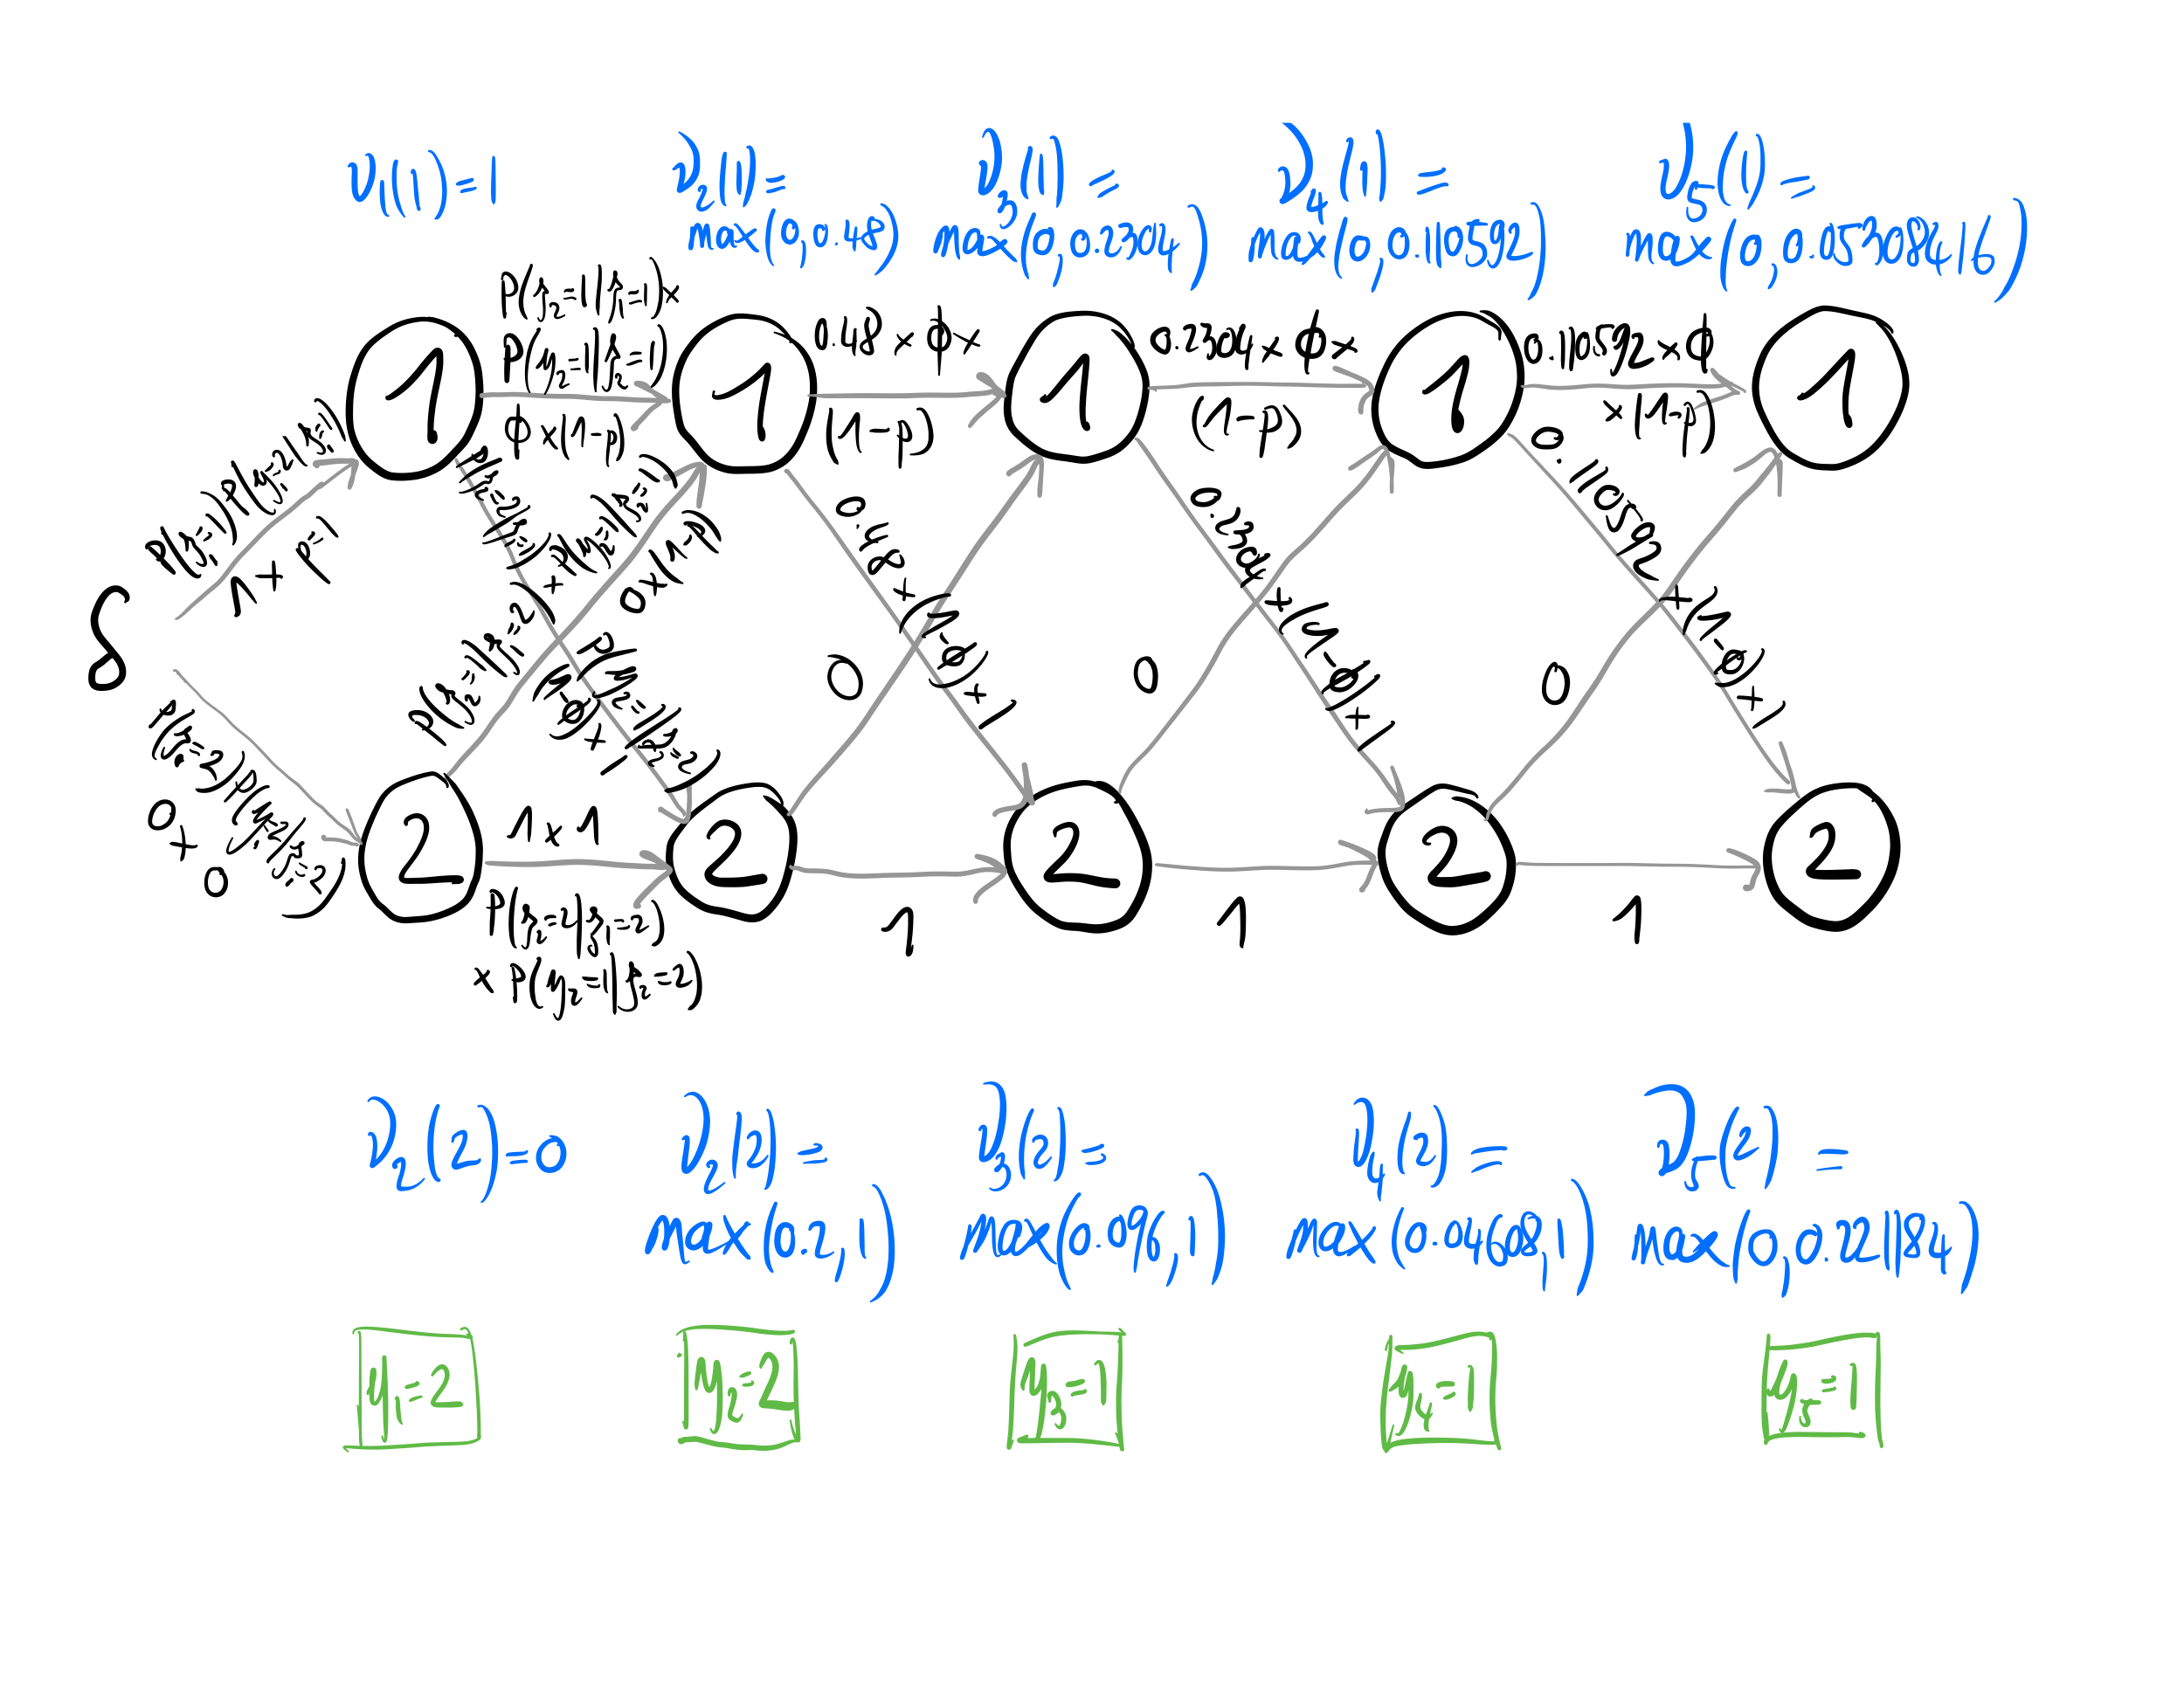
\includegraphics[width=1\linewidth]{images/treillis-viterbi} 

}

\caption{Graphical representation of the Viterbi algorithm with $\phi = 0.8$ and $p = 0.6$. States are alive $z = 1$ or dead $z = 2$ and observations are non-detected $y = 1$ or detected $y = 2$. To be done properly w/ tikz.}\label{fig:treillis-viterbi}
\end{figure}

\hypertarget{implementation}{%
\subsection{Implementation}\label{implementation}}

Let's write a R function to implement the Viterbi algorithm. As parameters, our function will take the transition and observation matrices, the vector of initial state probabilities and the observed sequence of detections and non-detections for which you aim to compute the sequence of states from which it was most likely generated:

\begin{Shaded}
\begin{Highlighting}[]
\CommentTok{\# getViterbi() returns sequence of states that most likely generated sequence of observations}
\CommentTok{\# adapted from https://github.com/vbehnam/viterbi}
\NormalTok{getViterbi }\OtherTok{\textless{}{-}} \ControlFlowTok{function}\NormalTok{(Omega, Gamma, delta, y) \{}
\CommentTok{\# Omega: transition matrix}
\CommentTok{\# Gamma: observation matrix}
\CommentTok{\# delta: vector of initial state probabilities}
\CommentTok{\# y: observed sequence of detections and non{-}detections}
  
\CommentTok{\# get number of states and sampling occasions}
\NormalTok{N }\OtherTok{\textless{}{-}} \FunctionTok{nrow}\NormalTok{(Gamma)}
\NormalTok{T }\OtherTok{\textless{}{-}} \FunctionTok{length}\NormalTok{(y)}
  
\CommentTok{\# nu is the corresponding likelihood}
\NormalTok{nu }\OtherTok{\textless{}{-}} \FunctionTok{matrix}\NormalTok{(}\DecValTok{0}\NormalTok{, }\AttributeTok{nrow =}\NormalTok{ N, }\AttributeTok{ncol =}\NormalTok{ T)}
\CommentTok{\# zz contains the most likely states up until this point}
\NormalTok{zz }\OtherTok{\textless{}{-}} \FunctionTok{matrix}\NormalTok{(}\DecValTok{0}\NormalTok{, }\AttributeTok{nrow =}\NormalTok{ N, }\AttributeTok{ncol =}\NormalTok{ T)}
\NormalTok{firstObs }\OtherTok{\textless{}{-}}\NormalTok{ y[}\DecValTok{1}\NormalTok{]}
  
\CommentTok{\# fill in first columns of both matrices}
\CommentTok{\#nu[,1] \textless{}{-} initial * emission[,firstObs]}
\CommentTok{\#zz[,1] \textless{}{-} 0}
\NormalTok{nu[,}\DecValTok{1}\NormalTok{] }\OtherTok{\textless{}{-}} \FunctionTok{c}\NormalTok{(}\DecValTok{1}\NormalTok{,}\DecValTok{0}\NormalTok{) }\CommentTok{\# initial = (1, 0) * emission[,firstObs] = (1, 0)}
\NormalTok{zz[,}\DecValTok{1}\NormalTok{] }\OtherTok{\textless{}{-}} \DecValTok{1} \CommentTok{\# alive at first occasion}

\ControlFlowTok{for}\NormalTok{ (i }\ControlFlowTok{in} \DecValTok{2}\SpecialCharTok{:}\NormalTok{T) \{}
    \ControlFlowTok{for}\NormalTok{ (j }\ControlFlowTok{in} \DecValTok{1}\SpecialCharTok{:}\NormalTok{N) \{}
\NormalTok{      obs }\OtherTok{\textless{}{-}}\NormalTok{ y[i]}
      \CommentTok{\# initialize to {-}1, then overwritten by for loop coz all possible values are \textgreater{}= 0}
\NormalTok{      nu[j,i] }\OtherTok{\textless{}{-}} \SpecialCharTok{{-}}\DecValTok{1}
      \CommentTok{\# loop to find max and argmax for k}
      \ControlFlowTok{for}\NormalTok{ (k }\ControlFlowTok{in} \DecValTok{1}\SpecialCharTok{:}\NormalTok{N) \{}
\NormalTok{        value }\OtherTok{\textless{}{-}}\NormalTok{ nu[k,i}\DecValTok{{-}1}\NormalTok{] }\SpecialCharTok{*}\NormalTok{ Gamma[k,j] }\SpecialCharTok{*}\NormalTok{ Omega[j,obs]}
        \ControlFlowTok{if}\NormalTok{ (value }\SpecialCharTok{\textgreater{}}\NormalTok{ nu[j,i]) \{}
          \CommentTok{\# maximizing for k}
\NormalTok{          nu[j,i] }\OtherTok{\textless{}{-}}\NormalTok{ value}
          \CommentTok{\# argmaximizing for k}
\NormalTok{          zz[j,i] }\OtherTok{\textless{}{-}}\NormalTok{ k}
\NormalTok{        \}}
\NormalTok{      \}}
\NormalTok{    \}}
\NormalTok{  \}}
  \CommentTok{\# mlp = most likely path}
\NormalTok{  mlp }\OtherTok{\textless{}{-}} \FunctionTok{numeric}\NormalTok{(T)}
  \CommentTok{\# argmax for stateSeq[,T]}
\NormalTok{  am }\OtherTok{\textless{}{-}} \FunctionTok{which.max}\NormalTok{(nu[,T])}
\NormalTok{  mlp[T] }\OtherTok{\textless{}{-}}\NormalTok{ zz[am,T]}
  
  \CommentTok{\# backtrace using backpointers}
  \ControlFlowTok{for}\NormalTok{ (i }\ControlFlowTok{in}\NormalTok{ T}\SpecialCharTok{:}\DecValTok{2}\NormalTok{) \{}
\NormalTok{    zm }\OtherTok{\textless{}{-}} \FunctionTok{which.max}\NormalTok{(nu[,i])}
\NormalTok{    mlp[i}\DecValTok{{-}1}\NormalTok{] }\OtherTok{\textless{}{-}}\NormalTok{ zz[zm,i]}
\NormalTok{  \}}
  \FunctionTok{return}\NormalTok{(mlp)}
\NormalTok{\}}
\end{Highlighting}
\end{Shaded}

Note that instead of writing your own R function, you could use a built-in function from an existing R package to implement the Viterbi algorithm\footnote{For example, the \texttt{viterbi()} function from the HMM and depmixS4 packages.}, and call it from NIMBLE as we have seen in Section \ref{callrfninnimble}. The difficulty is that HMM for capture-recapture data have specific features that make standard functions not adapted and requires coding your own Viterbi function. In particular, we have to deal with detection at first encounter, which is not estimated but is always one because an individual has to be captured to be marked and released for the first time. Also, our transition and observation matrices are not always homogeneous and may depend on time.

Let's test our \texttt{getViterbi()} function with our previous example. Remember animal \#15 has the encounter history (2, 1, 1, 1, 1) which was generated from the sequence of states (1, 1, 2, 2, 2). Applying our function to that animal encounter history, we get:

\begin{Shaded}
\begin{Highlighting}[]
\NormalTok{delta }\CommentTok{\# Vector of initial states probabilities}
\DocumentationTok{\#\# [1] 1 0}
\NormalTok{Gamma }\CommentTok{\# Transition matrix}
\DocumentationTok{\#\#      [,1] [,2]}
\DocumentationTok{\#\# [1,]  0.8  0.2}
\DocumentationTok{\#\# [2,]  0.0  1.0}
\NormalTok{Omega }\CommentTok{\# Observation matrix}
\DocumentationTok{\#\#      [,1] [,2]}
\DocumentationTok{\#\# [1,]  0.4  0.6}
\DocumentationTok{\#\# [2,]  1.0  0.0}
\FunctionTok{getViterbi}\NormalTok{(}\AttributeTok{Omega =}\NormalTok{ Omega, }
           \AttributeTok{Gamma =}\NormalTok{ Gamma, }
           \AttributeTok{delta =}\NormalTok{ delta, }
           \AttributeTok{y =}\NormalTok{ y[}\DecValTok{15}\NormalTok{,] }\SpecialCharTok{+} \DecValTok{1}\NormalTok{)}
\DocumentationTok{\#\# [1] 1 2 2 2 2}
\end{Highlighting}
\end{Shaded}

The Viterbi algorithm does pretty well at recovering the latent states, despite incorrectly decoding a death in the second winter while individual \#15 only dies in the third winter. We obtained the same results by implementing the Viterbi algorithm by hand in Section \ref{viterbi-theory}.

Now that we have a function that implements the Viterbi algorithm, we can use it with our MCMC outputs. You have two options, either you apply Viterbi to each MCMC iteration then you compute the posterior median or mode path for each individual, or you compute the posterior mean or median of the transition and observation matrices then you apply Viterbi to each individual encounter history.

For both options, we will need the values from the posterior distributions of survival and detection probabilities:

\begin{Shaded}
\begin{Highlighting}[]
\NormalTok{phi }\OtherTok{\textless{}{-}} \FunctionTok{c}\NormalTok{(mcmc.output}\SpecialCharTok{$}\NormalTok{chain1[,}\StringTok{\textquotesingle{}phi\textquotesingle{}}\NormalTok{], mcmc.output}\SpecialCharTok{$}\NormalTok{chain2[,}\StringTok{\textquotesingle{}phi\textquotesingle{}}\NormalTok{])}
\NormalTok{p }\OtherTok{\textless{}{-}} \FunctionTok{c}\NormalTok{(mcmc.output}\SpecialCharTok{$}\NormalTok{chain1[,}\StringTok{\textquotesingle{}p\textquotesingle{}}\NormalTok{], mcmc.output}\SpecialCharTok{$}\NormalTok{chain2[,}\StringTok{\textquotesingle{}p\textquotesingle{}}\NormalTok{])}
\end{Highlighting}
\end{Shaded}

\hypertarget{compute-average}{%
\subsection{Compute first, average after}\label{compute-average}}

First option is to apply Viterbi to each MCMC sample, then to compute median of the MCMC Viterbi paths for each observed sequence:

\begin{Shaded}
\begin{Highlighting}[]
\NormalTok{niter }\OtherTok{\textless{}{-}} \FunctionTok{length}\NormalTok{(p)}
\NormalTok{T }\OtherTok{\textless{}{-}} \DecValTok{5}
\NormalTok{res }\OtherTok{\textless{}{-}} \FunctionTok{matrix}\NormalTok{(}\ConstantTok{NA}\NormalTok{, }\AttributeTok{nrow =} \FunctionTok{nrow}\NormalTok{(y), }\AttributeTok{ncol =}\NormalTok{ T)}
\ControlFlowTok{for}\NormalTok{ (i }\ControlFlowTok{in} \DecValTok{1}\SpecialCharTok{:}\FunctionTok{nrow}\NormalTok{(y))\{}
\NormalTok{  res\_mcmc }\OtherTok{\textless{}{-}} \FunctionTok{matrix}\NormalTok{(}\ConstantTok{NA}\NormalTok{, }\AttributeTok{nrow =}\NormalTok{ niter, }\AttributeTok{ncol =}\NormalTok{ T)}
  \ControlFlowTok{for}\NormalTok{ (j }\ControlFlowTok{in} \DecValTok{1}\SpecialCharTok{:}\NormalTok{niter)\{}
    \CommentTok{\# Initial states}
\NormalTok{    delta }\OtherTok{\textless{}{-}} \FunctionTok{c}\NormalTok{(}\DecValTok{1}\NormalTok{, }\DecValTok{0}\NormalTok{)}
    \CommentTok{\# Transition matrix}
\NormalTok{    transition }\OtherTok{\textless{}{-}} \FunctionTok{matrix}\NormalTok{(}\ConstantTok{NA}\NormalTok{, }\DecValTok{2}\NormalTok{, }\DecValTok{2}\NormalTok{)}
\NormalTok{    transition[}\DecValTok{1}\NormalTok{,}\DecValTok{1}\NormalTok{] }\OtherTok{\textless{}{-}}\NormalTok{ phi[j]      }\CommentTok{\# Pr(alive t {-}\textgreater{} alive t+1)}
\NormalTok{    transition[}\DecValTok{1}\NormalTok{,}\DecValTok{2}\NormalTok{] }\OtherTok{\textless{}{-}} \DecValTok{1} \SpecialCharTok{{-}}\NormalTok{ phi[j]  }\CommentTok{\# Pr(alive t {-}\textgreater{} dead t+1)}
\NormalTok{    transition[}\DecValTok{2}\NormalTok{,}\DecValTok{1}\NormalTok{] }\OtherTok{\textless{}{-}} \DecValTok{0}        \CommentTok{\# Pr(dead t {-}\textgreater{} alive t+1)}
\NormalTok{    transition[}\DecValTok{2}\NormalTok{,}\DecValTok{2}\NormalTok{] }\OtherTok{\textless{}{-}} \DecValTok{1}        \CommentTok{\# Pr(dead t {-}\textgreater{} dead t+1)}
    \CommentTok{\# Observation matrix }
\NormalTok{    emission }\OtherTok{\textless{}{-}} \FunctionTok{matrix}\NormalTok{(}\ConstantTok{NA}\NormalTok{, }\DecValTok{2}\NormalTok{, }\DecValTok{2}\NormalTok{)}
\NormalTok{    emission[}\DecValTok{1}\NormalTok{,}\DecValTok{1}\NormalTok{] }\OtherTok{\textless{}{-}} \DecValTok{1} \SpecialCharTok{{-}}\NormalTok{ p[j]      }\CommentTok{\# Pr(alive t {-}\textgreater{} non{-}detected t)}
\NormalTok{    emission[}\DecValTok{1}\NormalTok{,}\DecValTok{2}\NormalTok{] }\OtherTok{\textless{}{-}}\NormalTok{ p[j]          }\CommentTok{\# Pr(alive t {-}\textgreater{} detected t)}
\NormalTok{    emission[}\DecValTok{2}\NormalTok{,}\DecValTok{1}\NormalTok{] }\OtherTok{\textless{}{-}} \DecValTok{1}          \CommentTok{\# Pr(dead t {-}\textgreater{} non{-}detected t)}
\NormalTok{    emission[}\DecValTok{2}\NormalTok{,}\DecValTok{2}\NormalTok{] }\OtherTok{\textless{}{-}} \DecValTok{0}          \CommentTok{\# Pr(dead t {-}\textgreater{} detected t)}
\NormalTok{    res\_mcmc[j,}\DecValTok{1}\SpecialCharTok{:}\NormalTok{T] }\OtherTok{\textless{}{-}} \FunctionTok{getViterbi}\NormalTok{(emission, transition, delta, y[i,] }\SpecialCharTok{+} \DecValTok{1}\NormalTok{)}
\NormalTok{  \}}
\NormalTok{  res[i, }\DecValTok{1}\SpecialCharTok{:}\FunctionTok{length}\NormalTok{(y[}\DecValTok{1}\NormalTok{,])] }\OtherTok{\textless{}{-}} \FunctionTok{apply}\NormalTok{(res\_mcmc, }\DecValTok{2}\NormalTok{, median)}
\NormalTok{\}}
\end{Highlighting}
\end{Shaded}

You can compare the Viterbi decoding to the actual states \(z\):
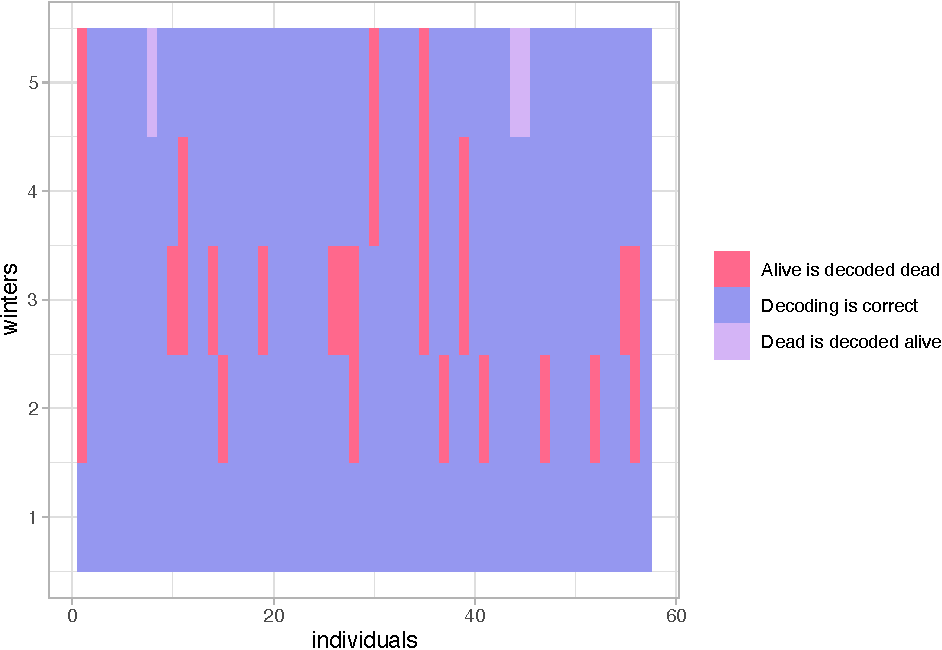
\includegraphics{banana-book_files/figure-latex/viterbiaveragecompute-1.pdf}

Decoding is correct except that the alive actual state is often decoded as the dead state by the Viterbi algorithm. Note that here we compute the Viterbi paths after we run NIMBLE. You could turn the R function \texttt{getViterbi()} into a NIMBLE function and plug it in your model code to apply Viterbi. This would not make any difference except perhaps to increase MCMC computation times.

\hypertarget{average-first-compute-after}{%
\subsection{Average first, compute after}\label{average-first-compute-after}}

Second option is to compute the posterior mean of the observation and transition matrices, then to apply Viterbi:

\begin{Shaded}
\begin{Highlighting}[]
\CommentTok{\# Initial states}
\NormalTok{delta }\OtherTok{\textless{}{-}} \FunctionTok{c}\NormalTok{(}\DecValTok{1}\NormalTok{, }\DecValTok{0}\NormalTok{)}
\CommentTok{\# Transition matrix}
\NormalTok{transition }\OtherTok{\textless{}{-}} \FunctionTok{matrix}\NormalTok{(}\ConstantTok{NA}\NormalTok{, }\DecValTok{2}\NormalTok{, }\DecValTok{2}\NormalTok{)}
\NormalTok{transition[}\DecValTok{1}\NormalTok{,}\DecValTok{1}\NormalTok{] }\OtherTok{\textless{}{-}} \FunctionTok{mean}\NormalTok{(phi)      }\CommentTok{\# Pr(alive t {-}\textgreater{} alive t+1)}
\NormalTok{transition[}\DecValTok{1}\NormalTok{,}\DecValTok{2}\NormalTok{] }\OtherTok{\textless{}{-}} \DecValTok{1} \SpecialCharTok{{-}} \FunctionTok{mean}\NormalTok{(phi)  }\CommentTok{\# Pr(alive t {-}\textgreater{} dead t+1)}
\NormalTok{transition[}\DecValTok{2}\NormalTok{,}\DecValTok{1}\NormalTok{] }\OtherTok{\textless{}{-}} \DecValTok{0}              \CommentTok{\# Pr(dead t {-}\textgreater{} alive t+1)}
\NormalTok{transition[}\DecValTok{2}\NormalTok{,}\DecValTok{2}\NormalTok{] }\OtherTok{\textless{}{-}} \DecValTok{1}              \CommentTok{\# Pr(dead t {-}\textgreater{} dead t+1)}
\CommentTok{\# Observation matrix }
\NormalTok{emission }\OtherTok{\textless{}{-}} \FunctionTok{matrix}\NormalTok{(}\ConstantTok{NA}\NormalTok{, }\DecValTok{2}\NormalTok{, }\DecValTok{2}\NormalTok{)}
\NormalTok{emission[}\DecValTok{1}\NormalTok{,}\DecValTok{1}\NormalTok{] }\OtherTok{\textless{}{-}} \DecValTok{1} \SpecialCharTok{{-}} \FunctionTok{mean}\NormalTok{(p)      }\CommentTok{\# Pr(alive t {-}\textgreater{} non{-}detected t)}
\NormalTok{emission[}\DecValTok{1}\NormalTok{,}\DecValTok{2}\NormalTok{] }\OtherTok{\textless{}{-}} \FunctionTok{mean}\NormalTok{(p)          }\CommentTok{\# Pr(alive t {-}\textgreater{} detected t)}
\NormalTok{emission[}\DecValTok{2}\NormalTok{,}\DecValTok{1}\NormalTok{] }\OtherTok{\textless{}{-}} \DecValTok{1}                \CommentTok{\# Pr(dead t {-}\textgreater{} non{-}detected t)}
\NormalTok{emission[}\DecValTok{2}\NormalTok{,}\DecValTok{2}\NormalTok{] }\OtherTok{\textless{}{-}} \DecValTok{0}                \CommentTok{\# Pr(dead t {-}\textgreater{} detected t)}
\NormalTok{res }\OtherTok{\textless{}{-}} \FunctionTok{matrix}\NormalTok{(}\ConstantTok{NA}\NormalTok{, }\AttributeTok{nrow =} \FunctionTok{nrow}\NormalTok{(y), }\AttributeTok{ncol =}\NormalTok{ T)}
\ControlFlowTok{for}\NormalTok{ (i }\ControlFlowTok{in} \DecValTok{1}\SpecialCharTok{:}\FunctionTok{nrow}\NormalTok{(y))\{}
\NormalTok{  res[i, }\DecValTok{1}\SpecialCharTok{:}\FunctionTok{length}\NormalTok{(y[}\DecValTok{1}\NormalTok{,]) ] }\OtherTok{\textless{}{-}} \FunctionTok{getViterbi}\NormalTok{(emission, transition, delta, y[i,] }\SpecialCharTok{+} \DecValTok{1}\NormalTok{)}
\NormalTok{\}}
\end{Highlighting}
\end{Shaded}

Again, you can compare the result of the Viterbi decoding to the actual states we simulated and used to generate the observations:
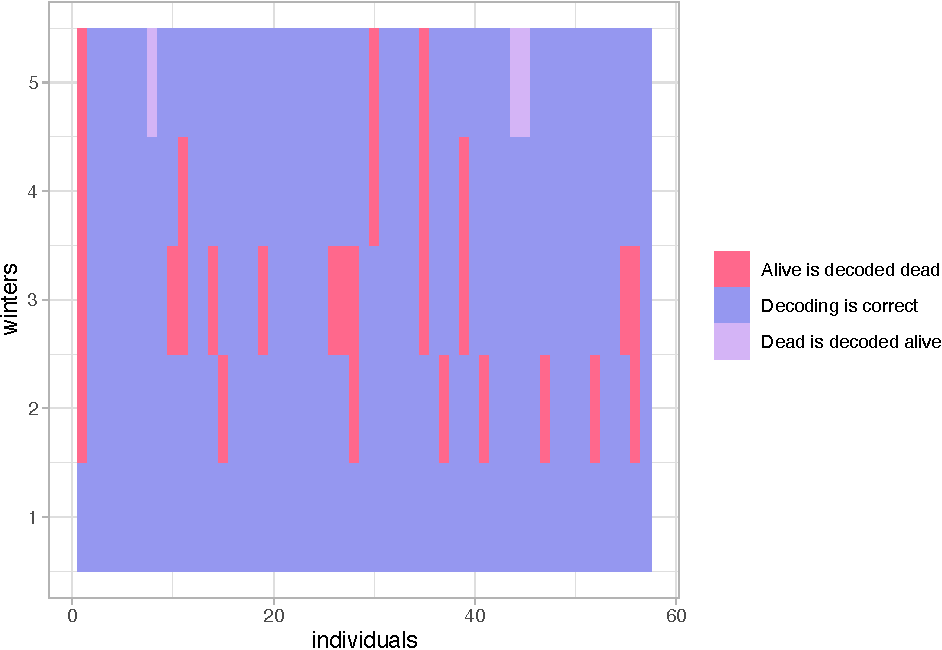
\includegraphics{banana-book_files/figure-latex/viterbicomputeaverage-1.pdf}

The results are very similar to those we obtained in Section \ref{compute-average}, and Figure \ref{fig:viterbicomputeaverage} is indisguishable from Figure \ref{fig:viterbiaveragecompute}.

\hypertarget{summary-2}{%
\section{Summary}\label{summary-2}}

\begin{itemize}
\item
  A HMM is a model that consists of two parts: i) an unobserved sequence of discrete random variables - the states - satisfying the Markovian property (future states depends on current states only and not on past states) and ii) an observed sequence of discrete random variables - the observations - depending only on the current state.
\item
  The Bayesian approach together with MCMC simulations allow estimating survival and detection probabilities as well as individual latent states alive or dead with the complete likelihood. If you can afford the computation times, then using the complete likelihood is the easiest path for model fitting.
\item
  If you do not need to infer the latent states, you can use the marginal likelihood via the forward algorithm. By avoiding to sample the latent states, you usually get better mixing and faster convergence.
\item
  If you do need to infer the latent states, and you cannot afford the computation times of the complete likelihood, then you can go for the marginal likelihood in conjunction with the Viterbi algorithm to decode the latent states.
\item
  If the computational burden is still an issue, and you have individuals that share the same encounter history, you can use a pooled likelihood to speed up the marginal likelihood evaluation and MCMC convergence.
\end{itemize}

\hypertarget{suggested-reading-2}{%
\section{Suggested reading}\label{suggested-reading-2}}

\begin{itemize}
\item
  Jurafsky D. and Martin J.H. (2021) \href{https://web.stanford.edu/~jurafsky/slp3/A.pdf}{Hidden Markov models}. In Speech and Language Processing. 3rd edition. Pearson Education UK, 2021.
\item
  McClintock B.T., Langrock R., Gimenez O., Cam E., Borchers D.L., Glennie R. and Patterson T.A. (2020), \href{https://onlinelibrary.wiley.com/doi/full/10.1111/ele.13610}{Uncovering ecological state dynamics with hidden Markov models}. Ecology Letters, 23: 1878-1903.
\item
  Rabiner L.R. (1989). \href{https://web.ece.ucsb.edu/Faculty/Rabiner/ece259/Reprints/tutorial\%20on\%20hmm\%20and\%20applications.pdf}{A tutorial on hidden Markov models and selected applications in speech recognition}. Proceedings of the IEEE, 77:257-286.
\end{itemize}

\begin{itemize}
\tightlist
\item
  Zucchini W., MacDonald I.L. and Langrock R. (2016) \href{https://www.routledge.com/Hidden-Markov-Models-for-Time-Series-An-Introduction-Using-R-Second-Edition/Zucchini-MacDonald-Langrock/p/book/9781482253832}{Hidden Markov Models for Time Series: An Introduction Using R (2nd ed)}. Chapman and Hall/CRC.
\end{itemize}

\hypertarget{part-ii.-transitions}{%
\part{II. Transitions}\label{part-ii.-transitions}}

\hypertarget{introduction-4}{%
\chapter*{Introduction}\label{introduction-4}}


\hypertarget{survival}{%
\chapter{Survival}\label{survival}}

WORK IN PROGRESS.

\hypertarget{introduction-5}{%
\section{Introduction}\label{introduction-5}}

Blabla. Blabla. Need to explain sensitivity analyses somewhere.

\begin{Shaded}
\begin{Highlighting}[]
\NormalTok{knitr}\SpecialCharTok{::}\FunctionTok{include\_graphics}\NormalTok{(}\StringTok{"images/lebreton.png"}\NormalTok{)}
\end{Highlighting}
\end{Shaded}


\includegraphics[width=13.12in]{images/lebreton}

\hypertarget{history-of-the-cormack-jolly-seber-cjs-model}{%
\section{History of the Cormack-Jolly-Seber (CJS) model}\label{history-of-the-cormack-jolly-seber-cjs-model}}

S.T. Buckland (2016). A Conversation with Richard M. Cormack. Statistical Science 31: 142-150.

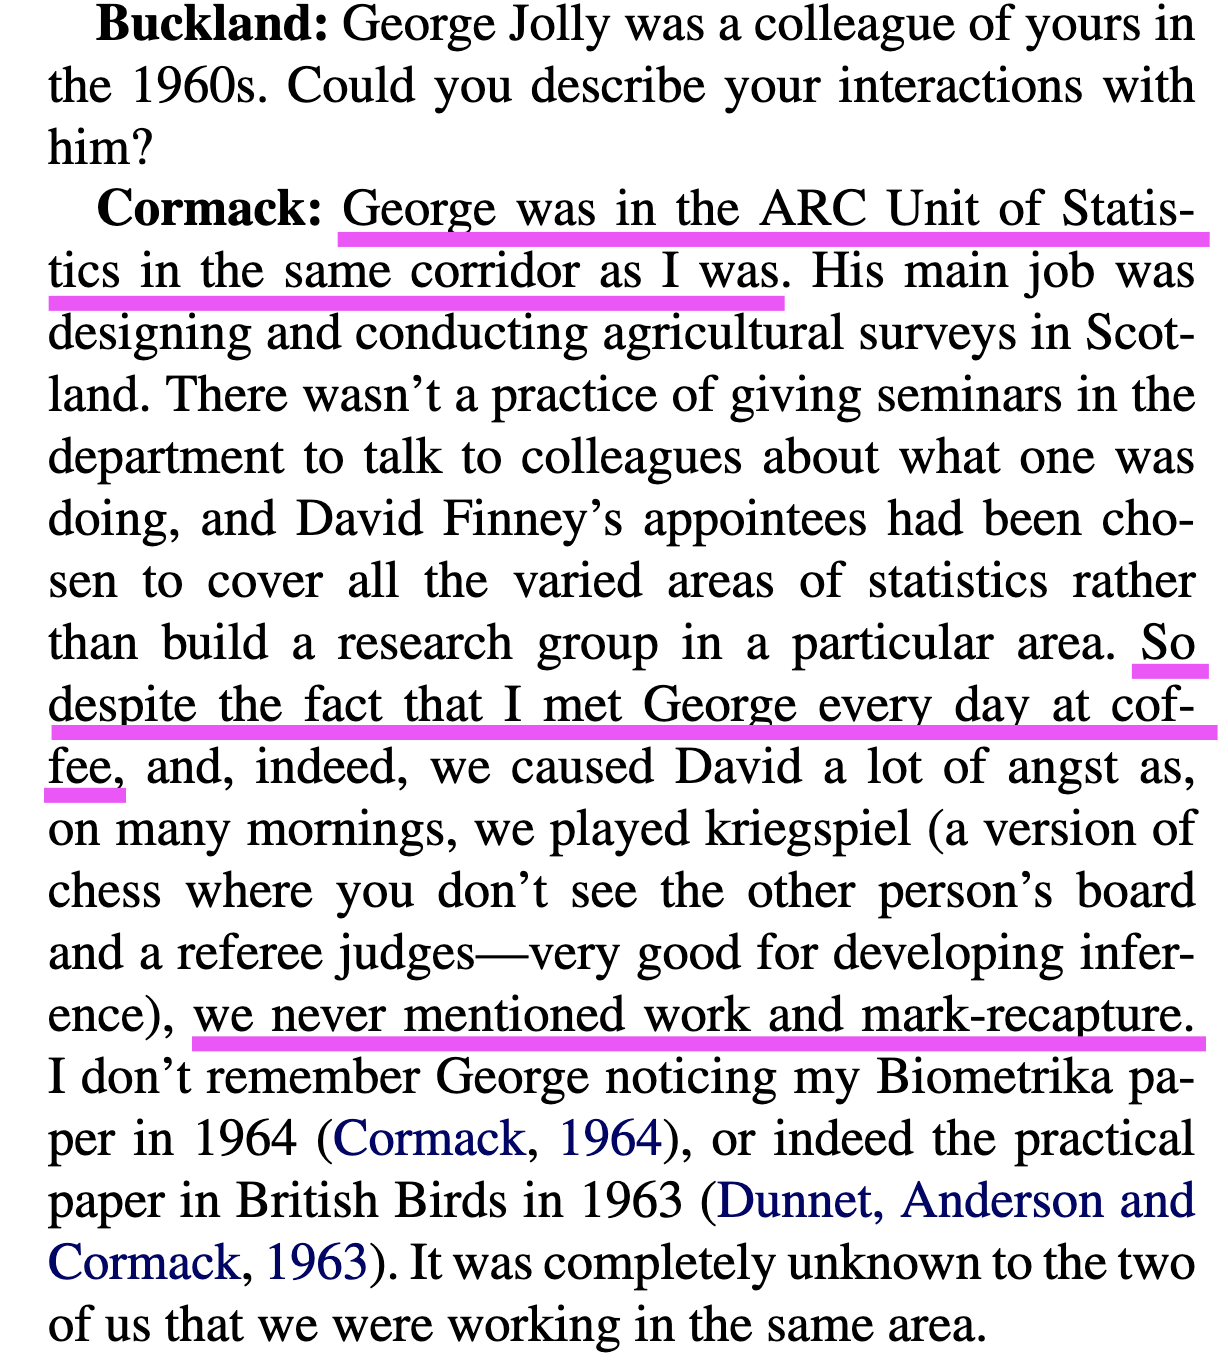
\includegraphics[width=0.8\linewidth]{images/cormack-left}

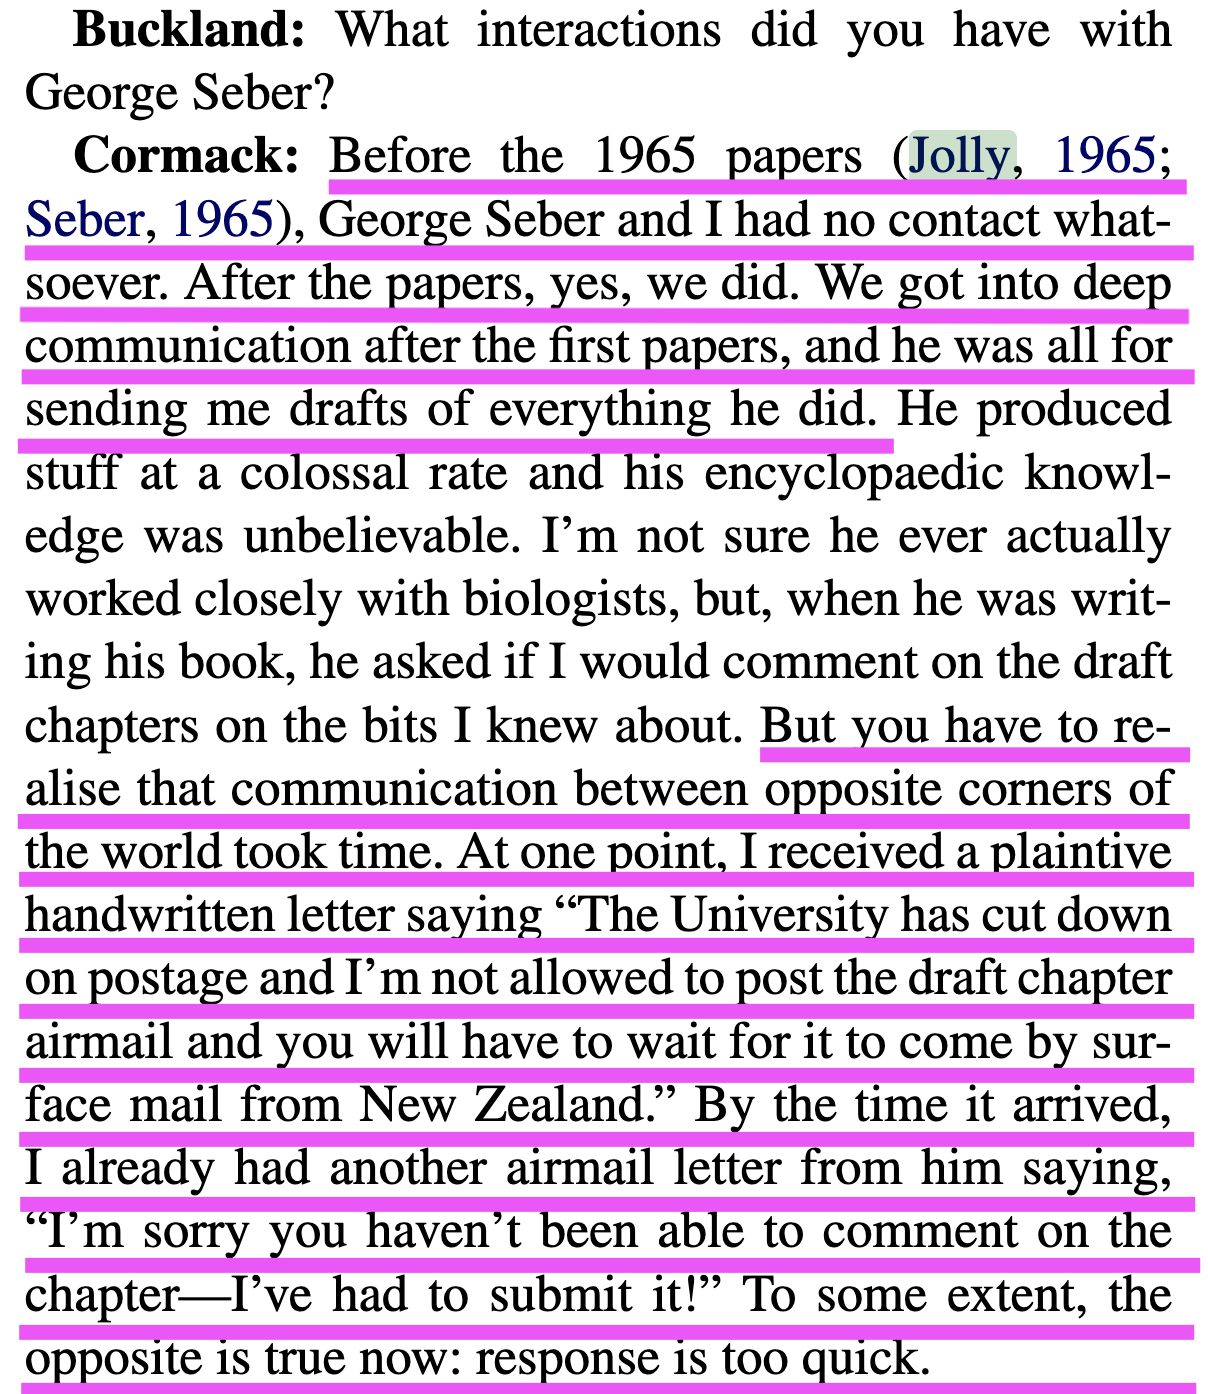
\includegraphics[width=0.8\linewidth]{images/cormack-right}

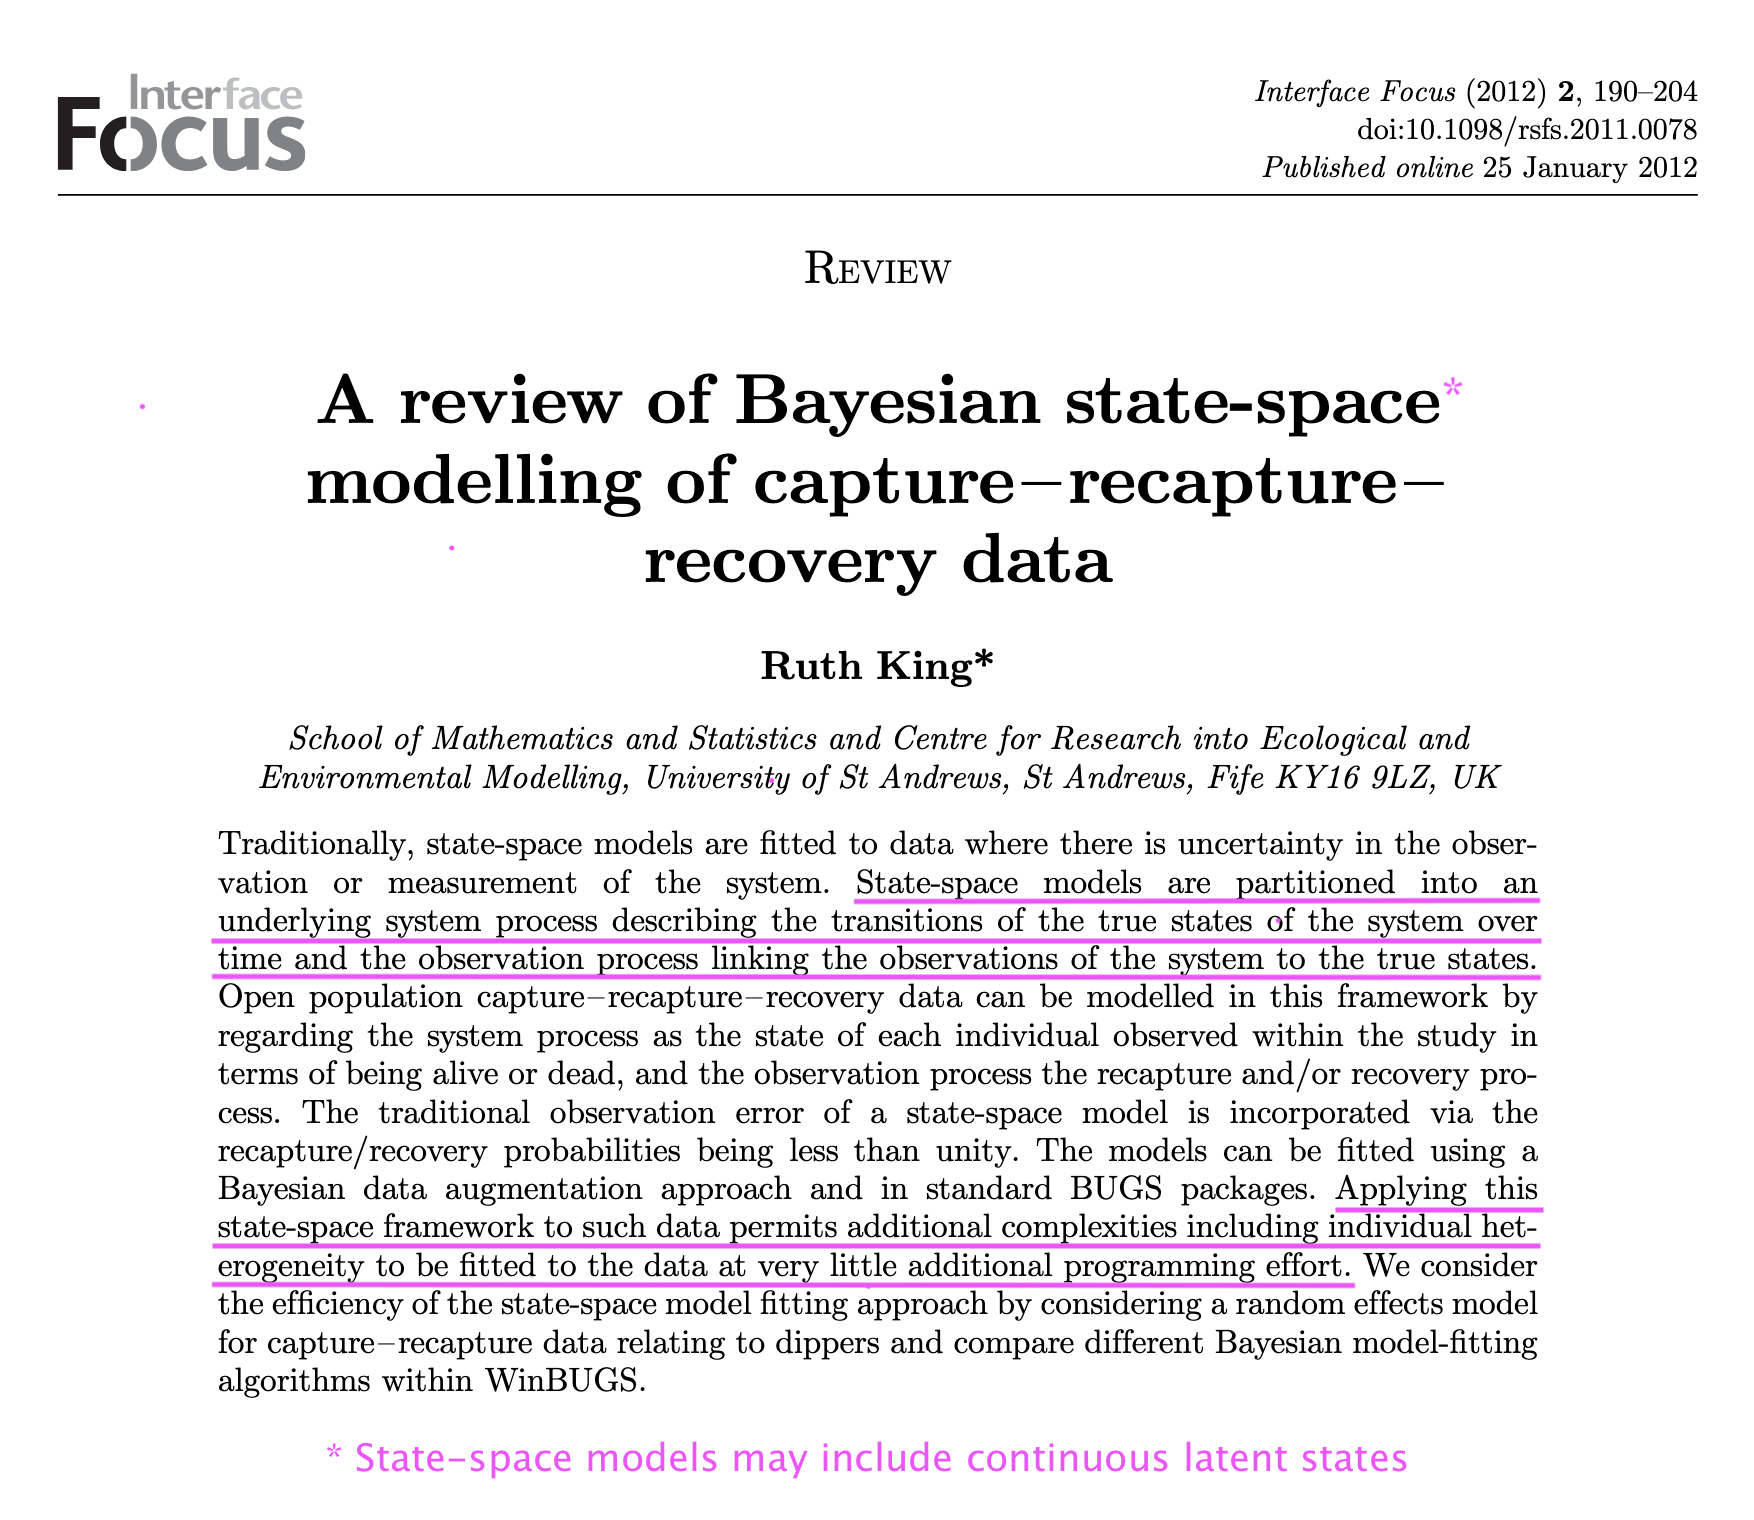
\includegraphics[width=0.7\linewidth]{images/king}

Bayesian uptake

\hypertarget{what-weve-seen-so-far}{%
\section{What we've seen so far}\label{what-weve-seen-so-far}}

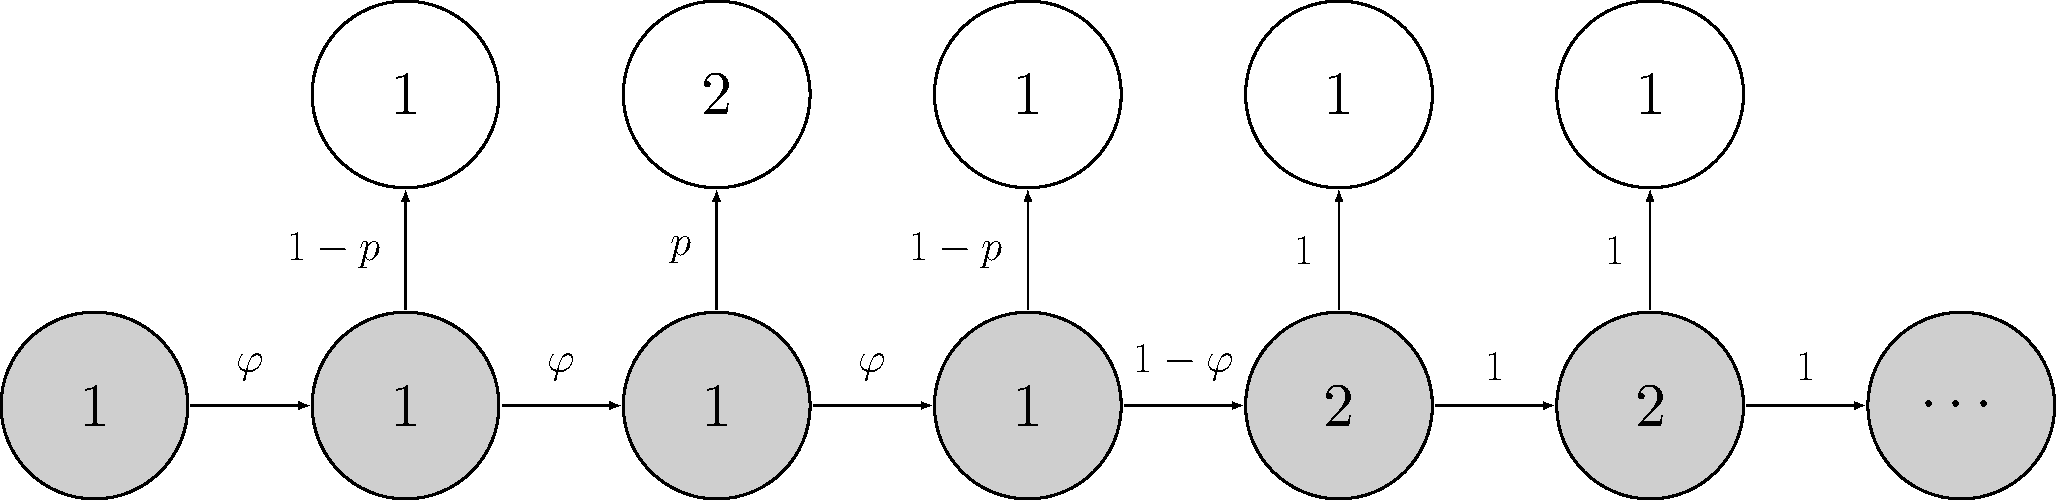
\includegraphics{banana-book_files/figure-latex/unnamed-chunk-173-1.pdf}

For states (in gray), \(z = 1\) is alive, \(z = 2\) is dead.

For observations (in white), \(y = 1\) is non-detected, \(y = 2\) is detected

\hypertarget{in-the-cjs-model-survival-and-recapture-are-time-varying}{%
\section{In the CJS model, survival and recapture are time-varying}\label{in-the-cjs-model-survival-and-recapture-are-time-varying}}

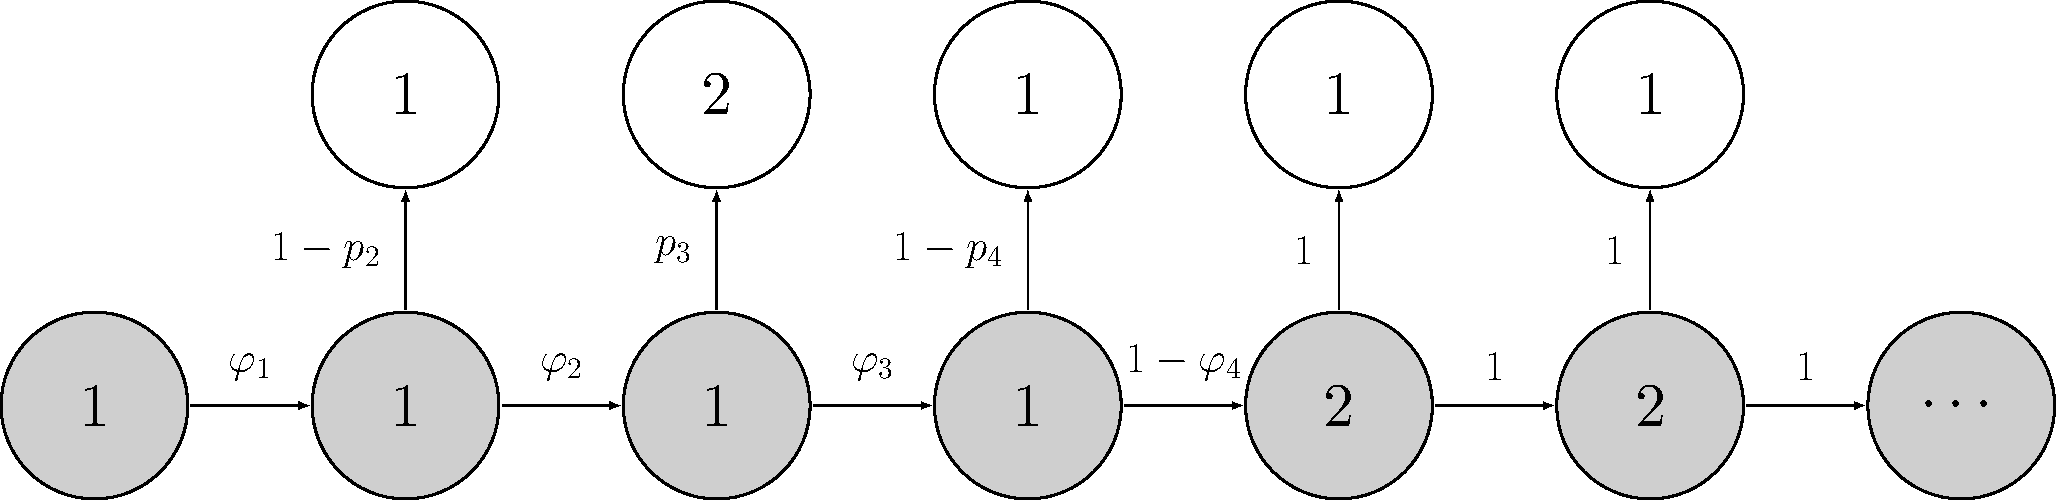
\includegraphics{banana-book_files/figure-latex/unnamed-chunk-174-1.pdf}

Survival probability is \(\phi_t = \Pr(z_{t+1} = 1 | z_t = 1)\).

Recapture (detection) probability is \(p_t = \Pr(y_{t} = 1 | z_t = 1)\).

Accounts for variation in e.g.~environmental conditions (survival) or sampling effort (detection).

\hypertarget{capture-mark-and-recapture}{%
\section{Capture, mark and recapture}\label{capture-mark-and-recapture}}

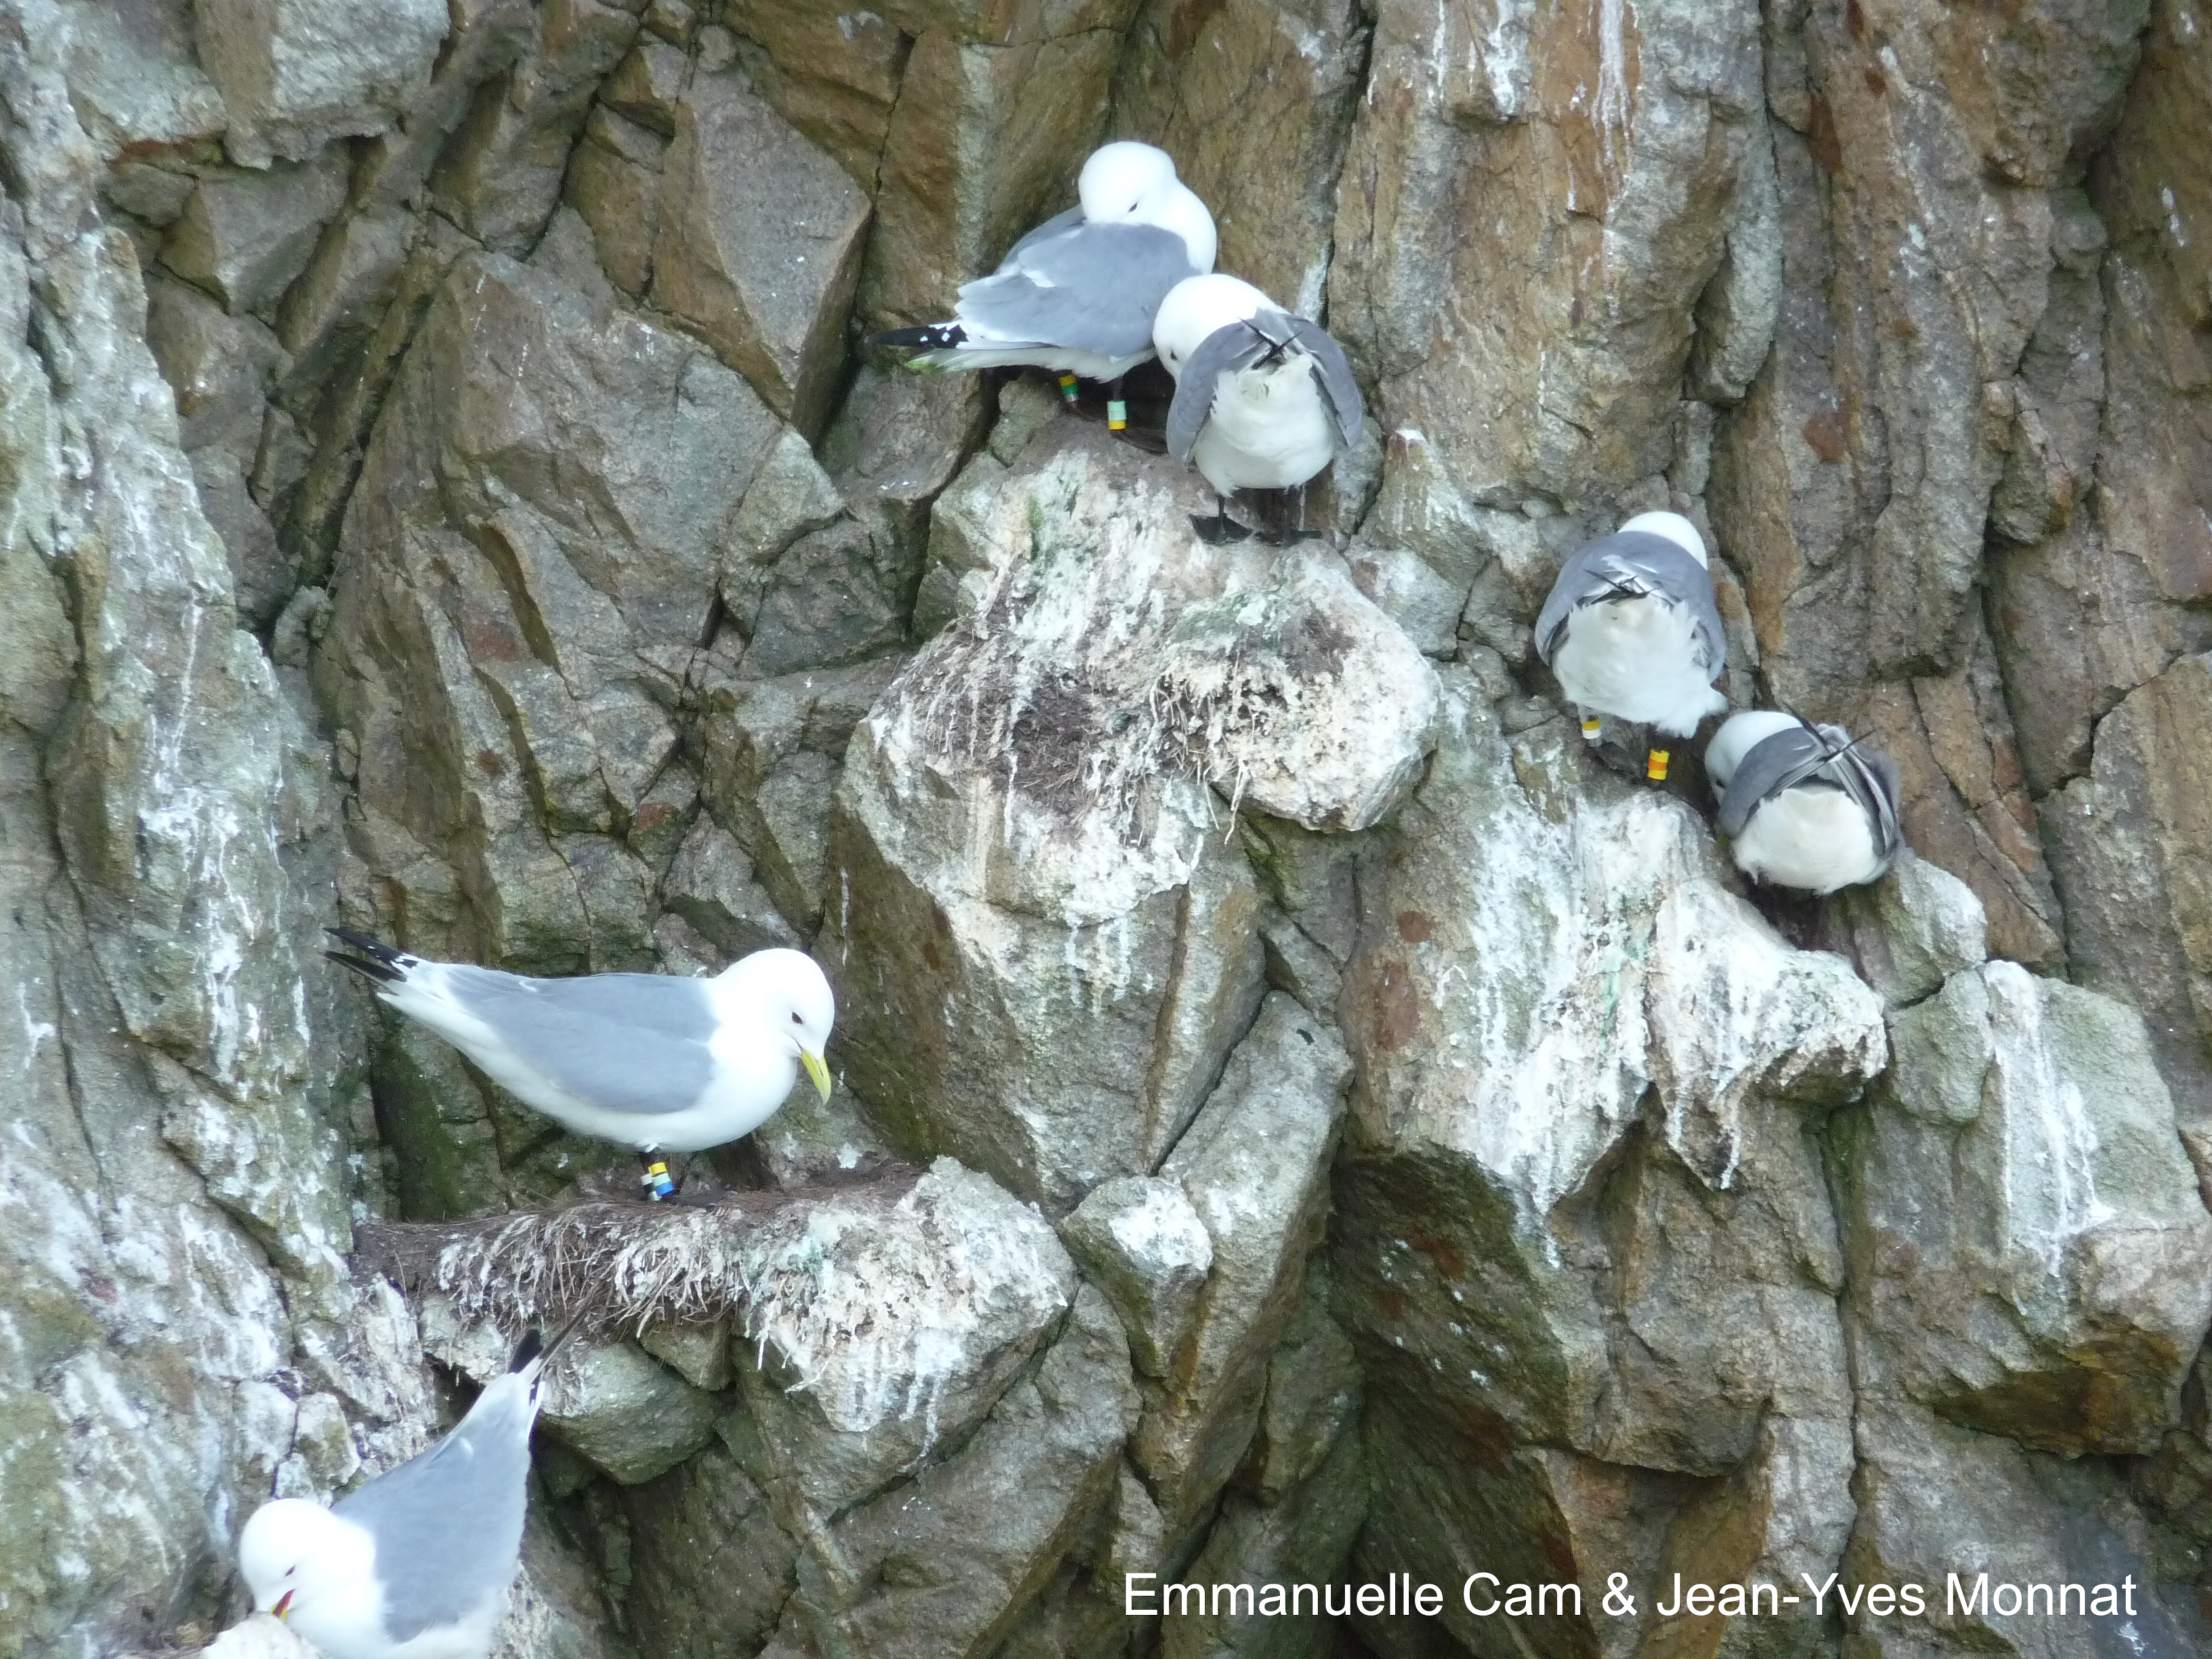
\includegraphics[width=0.9\linewidth]{images/gull}

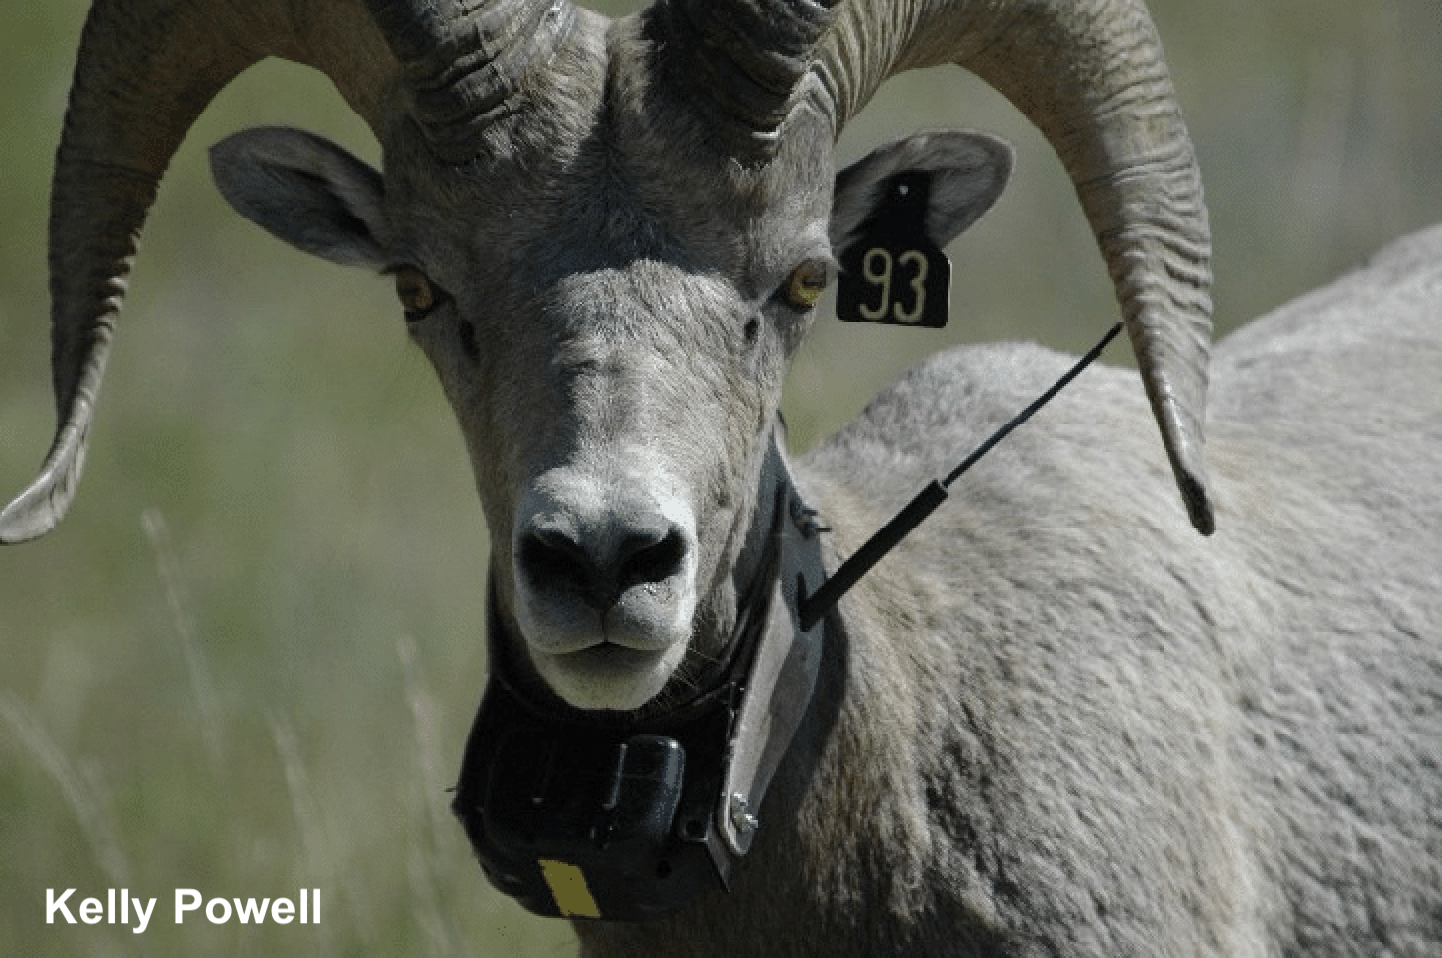
\includegraphics[width=1.1\linewidth]{images/bighorn}

Artificial marks

\hypertarget{capture-mark-and-recapture-1}{%
\section{Capture, mark and recapture}\label{capture-mark-and-recapture-1}}

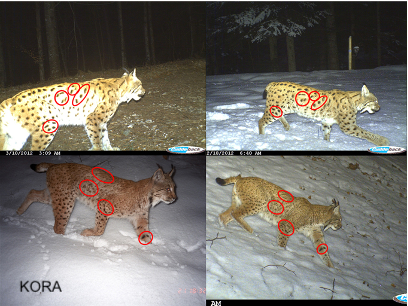
\includegraphics[width=0.9\linewidth]{images/lynx}

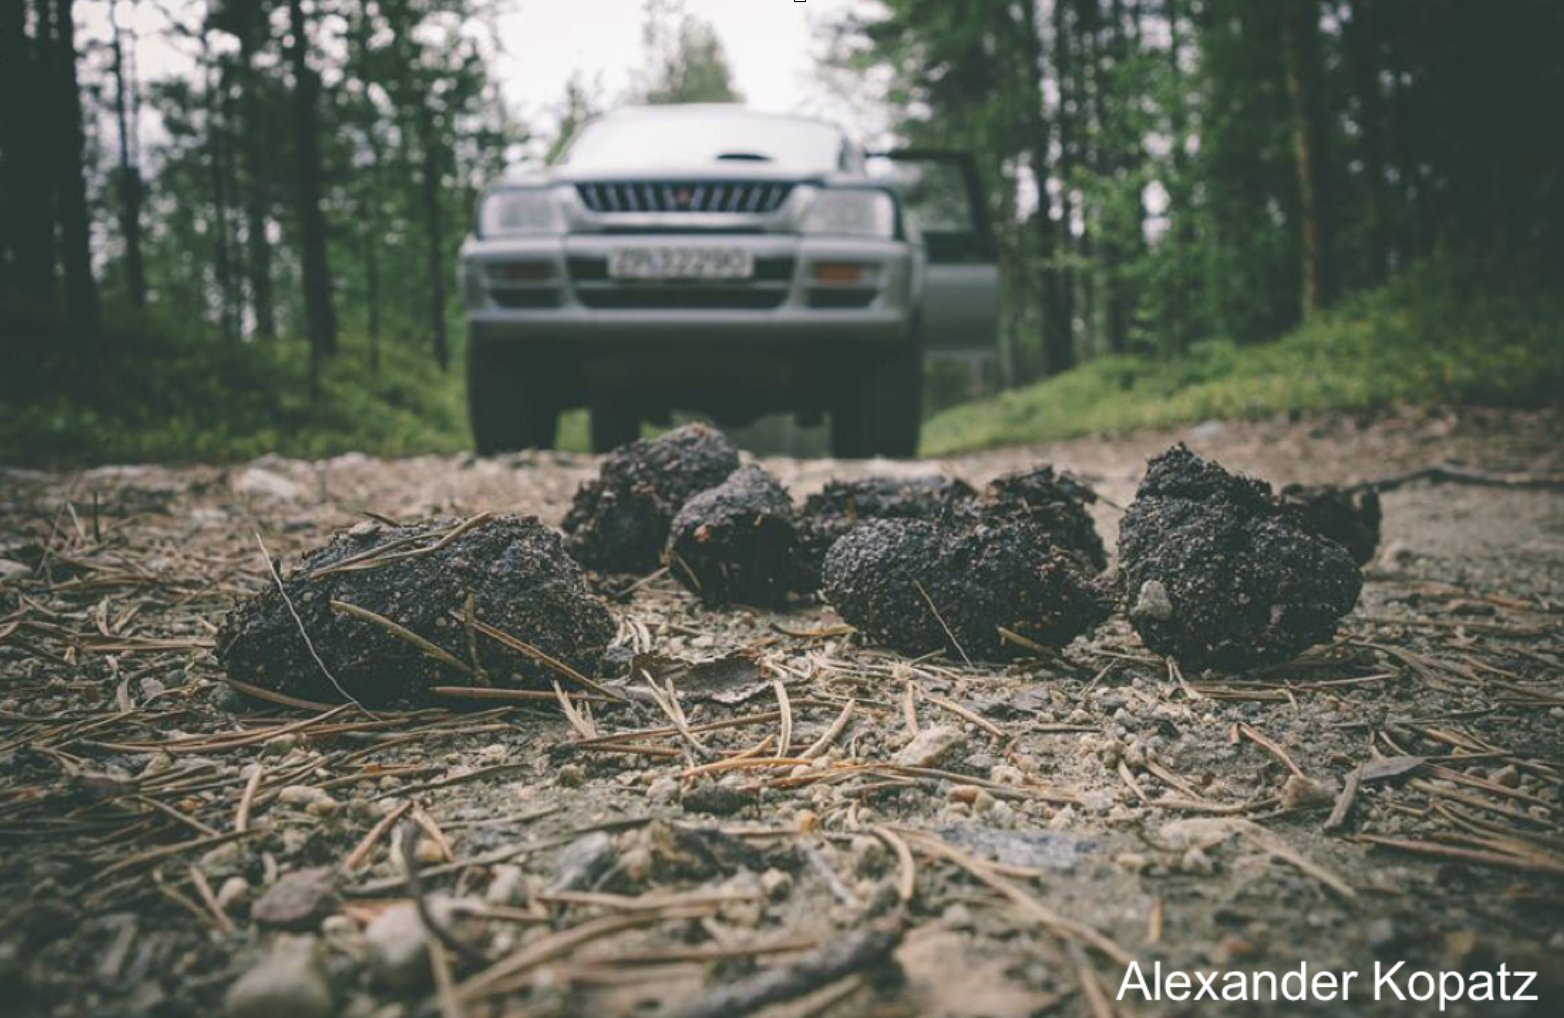
\includegraphics[width=1.2\linewidth]{images/bearscat}

Natural marks

\hypertarget{the-famous-dipper-example}{%
\section{The famous Dipper example}\label{the-famous-dipper-example}}

\begin{figure}
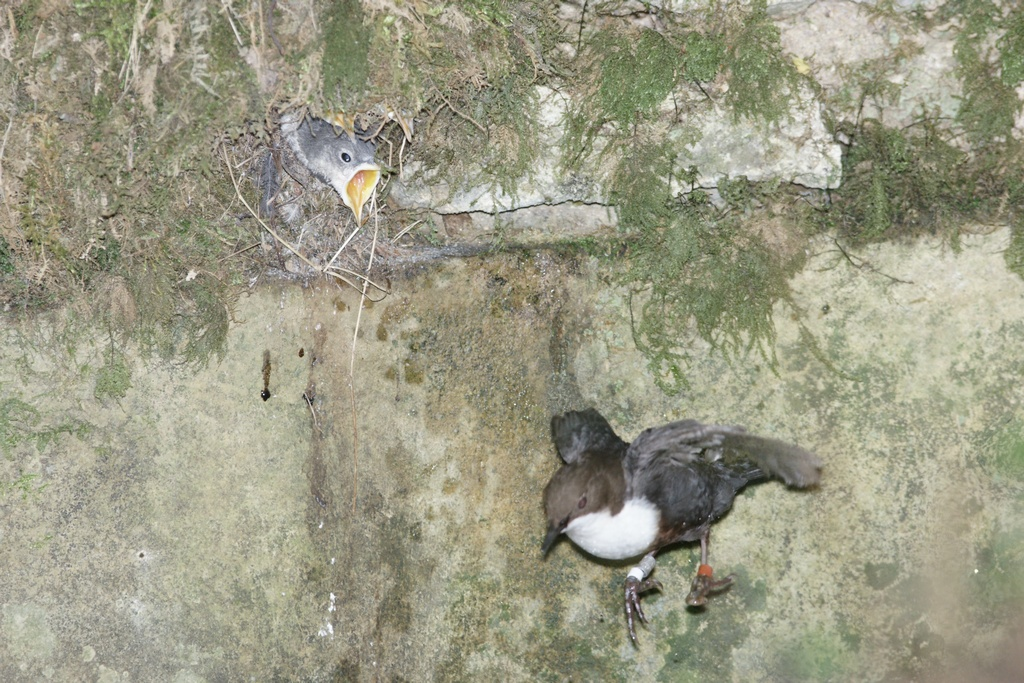
\includegraphics[width=0.6\linewidth]{images/Marzo_BaguesMance} \caption{White-throated Dipper (Cinclus cinclus)}\label{fig:unnamed-chunk-179}
\end{figure}

\begin{figure}
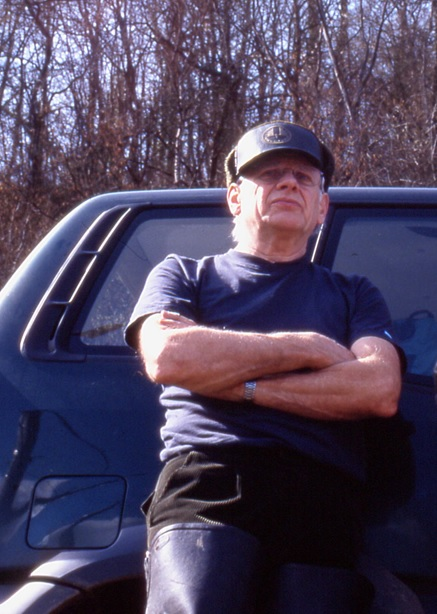
\includegraphics[width=0.6\linewidth]{images/Marzocuissardes} \caption{Gilbert Marzolin}\label{fig:unnamed-chunk-180}
\end{figure}

\hypertarget{dippers-captured-and-recaptured-between-1981-and-1987-with-known-sex-and-wing-length}{%
\section{294 dippers captured and recaptured between 1981 and 1987 with known sex and wing length}\label{dippers-captured-and-recaptured-between-1981-and-1987-with-known-sex-and-wing-length}}

\begin{tabular}{r|r|r|r|r|r|r|l|r}
\hline
year\_1981 & year\_1982 & year\_1983 & year\_1984 & year\_1985 & year\_1986 & year\_1987 & sex & wing\_length\\
\hline
1 & 1 & 1 & 1 & 1 & 1 & 0 & M & 95\\
\hline
1 & 1 & 1 & 1 & 1 & 0 & 0 & F & 88\\
\hline
1 & 1 & 1 & 1 & 0 & 0 & 0 & M & 94\\
\hline
1 & 1 & 1 & 1 & 0 & 0 & 0 & F & 85\\
\hline
1 & 1 & 0 & 1 & 1 & 1 & 0 & F & 86\\
\hline
1 & 1 & 0 & 0 & 0 & 0 & 0 & M & 97\\
\hline
1 & 1 & 0 & 0 & 0 & 0 & 0 & M & 96\\
\hline
1 & 1 & 0 & 0 & 0 & 0 & 0 & M & 98\\
\hline
1 & 1 & 0 & 0 & 0 & 0 & 0 & M & 96\\
\hline
1 & 1 & 0 & 0 & 0 & 0 & 0 & F & 89\\
\hline
1 & 1 & 0 & 0 & 0 & 0 & 0 & F & 86\\
\hline
1 & 0 & 1 & 0 & 0 & 0 & 0 & M & 98\\
\hline
1 & 0 & 1 & 0 & 0 & 0 & 0 & F & 92\\
\hline
1 & 0 & 0 & 0 & 0 & 0 & 0 & M & 97\\
\hline
1 & 0 & 0 & 0 & 0 & 0 & 0 & M & 96\\
\hline
1 & 0 & 0 & 0 & 0 & 0 & 0 & M & 95\\
\hline
1 & 0 & 0 & 0 & 0 & 0 & 0 & M & 98\\
\hline
1 & 0 & 0 & 0 & 0 & 0 & 0 & M & 96\\
\hline
1 & 0 & 0 & 0 & 0 & 0 & 0 & F & 91\\
\hline
1 & 0 & 0 & 0 & 0 & 0 & 0 & F & 89\\
\hline
1 & 0 & 0 & 0 & 0 & 0 & 0 & F & 87\\
\hline
1 & 0 & 0 & 0 & 0 & 0 & 0 & F & 90\\
\hline
0 & 1 & 1 & 1 & 1 & 1 & 1 & F & 87\\
\hline
0 & 1 & 1 & 1 & 1 & 1 & 1 & F & 86\\
\hline
0 & 1 & 1 & 1 & 1 & 1 & 0 & F & 88\\
\hline
0 & 1 & 1 & 1 & 1 & 0 & 0 & M & 99\\
\hline
0 & 1 & 1 & 1 & 1 & 0 & 0 & F & 84\\
\hline
0 & 1 & 1 & 1 & 1 & 0 & 0 & F & 87\\
\hline
0 & 1 & 1 & 1 & 0 & 0 & 0 & M & 96\\
\hline
0 & 1 & 1 & 1 & 0 & 0 & 0 & F & 89\\
\hline
0 & 1 & 1 & 0 & 1 & 1 & 0 & F & 89\\
\hline
0 & 1 & 1 & 0 & 0 & 0 & 0 & M & 97\\
\hline
0 & 1 & 1 & 0 & 0 & 0 & 0 & M & 91\\
\hline
0 & 1 & 1 & 0 & 0 & 0 & 0 & M & 98\\
\hline
0 & 1 & 1 & 0 & 0 & 0 & 0 & M & 97\\
\hline
0 & 1 & 1 & 0 & 0 & 0 & 0 & M & 94\\
\hline
0 & 1 & 1 & 0 & 0 & 0 & 0 & M & 90\\
\hline
0 & 1 & 1 & 0 & 0 & 0 & 0 & M & 93\\
\hline
0 & 1 & 1 & 0 & 0 & 0 & 0 & F & 91\\
\hline
0 & 1 & 1 & 0 & 0 & 0 & 0 & F & 84\\
\hline
0 & 1 & 1 & 0 & 0 & 0 & 0 & F & 89\\
\hline
0 & 1 & 1 & 0 & 0 & 0 & 0 & F & 89\\
\hline
0 & 1 & 0 & 0 & 0 & 0 & 0 & M & 94\\
\hline
0 & 1 & 0 & 0 & 0 & 0 & 0 & M & 96\\
\hline
0 & 1 & 0 & 0 & 0 & 0 & 0 & M & 93\\
\hline
0 & 1 & 0 & 0 & 0 & 0 & 0 & M & 92\\
\hline
0 & 1 & 0 & 0 & 0 & 0 & 0 & M & 96\\
\hline
0 & 1 & 0 & 0 & 0 & 0 & 0 & M & 97\\
\hline
0 & 1 & 0 & 0 & 0 & 0 & 0 & M & 94\\
\hline
0 & 1 & 0 & 0 & 0 & 0 & 0 & M & 98\\
\hline
0 & 1 & 0 & 0 & 0 & 0 & 0 & M & 97\\
\hline
0 & 1 & 0 & 0 & 0 & 0 & 0 & M & 96\\
\hline
0 & 1 & 0 & 0 & 0 & 0 & 0 & M & 98\\
\hline
0 & 1 & 0 & 0 & 0 & 0 & 0 & F & 88\\
\hline
0 & 1 & 0 & 0 & 0 & 0 & 0 & F & 88\\
\hline
0 & 1 & 0 & 0 & 0 & 0 & 0 & F & 88\\
\hline
0 & 1 & 0 & 0 & 0 & 0 & 0 & F & 86\\
\hline
0 & 1 & 0 & 0 & 0 & 0 & 0 & F & 93\\
\hline
0 & 1 & 0 & 0 & 0 & 0 & 0 & F & 85\\
\hline
0 & 1 & 0 & 0 & 0 & 0 & 0 & F & 88\\
\hline
0 & 1 & 0 & 0 & 0 & 0 & 0 & F & 88\\
\hline
0 & 1 & 0 & 0 & 0 & 0 & 0 & F & 86\\
\hline
0 & 1 & 0 & 0 & 0 & 0 & 0 & F & 88\\
\hline
0 & 1 & 0 & 0 & 0 & 0 & 0 & F & 88\\
\hline
0 & 1 & 0 & 0 & 0 & 0 & 0 & F & 89\\
\hline
0 & 1 & 0 & 0 & 0 & 0 & 0 & F & 86\\
\hline
0 & 1 & 0 & 0 & 0 & 0 & 0 & F & 88\\
\hline
0 & 1 & 0 & 0 & 0 & 0 & 0 & F & 88\\
\hline
0 & 1 & 0 & 0 & 0 & 0 & 0 & F & 84\\
\hline
0 & 1 & 0 & 0 & 0 & 0 & 0 & F & 87\\
\hline
0 & 1 & 0 & 0 & 0 & 0 & 0 & F & 88\\
\hline
0 & 0 & 1 & 1 & 1 & 1 & 1 & F & 89\\
\hline
0 & 0 & 1 & 1 & 1 & 1 & 1 & F & 87\\
\hline
0 & 0 & 1 & 1 & 1 & 1 & 0 & M & 96\\
\hline
0 & 0 & 1 & 1 & 1 & 1 & 0 & F & 85\\
\hline
0 & 0 & 1 & 1 & 1 & 0 & 0 & M & 98\\
\hline
0 & 0 & 1 & 1 & 1 & 0 & 0 & M & 94\\
\hline
0 & 0 & 1 & 1 & 1 & 0 & 0 & M & 94\\
\hline
0 & 0 & 1 & 1 & 1 & 0 & 0 & M & 99\\
\hline
0 & 0 & 1 & 1 & 1 & 0 & 0 & F & 90\\
\hline
0 & 0 & 1 & 1 & 1 & 0 & 0 & F & 86\\
\hline
0 & 0 & 1 & 1 & 0 & 0 & 0 & M & 96\\
\hline
0 & 0 & 1 & 1 & 0 & 0 & 0 & M & 97\\
\hline
0 & 0 & 1 & 1 & 0 & 0 & 0 & M & 98\\
\hline
0 & 0 & 1 & 1 & 0 & 0 & 0 & M & 93\\
\hline
0 & 0 & 1 & 1 & 0 & 0 & 0 & M & 94\\
\hline
0 & 0 & 1 & 1 & 0 & 0 & 0 & M & 97\\
\hline
0 & 0 & 1 & 1 & 0 & 0 & 0 & M & 98\\
\hline
0 & 0 & 1 & 1 & 0 & 0 & 0 & M & 96\\
\hline
0 & 0 & 1 & 1 & 0 & 0 & 0 & F & 89\\
\hline
0 & 0 & 1 & 1 & 0 & 0 & 0 & F & 88\\
\hline
0 & 0 & 1 & 1 & 0 & 0 & 0 & F & 90\\
\hline
0 & 0 & 1 & 1 & 0 & 0 & 0 & F & 87\\
\hline
0 & 0 & 1 & 0 & 1 & 1 & 0 & M & 95\\
\hline
0 & 0 & 1 & 0 & 0 & 0 & 0 & M & 93\\
\hline
0 & 0 & 1 & 0 & 0 & 0 & 0 & M & 97\\
\hline
0 & 0 & 1 & 0 & 0 & 0 & 0 & M & 97\\
\hline
0 & 0 & 1 & 0 & 0 & 0 & 0 & M & 99\\
\hline
0 & 0 & 1 & 0 & 0 & 0 & 0 & M & 96\\
\hline
0 & 0 & 1 & 0 & 0 & 0 & 0 & M & 94\\
\hline
0 & 0 & 1 & 0 & 0 & 0 & 0 & M & 95\\
\hline
0 & 0 & 1 & 0 & 0 & 0 & 0 & M & 100\\
\hline
0 & 0 & 1 & 0 & 0 & 0 & 0 & M & 92\\
\hline
0 & 0 & 1 & 0 & 0 & 0 & 0 & M & 96\\
\hline
0 & 0 & 1 & 0 & 0 & 0 & 0 & M & 97\\
\hline
0 & 0 & 1 & 0 & 0 & 0 & 0 & F & 88\\
\hline
0 & 0 & 1 & 0 & 0 & 0 & 0 & F & 89\\
\hline
0 & 0 & 1 & 0 & 0 & 0 & 0 & F & 91\\
\hline
0 & 0 & 1 & 0 & 0 & 0 & 0 & F & 90\\
\hline
0 & 0 & 1 & 0 & 0 & 0 & 0 & F & 88\\
\hline
0 & 0 & 1 & 0 & 0 & 0 & 0 & F & 91\\
\hline
0 & 0 & 1 & 0 & 0 & 0 & 0 & F & 89\\
\hline
0 & 0 & 1 & 0 & 0 & 0 & 0 & F & 87\\
\hline
0 & 0 & 1 & 0 & 0 & 0 & 0 & F & 90\\
\hline
0 & 0 & 1 & 0 & 0 & 0 & 0 & F & 84\\
\hline
0 & 0 & 1 & 0 & 0 & 0 & 0 & F & 86\\
\hline
0 & 0 & 1 & 0 & 0 & 0 & 0 & F & 86\\
\hline
0 & 0 & 1 & 0 & 0 & 0 & 0 & F & 87\\
\hline
0 & 0 & 1 & 0 & 0 & 0 & 0 & F & 89\\
\hline
0 & 0 & 1 & 0 & 0 & 0 & 0 & F & 88\\
\hline
0 & 0 & 1 & 0 & 0 & 0 & 0 & F & 85\\
\hline
0 & 0 & 1 & 0 & 0 & 0 & 0 & F & 90\\
\hline
0 & 0 & 1 & 0 & 0 & 0 & 0 & F & 86\\
\hline
0 & 0 & 0 & 1 & 1 & 1 & 1 & M & 98\\
\hline
0 & 0 & 0 & 1 & 1 & 1 & 1 & M & 100\\
\hline
0 & 0 & 0 & 1 & 1 & 1 & 1 & M & 94\\
\hline
0 & 0 & 0 & 1 & 1 & 1 & 1 & M & 97\\
\hline
0 & 0 & 0 & 1 & 1 & 1 & 1 & M & 96\\
\hline
0 & 0 & 0 & 1 & 1 & 1 & 1 & M & 95\\
\hline
0 & 0 & 0 & 1 & 1 & 1 & 1 & F & 85\\
\hline
0 & 0 & 0 & 1 & 1 & 1 & 1 & F & 85\\
\hline
0 & 0 & 0 & 1 & 1 & 1 & 0 & M & 93\\
\hline
0 & 0 & 0 & 1 & 1 & 1 & 0 & M & 99\\
\hline
0 & 0 & 0 & 1 & 1 & 1 & 0 & M & 95\\
\hline
0 & 0 & 0 & 1 & 1 & 1 & 0 & F & 86\\
\hline
0 & 0 & 0 & 1 & 1 & 1 & 0 & F & 85\\
\hline
0 & 0 & 0 & 1 & 1 & 1 & 0 & F & 92\\
\hline
0 & 0 & 0 & 1 & 1 & 1 & 0 & F & 89\\
\hline
0 & 0 & 0 & 1 & 1 & 0 & 0 & M & 97\\
\hline
0 & 0 & 0 & 1 & 1 & 0 & 0 & M & 92\\
\hline
0 & 0 & 0 & 1 & 1 & 0 & 0 & M & 96\\
\hline
0 & 0 & 0 & 1 & 1 & 0 & 0 & M & 95\\
\hline
0 & 0 & 0 & 1 & 1 & 0 & 0 & M & 94\\
\hline
0 & 0 & 0 & 1 & 1 & 0 & 0 & M & 95\\
\hline
0 & 0 & 0 & 1 & 1 & 0 & 0 & F & 88\\
\hline
0 & 0 & 0 & 1 & 1 & 0 & 0 & F & 88\\
\hline
0 & 0 & 0 & 1 & 1 & 0 & 0 & F & 87\\
\hline
0 & 0 & 0 & 1 & 1 & 0 & 0 & F & 87\\
\hline
0 & 0 & 0 & 1 & 1 & 0 & 0 & F & 87\\
\hline
0 & 0 & 0 & 1 & 0 & 1 & 1 & F & 88\\
\hline
0 & 0 & 0 & 1 & 0 & 0 & 1 & M & 96\\
\hline
0 & 0 & 0 & 1 & 0 & 0 & 1 & F & 87\\
\hline
0 & 0 & 0 & 1 & 0 & 0 & 0 & M & 94\\
\hline
0 & 0 & 0 & 1 & 0 & 0 & 0 & M & 92\\
\hline
0 & 0 & 0 & 1 & 0 & 0 & 0 & M & 96\\
\hline
0 & 0 & 0 & 1 & 0 & 0 & 0 & M & 95\\
\hline
0 & 0 & 0 & 1 & 0 & 0 & 0 & M & 97\\
\hline
0 & 0 & 0 & 1 & 0 & 0 & 0 & M & 95\\
\hline
0 & 0 & 0 & 1 & 0 & 0 & 0 & F & 89\\
\hline
0 & 0 & 0 & 1 & 0 & 0 & 0 & F & 89\\
\hline
0 & 0 & 0 & 1 & 0 & 0 & 0 & F & 88\\
\hline
0 & 0 & 0 & 1 & 0 & 0 & 0 & F & 88\\
\hline
0 & 0 & 0 & 1 & 0 & 0 & 0 & F & 92\\
\hline
0 & 0 & 0 & 1 & 0 & 0 & 0 & F & 88\\
\hline
0 & 0 & 0 & 1 & 0 & 0 & 0 & F & 89\\
\hline
0 & 0 & 0 & 1 & 0 & 0 & 0 & F & 88\\
\hline
0 & 0 & 0 & 1 & 0 & 0 & 0 & F & 87\\
\hline
0 & 0 & 0 & 1 & 0 & 0 & 0 & F & 88\\
\hline
0 & 0 & 0 & 0 & 1 & 1 & 1 & M & 94\\
\hline
0 & 0 & 0 & 0 & 1 & 1 & 1 & M & 96\\
\hline
0 & 0 & 0 & 0 & 1 & 1 & 1 & M & 94\\
\hline
0 & 0 & 0 & 0 & 1 & 1 & 1 & M & 100\\
\hline
0 & 0 & 0 & 0 & 1 & 1 & 1 & M & 95\\
\hline
0 & 0 & 0 & 0 & 1 & 1 & 1 & M & 96\\
\hline
0 & 0 & 0 & 0 & 1 & 1 & 1 & M & 97\\
\hline
0 & 0 & 0 & 0 & 1 & 1 & 1 & M & 97\\
\hline
0 & 0 & 0 & 0 & 1 & 1 & 1 & M & 95\\
\hline
0 & 0 & 0 & 0 & 1 & 1 & 1 & M & 98\\
\hline
0 & 0 & 0 & 0 & 1 & 1 & 1 & F & 87\\
\hline
0 & 0 & 0 & 0 & 1 & 1 & 1 & F & 85\\
\hline
0 & 0 & 0 & 0 & 1 & 1 & 1 & F & 87\\
\hline
0 & 0 & 0 & 0 & 1 & 1 & 1 & F & 89\\
\hline
0 & 0 & 0 & 0 & 1 & 1 & 1 & F & 87\\
\hline
0 & 0 & 0 & 0 & 1 & 1 & 1 & F & 91\\
\hline
0 & 0 & 0 & 0 & 1 & 1 & 0 & M & 96\\
\hline
0 & 0 & 0 & 0 & 1 & 1 & 0 & M & 97\\
\hline
0 & 0 & 0 & 0 & 1 & 1 & 0 & M & 95\\
\hline
0 & 0 & 0 & 0 & 1 & 1 & 0 & F & 86\\
\hline
0 & 0 & 0 & 0 & 1 & 1 & 0 & F & 87\\
\hline
0 & 0 & 0 & 0 & 1 & 1 & 0 & F & 88\\
\hline
0 & 0 & 0 & 0 & 1 & 1 & 0 & F & 90\\
\hline
0 & 0 & 0 & 0 & 1 & 1 & 0 & F & 90\\
\hline
0 & 0 & 0 & 0 & 1 & 1 & 0 & F & 88\\
\hline
0 & 0 & 0 & 0 & 1 & 0 & 0 & M & 96\\
\hline
0 & 0 & 0 & 0 & 1 & 0 & 0 & M & 98\\
\hline
0 & 0 & 0 & 0 & 1 & 0 & 0 & M & 94\\
\hline
0 & 0 & 0 & 0 & 1 & 0 & 0 & M & 98\\
\hline
0 & 0 & 0 & 0 & 1 & 0 & 0 & M & 97\\
\hline
0 & 0 & 0 & 0 & 1 & 0 & 0 & M & 97\\
\hline
0 & 0 & 0 & 0 & 1 & 0 & 0 & M & 94\\
\hline
0 & 0 & 0 & 0 & 1 & 0 & 0 & M & 98\\
\hline
0 & 0 & 0 & 0 & 1 & 0 & 0 & M & 94\\
\hline
0 & 0 & 0 & 0 & 1 & 0 & 0 & F & 89\\
\hline
0 & 0 & 0 & 0 & 1 & 0 & 0 & F & 88\\
\hline
0 & 0 & 0 & 0 & 1 & 0 & 0 & F & 89\\
\hline
0 & 0 & 0 & 0 & 1 & 0 & 0 & F & 92\\
\hline
0 & 0 & 0 & 0 & 1 & 0 & 0 & F & 91\\
\hline
0 & 0 & 0 & 0 & 1 & 0 & 0 & F & 85\\
\hline
0 & 0 & 0 & 0 & 1 & 0 & 0 & F & 85\\
\hline
0 & 0 & 0 & 0 & 0 & 1 & 1 & M & 94\\
\hline
0 & 0 & 0 & 0 & 0 & 1 & 1 & M & 99\\
\hline
0 & 0 & 0 & 0 & 0 & 1 & 1 & M & 96\\
\hline
0 & 0 & 0 & 0 & 0 & 1 & 1 & M & 97\\
\hline
0 & 0 & 0 & 0 & 0 & 1 & 1 & M & 92\\
\hline
0 & 0 & 0 & 0 & 0 & 1 & 1 & M & 96\\
\hline
0 & 0 & 0 & 0 & 0 & 1 & 1 & M & 90\\
\hline
0 & 0 & 0 & 0 & 0 & 1 & 1 & M & 93\\
\hline
0 & 0 & 0 & 0 & 0 & 1 & 1 & M & 95\\
\hline
0 & 0 & 0 & 0 & 0 & 1 & 1 & M & 94\\
\hline
0 & 0 & 0 & 0 & 0 & 1 & 1 & M & 96\\
\hline
0 & 0 & 0 & 0 & 0 & 1 & 1 & M & 96\\
\hline
0 & 0 & 0 & 0 & 0 & 1 & 1 & F & 87\\
\hline
0 & 0 & 0 & 0 & 0 & 1 & 1 & F & 87\\
\hline
0 & 0 & 0 & 0 & 0 & 1 & 1 & F & 88\\
\hline
0 & 0 & 0 & 0 & 0 & 1 & 1 & F & 88\\
\hline
0 & 0 & 0 & 0 & 0 & 1 & 1 & F & 88\\
\hline
0 & 0 & 0 & 0 & 0 & 1 & 1 & F & 86\\
\hline
0 & 0 & 0 & 0 & 0 & 1 & 1 & F & 88\\
\hline
0 & 0 & 0 & 0 & 0 & 1 & 1 & F & 88\\
\hline
0 & 0 & 0 & 0 & 0 & 1 & 1 & F & 87\\
\hline
0 & 0 & 0 & 0 & 0 & 1 & 1 & F & 90\\
\hline
0 & 0 & 0 & 0 & 0 & 1 & 1 & F & 91\\
\hline
0 & 0 & 0 & 0 & 0 & 1 & 0 & M & 95\\
\hline
0 & 0 & 0 & 0 & 0 & 1 & 0 & M & 98\\
\hline
0 & 0 & 0 & 0 & 0 & 1 & 0 & M & 95\\
\hline
0 & 0 & 0 & 0 & 0 & 1 & 0 & M & 96\\
\hline
0 & 0 & 0 & 0 & 0 & 1 & 0 & M & 99\\
\hline
0 & 0 & 0 & 0 & 0 & 1 & 0 & M & 98\\
\hline
0 & 0 & 0 & 0 & 0 & 1 & 0 & M & 91\\
\hline
0 & 0 & 0 & 0 & 0 & 1 & 0 & M & 94\\
\hline
0 & 0 & 0 & 0 & 0 & 1 & 0 & M & 96\\
\hline
0 & 0 & 0 & 0 & 0 & 1 & 0 & M & 99\\
\hline
0 & 0 & 0 & 0 & 0 & 1 & 0 & M & 91\\
\hline
0 & 0 & 0 & 0 & 0 & 1 & 0 & F & 91\\
\hline
0 & 0 & 0 & 0 & 0 & 1 & 0 & F & 84\\
\hline
0 & 0 & 0 & 0 & 0 & 1 & 0 & F & 88\\
\hline
0 & 0 & 0 & 0 & 0 & 1 & 0 & F & 86\\
\hline
0 & 0 & 0 & 0 & 0 & 1 & 0 & F & 89\\
\hline
0 & 0 & 0 & 0 & 0 & 1 & 0 & F & 90\\
\hline
0 & 0 & 0 & 0 & 0 & 1 & 0 & F & 88\\
\hline
0 & 0 & 0 & 0 & 0 & 1 & 0 & F & 87\\
\hline
0 & 0 & 0 & 0 & 0 & 1 & 0 & F & 90\\
\hline
0 & 0 & 0 & 0 & 0 & 1 & 0 & F & 88\\
\hline
0 & 0 & 0 & 0 & 0 & 1 & 0 & F & 92\\
\hline
0 & 0 & 0 & 0 & 0 & 1 & 0 & F & 88\\
\hline
0 & 0 & 0 & 0 & 0 & 0 & 1 & M & 97\\
\hline
0 & 0 & 0 & 0 & 0 & 0 & 1 & M & 97\\
\hline
0 & 0 & 0 & 0 & 0 & 0 & 1 & M & 98\\
\hline
0 & 0 & 0 & 0 & 0 & 0 & 1 & M & 94\\
\hline
0 & 0 & 0 & 0 & 0 & 0 & 1 & M & 95\\
\hline
0 & 0 & 0 & 0 & 0 & 0 & 1 & M & 97\\
\hline
0 & 0 & 0 & 0 & 0 & 0 & 1 & M & 97\\
\hline
0 & 0 & 0 & 0 & 0 & 0 & 1 & M & 96\\
\hline
0 & 0 & 0 & 0 & 0 & 0 & 1 & M & 94\\
\hline
0 & 0 & 0 & 0 & 0 & 0 & 1 & M & 95\\
\hline
0 & 0 & 0 & 0 & 0 & 0 & 1 & M & 94\\
\hline
0 & 0 & 0 & 0 & 0 & 0 & 1 & M & 94\\
\hline
0 & 0 & 0 & 0 & 0 & 0 & 1 & M & 94\\
\hline
0 & 0 & 0 & 0 & 0 & 0 & 1 & M & 94\\
\hline
0 & 0 & 0 & 0 & 0 & 0 & 1 & M & 96\\
\hline
0 & 0 & 0 & 0 & 0 & 0 & 1 & M & 97\\
\hline
0 & 0 & 0 & 0 & 0 & 0 & 1 & M & 95\\
\hline
0 & 0 & 0 & 0 & 0 & 0 & 1 & F & 86\\
\hline
0 & 0 & 0 & 0 & 0 & 0 & 1 & F & 87\\
\hline
0 & 0 & 0 & 0 & 0 & 0 & 1 & F & 88\\
\hline
0 & 0 & 0 & 0 & 0 & 0 & 1 & F & 90\\
\hline
0 & 0 & 0 & 0 & 0 & 0 & 1 & F & 90\\
\hline
0 & 0 & 0 & 0 & 0 & 0 & 1 & F & 88\\
\hline
0 & 0 & 0 & 0 & 0 & 0 & 1 & F & 88\\
\hline
0 & 0 & 0 & 0 & 0 & 0 & 1 & F & 88\\
\hline
0 & 0 & 0 & 0 & 0 & 0 & 1 & F & 91\\
\hline
0 & 0 & 0 & 0 & 0 & 0 & 1 & F & 90\\
\hline
0 & 0 & 0 & 0 & 0 & 0 & 1 & F & 86\\
\hline
0 & 0 & 0 & 0 & 0 & 0 & 1 & F & 88\\
\hline
0 & 0 & 0 & 0 & 0 & 0 & 1 & F & 90\\
\hline
0 & 0 & 0 & 0 & 0 & 0 & 1 & F & 88\\
\hline
0 & 0 & 0 & 0 & 0 & 0 & 1 & F & 90\\
\hline
0 & 0 & 0 & 0 & 0 & 0 & 1 & F & 90\\
\hline
0 & 0 & 0 & 0 & 0 & 0 & 1 & F & 92\\
\hline
0 & 0 & 0 & 0 & 0 & 0 & 1 & F & 86\\
\hline
0 & 0 & 0 & 0 & 0 & 0 & 1 & F & 89\\
\hline
0 & 0 & 0 & 0 & 0 & 0 & 1 & F & 88\\
\hline
0 & 0 & 0 & 0 & 0 & 0 & 1 & F & 90\\
\hline
0 & 0 & 0 & 0 & 0 & 0 & 1 & F & 93\\
\hline
\end{tabular}

\hypertarget{back-to-nimble.}{%
\section{Back to Nimble.}\label{back-to-nimble.}}

\hypertarget{our-model-so-far-phi-p}{%
\subsection{\texorpdfstring{Our model so far \((\phi, p)\)}{Our model so far (\textbackslash phi, p)}}\label{our-model-so-far-phi-p}}

\begin{Shaded}
\begin{Highlighting}[]
\NormalTok{hmm.phip }\OtherTok{\textless{}{-}} \FunctionTok{nimbleCode}\NormalTok{(\{}
\NormalTok{  phi }\SpecialCharTok{\textasciitilde{}} \FunctionTok{dunif}\NormalTok{(}\DecValTok{0}\NormalTok{, }\DecValTok{1}\NormalTok{) }\CommentTok{\# prior survival}
\NormalTok{  p }\SpecialCharTok{\textasciitilde{}} \FunctionTok{dunif}\NormalTok{(}\DecValTok{0}\NormalTok{, }\DecValTok{1}\NormalTok{) }\CommentTok{\# prior detection}
  \CommentTok{\# likelihood}
\NormalTok{  gamma[}\DecValTok{1}\NormalTok{,}\DecValTok{1}\NormalTok{] }\OtherTok{\textless{}{-}}\NormalTok{ phi      }\CommentTok{\# Pr(alive t {-}\textgreater{} alive t+1)}
\NormalTok{  gamma[}\DecValTok{1}\NormalTok{,}\DecValTok{2}\NormalTok{] }\OtherTok{\textless{}{-}} \DecValTok{1} \SpecialCharTok{{-}}\NormalTok{ phi  }\CommentTok{\# Pr(alive t {-}\textgreater{} dead t+1)}
\NormalTok{  gamma[}\DecValTok{2}\NormalTok{,}\DecValTok{1}\NormalTok{] }\OtherTok{\textless{}{-}} \DecValTok{0}        \CommentTok{\# Pr(dead t {-}\textgreater{} alive t+1)}
\NormalTok{  gamma[}\DecValTok{2}\NormalTok{,}\DecValTok{2}\NormalTok{] }\OtherTok{\textless{}{-}} \DecValTok{1}        \CommentTok{\# Pr(dead t {-}\textgreater{} dead t+1)}
\NormalTok{  delta[}\DecValTok{1}\NormalTok{] }\OtherTok{\textless{}{-}} \DecValTok{1}          \CommentTok{\# Pr(alive t = 1) = 1}
\NormalTok{  delta[}\DecValTok{2}\NormalTok{] }\OtherTok{\textless{}{-}} \DecValTok{0}          \CommentTok{\# Pr(dead t = 1) = 0}
\NormalTok{  omega[}\DecValTok{1}\NormalTok{,}\DecValTok{1}\NormalTok{] }\OtherTok{\textless{}{-}} \DecValTok{1} \SpecialCharTok{{-}}\NormalTok{ p    }\CommentTok{\# Pr(alive t {-}\textgreater{} non{-}detected t)}
\NormalTok{  omega[}\DecValTok{1}\NormalTok{,}\DecValTok{2}\NormalTok{] }\OtherTok{\textless{}{-}}\NormalTok{ p        }\CommentTok{\# Pr(alive t {-}\textgreater{} detected t)}
\NormalTok{  omega[}\DecValTok{2}\NormalTok{,}\DecValTok{1}\NormalTok{] }\OtherTok{\textless{}{-}} \DecValTok{1}        \CommentTok{\# Pr(dead t {-}\textgreater{} non{-}detected t)}
\NormalTok{  omega[}\DecValTok{2}\NormalTok{,}\DecValTok{2}\NormalTok{] }\OtherTok{\textless{}{-}} \DecValTok{0}        \CommentTok{\# Pr(dead t {-}\textgreater{} detected t)}
  \ControlFlowTok{for}\NormalTok{ (i }\ControlFlowTok{in} \DecValTok{1}\SpecialCharTok{:}\NormalTok{N)\{}
\NormalTok{    z[i,first[i]] }\SpecialCharTok{\textasciitilde{}} \FunctionTok{dcat}\NormalTok{(delta[}\DecValTok{1}\SpecialCharTok{:}\DecValTok{2}\NormalTok{])}
    \ControlFlowTok{for}\NormalTok{ (j }\ControlFlowTok{in}\NormalTok{ (first[i]}\SpecialCharTok{+}\DecValTok{1}\NormalTok{)}\SpecialCharTok{:}\NormalTok{T)\{}
\NormalTok{      z[i,j] }\SpecialCharTok{\textasciitilde{}} \FunctionTok{dcat}\NormalTok{(gamma[z[i,j}\DecValTok{{-}1}\NormalTok{], }\DecValTok{1}\SpecialCharTok{:}\DecValTok{2}\NormalTok{])}
\NormalTok{      y[i,j] }\SpecialCharTok{\textasciitilde{}} \FunctionTok{dcat}\NormalTok{(omega[z[i,j], }\DecValTok{1}\SpecialCharTok{:}\DecValTok{2}\NormalTok{])}
\NormalTok{    \}}
\NormalTok{  \}}
\NormalTok{\})}
\end{Highlighting}
\end{Shaded}

\hypertarget{our-model-so-far-phi-p-1}{%
\subsection{\texorpdfstring{Our model so far \((\phi, p)\)}{Our model so far (\textbackslash phi, p)}}\label{our-model-so-far-phi-p-1}}

\begin{verbatim}
##     mean   sd 2.5%  50% 97.5% Rhat n.eff
## phi 0.56 0.03 0.52 0.56  0.62 1.00   500
## p   0.89 0.03 0.83 0.89  0.94 1.13   273
\end{verbatim}

\hypertarget{the-cjs-model-phi_t-p_t}{%
\subsection{\texorpdfstring{The CJS model \((\phi_t, p_t)\)}{The CJS model (\textbackslash phi\_t, p\_t)}}\label{the-cjs-model-phi_t-p_t}}

\begin{Shaded}
\begin{Highlighting}[]
\NormalTok{hmm.phitpt }\OtherTok{\textless{}{-}} \FunctionTok{nimbleCode}\NormalTok{(\{}
\NormalTok{  delta[}\DecValTok{1}\NormalTok{] }\OtherTok{\textless{}{-}} \DecValTok{1}          \CommentTok{\# Pr(alive t = 1) = 1}
\NormalTok{  delta[}\DecValTok{2}\NormalTok{] }\OtherTok{\textless{}{-}} \DecValTok{0}          \CommentTok{\# Pr(dead t = 1) = 0}
  \ControlFlowTok{for}\NormalTok{ (t }\ControlFlowTok{in} \DecValTok{1}\SpecialCharTok{:}\NormalTok{(T}\DecValTok{{-}1}\NormalTok{))\{}
\NormalTok{    phi[t] }\SpecialCharTok{\textasciitilde{}} \FunctionTok{dunif}\NormalTok{(}\DecValTok{0}\NormalTok{, }\DecValTok{1}\NormalTok{) }\CommentTok{\# prior survival \#\textless{}\textless{}}
\NormalTok{    gamma[}\DecValTok{1}\NormalTok{,}\DecValTok{1}\NormalTok{,t] }\OtherTok{\textless{}{-}}\NormalTok{ phi[t]      }\CommentTok{\# Pr(alive t {-}\textgreater{} alive t+1)}
\NormalTok{    gamma[}\DecValTok{1}\NormalTok{,}\DecValTok{2}\NormalTok{,t] }\OtherTok{\textless{}{-}} \DecValTok{1} \SpecialCharTok{{-}}\NormalTok{ phi[t]  }\CommentTok{\# Pr(alive t {-}\textgreater{} dead t+1)}
\NormalTok{    gamma[}\DecValTok{2}\NormalTok{,}\DecValTok{1}\NormalTok{,t] }\OtherTok{\textless{}{-}} \DecValTok{0}        \CommentTok{\# Pr(dead t {-}\textgreater{} alive t+1)}
\NormalTok{    gamma[}\DecValTok{2}\NormalTok{,}\DecValTok{2}\NormalTok{,t] }\OtherTok{\textless{}{-}} \DecValTok{1}        \CommentTok{\# Pr(dead t {-}\textgreater{} dead t+1)}
\NormalTok{    p[t] }\SpecialCharTok{\textasciitilde{}} \FunctionTok{dunif}\NormalTok{(}\DecValTok{0}\NormalTok{, }\DecValTok{1}\NormalTok{) }\CommentTok{\# prior detection \#\textless{}\textless{}}
\NormalTok{    omega[}\DecValTok{1}\NormalTok{,}\DecValTok{1}\NormalTok{,t] }\OtherTok{\textless{}{-}} \DecValTok{1} \SpecialCharTok{{-}}\NormalTok{ p[t]    }\CommentTok{\# Pr(alive t {-}\textgreater{} non{-}detected t)}
\NormalTok{    omega[}\DecValTok{1}\NormalTok{,}\DecValTok{2}\NormalTok{,t] }\OtherTok{\textless{}{-}}\NormalTok{ p[t]        }\CommentTok{\# Pr(alive t {-}\textgreater{} detected t)}
\NormalTok{    omega[}\DecValTok{2}\NormalTok{,}\DecValTok{1}\NormalTok{,t] }\OtherTok{\textless{}{-}} \DecValTok{1}        \CommentTok{\# Pr(dead t {-}\textgreater{} non{-}detected t)}
\NormalTok{    omega[}\DecValTok{2}\NormalTok{,}\DecValTok{2}\NormalTok{,t] }\OtherTok{\textless{}{-}} \DecValTok{0}        \CommentTok{\# Pr(dead t {-}\textgreater{} detected t)}
\NormalTok{  \}}
  \CommentTok{\# likelihood}
  \ControlFlowTok{for}\NormalTok{ (i }\ControlFlowTok{in} \DecValTok{1}\SpecialCharTok{:}\NormalTok{N)\{}
\NormalTok{    z[i,first[i]] }\SpecialCharTok{\textasciitilde{}} \FunctionTok{dcat}\NormalTok{(delta[}\DecValTok{1}\SpecialCharTok{:}\DecValTok{2}\NormalTok{])}
    \ControlFlowTok{for}\NormalTok{ (j }\ControlFlowTok{in}\NormalTok{ (first[i]}\SpecialCharTok{+}\DecValTok{1}\NormalTok{)}\SpecialCharTok{:}\NormalTok{T)\{}
\NormalTok{      z[i,j] }\SpecialCharTok{\textasciitilde{}} \FunctionTok{dcat}\NormalTok{(gamma[z[i,j}\DecValTok{{-}1}\NormalTok{], }\DecValTok{1}\SpecialCharTok{:}\DecValTok{2}\NormalTok{, j}\DecValTok{{-}1}\NormalTok{])}
\NormalTok{      y[i,j] }\SpecialCharTok{\textasciitilde{}} \FunctionTok{dcat}\NormalTok{(omega[z[i,j], }\DecValTok{1}\SpecialCharTok{:}\DecValTok{2}\NormalTok{, j}\DecValTok{{-}1}\NormalTok{])}
\NormalTok{    \}}
\NormalTok{  \}}
\NormalTok{\})}
\end{Highlighting}
\end{Shaded}

\hypertarget{the-cjs-model-phi_t-p_t-1}{%
\subsection{\texorpdfstring{The CJS model \((\phi_t, p_t)\)}{The CJS model (\textbackslash phi\_t, p\_t)}}\label{the-cjs-model-phi_t-p_t-1}}

\begin{Shaded}
\begin{Highlighting}[]
\NormalTok{hmm.phitpt }\OtherTok{\textless{}{-}} \FunctionTok{nimbleCode}\NormalTok{(\{}
\NormalTok{  delta[}\DecValTok{1}\NormalTok{] }\OtherTok{\textless{}{-}} \DecValTok{1}          \CommentTok{\# Pr(alive t = 1) = 1}
\NormalTok{  delta[}\DecValTok{2}\NormalTok{] }\OtherTok{\textless{}{-}} \DecValTok{0}          \CommentTok{\# Pr(dead t = 1) = 0}
  \ControlFlowTok{for}\NormalTok{ (t }\ControlFlowTok{in} \DecValTok{1}\SpecialCharTok{:}\NormalTok{(T}\DecValTok{{-}1}\NormalTok{))\{ }\CommentTok{\#\textless{}\textless{}}
\NormalTok{    phi[t] }\SpecialCharTok{\textasciitilde{}} \FunctionTok{dunif}\NormalTok{(}\DecValTok{0}\NormalTok{, }\DecValTok{1}\NormalTok{) }\CommentTok{\# prior survival}
\NormalTok{    gamma[}\DecValTok{1}\NormalTok{,}\DecValTok{1}\NormalTok{,t] }\OtherTok{\textless{}{-}}\NormalTok{ phi[t]      }\CommentTok{\# Pr(alive t {-}\textgreater{} alive t+1)}
\NormalTok{    gamma[}\DecValTok{1}\NormalTok{,}\DecValTok{2}\NormalTok{,t] }\OtherTok{\textless{}{-}} \DecValTok{1} \SpecialCharTok{{-}}\NormalTok{ phi[t]  }\CommentTok{\# Pr(alive t {-}\textgreater{} dead t+1)}
\NormalTok{    gamma[}\DecValTok{2}\NormalTok{,}\DecValTok{1}\NormalTok{,t] }\OtherTok{\textless{}{-}} \DecValTok{0}        \CommentTok{\# Pr(dead t {-}\textgreater{} alive t+1)}
\NormalTok{    gamma[}\DecValTok{2}\NormalTok{,}\DecValTok{2}\NormalTok{,t] }\OtherTok{\textless{}{-}} \DecValTok{1}        \CommentTok{\# Pr(dead t {-}\textgreater{} dead t+1)}
\NormalTok{    p[t] }\SpecialCharTok{\textasciitilde{}} \FunctionTok{dunif}\NormalTok{(}\DecValTok{0}\NormalTok{, }\DecValTok{1}\NormalTok{) }\CommentTok{\# prior detection}
\NormalTok{    omega[}\DecValTok{1}\NormalTok{,}\DecValTok{1}\NormalTok{,t] }\OtherTok{\textless{}{-}} \DecValTok{1} \SpecialCharTok{{-}}\NormalTok{ p[t]    }\CommentTok{\# Pr(alive t {-}\textgreater{} non{-}detected t)}
\NormalTok{    omega[}\DecValTok{1}\NormalTok{,}\DecValTok{2}\NormalTok{,t] }\OtherTok{\textless{}{-}}\NormalTok{ p[t]        }\CommentTok{\# Pr(alive t {-}\textgreater{} detected t)}
\NormalTok{    omega[}\DecValTok{2}\NormalTok{,}\DecValTok{1}\NormalTok{,t] }\OtherTok{\textless{}{-}} \DecValTok{1}        \CommentTok{\# Pr(dead t {-}\textgreater{} non{-}detected t)}
\NormalTok{    omega[}\DecValTok{2}\NormalTok{,}\DecValTok{2}\NormalTok{,t] }\OtherTok{\textless{}{-}} \DecValTok{0}        \CommentTok{\# Pr(dead t {-}\textgreater{} detected t)}
\NormalTok{  \} }\CommentTok{\#\textless{}\textless{}}
  \CommentTok{\# likelihood}
  \ControlFlowTok{for}\NormalTok{ (i }\ControlFlowTok{in} \DecValTok{1}\SpecialCharTok{:}\NormalTok{N)\{}
\NormalTok{    z[i,first[i]] }\SpecialCharTok{\textasciitilde{}} \FunctionTok{dcat}\NormalTok{(delta[}\DecValTok{1}\SpecialCharTok{:}\DecValTok{2}\NormalTok{])}
    \ControlFlowTok{for}\NormalTok{ (j }\ControlFlowTok{in}\NormalTok{ (first[i]}\SpecialCharTok{+}\DecValTok{1}\NormalTok{)}\SpecialCharTok{:}\NormalTok{T)\{}
\NormalTok{      z[i,j] }\SpecialCharTok{\textasciitilde{}} \FunctionTok{dcat}\NormalTok{(gamma[z[i,j}\DecValTok{{-}1}\NormalTok{], }\DecValTok{1}\SpecialCharTok{:}\DecValTok{2}\NormalTok{, j}\DecValTok{{-}1}\NormalTok{])}
\NormalTok{      y[i,j] }\SpecialCharTok{\textasciitilde{}} \FunctionTok{dcat}\NormalTok{(omega[z[i,j], }\DecValTok{1}\SpecialCharTok{:}\DecValTok{2}\NormalTok{, j}\DecValTok{{-}1}\NormalTok{])}
\NormalTok{    \}}
\NormalTok{  \}}
\NormalTok{\})}
\end{Highlighting}
\end{Shaded}

\hypertarget{the-cjs-model-phi_t-p_t-2}{%
\subsection{\texorpdfstring{The CJS model \((\phi_t, p_t)\)}{The CJS model (\textbackslash phi\_t, p\_t)}}\label{the-cjs-model-phi_t-p_t-2}}

\begin{Shaded}
\begin{Highlighting}[]
\NormalTok{hmm.phitpt }\OtherTok{\textless{}{-}} \FunctionTok{nimbleCode}\NormalTok{(\{}
\NormalTok{  delta[}\DecValTok{1}\NormalTok{] }\OtherTok{\textless{}{-}} \DecValTok{1}          \CommentTok{\# Pr(alive t = 1) = 1}
\NormalTok{  delta[}\DecValTok{2}\NormalTok{] }\OtherTok{\textless{}{-}} \DecValTok{0}          \CommentTok{\# Pr(dead t = 1) = 0}
  \ControlFlowTok{for}\NormalTok{ (t }\ControlFlowTok{in} \DecValTok{1}\SpecialCharTok{:}\NormalTok{(T}\DecValTok{{-}1}\NormalTok{))\{}
\NormalTok{    phi[t] }\SpecialCharTok{\textasciitilde{}} \FunctionTok{dunif}\NormalTok{(}\DecValTok{0}\NormalTok{, }\DecValTok{1}\NormalTok{) }\CommentTok{\# prior survival}
\NormalTok{    gamma[}\DecValTok{1}\NormalTok{,}\DecValTok{1}\NormalTok{,t] }\OtherTok{\textless{}{-}}\NormalTok{ phi[t]      }\CommentTok{\# Pr(alive t {-}\textgreater{} alive t+1) \#\textless{}\textless{}}
\NormalTok{    gamma[}\DecValTok{1}\NormalTok{,}\DecValTok{2}\NormalTok{,t] }\OtherTok{\textless{}{-}} \DecValTok{1} \SpecialCharTok{{-}}\NormalTok{ phi[t]  }\CommentTok{\# Pr(alive t {-}\textgreater{} dead t+1) \#\textless{}\textless{}}
\NormalTok{    gamma[}\DecValTok{2}\NormalTok{,}\DecValTok{1}\NormalTok{,t] }\OtherTok{\textless{}{-}} \DecValTok{0}        \CommentTok{\# Pr(dead t {-}\textgreater{} alive t+1) \#\textless{}\textless{}}
\NormalTok{    gamma[}\DecValTok{2}\NormalTok{,}\DecValTok{2}\NormalTok{,t] }\OtherTok{\textless{}{-}} \DecValTok{1}        \CommentTok{\# Pr(dead t {-}\textgreater{} dead t+1) \#\textless{}\textless{}}
\NormalTok{    p[t] }\SpecialCharTok{\textasciitilde{}} \FunctionTok{dunif}\NormalTok{(}\DecValTok{0}\NormalTok{, }\DecValTok{1}\NormalTok{) }\CommentTok{\# prior detection}
\NormalTok{    omega[}\DecValTok{1}\NormalTok{,}\DecValTok{1}\NormalTok{,t] }\OtherTok{\textless{}{-}} \DecValTok{1} \SpecialCharTok{{-}}\NormalTok{ p[t]    }\CommentTok{\# Pr(alive t {-}\textgreater{} non{-}detected t)}
\NormalTok{    omega[}\DecValTok{1}\NormalTok{,}\DecValTok{2}\NormalTok{,t] }\OtherTok{\textless{}{-}}\NormalTok{ p[t]        }\CommentTok{\# Pr(alive t {-}\textgreater{} detected t)}
\NormalTok{    omega[}\DecValTok{2}\NormalTok{,}\DecValTok{1}\NormalTok{,t] }\OtherTok{\textless{}{-}} \DecValTok{1}        \CommentTok{\# Pr(dead t {-}\textgreater{} non{-}detected t)}
\NormalTok{    omega[}\DecValTok{2}\NormalTok{,}\DecValTok{2}\NormalTok{,t] }\OtherTok{\textless{}{-}} \DecValTok{0}        \CommentTok{\# Pr(dead t {-}\textgreater{} detected t)}
\NormalTok{  \}}
  \CommentTok{\# likelihood}
  \ControlFlowTok{for}\NormalTok{ (i }\ControlFlowTok{in} \DecValTok{1}\SpecialCharTok{:}\NormalTok{N)\{}
\NormalTok{    z[i,first[i]] }\SpecialCharTok{\textasciitilde{}} \FunctionTok{dcat}\NormalTok{(delta[}\DecValTok{1}\SpecialCharTok{:}\DecValTok{2}\NormalTok{])}
    \ControlFlowTok{for}\NormalTok{ (j }\ControlFlowTok{in}\NormalTok{ (first[i]}\SpecialCharTok{+}\DecValTok{1}\NormalTok{)}\SpecialCharTok{:}\NormalTok{T)\{}
\NormalTok{      z[i,j] }\SpecialCharTok{\textasciitilde{}} \FunctionTok{dcat}\NormalTok{(gamma[z[i,j}\DecValTok{{-}1}\NormalTok{], }\DecValTok{1}\SpecialCharTok{:}\DecValTok{2}\NormalTok{, j}\DecValTok{{-}1}\NormalTok{])}
\NormalTok{      y[i,j] }\SpecialCharTok{\textasciitilde{}} \FunctionTok{dcat}\NormalTok{(omega[z[i,j], }\DecValTok{1}\SpecialCharTok{:}\DecValTok{2}\NormalTok{, j}\DecValTok{{-}1}\NormalTok{])}
\NormalTok{    \}}
\NormalTok{  \}}
\NormalTok{\})}
\end{Highlighting}
\end{Shaded}

\hypertarget{the-cjs-model-phi_t-p_t-3}{%
\subsection{\texorpdfstring{The CJS model \((\phi_t, p_t)\)}{The CJS model (\textbackslash phi\_t, p\_t)}}\label{the-cjs-model-phi_t-p_t-3}}

\begin{Shaded}
\begin{Highlighting}[]
\NormalTok{hmm.phitpt }\OtherTok{\textless{}{-}} \FunctionTok{nimbleCode}\NormalTok{(\{}
\NormalTok{  delta[}\DecValTok{1}\NormalTok{] }\OtherTok{\textless{}{-}} \DecValTok{1}          \CommentTok{\# Pr(alive t = 1) = 1}
\NormalTok{  delta[}\DecValTok{2}\NormalTok{] }\OtherTok{\textless{}{-}} \DecValTok{0}          \CommentTok{\# Pr(dead t = 1) = 0}
  \ControlFlowTok{for}\NormalTok{ (t }\ControlFlowTok{in} \DecValTok{1}\SpecialCharTok{:}\NormalTok{(T}\DecValTok{{-}1}\NormalTok{))\{}
\NormalTok{    phi[t] }\SpecialCharTok{\textasciitilde{}} \FunctionTok{dunif}\NormalTok{(}\DecValTok{0}\NormalTok{, }\DecValTok{1}\NormalTok{) }\CommentTok{\# prior survival}
\NormalTok{    gamma[}\DecValTok{1}\NormalTok{,}\DecValTok{1}\NormalTok{,t] }\OtherTok{\textless{}{-}}\NormalTok{ phi[t]      }\CommentTok{\# Pr(alive t {-}\textgreater{} alive t+1)}
\NormalTok{    gamma[}\DecValTok{1}\NormalTok{,}\DecValTok{2}\NormalTok{,t] }\OtherTok{\textless{}{-}} \DecValTok{1} \SpecialCharTok{{-}}\NormalTok{ phi[t]  }\CommentTok{\# Pr(alive t {-}\textgreater{} dead t+1)}
\NormalTok{    gamma[}\DecValTok{2}\NormalTok{,}\DecValTok{1}\NormalTok{,t] }\OtherTok{\textless{}{-}} \DecValTok{0}        \CommentTok{\# Pr(dead t {-}\textgreater{} alive t+1)}
\NormalTok{    gamma[}\DecValTok{2}\NormalTok{,}\DecValTok{2}\NormalTok{,t] }\OtherTok{\textless{}{-}} \DecValTok{1}        \CommentTok{\# Pr(dead t {-}\textgreater{} dead t+1)}
\NormalTok{    p[t] }\SpecialCharTok{\textasciitilde{}} \FunctionTok{dunif}\NormalTok{(}\DecValTok{0}\NormalTok{, }\DecValTok{1}\NormalTok{) }\CommentTok{\# prior detection}
\NormalTok{    omega[}\DecValTok{1}\NormalTok{,}\DecValTok{1}\NormalTok{,t] }\OtherTok{\textless{}{-}} \DecValTok{1} \SpecialCharTok{{-}}\NormalTok{ p[t]    }\CommentTok{\# Pr(alive t {-}\textgreater{} non{-}detected t) \#\textless{}\textless{}}
\NormalTok{    omega[}\DecValTok{1}\NormalTok{,}\DecValTok{2}\NormalTok{,t] }\OtherTok{\textless{}{-}}\NormalTok{ p[t]        }\CommentTok{\# Pr(alive t {-}\textgreater{} detected t) \#\textless{}\textless{}}
\NormalTok{    omega[}\DecValTok{2}\NormalTok{,}\DecValTok{1}\NormalTok{,t] }\OtherTok{\textless{}{-}} \DecValTok{1}        \CommentTok{\# Pr(dead t {-}\textgreater{} non{-}detected t) \#\textless{}\textless{}}
\NormalTok{    omega[}\DecValTok{2}\NormalTok{,}\DecValTok{2}\NormalTok{,t] }\OtherTok{\textless{}{-}} \DecValTok{0}        \CommentTok{\# Pr(dead t {-}\textgreater{} detected t) \#\textless{}\textless{}}
\NormalTok{  \}}
  \CommentTok{\# likelihood}
  \ControlFlowTok{for}\NormalTok{ (i }\ControlFlowTok{in} \DecValTok{1}\SpecialCharTok{:}\NormalTok{N)\{}
\NormalTok{    z[i,first[i]] }\SpecialCharTok{\textasciitilde{}} \FunctionTok{dcat}\NormalTok{(delta[}\DecValTok{1}\SpecialCharTok{:}\DecValTok{2}\NormalTok{])}
    \ControlFlowTok{for}\NormalTok{ (j }\ControlFlowTok{in}\NormalTok{ (first[i]}\SpecialCharTok{+}\DecValTok{1}\NormalTok{)}\SpecialCharTok{:}\NormalTok{T)\{}
\NormalTok{      z[i,j] }\SpecialCharTok{\textasciitilde{}} \FunctionTok{dcat}\NormalTok{(gamma[z[i,j}\DecValTok{{-}1}\NormalTok{], }\DecValTok{1}\SpecialCharTok{:}\DecValTok{2}\NormalTok{, j}\DecValTok{{-}1}\NormalTok{])}
\NormalTok{      y[i,j] }\SpecialCharTok{\textasciitilde{}} \FunctionTok{dcat}\NormalTok{(omega[z[i,j], }\DecValTok{1}\SpecialCharTok{:}\DecValTok{2}\NormalTok{, j}\DecValTok{{-}1}\NormalTok{])}
\NormalTok{    \}}
\NormalTok{  \}}
\NormalTok{\})}
\end{Highlighting}
\end{Shaded}

\hypertarget{the-cjs-model-phi_t-p_t-4}{%
\subsection{\texorpdfstring{The CJS model \((\phi_t, p_t)\)}{The CJS model (\textbackslash phi\_t, p\_t)}}\label{the-cjs-model-phi_t-p_t-4}}

\begin{Shaded}
\begin{Highlighting}[]
\NormalTok{hmm.phitpt }\OtherTok{\textless{}{-}} \FunctionTok{nimbleCode}\NormalTok{(\{}
\NormalTok{  delta[}\DecValTok{1}\NormalTok{] }\OtherTok{\textless{}{-}} \DecValTok{1}          \CommentTok{\# Pr(alive t = 1) = 1}
\NormalTok{  delta[}\DecValTok{2}\NormalTok{] }\OtherTok{\textless{}{-}} \DecValTok{0}          \CommentTok{\# Pr(dead t = 1) = 0}
  \ControlFlowTok{for}\NormalTok{ (t }\ControlFlowTok{in} \DecValTok{1}\SpecialCharTok{:}\NormalTok{(T}\DecValTok{{-}1}\NormalTok{))\{}
\NormalTok{    phi[t] }\SpecialCharTok{\textasciitilde{}} \FunctionTok{dunif}\NormalTok{(}\DecValTok{0}\NormalTok{, }\DecValTok{1}\NormalTok{) }\CommentTok{\# prior survival}
\NormalTok{    gamma[}\DecValTok{1}\NormalTok{,}\DecValTok{1}\NormalTok{,t] }\OtherTok{\textless{}{-}}\NormalTok{ phi[t]      }\CommentTok{\# Pr(alive t {-}\textgreater{} alive t+1)}
\NormalTok{    gamma[}\DecValTok{1}\NormalTok{,}\DecValTok{2}\NormalTok{,t] }\OtherTok{\textless{}{-}} \DecValTok{1} \SpecialCharTok{{-}}\NormalTok{ phi[t]  }\CommentTok{\# Pr(alive t {-}\textgreater{} dead t+1)}
\NormalTok{    gamma[}\DecValTok{2}\NormalTok{,}\DecValTok{1}\NormalTok{,t] }\OtherTok{\textless{}{-}} \DecValTok{0}        \CommentTok{\# Pr(dead t {-}\textgreater{} alive t+1)}
\NormalTok{    gamma[}\DecValTok{2}\NormalTok{,}\DecValTok{2}\NormalTok{,t] }\OtherTok{\textless{}{-}} \DecValTok{1}        \CommentTok{\# Pr(dead t {-}\textgreater{} dead t+1)}
\NormalTok{    p[t] }\SpecialCharTok{\textasciitilde{}} \FunctionTok{dunif}\NormalTok{(}\DecValTok{0}\NormalTok{, }\DecValTok{1}\NormalTok{) }\CommentTok{\# prior detection}
\NormalTok{    omega[}\DecValTok{1}\NormalTok{,}\DecValTok{1}\NormalTok{,t] }\OtherTok{\textless{}{-}} \DecValTok{1} \SpecialCharTok{{-}}\NormalTok{ p[t]    }\CommentTok{\# Pr(alive t {-}\textgreater{} non{-}detected t)}
\NormalTok{    omega[}\DecValTok{1}\NormalTok{,}\DecValTok{2}\NormalTok{,t] }\OtherTok{\textless{}{-}}\NormalTok{ p[t]        }\CommentTok{\# Pr(alive t {-}\textgreater{} detected t)}
\NormalTok{    omega[}\DecValTok{2}\NormalTok{,}\DecValTok{1}\NormalTok{,t] }\OtherTok{\textless{}{-}} \DecValTok{1}        \CommentTok{\# Pr(dead t {-}\textgreater{} non{-}detected t)}
\NormalTok{    omega[}\DecValTok{2}\NormalTok{,}\DecValTok{2}\NormalTok{,t] }\OtherTok{\textless{}{-}} \DecValTok{0}        \CommentTok{\# Pr(dead t {-}\textgreater{} detected t)}
\NormalTok{  \}}
  \CommentTok{\# likelihood}
  \ControlFlowTok{for}\NormalTok{ (i }\ControlFlowTok{in} \DecValTok{1}\SpecialCharTok{:}\NormalTok{N)\{}
\NormalTok{    z[i,first[i]] }\SpecialCharTok{\textasciitilde{}} \FunctionTok{dcat}\NormalTok{(delta[}\DecValTok{1}\SpecialCharTok{:}\DecValTok{2}\NormalTok{])}
    \ControlFlowTok{for}\NormalTok{ (j }\ControlFlowTok{in}\NormalTok{ (first[i]}\SpecialCharTok{+}\DecValTok{1}\NormalTok{)}\SpecialCharTok{:}\NormalTok{T)\{}
\NormalTok{      z[i,j] }\SpecialCharTok{\textasciitilde{}} \FunctionTok{dcat}\NormalTok{(gamma[z[i,j}\DecValTok{{-}1}\NormalTok{], }\DecValTok{1}\SpecialCharTok{:}\DecValTok{2}\NormalTok{, j}\DecValTok{{-}1}\NormalTok{]) }\CommentTok{\#\textless{}\textless{}}
\NormalTok{      y[i,j] }\SpecialCharTok{\textasciitilde{}} \FunctionTok{dcat}\NormalTok{(omega[z[i,j], }\DecValTok{1}\SpecialCharTok{:}\DecValTok{2}\NormalTok{, j}\DecValTok{{-}1}\NormalTok{]) }\CommentTok{\#\textless{}\textless{}}
\NormalTok{    \}}
\NormalTok{  \}}
\NormalTok{\})}
\end{Highlighting}
\end{Shaded}

\hypertarget{the-cjs-model-phi_t-p_t-5}{%
\subsection{\texorpdfstring{The CJS model \((\phi_t, p_t)\)}{The CJS model (\textbackslash phi\_t, p\_t)}}\label{the-cjs-model-phi_t-p_t-5}}

\begin{verbatim}
##        mean   sd 2.5%  50% 97.5% Rhat n.eff
## phi[1] 0.73 0.14 0.46 0.72  0.99 1.02   199
## phi[2] 0.45 0.07 0.32 0.44  0.59 1.02   410
## phi[3] 0.48 0.06 0.35 0.48  0.59 1.01   506
## phi[4] 0.63 0.06 0.52 0.63  0.75 1.03   415
## phi[5] 0.60 0.06 0.49 0.60  0.72 1.01   365
## phi[6] 0.74 0.13 0.51 0.74  0.97 1.10    38
## p[1]   0.66 0.14 0.38 0.67  0.89 1.01   344
## p[2]   0.87 0.08 0.68 0.89  0.98 1.02   249
## p[3]   0.88 0.07 0.73 0.89  0.97 1.02   307
## p[4]   0.87 0.06 0.74 0.88  0.96 1.05   333
## p[5]   0.90 0.05 0.77 0.91  0.98 1.01   224
## p[6]   0.72 0.13 0.50 0.72  0.97 1.08    37
\end{verbatim}

\hypertarget{time-varying-survival-phi_t-p}{%
\subsection{\texorpdfstring{Time-varying survival \((\phi_t, p)\)}{Time-varying survival (\textbackslash phi\_t, p)}}\label{time-varying-survival-phi_t-p}}

\begin{Shaded}
\begin{Highlighting}[]
\NormalTok{hmm.phitp }\OtherTok{\textless{}{-}} \FunctionTok{nimbleCode}\NormalTok{(\{}
  \ControlFlowTok{for}\NormalTok{ (t }\ControlFlowTok{in} \DecValTok{1}\SpecialCharTok{:}\NormalTok{(T}\DecValTok{{-}1}\NormalTok{))\{}
\NormalTok{    phi[t] }\SpecialCharTok{\textasciitilde{}} \FunctionTok{dunif}\NormalTok{(}\DecValTok{0}\NormalTok{, }\DecValTok{1}\NormalTok{) }\CommentTok{\# prior survival}
\NormalTok{    gamma[}\DecValTok{1}\NormalTok{,}\DecValTok{1}\NormalTok{,t] }\OtherTok{\textless{}{-}}\NormalTok{ phi[t]      }\CommentTok{\# Pr(alive t {-}\textgreater{} alive t+1)}
\NormalTok{    gamma[}\DecValTok{1}\NormalTok{,}\DecValTok{2}\NormalTok{,t] }\OtherTok{\textless{}{-}} \DecValTok{1} \SpecialCharTok{{-}}\NormalTok{ phi[t]  }\CommentTok{\# Pr(alive t {-}\textgreater{} dead t+1)}
\NormalTok{    gamma[}\DecValTok{2}\NormalTok{,}\DecValTok{1}\NormalTok{,t] }\OtherTok{\textless{}{-}} \DecValTok{0}        \CommentTok{\# Pr(dead t {-}\textgreater{} alive t+1)}
\NormalTok{    gamma[}\DecValTok{2}\NormalTok{,}\DecValTok{2}\NormalTok{,t] }\OtherTok{\textless{}{-}} \DecValTok{1}        \CommentTok{\# Pr(dead t {-}\textgreater{} dead t+1)}
\NormalTok{  \}}
\NormalTok{  p }\SpecialCharTok{\textasciitilde{}} \FunctionTok{dunif}\NormalTok{(}\DecValTok{0}\NormalTok{, }\DecValTok{1}\NormalTok{) }\CommentTok{\# prior detection}
\NormalTok{  delta[}\DecValTok{1}\NormalTok{] }\OtherTok{\textless{}{-}} \DecValTok{1}          \CommentTok{\# Pr(alive t = 1) = 1}
\NormalTok{  delta[}\DecValTok{2}\NormalTok{] }\OtherTok{\textless{}{-}} \DecValTok{0}          \CommentTok{\# Pr(dead t = 1) = 0}
\NormalTok{  omega[}\DecValTok{1}\NormalTok{,}\DecValTok{1}\NormalTok{] }\OtherTok{\textless{}{-}} \DecValTok{1} \SpecialCharTok{{-}}\NormalTok{ p    }\CommentTok{\# Pr(alive t {-}\textgreater{} non{-}detected t)}
\NormalTok{  omega[}\DecValTok{1}\NormalTok{,}\DecValTok{2}\NormalTok{] }\OtherTok{\textless{}{-}}\NormalTok{ p        }\CommentTok{\# Pr(alive t {-}\textgreater{} detected t)}
\NormalTok{  omega[}\DecValTok{2}\NormalTok{,}\DecValTok{1}\NormalTok{] }\OtherTok{\textless{}{-}} \DecValTok{1}        \CommentTok{\# Pr(dead t {-}\textgreater{} non{-}detected t)}
\NormalTok{  omega[}\DecValTok{2}\NormalTok{,}\DecValTok{2}\NormalTok{] }\OtherTok{\textless{}{-}} \DecValTok{0}        \CommentTok{\# Pr(dead t {-}\textgreater{} detected t)}
  \CommentTok{\# likelihood}
  \ControlFlowTok{for}\NormalTok{ (i }\ControlFlowTok{in} \DecValTok{1}\SpecialCharTok{:}\NormalTok{N)\{}
\NormalTok{    z[i,first[i]] }\SpecialCharTok{\textasciitilde{}} \FunctionTok{dcat}\NormalTok{(delta[}\DecValTok{1}\SpecialCharTok{:}\DecValTok{2}\NormalTok{])}
    \ControlFlowTok{for}\NormalTok{ (j }\ControlFlowTok{in}\NormalTok{ (first[i]}\SpecialCharTok{+}\DecValTok{1}\NormalTok{)}\SpecialCharTok{:}\NormalTok{T)\{}
\NormalTok{      z[i,j] }\SpecialCharTok{\textasciitilde{}} \FunctionTok{dcat}\NormalTok{(gamma[z[i,j}\DecValTok{{-}1}\NormalTok{], }\DecValTok{1}\SpecialCharTok{:}\DecValTok{2}\NormalTok{, j}\DecValTok{{-}1}\NormalTok{])}
\NormalTok{      y[i,j] }\SpecialCharTok{\textasciitilde{}} \FunctionTok{dcat}\NormalTok{(omega[z[i,j], }\DecValTok{1}\SpecialCharTok{:}\DecValTok{2}\NormalTok{])}
\NormalTok{    \}}
\NormalTok{  \}}
\NormalTok{\})}
\end{Highlighting}
\end{Shaded}

{]}

\hypertarget{time-varying-survival-phi_t-p-1}{%
\subsection{\texorpdfstring{Time-varying survival \((\phi_t, p)\)}{Time-varying survival (\textbackslash phi\_t, p)}}\label{time-varying-survival-phi_t-p-1}}

\begin{verbatim}
##        mean   sd 2.5%  50% 97.5% Rhat n.eff
## phi[1] 0.63 0.10 0.42 0.63  0.82 1.04   564
## phi[2] 0.46 0.06 0.35 0.46  0.59 1.01   629
## phi[3] 0.48 0.05 0.37 0.48  0.59 1.00   610
## phi[4] 0.62 0.06 0.51 0.62  0.73 1.00   553
## phi[5] 0.61 0.05 0.50 0.61  0.72 1.00   568
## phi[6] 0.59 0.05 0.48 0.59  0.69 1.03   463
## p      0.89 0.03 0.82 0.89  0.95 1.04   211
\end{verbatim}

\hypertarget{time-varying-detection-phi-p_t}{%
\subsection{\texorpdfstring{Time-varying detection \((\phi, p_t)\)}{Time-varying detection (\textbackslash phi, p\_t)}}\label{time-varying-detection-phi-p_t}}

\begin{Shaded}
\begin{Highlighting}[]
\NormalTok{hmm.phipt }\OtherTok{\textless{}{-}} \FunctionTok{nimbleCode}\NormalTok{(\{}
\NormalTok{  phi }\SpecialCharTok{\textasciitilde{}} \FunctionTok{dunif}\NormalTok{(}\DecValTok{0}\NormalTok{, }\DecValTok{1}\NormalTok{) }\CommentTok{\# prior survival}
\NormalTok{  gamma[}\DecValTok{1}\NormalTok{,}\DecValTok{1}\NormalTok{] }\OtherTok{\textless{}{-}}\NormalTok{ phi      }\CommentTok{\# Pr(alive t {-}\textgreater{} alive t+1)}
\NormalTok{  gamma[}\DecValTok{1}\NormalTok{,}\DecValTok{2}\NormalTok{] }\OtherTok{\textless{}{-}} \DecValTok{1} \SpecialCharTok{{-}}\NormalTok{ phi  }\CommentTok{\# Pr(alive t {-}\textgreater{} dead t+1)}
\NormalTok{  gamma[}\DecValTok{2}\NormalTok{,}\DecValTok{1}\NormalTok{] }\OtherTok{\textless{}{-}} \DecValTok{0}        \CommentTok{\# Pr(dead t {-}\textgreater{} alive t+1)}
\NormalTok{  gamma[}\DecValTok{2}\NormalTok{,}\DecValTok{2}\NormalTok{] }\OtherTok{\textless{}{-}} \DecValTok{1}        \CommentTok{\# Pr(dead t {-}\textgreater{} dead t+1)}
\NormalTok{  delta[}\DecValTok{1}\NormalTok{] }\OtherTok{\textless{}{-}} \DecValTok{1}          \CommentTok{\# Pr(alive t = 1) = 1}
\NormalTok{  delta[}\DecValTok{2}\NormalTok{] }\OtherTok{\textless{}{-}} \DecValTok{0}          \CommentTok{\# Pr(dead t = 1) = 0}
  \ControlFlowTok{for}\NormalTok{ (t }\ControlFlowTok{in} \DecValTok{1}\SpecialCharTok{:}\NormalTok{(T}\DecValTok{{-}1}\NormalTok{))\{}
\NormalTok{    p[t] }\SpecialCharTok{\textasciitilde{}} \FunctionTok{dunif}\NormalTok{(}\DecValTok{0}\NormalTok{, }\DecValTok{1}\NormalTok{) }\CommentTok{\# prior detection}
\NormalTok{    omega[}\DecValTok{1}\NormalTok{,}\DecValTok{1}\NormalTok{,t] }\OtherTok{\textless{}{-}} \DecValTok{1} \SpecialCharTok{{-}}\NormalTok{ p[t]    }\CommentTok{\# Pr(alive t {-}\textgreater{} non{-}detected t)}
\NormalTok{    omega[}\DecValTok{1}\NormalTok{,}\DecValTok{2}\NormalTok{,t] }\OtherTok{\textless{}{-}}\NormalTok{ p[t]        }\CommentTok{\# Pr(alive t {-}\textgreater{} detected t)}
\NormalTok{    omega[}\DecValTok{2}\NormalTok{,}\DecValTok{1}\NormalTok{,t] }\OtherTok{\textless{}{-}} \DecValTok{1}        \CommentTok{\# Pr(dead t {-}\textgreater{} non{-}detected t)}
\NormalTok{    omega[}\DecValTok{2}\NormalTok{,}\DecValTok{2}\NormalTok{,t] }\OtherTok{\textless{}{-}} \DecValTok{0}        \CommentTok{\# Pr(dead t {-}\textgreater{} detected t)}
\NormalTok{  \}}
  \CommentTok{\# likelihood}
  \ControlFlowTok{for}\NormalTok{ (i }\ControlFlowTok{in} \DecValTok{1}\SpecialCharTok{:}\NormalTok{N)\{}
\NormalTok{    z[i,first[i]] }\SpecialCharTok{\textasciitilde{}} \FunctionTok{dcat}\NormalTok{(delta[}\DecValTok{1}\SpecialCharTok{:}\DecValTok{2}\NormalTok{])}
    \ControlFlowTok{for}\NormalTok{ (j }\ControlFlowTok{in}\NormalTok{ (first[i]}\SpecialCharTok{+}\DecValTok{1}\NormalTok{)}\SpecialCharTok{:}\NormalTok{T)\{}
\NormalTok{      z[i,j] }\SpecialCharTok{\textasciitilde{}} \FunctionTok{dcat}\NormalTok{(gamma[z[i,j}\DecValTok{{-}1}\NormalTok{], }\DecValTok{1}\SpecialCharTok{:}\DecValTok{2}\NormalTok{])}
\NormalTok{      y[i,j] }\SpecialCharTok{\textasciitilde{}} \FunctionTok{dcat}\NormalTok{(omega[z[i,j], }\DecValTok{1}\SpecialCharTok{:}\DecValTok{2}\NormalTok{, j}\DecValTok{{-}1}\NormalTok{])}
\NormalTok{    \}}
\NormalTok{  \}}
\NormalTok{\})}
\end{Highlighting}
\end{Shaded}

\hypertarget{time-varying-detection-phi-p_t-1}{%
\subsection{\texorpdfstring{Time-varying detection \((\phi, p_t)\)}{Time-varying detection (\textbackslash phi, p\_t)}}\label{time-varying-detection-phi-p_t-1}}

\begin{verbatim}
##      mean   sd 2.5%  50% 97.5% Rhat n.eff
## phi  0.56 0.03 0.52 0.56  0.61 1.02   381
## p[1] 0.75 0.12 0.48 0.77  0.93 1.03   452
## p[2] 0.85 0.08 0.68 0.86  0.97 1.02   359
## p[3] 0.85 0.07 0.69 0.85  0.96 1.00   316
## p[4] 0.89 0.05 0.77 0.89  0.97 1.00   412
## p[5] 0.91 0.04 0.82 0.92  0.98 1.00   376
## p[6] 0.90 0.07 0.73 0.91  1.00 1.07   111
\end{verbatim}

\hypertarget{why-bayes-incorporate-prior-information.}{%
\section{Why Bayes? Incorporate prior information.}\label{why-bayes-incorporate-prior-information.}}

\hypertarget{vague-prior}{%
\section{Vague prior}\label{vague-prior}}

So far, we have assumed a vague prior:

\[\phi_{prior} \sim \text{Beta}(1,1) = \text{Uniform}(0,1)\]

With a vague prior, mean posterior survival is \(\phi_{posterior} = 0.56\)

With credible interval \([0.52,0.62]\)

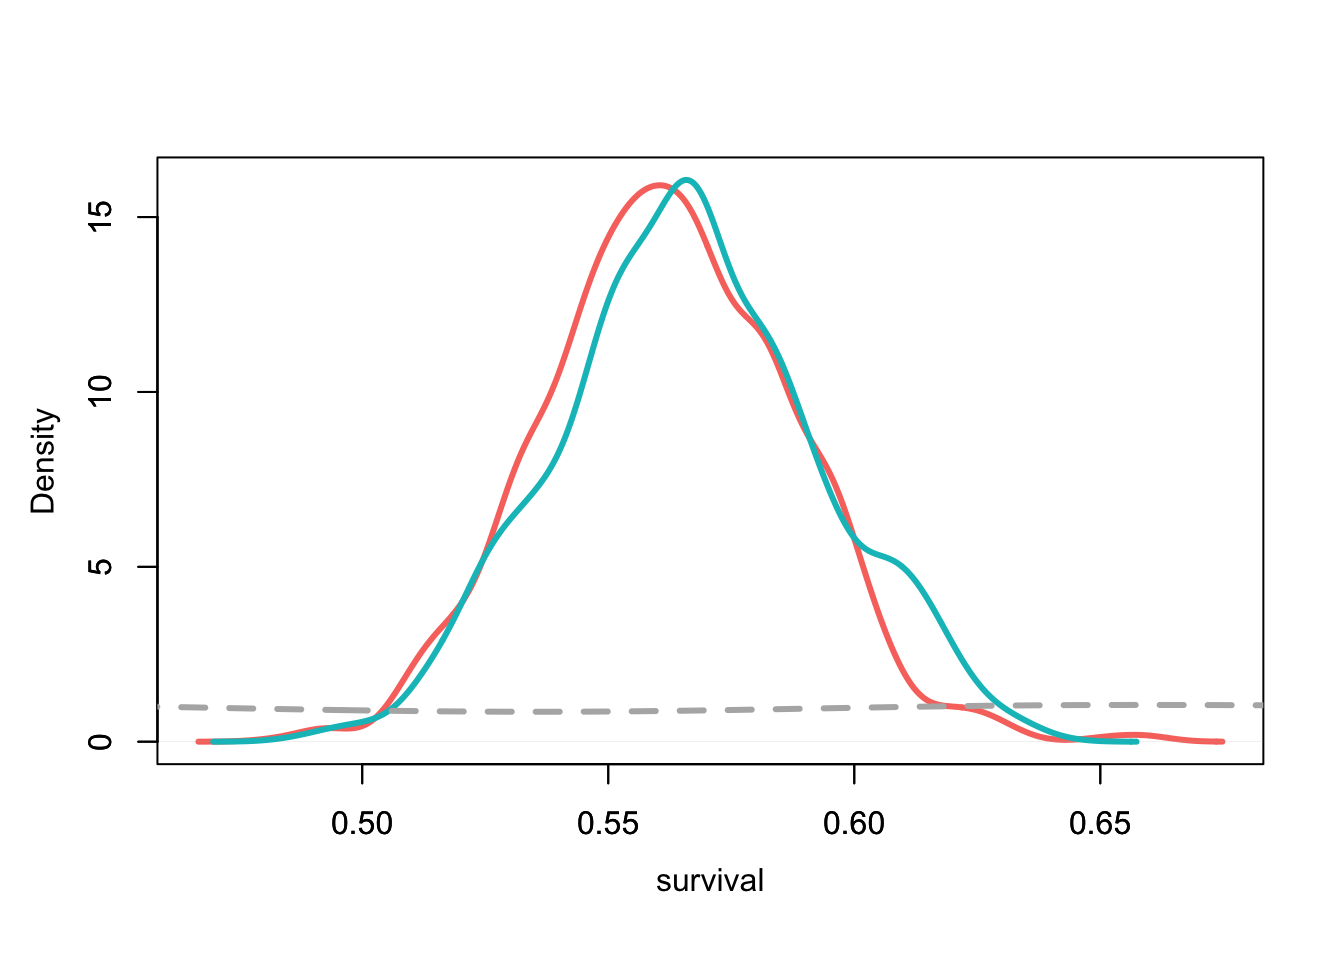
\includegraphics{banana-book_files/figure-latex/unnamed-chunk-194-1.pdf}

Posterior distribution of survival in color (two chains), prior in gray dashed line.

\hypertarget{how-to-incorporate-prior-information}{%
\section{How to incorporate prior information?}\label{how-to-incorporate-prior-information}}

Using information on body mass and annual survival of 27 European passerines, we can predict survival of European dippers using only body mass.

For dippers, body mass is 59.8g, therefore \(\phi = 0.57\) with \(\text{sd} = 0.073\).

Assuming an informative prior \(\phi_{prior} \sim \text{Normal}(0.57,0.073^2)\).

Mean posterior \(\phi_{posterior} = 0.56\) with credible interval \([0.52, 0.61]\).

No increase of precision in posterior inference.

\hypertarget{how-to-incorporate-prior-information-1}{%
\section{How to incorporate prior information?}\label{how-to-incorporate-prior-information-1}}

Now if you had only the three first years of data, what would have happened?

Width of credible interval is 0.53 (vague prior) vs.~0.24 (informative prior).

Huge increase of precision in posterior inference, a \(120\%\) gain!

\hypertarget{compare-survival-posterior-with-and-without-informative-prior}{%
\subsection{Compare survival posterior with and without informative prior}\label{compare-survival-posterior-with-and-without-informative-prior}}

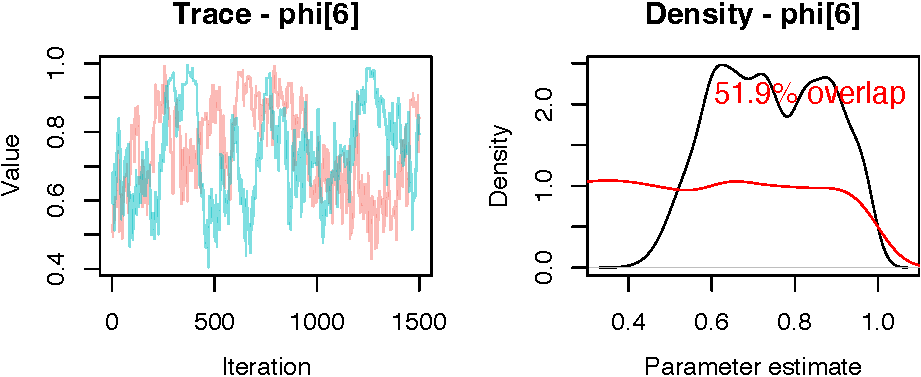
\includegraphics{banana-book_files/figure-latex/unnamed-chunk-195-1.pdf}

\hypertarget{prior-elicitation-via-moment-matching}{%
\section{Prior elicitation via moment matching}\label{prior-elicitation-via-moment-matching}}

The prior \(\phi_{prior} \sim \text{Normal}(0.57,0.073^2)\) is not entirely satisfying

Remember the Beta distribution

Recall that the Beta distribution is a continuous distribution with values between 0 and 1. Useful for modelling survival or detection probabilities.

If \(X \sim Beta(\alpha,\beta)\), then the first and second moments of \(X\) are:

\[\mu = \text{E}(X) = \frac{\alpha}{\alpha + \beta}\]

\[\sigma^2 = \text{Var}(X) = \frac{\alpha\beta}{(\alpha + \beta)^2 (\alpha + \beta + 1)}\]

\hypertarget{moment-matching}{%
\section{Moment matching}\label{moment-matching}}

In the capture-recapture example, we know a priori that the mean of the probability we're interested in is \(\mu = 0.57\) and its variance is \(\sigma^2 = 0.073^2\). Parameters \(\mu\) and \(\sigma^2\) are seen as the moments of a \(Beta(\alpha,\beta)\) distribution. Now we look for values of \(\alpha\) and \(\beta\) that match the observed moments of the Beta distribution \(\mu\) and \(\sigma^2\). We need another set of equations:

\[\alpha = \bigg(\frac{1-\mu}{\sigma^2}- \frac{1}{\mu} \bigg)\mu^2\]

\[\beta = \alpha \bigg(\frac{1}{\mu}-1\bigg)\]

For our model, that means:

\begin{Shaded}
\begin{Highlighting}[]
\NormalTok{(alpha }\OtherTok{\textless{}{-}}\NormalTok{ ( (}\DecValTok{1} \SpecialCharTok{{-}} \FloatTok{0.57}\NormalTok{)}\SpecialCharTok{/}\NormalTok{(}\FloatTok{0.073}\SpecialCharTok{*}\FloatTok{0.073}\NormalTok{) }\SpecialCharTok{{-}}\NormalTok{ (}\DecValTok{1}\SpecialCharTok{/}\FloatTok{0.57}\NormalTok{) )}\SpecialCharTok{*}\FloatTok{0.57}\SpecialCharTok{\^{}}\DecValTok{2}\NormalTok{)}
\DocumentationTok{\#\# [1] 25.65}
\NormalTok{(beta }\OtherTok{\textless{}{-}}\NormalTok{ alpha }\SpecialCharTok{*}\NormalTok{ ( (}\DecValTok{1}\SpecialCharTok{/}\FloatTok{0.57}\NormalTok{) }\SpecialCharTok{{-}} \DecValTok{1}\NormalTok{))}
\DocumentationTok{\#\# [1] 19.35}
\end{Highlighting}
\end{Shaded}

Now use \(\phi_{prior} \sim \text{Beta}(\alpha = 25.6,\beta = 19.3)\) instead of \(\phi_{prior} \sim \text{Normal}(0.57,0.073^2)\)

\hypertarget{prior-predictive-checks}{%
\section{Prior predictive checks}\label{prior-predictive-checks}}

\hypertarget{linear-regression}{%
\subsection{Linear regression}\label{linear-regression}}

Unreasonable prior \(\beta \sim N(0, 1000^2)\)

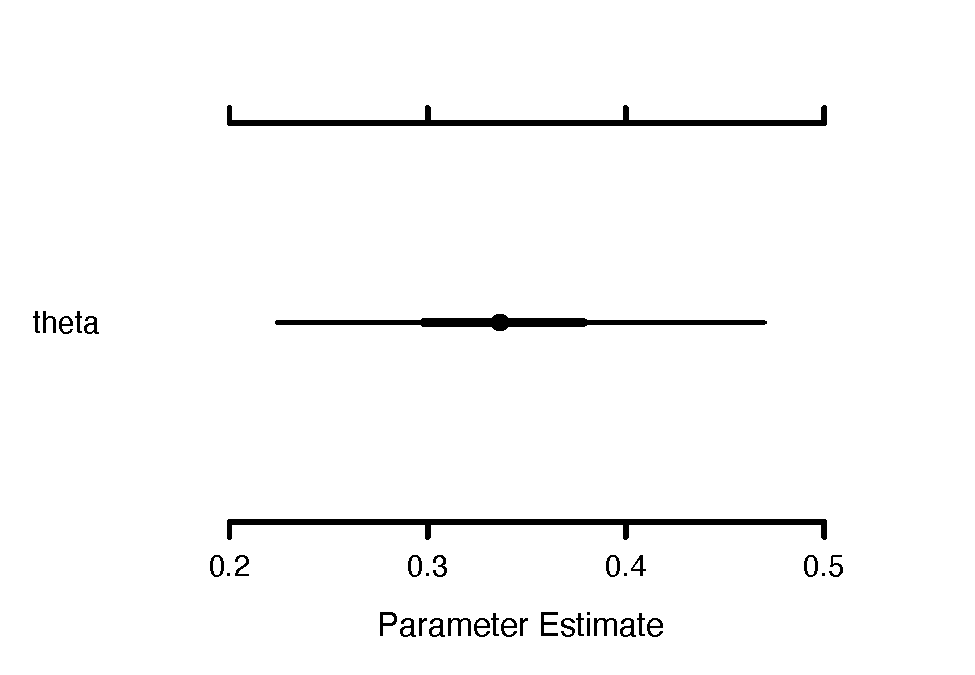
\includegraphics{banana-book_files/figure-latex/unnamed-chunk-197-1.pdf}

Reasonable prior \(\beta \sim N(2, 0.5^2)\)

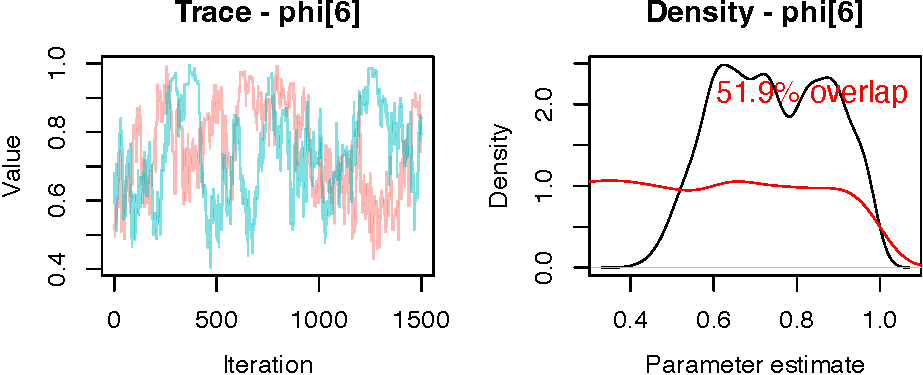
\includegraphics{banana-book_files/figure-latex/unnamed-chunk-198-1.pdf}

\hypertarget{logistic-regression}{%
\subsection{Logistic regression}\label{logistic-regression}}

Unreasonable prior \(\text{logit}(\phi) = \beta \sim N(0, 10^2)\)

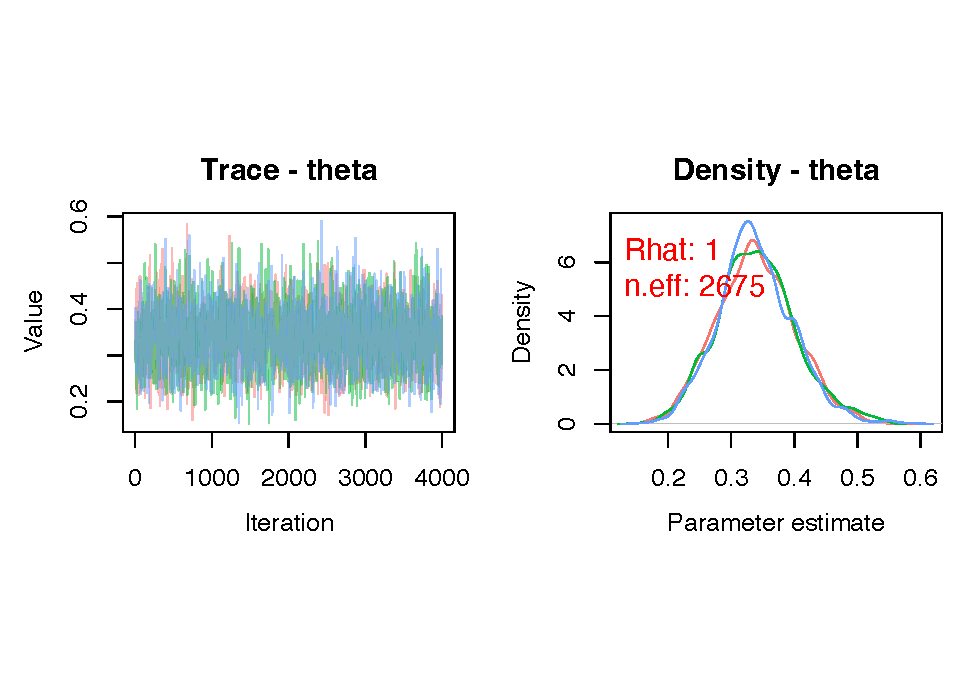
\includegraphics{banana-book_files/figure-latex/unnamed-chunk-199-1.pdf}

Reasonable prior \(\text{logit}(\phi) = \beta \sim N(0, 1.5^2)\)

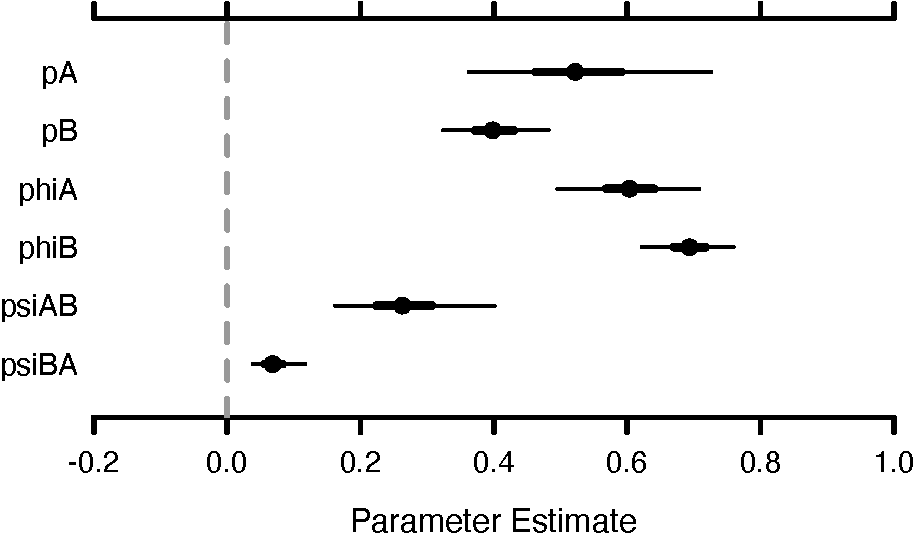
\includegraphics{banana-book_files/figure-latex/unnamed-chunk-200-1.pdf}

\hypertarget{capture-recapture-models-rely-on-assumptions}{%
\section{Capture-recapture models rely on assumptions}\label{capture-recapture-models-rely-on-assumptions}}

Design: No mark lost, Identity of individuals recorded without error (no false positives), Captured individuals are a random sample

Model: Homogeneity of survival and recapture probabilities, Independence between individuals (overdispersion)

Test validity of assumptions: These assumptions should be valid, whatever inferential framework, Use goodness-of-fit tests {---} Pradel et al.~(2005), \texttt{R} implementation with \href{https://besjournals.onlinelibrary.wiley.com/doi/full/10.1111/2041-210X.13014}{package \texttt{R2ucare}}, Posterior predictive checks can also be used (not covered; \href{https://arxiv.org/pdf/2011.01808.pdf}{Gelman et al.~2020}). Forward reference to chapter with gof and model selection.

\hypertarget{parameter-redundancy-issue}{%
\subsection{Parameter-redundancy issue}\label{parameter-redundancy-issue}}

\includegraphics{banana-book_files/figure-latex/unnamed-chunk-201-1.pdf}

Last survival and recapture probabilities cannot be estimated separately.

Poor mixing of the chains.

\begin{center}\rule{0.5\linewidth}{0.5pt}\end{center}

\hypertarget{parameter-redundancy}{%
\section{Parameter redundancy}\label{parameter-redundancy}}

Two issues

Intrinsic redundancy: Likelihood can be expressed by a smaller number of parameters; Feature of the model

Extrinsic redundancy: Model structure is fine, But lack of data makes a parameter non-estimable, Feature of the data.

\hypertarget{prior-posterior-overlap-for-phi_4-and-phi_6}{%
\section{\texorpdfstring{Prior-posterior overlap for \(\phi_4\) and \(\phi_6\)}{Prior-posterior overlap for \textbackslash phi\_4 and \textbackslash phi\_6}}\label{prior-posterior-overlap-for-phi_4-and-phi_6}}

\includegraphics{banana-book_files/figure-latex/unnamed-chunk-202-1.pdf}

\includegraphics{banana-book_files/figure-latex/unnamed-chunk-203-1.pdf}

\hypertarget{prior-posterior-overlap-for-p_3-and-p_7}{%
\section{\texorpdfstring{Prior-posterior overlap for \(p_3\) and \(p_7\)}{Prior-posterior overlap for p\_3 and p\_7}}\label{prior-posterior-overlap-for-p_3-and-p_7}}

\includegraphics{banana-book_files/figure-latex/unnamed-chunk-204-1.pdf}

\includegraphics{banana-book_files/figure-latex/unnamed-chunk-205-1.pdf}

\hypertarget{what-does-survival-actually-mean-in-capture-recapture}{%
\section{What does survival actually mean in capture-recapture ?}\label{what-does-survival-actually-mean-in-capture-recapture}}

Survival refers to the study area.

Mortality and permanent emigration are confounded.

Therefore we estimate apparent survival, not true survival.

Apparent survival probability = true survival × study area fidelity.

Consequently, apparent survival \textless{} true survival unless study area fidelity = 1.

Use caution with interpretation. If possible, combine with ring-recovery data, or go spatial to get closer to true survival.

\hypertarget{summary-3}{%
\section{Summary}\label{summary-3}}

\begin{itemize}
\item
  Blabla.
\item
  Blabla.
\end{itemize}

\hypertarget{suggested-reading-3}{%
\section{Suggested reading}\label{suggested-reading-3}}

\begin{itemize}
\item
  CJS state-space formulation \href{https://oliviergimenez.github.io/pubs/Gimenezetal2007EcologicalModelling.pdf}{Gimenez et al.~(2007)} and \href{https://onlinelibrary.wiley.com/doi/10.1111/j.1541-0420.2007.00891.x}{Royle (2008)}.
\item
  Work on missing values by \href{https://onlinelibrary.wiley.com/doi/abs/10.1111/j.1541-0420.2005.00399.x}{Bonner et al.~(2006)} and \href{https://projecteuclid.org/journals/annals-of-applied-statistics/volume-7/issue-3/Maximum-likelihood-estimation-of-markrecapturerecovery-models-in-the-presence-of/10.1214/13-AOAS644.full}{Langrock and King (2013)} and \href{https://link.springer.com/article/10.1007/s13253-014-0184-z}{Worthington et al.~(2015)}.
\item
  The example on how to incorporate prior information is in \href{https://besjournals.onlinelibrary.wiley.com/doi/abs/10.1111/j.1365-2664.2005.01101.x}{McCarthy and Masters (2005)}.
\item
  Combine live recapture w/ dead recoveries by \href{https://www.tandfonline.com/doi/pdf/10.1080/00063659909477230}{Lebreton et al.~(1999)} and go spatial to account for emigration \href{https://esajournals.onlinelibrary.wiley.com/doi/full/10.1890/12-0124.1}{Gilroy et al.~(2012)} and \href{https://besjournals.onlinelibrary.wiley.com/doi/full/10.1111/2041-210X.12134}{Schaub \& Royle (2014)}.
\item
  Non-identifiability in a Bayesian framework, see \href{https://oliviergimenez.github.io/pubs/Gimenezetal2009-weakidentifiability.pdf}{Gimenez et al.~(2009)} and \href{https://www.routledge.com/Parameter-Redundancy-and-Identifiability/Cole/p/book/9781498720878}{book by Cole (2020)}.
\end{itemize}

\hypertarget{part-iii.-states}{%
\part{III. States}\label{part-iii.-states}}

\hypertarget{introduction-6}{%
\chapter*{Introduction}\label{introduction-6}}


\hypertarget{part-iv.-case-studies}{%
\part{IV. Case studies}\label{part-iv.-case-studies}}

\hypertarget{introduction-7}{%
\chapter*{Introduction}\label{introduction-7}}


\hypertarget{part-v.-conclusion}{%
\part{V. Conclusion}\label{part-v.-conclusion}}

\hypertarget{take-home-messages}{%
\chapter*{Take-home messages}\label{take-home-messages}}


--\textgreater{}
--\textgreater{}

--\textgreater{}

--\textgreater{}

--\textgreater{}

\backmatter

  \bibliography{book.bib}

\printindex

\end{document}
